\documentclass[%
    12pt,
    english,
    onesided,
    a4paper,
    %BCOR=0mm,
    headsepline=true,
    numbers=noendperiod,
    appendixprefix=true  
]%
{book}
\usepackage{master}
%\addbibresource{references.bib}

\begin{document}

\pagestyle{plain}
\begin{titlingpage}



    \vspace*{5cm}
    \begin{center}
	Norwegian university of science and 		technology \\
	Faculty of information technology and 		electronical systems \\
	Department of mathematical sciences 
	\end{center}
	%\vspace{10pt}
    \rule[-11pt]{\textwidth}{1pt}
    \rule{\textwidth}{0.5pt}

    \begin{center}
    \Huge On formal DG-algebras 
    \end{center}

    \rule{\textwidth}{0.5pt}
    \rule[10.1pt]{\textwidth}{1pt}


    \begin{center}
    Torgeir Aambø
    \end{center}



    \vspace{\fill}



\end{titlingpage}\clearpage

\frontmatter


\section{Abstract}

A differential graded algebra (DG-algebra) can often be thought of as an algebraic gadget containing highly detailed information about a topological space. Two such cases are the algebra of cochains, and the cohomology ring. The latter is often easy to calculate, but the former contains in general much more information about the space we are interested in. In this thesis we explore the relationship between these two DG-algebras---more precisely some situations where these two algebras contain the same homotopical information. Such algebras are called formal DG-algebras.

In order to understand which type of homotopical information a DG-algebra can contain, we construct obstructions to formality through higher cohomology operations. We then generalize DG-algebras to $\A$-algebras, and look at some ways to use this generalized theory as a unified framework for both DG-algebras, and higher order cohomology operations. This framework allows us to prove that a certain class of topological spaces---namely those with Lusternik-Schnirellmann category $1$---have formal cochain algebras. \clearpage


\section{Sammendrag}

En \textit{differensialgradert algebra} (DG-algebra) kan ofte sees på som en samling av høyt detaljert topologisk informasjon. To slike tilfeller er algebraen av kokjeder, og kohomologiringen til et topologisk rom. Den sistnevnte er ofte lett å regne ut, men den førstnevnte innholder generelt mye mer informasjon om rommet vi er interessert i. I denne avhandlingen utforsker vi forholdet mellom disse to algebraene---mer presist noen situasjoner hvor disse to innholder den samme homotopiske informasjonen. Slike algebraer kalles \textit{formelle} DG-algebraer. 

For å forstå hvilken type homotopisk informasjon en DG-algebra kan inneholde, konstruerer vi hindringer for formalitet gjennom høyere ordens kohomologioperasjoner---kalt \textit{Massey produkter}. Vi generaliserer så DG-algebraer til \textit{$\A$-algebraer}, og ser på noen måter å bruke denne generaliserte teorien som et felles rammeverk for både DG-algebraer og Massey produkter. Dette rammeverket tillater oss å vise at en viss klasse av topologiske rom---nemlig de med Lusternik-Schnirelmann kategori 1---har formelle kokjede algebraer. \clearpage


\section{Acknowledgments}

This thesis is the conclusion to my five year long mathematical endeavor at NTNU, and the five best years of my life so far. 

These years would not have quite different, had it not been for my supervisor, Gereon Quick. I owe him a lot for showing me the joy and depths of topology, for years of learning, inspiration and motivation, and for guiding me through this thesis. 

These years would also have been quite different, had it not been for the mathematical community at NTNU, especially ``Matteland'', which has been my second home for many years. It has been a platform for motivation, highly interesting conversations and fruitful discussions about mathematics and its set theoretic complement. 

I also want to thank all my friends in Delta---the student association for mathematics and physics---for allowing me to do other things outside of mathematics, and for encouraging me to grow as a person. The real masters degree is of course the friends we made along the way. 

Finally, I want to thank my family and my girlfriend, for their relentless love and support for all that I do, and have done over the years. 

\hspace{\fill} - Torgeir Aambø\clearpage


\section{For experienced readers}

This thesis is not meant to be short and concise---as this is in our opinion not the best way to deeply understand abstract mathematics, which after all is our main goal. For this reason there will be some lengthy explanations and some lengthy calculations in order to properly understand the material at hand. There will also be some intentionally vague sentences in order to build intuition and a more natural feeling for the theory. 

The two first sections in chapter 3---on transferring algebraic structures through homotopy equivalences---are not much needed for the thesis, but they give good motivation for why the definition on an $\A$-algebra is the way it is. The two subsections of chapter 3 on using rooted trees as a visual understanding of the relations in DG-algebras, $\A$-algebras and their morphisms, are also not needed to understand the later results, but they too serve as intuition for the relations, and how to use them. These can easily be omitted by readers who have already seen these concepts. 

If a reader wants to more quickly understand the meat of the thesis---or only go through the most important result---I have added below a list of where to find the central definitions and results. There is also a summary at the end, which quickly summarizes what has been done throughout the thesis. 

\begin{enumerate}
	\item Definition 1.4. (DG-algebra)
	\item Example 1.8. (Cohomology algebra)
	\item Definition 1.15. (Quasi-isomorphic DG-algebras)
	\item Definition 1.16. (Formal DG-algebra)
	\item Definition 2.4. (Massey products)
	\item Definition 2.5. (Vanishing Massey products)
	\item Theorem 2.10. (Formal $\implies$ vanishing Massey products)
	\item Definition 3.3. ($\A$-algebra)
	\item Definition 3.6. ($\A$-quasi-isomorphism)
	\item Theorem 3.10. (Kadeishvili's theorem)
	\item Corollary 3.15. (Trivial $\A$-structure $\implies$ formal)
	\item Theorem 3.23. (Vanishing Massey products + + $\implies$ formal)
	\item Corollary 4.10. ($\ls(X)\leq 1$ $\implies$ $X$ formal)
\end{enumerate}

We will try to explain all the details as they come up, but we do not at all claim that this thesis is self contained. We assume some familiarity with homological algebra and algebraic topology, as well as some general mathematical maturity. 

All images and diagrams are made by the author. \clearpage
\vspace*{-1cm}
\tableofcontents\clearpage

\section{Introduction}

The field of algebraic topology is centered around using objects, techniques and theory from abstract algebra---in order to study topological spaces. As both algebra and topology are vast and deep fields, there are countless ways of using both theories in tandem to produce interesting results and deep connections between the two fields. A highly successful algebraic construction---now used throughout the whole field of mathematics, but originally arising from trying to study topological spaces---is called cohomology. 

Cohomology is a graded algebra---associated to any topological space---where the elements are essentially those closed subspaces that are not the boundaries of other subspaces. This allows us to study how many, and which kinds of holes a topological space has---which is one of its central topological properties. There are many ways of calculating the cohomology of a space, but by definition they arise as quotients of collections of cochains in the topological space---which can by thought of as the closed subspaces. The collection of all cochains form what we call the cochain algebra of the topological space, and it gives a very rich insight into the space we are interested in. An unfortunate drawback is that this cochain algebra is very difficult to calculate, much harder that the cohomology, hence we most often this instead. 

As the cohomology is easier to understand---and easier to calculate---we arrive at the following question: If two topological spaces have the same cohomology algebra, do they also have the same cochain algebra? The answer to this turns out to be no. In general, there are certain bits of information---for example \emph{Massey products}---stored in the cochain algebra, that the cohomology algebra does not have access to. This means that two different topological spaces, with different cochain algebras, could have the same cohomology algebra, but by using the existence of these Massey products---which are certain higher order, higher arity, cohomology operations---allows us to distinguish them. 

As a follow up to the failure of the previous question, we can ask: Given the cochain algebra of a topological space, how can I know whether it is sufficiently simple, such that the cohomology algebra has access to all the relevant information? Such ``sufficiently simple'' algebras are called \emph{formal} algebras, and they are the central theme of this thesis. More precisely, an algebra is called formal if it contains the same homotopical information as its cohomology algebra, which means we must find some way to relate these two. This is done through quasi-isomorphisms. 

The above informal question turns out to be very deep and interesting, so we take it as the central question we want to answer in the whole thesis. 

\begin{central}
Given the cochain algebra $C(X)$ of a topological space $X$, how do we know whether $C(X)$ is sufficiently simple, such that $H(X)$---the cohomology algebra of $X$---has access to all the relevant information?
\end{central}

This is of course an imprecise and non-mathematical question, as ``sufficiently simple'', ``access'' and ``information'' are not yet well defined mathematical concepts. Thus we will need to define these parts, and refine the question more mathematically throughout the thesis. In order to tell a cohesive story, and to have something to look ahead for, we give the precise question:

\begin{central}
Given a DG-algebra $A$, how can we know if it is formal?
\end{central}

We see that we have a lot of work ahead of ourselves, so lets define the goals we want to achieve. 

Our \textit{first goal} for this thesis is simply to learn about mathematics that we previously did not know much about, as well as answering the above central question. This is done through two attempts. The first one is using Massey products, which although they give obstructions to formality, turn out to not be the only possible obstructions. We then try to generalize DG-algbras and Massey products to a unified and stronger framework, called $\A$-algebras, which we successfully use to get one possible solution to the central question. 

The \textit{second goal} is to push the boundaries of mathematical knowledge, by whatever tiny nudge we can. After developing the above-mentioned theory, we are able to provide a new case where formality is guaranteed. This somewhat rectifies the failure of Massey products to be the only obstructions to formality, by proving that they are in fact the only obstructions in DG-algebras where the induced product on cohomology is trivial. We then apply this new result to an example from topology, in order to prove a known result---that spaces with Lusternik-Schnirelmann category 1 are formal---in a new way. 

The \textit{third goal} is to make a rigorous, thorough, detailed---but still understandable---presentation of formal DG-algebras, their connection to Massey products and in the end---their partial common framework in $\A$-algebras. This is so that others---also wanting to understand the material---can look at a cohesive story, and not have to dig up all the relevant results and literature themselves. 
 
 






\clearpage


\section{Overview of the thesis}

\textit{\Cref{ch:1}} is spent on defining DG-algebras, seeing some examples and  defining formality for DG-algebras. The latter half of it is designated to introducing the general theory which allows us to have a homotopy theory for DG-algebras, called model categories---as well as proving that DG-algebras admit such a theory. Together these two parts should answer what we meant by ``sufficiently simple'' and ``has access to'' in the introduction.

\textit{\Cref{ch:2}} is an interlude into the ``information'' part of the central question. We introduce certain algebraic operations---called Massey products---that serves as ``information'' in the DG-algebra. We then prove that this information is not accessible to the cohomology algebra, and that all Massey products must vanish if the DG-algebra is formal. 

\textit{\Cref{ch:3}} is another interlude, this time into transferring algebraic structures between objects. This chapter is not an integral part of the thesis, but  it is meant to give strong intuition into how the algebraic objects we introduce in \ref{ch:4} behave. In this chapter we try to deform a DG-algebra by a deformation retraction, to see if the result is still a DG-algebra. 

\textit{\Cref{ch:4}} introduces a new algebraic object called $\A$-algebras. These objects generalize the DG-algebras we develop in \cref{ch:1}. This added generalization gives a better behaved homotopy theory, as well as making the central question nice and easy to state and answer. In the second part of the third chapter we prove a new---as far as the author is aware---result, introducing a special case where if the Massey products we developed in \cref{ch:2} all vanish, we must have a formal DG-algebra. 

\textit{\Cref{ch:5}} is then spent trying to find an interesting example to the new result we proved at the end of \cref{ch:3}. We show that a certain class of topological spaces---those with Lusternik-Schnirelmann category 1---satisfy the requirements of the theorem, and hence that they must be formal spaces. 

Lastly, we have two appendices. 

\textit{\Cref{ap:A}} features two long proofs that were omitted during the thesis in order to not break the flow of reading. The first proves that the deformed DG-algebra from \Cref{ch:3} is not associative, but associative up to homotopy. The second proves that a certain decomposition of a DG-algebra gives us a deformation retraction onto its cohomology algebra.

\textit{\Cref{ap:B}} is added to showcase an alternative method to constructing the model structure on the category of DG-algebras. This alternative construction uses monoids in monoidal model categories. 


\clearpage



\mainmatter
\pagestyle{fancy}
\newpage
\chapter{DG-algebras}
\label{ch:1}
\tikz[remember picture,overlay]\node[opacity=1,inner sep=0pt] at (current page.center)%
{
\includegraphics[%
clip,
width=1.05\paperwidth,
height=1.05\paperheight
]{chaptertitles/ch1.pdf}};

\clearpage





\section{Motivation}

The theory of homology was a theory long in development. Luckily for us we have access to good historical records---like \cite{history1} and \cite{history2}---which this overview is based on. 

Homology theory arguably started with Riemann in \cite{riemann}, where he defined ``connectedness numbers''. Some years later these were generalized to higher dimensions by Betti in \cite{betti}, which became the numbers we today call Betti numbers. There were some problems and mistakes in both the above papers, so a more rigorously defined and developed notion of these were given by Poincaré in the famous paper ``Analysis situs'' (\cite{situs}). 

Due to some mistakes and new developments, Poincaré published a complement to ``Analysis situs'' (\cite{situs2}), where in addition the first use of a prototype of the singular chain complex of a polyhedron was used. 

The theory of these chains on topological spaces, and their Betti numbers were more firmly joined together, when Noether claimed in an abstract for a lecture series (\cite{noether}) that these in fact form abelian groups - being the first case of the homology groups we use today. 

Inspired by these ideas, Mayer constructed in \cite{mayer, mayer2} the modern notion of a chain complex, and its homology, beginning the journey of a purely algebraic description of topological information. Some years later the theory of cohomology, and cup products was developed by both Alexander and Kolmogoroff. They both had some mistakes and ad hoc definitions, so a more refined and developed theory was given by Whitney in \cite{whitney}. In this paper, Whitney also introduced ``the Leibniz axiom''. This implicitly defined the notion of what we call a differential graded algebra (DG-algebra) in modern terminology, namely as a cohomology ring satisfying this Leibniz axiom. This object is the focus of most of this thesis.

We start the chapter by developing these DG-algebras for ourselves, as well as look at very special kind of DG-algebra---referred in the introduction to as ``sufficiently simple''. Afterwards we develop the abstract concept of homotopy theory. We do this in order to prove that DG-algebras admit such a homotopy theory, which might not be a surprising fact given their above described connection to topology. The main result from this chapter is a description of formality, using only a single span of quasi-isomorphisms, i.e. 

\textbf{Theorem A. } \textit{A DG-algebra $A$ is formal, if and only if there is	a span of quasi-isomorphisms $H(A)\leftarrow B	\rightarrow A$, for some DG-algebra $B$.}


\section{The algebraic model}

Our algebraic model consists of DG-algebras, which are both algebras, and cochain complexes in a compatible way. We define them by first looking at their different structures. For the rest of this thesis, we let $k$ be an infinite field, unless otherwise stated.  

\begin{definition}[Algebra]
An algebra over $k$, also called a $k$-algebra, is a vector space $A$ over $k$, together with a bilinear map $m: A\times A\rightarrow A$, usually called multiplication. More precisely, $m$ is a map satisfying 
\begin{itemize}
    \item $m(x+y, z) = m(x, z) + m(y, z)$
    \item $m(x, y+z) = m(x, y) + m(x, z)$
    \item $m(ax, by) = (ab)m(x, y)$
    \item $m(m(x, y), z) = m(x, m(y, z))$
\end{itemize}
for all $x, y , z \in A, a, b\in k$. 
\end{definition}

Notice in particular that we don't require our map $m$ to be commutative. The last condition says that the product is associative, but we remark that not all authors require this in general. By convenience, we often replace $m(x, y)$ by just $x\cdot y$ or simply $xy$. We will switch a bit between all these three where they make the most sense to use. 

It can be noted that we can define algebras over rings in general---not just fields--- but we chose this definition as it will be sufficient for us throughout the thesis. It will also generalize more smoothly to $\A$-algebras in chapter 3. 

\begin{definition}[Graded algebra]
We say an algebra $A$ is a graded algebra if there is a decomposition $A = \bigoplus_{n\in \Z}A^n$, into vector spaces $A^n$, such that the product respects the grading, i.e. $m:A^n\times A^m \rightarrow A^{n+m}$. 
\end{definition}

To be able to tie these graded algebras in with the already well developed theory of homological algebra and algebraic topology, we need to have some way to build cohomology. This is done through the notion of cochain complexes. 

\begin{definition}[Cochain complex]
A cochain complex $(A^{\bullet}, d^{\bullet})$ is a sequence of Abelian groups, or modules,
\begin{equation*}
    \ldots, A^{n-1}, A^n, A^{n+1}, A^{n+2}\ldots
\end{equation*}
together with maps $d^n:A^n\rightarrow A^{n+1}$ such that $d^{n+1}\circ d^n = 0$ for all $n$. Such a structure is usually visualized as a sequence of the following form
\begin{equation*}
    \cdots\longrightarrow A^{n-1} \overset{d^{n-1}}\longrightarrow A^n \overset{d^n}\longrightarrow A^{n+1} \overset{d^{n+1}}\longrightarrow A^{n+2}\longrightarrow\cdots
\end{equation*}
\end{definition}

The following definition is one of the main definitions of the thesis, so make sure to digest it properly. It is a combination of the (graded) algebra structure and the cochain complex structure, into one unified framework. 

\begin{definition}[Differential graded algebra]
A differential graded algebra $(A, d)$, often called just a DG algebra or a DGA, is a graded algebra $A$ together with a degree $+1$ map $d: A\rightarrow A$, often called the differential, such that 
\begin{itemize}
    \item $d\circ d = 0$, and
    \item $d(a\cdot b) = d(a)\cdot b + (-1)^{|a|}a\cdot d(b)$. 
\end{itemize}
\end{definition}

The condition that $d\circ d = 0$ is what makes $A$ into a cochain complex, and the second condition is what makes these two structures work well together. The second condition is called the graded Leibniz rule, or the Leibniz axiom. The criteria that $d$ has degree $+1$ means that if we take a homogeneous element $a$ of degree $n$, i.e. an element in $A^n$, then $d(a)$ has degree $n+1$, i.e. it lies in $A^{n+1}$. We will use the following notation if the degree of an element $a$ is $n$, $|a|=n$. Similarly for morphisms, for example $|d|=-2$. By some abuse of notation, we will denote a DG-algebra simply by $A$.

% \begin{definition}{Chain maps}
%     A morphism of cochain complexes $f:(A^{\bullet}, d^{\bullet})\rightarrow (B^{\bullet}, b^{\bullet})$ is a family of maps $f^n:A^n\rightarrow B^n$, such that $f^{n+1}\circ d^{n} = b^n\circ f^{n}$, in other words, each square in the following diagram commutes
%     \begin{center}
%     \begin{tikzcd}
%         \cdots \arrow[r] & A^{n-1} \arrow[r, "d^{n-1}"] \arrow[d, "f^{n-1}"] & A^{n} \arrow[r, "d^{n}"] \arrow[d, "f^{n}"] & A^{n+1} \arrow[d, "f^{n+1}"] \arrow[r, "d^{n+1}"] & A^{n+2} \arrow[d, "f^{n+2}"] \arrow[r] & \cdots \\
%         \cdots \arrow[r] & B^{n-1} \arrow[r, "b^{n-1}"]                      & B^{n} \arrow[r, "b^{n}"]                    & B^{n+1} \arrow[r, "b^{n+1}"]                      & B^{n+2} \arrow[r]                      & \cdots
%     \end{tikzcd}
%     \end{center}
% \end{definition}


As these objects will be one of our main focus points throughout this thesis, it is important to have control over some examples. In the introduction we used the word ``cochain algebra'' to mean roughly any DG-algebra that we can associate to a topological space. So to tie the theory to the introduction we focus mostly on the examples coming from topology. Most of these are related to cohomology in some way. This is maybe not surprising given the historical context earlier. 

\begin{example}[Singular $mod\,p$ cohomology]
Let $T$ be a topological space. For any prime number $p\neq 2$, the singular $mod p$ cohomology ring $H^*(T, \Z/p\Z)$, is a DG algebra. Its graded multiplication is the induced operation in cohomology from the cup product of n-cochains. The differential is a bit more involved, but comes from the exact sequence
\begin{equation*}
\Z/p\Z \rightarrow \Z/p^2 \rightarrow \Z/p\Z.
\end{equation*}    
This induces a long exact sequence 
\begin{equation*}
    \cdots \rightarrow H^i(T; \Z/p\Z) \rightarrow H^i(T; \Z/p^2\Z) \rightarrow H^i(T; \Z/p\Z) \overset{\beta}\rightarrow H^{i+1}(T; \Z/p\Z) \rightarrow \cdots, 
\end{equation*}
where the connecting homomorphism $\beta$ is called the Bockstein homomorphism. This homomorphism serves as the differential in our DG-algebra $H^*(T, \Z/p\Z)$. 
\end{example}

\begin{example}[The singular cochain algebra]
Let $X$ be a topological space and $k$ a field. An $n$-cochain on $X$ is a group homomorphism $S_n(X)\longrightarrow k$, where $S_n(X)$ is the group of singular $n$-chains, i.e. the free group on the set of continuous map $\sigma\colon\Delta^n\longrightarrow X$, where $\Delta^n$ is the standard $n$-simplex. 

The group of singular $n$-cochains on $X$ is then defined to be 
\begin{equation*}
S^n(X;k) = Hom_{Ab}(S_n(X), k)
\end{equation*}
We define the coboundary operator to be the group homomorphism
\begin{align*}
	\delta\colon S^n(X;M)&\longrightarrow S^{n+1}(X;M) \\
	c &\longmapsto [\sigma\mapsto c(\partial_{n+1}(\sigma))]
\end{align*}
where $\partial_{n+1}$ is the boundary operator on the groups of singular $n$-chains. This operator makes the set $\{S^i(X;M)\}$ into a cochain complex. 

The multiplication is the so-called cup product of cochains. For a good rigorous treatment of this operation, see \cite[Section 3.2.]{hatcher}. 
\end{example}

\begin{example}[The cohomology algebra of a DG-algebra]
Since every DG algebra is a cochaincomplex, it naturally comes equipped with a way to form its cohomology, by simply letting $H(A)=Ker(d)/Im(d)$. The cohomology of any cochain complex is naturally graded, and together with the induced product from the DG algebra, it forms a graded algebra. 
    
The product on the cohomology algebra is defined by $[a][b]=[ab]$, and it is well defined because any other two representatives $a'=a+d(t)$ and $b'=b+d(r)$ has a product $[a'b']=[ab+ad(r)+d(t)b+d(t)d(r)]$. The last three are coboundaries because $d(ar)=d(a)r + (-1)^{|a|}ad(r) = (-1)^{|a|}ad(r)$ since $a$ is a cocycle. Hence $ad(r)$ is the boundary of $(-1)^{|a|}(ar)$. Similarily $d(tb)$ is the boudary of $tb$ and $d(t)d(r)$ is the boundary of $td(r)$. Hence all representatives give the same class in cohomology, and the product is well defined. 
    
We can also trivially equip the cohomology algebra with the differential $d_H=0$, which turns the cohomology algebra into a DG-algebra. 
\label{ex:cohomology}
\end{example}

Note that the cohomology algebra of the singular cochain algebra of a topological space $X$, is the singular cohomology ring of $X$.

\begin{example}[Tensor algebra]
Let $V$ be a vector space over a field $k$ with basis $e_1, \cdots, e_n$. Define a graded vector space $T(V)$ by letting its graded components be give by
\begin{equation*}
    T^k(V) = \bigoplus_{i=1}^k V^{\otimes i}.
\end{equation*}
We define the differential $d\colon T^k(V)\longrightarrow T^{k-1}(V)$ component-wise by
\begin{equation*}
    d(e_{i_1}\otimes \cdots \otimes e_{i_k}) = \sum_{i_1\leq i_j\leq i_k}(-1)^{i_j}e_{i_1}\otimes \cdots \otimes \widehat{e_{i_j}}\otimes \cdots \otimes e_{i_k}
\end{equation*}
where $\widehat{i_j}$ means that the $j$'th component is omitted. The product is given by tensor concatenation, i.e. 
\begin{equation*}
    (e_{i_1}\otimes \cdots \otimes e_{i_k})\cdot(e_{j_1}\otimes \cdots \otimes e_{j_r}) = e_{i_1}\otimes \cdots \otimes e_{i_k}\otimes e_{j_1}\otimes \cdots \otimes e_{j_r}
\end{equation*}
\end{example}

Notice that this example actually uses the opposite grading of what we used in the definition. This is called having homological grading, instead of our cohomological grading. We won't use this example for anything in the thesis, so the different grading does not matter, but, it is an important example for much of related theory, for example the deformation theory of algebras. 

\subsection*{Interlude on rational homotopy theory}

The next example requires a bit to set up. It is called the piece-wise linear de Rham algebra, and comes from the field of rational homotopy theory. Because this theory is central for the development of DG-algebras, and formality, we give a bit of background information. 

A famous---notoriously difficult---problem in algebraic topology, is to calculate the homotopy groups of the spheres. The $n$'th homotopy group of a space $X$ is essentially the set of continuous maps from $S^n$---the $n$-dimensional sphere---to $X$, where we identify two such maps if they are in some sense topologically similar. It turns out that higher dimensional spheres can twist around lower dimensional spheres non-trivially---producing many non-trivial homotopy groups. Even worse is maybe the fact that they seem to satisfy no general pattern at all. 

As a way to get around this, Serre looked at what happens if one works over the rationals instead of the integers, essentially removing the difficult torsion from the theory. In \cite{Serre} he successfully calculated the torsion free part of all homotopy groups of all spheres, starting a journey for mathematicians to develop a complete torsion free theory of topological spaces. This theory is now called rational homotopy theory, and its development was mainly spearheaded by Quillen and Sullivan. One of the great achievements in this field came from developing purely algebraic models for the theory, meaning that one could only study some algebraic objects, and get all information about the topological spaces. More formally, we get that the rational homotopy type of a topological space is given by the isomorphism class of its algebraic model. The first successful attempt at making such an algebraic model was made in \cite{Quillen} in 1969 by Quillen, using certain differential graded Lie algebras (DGL-algebras). Some years later Sullivan---inspired by the de Rham theory for manifolds---proposed in \cite{Sullivan} a simpler idea for a purely algebraic model for rational homotopy theory, using certain DG-algebras. 

In the following definition we use so-called simplicial DG-algebras. These are functors $\Delta \longrightarrow DGA_k$, where $\Delta$ is the simplex category. We haven't really discussed morphisms of DG-algebras yet---hence not defined the category $DGA_k$---but the reader can use their imagination to convince themselves that such a category should exist. The morphisms will be covered in the next section, so it is also possible to peek at the definition, and then come back to this example afterwards. 

\begin{definition}
Let $\mathcal{A}_*$ be the DG-algebra given by 
\begin{equation*}
    \mathcal{A}^n_* = k(t_0, \ldots, t_n, dt_0, \ldots, dt_n)/(1-\sum_{i=0}^n t_i, \sum_{i=0}^n dt_i) 
\end{equation*}
where $|t_i|=0$. This is in fact a simplicial DG-algebra, where the face and degeneracy maps are respectively given by 
\begin{align*}
    \partial_i\colon \mathcal{A}_*^n &\longrightarrow\mathcal{A}_*^{n-1} \\
    t_j&\longmapsto
    \begin{cases}
        t_j, \quad j<i \\
        0, \quad j=i \\
        t_{j-1}, \quad j>i
    \end{cases}
\end{align*}
and 
\begin{align*}
    s_i\colon \mathcal{A}_*^n &\longrightarrow\mathcal{A}_*^{n+1} \\
    t_j&\longmapsto
    \begin{cases}
        t_j, \quad j<i \\
        t_j+t_{j+1}, \quad j=i \\
        t_{j+1}, \quad j>i
    \end{cases}
\end{align*}
\end{definition}

\begin{definition}
Let $S$ be a simplicial set. We define a functor $\mathcal{A}\colon sSet\longrightarrow DGA_\Q$ by sending $S$ to $Hom_{sSet}(S, \mathcal{A}_*^*)$. The DG-algebra structure is defined object-wise.
\end{definition}


\begin{example}[Piece-wise linear de Rham algebra]
We define the DG-algebra of piece-wise linear de Rham forms on a topological space $X$ to be the DG-algebra given by
\begin{equation*}
    \Apl(X) = \mathcal{A}(Sing(X))
\end{equation*}
where $Sing(X)$ is the set of continuous maps from $\Delta^n$---the standard $n$-simplex---to $X$. 
\end{example}

Notice here that $\Apl(X)$ is actually a commutative DG-algebra, often denoted CDG-algebra. The DG-algebra of rational cochains on a topological space is not commutative in general, which is one of the reasons this $\Apl$ construction is introduced. However, the rational singular cohomology algebra of a topological space \emph{is} commutative, so $\Apl(X)$ being commutative allows rational homotopy theory to be simplified, as the category $CDGA_\Q$ of commutative rational DG-algebras is a bit nicer to work with than $DGA_\Q$. This added niceness is not needed in our case as we are interested in a property that does not depend on commutativity.  




\section{Formality}
\label{sec:formality}

Hopefully the reader was able to imagine some definition of morphism between DG-algebras in order to get the earlier example---using the category $DGA_k$---to work. If not then we include the definition now. 

\begin{definition}[DG morphism]
Let $(A, d_A)$ and $(B, d_B)$ be two DG-algebras. A map $f:A\longrightarrow B$ is called a morphism of DG-algebras---sometimes shortened DG-morphism---if it
\begin{itemize}
    \item preserves the degree of homogeneous elements, i.e. if $a\in A^n$ then $f(a)\in B^n$, and
    \item commutes with the differentials, i.e. $f(d_A(a))=d_B(f(a))$. 
\end{itemize}
\end{definition}

This implies that we can think of a morphism of DG-algebras as a regular morphism of algebras in each degree, which respects the differential.

The collection of DG-algebras over some field $k$, together with these morphisms form a category, which we already know we will denote by $DGA_k$. There are some special types of morphisms in $DGA_k$ that will be important throughout the thesis. As usual we say a morphism is an isomorphism if it has a two-sided inverse. Given this, the following definition is especially important. 

\begin{definition}[Quasi-isomorphism]
Let $(A, d_A)$ and $(B, d_B)$ be two DG-algebras. A morphism $q:A\longrightarrow B$ is called a quasi-isomorphism if the induced map $\Bar{q}:H(A)\rightarrow H(B)$ on their cohomology algebras, is an isomorphism. We often write $q:A\overset{\sim}\longrightarrow B$ if $q$ is a quasi-isomorphism. 
\end{definition}

\begin{definition}[Quasi-isomorphic DG-algebras]
We say two DG-algebras $(A, d_A)$ and $(B, d_B)$ are quasi-isomorphic if they can be connected by a zig-zag of quasi-isomorphisms 
\begin{equation*}
    A \overset{\sim}\longleftarrow \bullet \overset{\sim}\longrightarrow \cdots \overset{\sim}\longleftarrow \bullet \overset{\sim}\longrightarrow B .
\end{equation*}
This is sometimes also referred to as $A$ and $B$ being weakly equivalent. The reason for this alternative name will become clear when we discuss model categories in the next section. 
\end{definition}

With this we finally can state the definition of the informal description ``sufficiently simple'' that we used in the introduction. This definition is the central definition of the thesis, and is the property we will be focusing on for the rest of it. 

\begin{definition}[Formal DG-algebra]
A DG algebra $(A, d)$ is called formal if it is quasi-isomorphic to a DG algebra $(M, 0)$ with trivial differential. 
\end{definition}

This definition is often stated as $A$ being quasi-isomorphic to its cohomology algebra, treated as a DG algebra in the way described in \ref{ex:cohomology}. This is equivalent, because if $A$ is formal then the zig-zag of quasi-isomorphisms $M \leftarrow \cdots \rightarrow A$ induces isomorphisms $H(M)\cong \cdots \cong H(A)$, but as $M$ had a trivial differential---its cohomology is equal to itself. Hence we have $M\cong H(A)$, and we can extend the zig-zag of quasi-isomorphisms to $H(A)\cong M \leftarrow \cdots \rightarrow A$, which is also a zig-zag of quasi-isomorphisms. This means that $A$ is quasi-isomorphic to its cohomology algebra $H(A)$. 

So what does it mean for a DG-algebra to be formal? And is there a justification for its name? Formality for DG-algebras was first defined in \cite{DGMS} and was used as a tool to describe the real homotopy theory of certain manifolds. In the paper the authors define a certain DG-algebra for these manifolds---called their minimal models---and define the manifold to be formal if its minimal model is formal as a DG-algebra. The notion of being formal then means that we can ``formally reconstruct'' the minimal model from its cohomology algebra. The former is often very hard to describe in full detail as it is very rich in information, while the latter is often simple to calculate for many manifolds. Thus, formality means that our DG-algebra is simple enough, and does not contain ``too much information'', meaning that having calculated the cohomology algebra automatically ``gives us'' the minimal model---at least up to quasi-isomorphism. This is of course not precise at all, but in our opinion it serves as some good intuition. When this is the case we say that the real homotopy type of the manifold is a formal consequence of its cohomology. 

So, the intuitive slogan for the definition of formality for manifolds, and more generally for any DG-algebra, is a DG-algebra where all its homotopy-information is contained in its cohomology algebra.

We can finally restate the central question of the thesis with an actual understanding of its components.
\begin{central}
Given a DG-algebra $A$, when do I know whether $A$ is formal? 
\end{central}

Rational homotopy theory uses a slightly different way---but sort of the rational analogue---of defining a topological space being formal. In the real case described very briefly above, we must require the topological space to be a manifold, but in the rational case we can be a bit more general. 


\begin{definition}[Formal topological space]
A topological space $X$ is called formal if $\Apl(X)$ is a formal DG-algebra. 
\end{definition}

By \cite[Corollary 10.10]{FHT} we actually have a span of DG-quasi-isomorphisms 
\begin{equation*}
    \Apl(X)\longleftarrow B \longrightarrow C^*(X;\Q)
\end{equation*}
for some DG-algebra $B$. This gives us two things:
\begin{enumerate}
    \item They have the same cohomology, i.e. $H(\Apl(X)) \cong H^*(X;\Q)$
    \item $\Apl(X)$ is formal as a (not necessarily commutative) DG-algebra if and only if $C^*(X;\Q)$ is formal. 
\end{enumerate}

We say that the $\Apl$ construction gives us an algebraic model of rational homotopy theory. This is justified by the fact that Sullivan showed in \cite{Sullivan} that---if we make some restrictions---this $\Apl$ functor is an equivalence of categories. Recall that a topological space $X$ is called 1-connected---or simply connected---if $\pi_1(X)=0$. It is also said to have cohomology of finite type if $H^n(X)$ is finite dimensional vector space. We can similarly define a DG-algebra $(A, d)$ to be \emph{connected}\index{Connected DG-algebra} if $A^i = 0$ for $i< 0$ and $A^0\cong k$. We define it to be \emph{1-connected DG-algebra}\index{1-connected} if it is connected and $A^1=0$. Similarily, a rational DG-algebra $A$ is said to have \emph{cohomology of finite type}\index{Cohomology of finite type} if $H^n(A)$ is finite dimensional. 

The equivalence Sullivan showed is the following.

\begin{theorem}
There is an equivalence of categories between the homotopy category of 1-connected rational spaces with finite type cohomology and 1-connected rational DG-algebras with finite type cohomology. 

This equivalence is given by the $\Apl$ functor. 
\end{theorem}

\begin{remark}
Since much of this theory is motivated by the study of topological spaces or manifolds, most of the classical papers (\cite{DGMS}, \cite{Sullivan}, \cite{PLdeRham} etc) only use positively, or non-negatively graded DG algebras. These are the only ones that matter when the motivation is purely topological. As we will see later the study of DG algebras has in more recent times been generalized to the study of $\A$-algebras. These objects bring much more information to the table, and are often applicable in more areas of mathematics, as well as theoretical physics. Their homotopy theory is also better behaved as their theory of quasi-isomorphisms is better behaved, but, one caveat is that one is often required to work with $\Z$-gradings instead. Therefore we develop all the DG-algebra theory above---as well as onwards---to hold for unbounded grading. This will make the generalization easier when introducing the $\A$-algebras. 
\end{remark}

One may also notice that many examples one could make, as well as most of the examples from rational homotopy theory, are in fact commutative DG-algebras. Throughout the thesis we are mostly interested in studying the quasi-isomorphisms between DG-algebras, and the resulting notion of formality. The study of quasi-isomorphisms between commutative DG-algebras is completely encompassed by the same theory for associative DG-algebras. This is because a commutative DG-algebra is formal if and only if it is formal as an associative DG-algebra (\cite{Saleh}). From the preprint \cite{Petersen}, we actually have an even stronger connection. We get that two commutative DG-algebras are quasi-isomorphic if and only if they are quasi-isomorphic as associative DG-algebras. This means that our focus on understanding formality for associative DG-algebras also allows us to understand it for the commutative DG-algebras. This is what we meant earlier when saying we are interested in a property that does not depend on commutativity. 

Let's see some examples of formal DG-algebras. 

\begin{example}
Let $(A, d)$ be a DG-algebra such that $H^i(A) = 0$ for all $i\neq 0$, then $A$ is formal. We can see this by constructing a new DG-algebra $A'$ defined by
\begin{equation*}
A_i'=
\begin{cases}
    A_i, \quad i > 0 \\
    \ker d^0, \quad i=0 \\
    0, \quad i < 0
\end{cases}    
\end{equation*}
Then we have quasi-isomorphisms $A'\longrightarrow A$ and $A'\longrightarrow H(A)$, meaning we have a zig-zag $A\longleftarrow A' \longrightarrow H(A)$ which means $A$ is formal. 
\end{example}

\begin{example}
Let $(A, d)$ be a DG-algebra over a field $k$ such that $H(A)$ is the polynomial algebra $k[x]$ where $|x|=n$. Then $A$ is formal. We can see his by choosing an element $a$ in $A^n$ that represents $x$ and then constructing a quasi-isomorphism $k[x]\longrightarrow A$ by
\begin{align*}
    (k[x], 0)&\longrightarrow (A,d) \\
    x &\longmapsto a
\end{align*} 
This morphism induces an isomorphism in cohomology, and is hence a quasi-isomorphism. This shows $A$ is formal, as it is quasi-isomorphic to a DG-algebra with trivial differential. 
\end{example}


%The notion of formality for DG-algebras was introduced in \cite{DGMS} where it was used as a property to describe when the rational cohomology of a topological space was sufficient to determine the rational homotopy of the space. These are some of the main invariants used in the field of rational homotopy theory, a theory that studies the torsion free part of the algebraic topology of spaces. In regular algebraic topology it is often incredibly difficult to determine the homotopy groups of even simple spaces, like the spheres. Determining these is a notorious open problem, where the consensus seems to be that we will never have a full classification. To make things easier to study mathematicians invented stable homotopy theory and rational homotopy theory. These give information about the spaces but not with the full complexity. 

%In rational homotopy theory one studies the piecewise linear forms on spaces, which together with some operations form a DG algebra. 













\section{Model categories}

We now turn our eye to the homotopy theory of DG-algebras. Homotopy theories are described by structures called model categories. These are categories with additional structures, called model structures. Having such a model structure on a category allows us to define the notion of homotopy, which again allows us to define homotopy equivalences, and the other homotopical constructions we are used to from the homotopy theory of topological spaces. We first construct the theory abstractly, and afterwards prove that our category of interest, $DGA_k$, admits such a theory. 

\begin{definition}[Retraction]
\label{def:retraction}
\index{Retraction}
We say a map $f:A\longrightarrow B$ is a retract, or a retraction of a a map $g:X\longrightarrow Y$ if there exists a commuting diagram 
\begin{center}
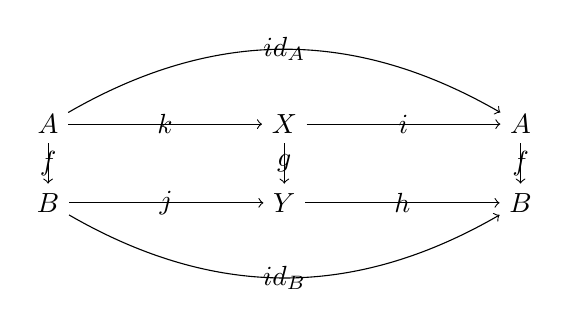
\begin{tikzpicture}
	\node (1) {$A$};
	\node (2) [below of=1] {$B$};
	\node (3) [node distance=3cm, right of=1] {$X$};
	\node (4) [below of=3] {$Y$};
	\node (5) [node distance=3cm, right of=3]{$A$};
	\node (6) [below of=5] {$B$};
	
	\draw [-to] (1) to node [swap]{$f$} (2);
	\draw [-to] (1) to node [swap]{$k$} (3);
	\draw [-to] (2) to node {$j$} (4);
	\draw [-to] (3) to node {$g$} (4);
	\draw [-to] (5) to node {$f$} (6);
	\draw [-to] (4) to node {$h$} (6);
	\draw [-to] (3) to node [swap]{$i$} (5);
	\draw [-to, bend left] (1) to node {$id_A$} (5);
	\draw [-to, bend right] (2) to node [swap] {$id_B$} (6);	
\end{tikzpicture}
\end{center}
such that the horizontal maps compose to the identity. 
\end{definition}

\begin{definition}[Retraction closed]
\label{def:retraction_closed}
\index{Retraction closed}
A class of morphisms $R$ is called retraction closed if every retraction of a morphism in $R$ is again in $R$. 
\end{definition}

Note that if a retraction closed class contains all the identitiy morphism, then it must contain all isomophims as well. 



\begin{definition}[Model structure]
\label{def:model_structure}
\index{Model structure}
Let $\mathcal{C}$ be a category. A model structure on $\mathcal{C}$ is a choice of three distinguished collections of maps, $F$, $C$ and $W$, in $\mathcal{C}$
such that the axioms below hold. The maps in the collections are called \emph{fibrations}\index{Fibration}, \emph{cofibrations}\index{Cofibration} and \emph{weak equivalences}\index{Weak equivalence} respectively, and maps in $F\cap W$ are called \emph{acyclic fibrations}\index{Acyclic fibration} and maps in $C\cap W$ are called \emph{acyclic cofibrations}\index{Acyclic cofibration}. The axioms are:

\textbf{MC1:}
Any retraction of a map in one of the three classes is again in the same class, i.e. all three classes are retraction closed. 

\textbf{MC2:}
The collection $W$ of weak equivalences has the two out of three property, i.e. if two out of $f, g, g\circ f$ is a weak equivalence, then the third is as well.

\textbf{MC3:}
If we have a commutative square 

\begin{center}
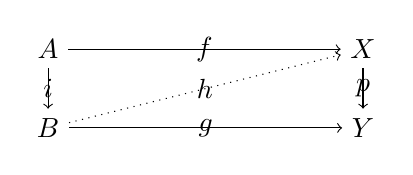
\begin{tikzpicture}
	\node (1) {$A$};
	\node (3) [below of=1] {$B$};
	\node (2) [node distance=4cm, right of=1] {$X$};
	\node (4) [below of=2] {$Y$};

	\draw [-to] (1) to node {$f$} (2);
	\draw [-to] (1) to node [swap]{$i$} (3);
	\draw [-to] (2) to node {$p$} (4);
	\draw [-to] (3) to node [swap]{$g$} (4);	
	\draw [-to, dotted] (3) to node {$h$} (2);
\end{tikzpicture}
\end{center}

where either $i\in C$ and $p\in F\cap W$, or $i\in C\cap W$ and $p\in F$, then there exists a lift $h$ making both subdiagrams commute.

\textbf{MC4:}
Given any map $f:X\longrightarrow Y$ in $\mathcal{C}$ we can factor it as $f=p\circ i$, where $p\in F$ and $i\in C\cap W$ and as $f=p'\circ i'$ where $i'\in C$ and $p'\in F\cap W$. 
\end{definition}

We then define a \emph{model category}\index{Model category} to be a bicomplete category---a category where all small limits and colimits exists---with a model structure. 

The two parts in \textbf{MC3} are often stated as fibrations having \emph{the right lifting property}\index{Right lifting property} with respect to acyclic cofibrations, and cofibrations having \emph{the left lifting property}\index{Left lifting property} with respect to acyclic fibrations. 


The archetypal example of a model category is the category of topological spaces. This category has two often used model structures, often called the Quillen (or Serre) model structure and the Strøm model structure. 

\begin{example}[Quillen model structure on topological spaces]
\label{ex:quillen_model}
The underlying category is the category of topological spaces with continuous maps. The fibrations consists of the Serre fibrations, which are maps that have the so called homotopy lifting property with respect to all CW complexes. This property is described by lifts $h$ existing when we have a CW complex $X$, and a diagram
\begin{center}
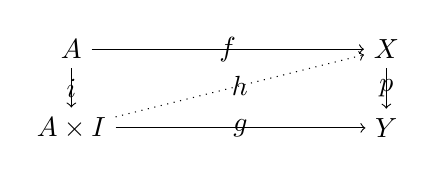
\begin{tikzpicture}
	\node (1) {$A$};
	\node (3) [below of=1] {$A\times I$};
	\node (2) [node distance=4cm, right of=1] {$X$};
	\node (4) [below of=2] {$Y$};

	\draw [-to] (1) to node {$f$} (2);
	\draw [-to] (1) to node [swap]{$i$} (3);
	\draw [-to] (2) to node {$p$} (4);
	\draw [-to] (3) to node [swap]{$g$} (4);	
	\draw [-to, dotted] (3) to node {$h$} (2);
\end{tikzpicture}
\end{center}
where $I$ is the unit interval and $i_0:A\longrightarrow A\times I$ is the inclusion into the first component. 

The cofibrations are defined by being induced by retracts of relative CW complexes, i.e. maps $g:X\longrightarrow Y$ where $Y$ is made from $X$ by attaching cells. The weak equivalences are weak homotopy equivalences, which are maps that induce isomorphisms on all homotopy groups. 
\end{example}

\begin{example}[Strøm model structure on topological spaces]
\label{ex:strom_model}
As with the previous example, the category of interest is the category of topological spaces with continuous maps. The fibrations are the Hurewicz fibrations, which satisfies the homotopy lifting property with respect to all topological spaces, not just the CW complexes as the Serre fibrations. The cofibrations are the closed Hurewicz cofibrations, which satisfy the homotopy extension property. This property is described by a lift $h$ existing when the diagram below commutes.

\begin{center}
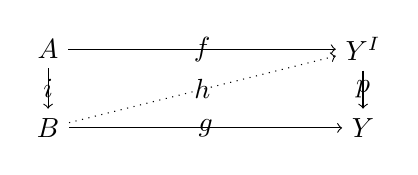
\begin{tikzpicture}
	\node (1) {$A$};
	\node (3) [below of=1] {$B$};
	\node (2) [node distance=4cm, right of=1] {$Y^I$};
	\node (4) [below of=2] {$Y$};

	\draw [-to] (1) to node {$f$} (2);
	\draw [-to] (1) to node [swap]{$i$} (3);
	\draw [-to] (2) to node {$p$} (4);
	\draw [-to] (3) to node [swap]{$g$} (4);	
	\draw [-to, dotted] (3) to node {$h$} (2);
\end{tikzpicture}
\end{center}

Here $Y^I$ is the path space of $Y$ and $p$ is the projection onto the start of a path. We call a map $i:A\longrightarrow B$ satisfying this property a Hurewicz cofibration, and we say it is a closed Hurewicz cofibration if its image is closed in $B$. The weak equivalences are given by the homotopy equivalences, i.e. the maps that are invertible up to homotopy.  
\end{example}

\begin{example}
\label{ex:cochain_complexes}
Another example is the category of positively graded cochain complexes of modules over a ring, $Ch(R-mod)$. Here the model structure consists of quasi-isomorphisms as the weak equivalences, the fibrations are degreewise projections and the cofibrations are degreewise injections with projective cokernel. The homotopy theory we get in this setting is the theory of homological algebra. 

We can expand use a similar definition for unbounded chain complexes, but then the cofibrations need a bit more care. They can however easily be defined as the morphisms that have the left lifting property with respect to the acyclic fibrations. This model category also motivates how we will define the model structure on DG-algebras, as DG-algebras are unbounded chain complexes. We can actually construct the model category of DG-algebras directly from the model category of unbounded chain complexes of vector spaces, as done in \cref{ap:A}. 
\end{example}


\subsection{Constructions in model categories}

We said that model structures allows us to introduce the notion of homotopy into the category. We will now see this construction, but first we introduce the definition of the homotopy category. Rather surprisingly, and unintuitively, this seemingly has nothing to do with homotopies at all---at least not yet. 

\begin{definition}[The homotopy category]
\label{def:homotopy_category}
\index{The homotopy category}
Let $\mathcal{C}$ be a model category and $W$ its collection of weak equivalences. We define the homotopy category of $\mathcal{C}$ to be the category $Ho\mathcal{C} = \mathcal{C}[W^{-1}]$, i.e. the localization at the weak equivalences. 
\end{definition}

\begin{remark}
The readers familiar with homological algebra will hopefully see some similarities to derived categories of rings. These are defined by localizing the category of cochain complexes of modules at the quasi-isomorphisms, which we just saw formed the weak equivalences in \cref{ex:cochain_complexes}. 
\end{remark}

Since a model category is bicomplete, it has both an \emph{initial object}\index{Initial object} $I$ and a \emph{terminal object}\index{Terminal object} $T$. Recall that these are objects where there exists a unique map from and to any other object in the category respectively. 

\begin{definition}[Fibrant object]
\label{def:fibrant}
\index{Fibrant object}
Let $X$ be an object in a model category $\mathcal{C}$. We say $X$ is fibrant if the unique map $X\longrightarrow T$ is a fibration. 
\end{definition}

\begin{definition}[Cofibrant object]
\label{def:cofibrant}
\index{Cofibrant object}
Let $X$ be an object in a model category $\mathcal{C}$. We say $X$ is cofibrant if the unique map $I\longrightarrow X$ is a cofibration. 
\end{definition}

If $X$ is both fibrant and cofibrant, we reffer to it as \emph{bifibrant}\index{Bifibrant object}. 



\begin{definition}[Cylinder object]
\label{def:cylinder_object}
\index{Cylinder object}
Let $X$ be an object in a model category $\mathcal{C}$. The cylinder object of $X$, usually denoted $Cyl(X)$, is a factorization of the codiagonal map $\nabla: X\coprod X\longrightarrow X$ into
\begin{equation*}
    X\coprod X\overset{i_0+i_1}\longrightarrow Cyl(X) \overset{p}\longrightarrow X,
\end{equation*} 
where $p$ is a weak equivalence. 

If $X\coprod X\overset{i_1 + i_2}\rightarrow Cyl(X)$ is a cofibration, we call $Cyl(X)$ a \emph{good cylinder object}\index{Good cylinder object}, and if in addition $p$ is an acyclic fibration, we call $Cyl(X)$ a \emph{very good cylinder object}\index{Very good cylinder object}.
\end{definition}

\begin{definition}[Path object]
\label{def:path_object}
\index{Path object}
Given an object $X$ in a model category $\mathcal{C}$ we define the path object of $X$, denoted $Path(X)$ to be factorization of the diagonal map $\Delta\colon X \rightarrow X\prod X$ into
\begin{equation*}
     X \overset{i}\rightarrow Path(X) \overset{(p_1,p_2)}\rightarrow X \prod X,
\end{equation*}
where $i$ is a weak equivalence. Similarly to the cylinder object, if $Path(X)\overset{p}\rightarrow X\prod X$ is a fibration, we call $Path(X)$ a \emph{good path object}\index{Good path object}, and if in addition $i$ is an acyclic cobfiration, we call $Path(X)$ a \emph{very good path object}\index{Very good path object}.
\end{definition}

By the factorization axiom (\textbf{MC4}) every object has at least one very good cylinder object and one very good path object. It can be useful to use these in some cases, but in other cases we can actually be interested in cylinder and path objects that aren't necessarily good, or very good. For example, in the Serre model structure on topological spaces, the standard cylinder object $Cyl(X)=X\times I$ is only a good cylinder object when $X$ is a CW complex. It would sometimes be limiting to not use this standard cylinder when working with homotopies of maps between spaces that are not CW complexes, hence the reason for the weaker definition. 

Speaking of homotopies, we now have objects that resemble what we use in the category of topological spaces to define homotopies between maps. We should then be able to define them in any model category $\C$ as well. When we define homotopies in topology, we define them as maps from the cylinder $I\times X$ such that the restriction to the boundary of the cylinder gives us the two maps we are constructing a homotopy between. This is also what motivates how we define it in the general setting for model categories, but we need to be a bit more careful. For the below definitions we assume that all objects and all morphisms lie in som model category $\C$.

\begin{definition}[Left homotopy]
\label{def:left_homotopy}
\index{Left homotopy}
Given two maps $f,g: X\rightarrow Y$ we define a left homotopy $h:f\sim_L g$ from $f$ to $g$ to be a map $h: Cyl(X)\rightarrow Y$ such that the following diagram commutes
\begin{center}
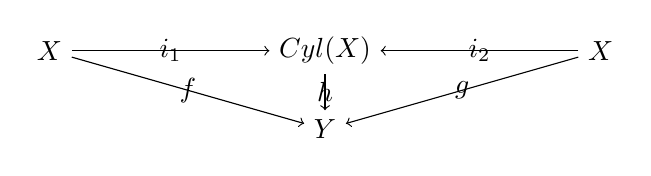
\begin{tikzpicture}
	\node (X) {$X$};
	\node (C) [node distance=3.5cm, right of=X] {$Cyl(X)$};
	\node (X') [node distance=3.5cm, right of=C] {$X$};
	\node (Y) [below of=C] {$Y$};

	\draw [-to] (X) to node {$i_1$} (C);
	\draw [-to] (X') to node [swap]{$i_2$} (C);
	\draw [-to] (X) to node [swap]{$f$} (Y);
	\draw [-to] (X') to node {$g$} (Y);
	\draw [-to] (C) to node {$h$} (Y);
\end{tikzpicture}
\end{center}
\end{definition}

\begin{definition}[Right homotopy]
\label{def:right_homotopy}
\index{Right homotopy}
Given two maps $f,g: X\rightarrow Y$ we define a right homotopy $h:f\sim_R g$ from $f$ to $g$ to be a map $h: X\rightarrow Path(Y)$ such that the following diagram commutes
\begin{center}
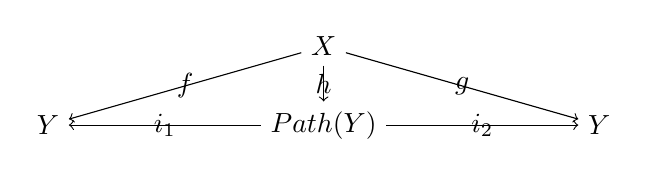
\begin{tikzpicture}
	\node (Y) {$Y$};
	\node (P) [node distance=3.5cm, right of=Y] {$Path(Y)$};
	\node (Y') [node distance=3.5cm, right of=P] {$Y$};
	\node (X) [above of=P] {$X$};

	\draw [-to] (X) to node [swap]{$f$} (Y);
	\draw [-to] (X) to node {$g$} (Y');
	\draw [-to] (X) to node {$h$} (P);
	\draw [-to] (P) to node {$i_1$} (Y);
	\draw [-to] (P) to node [swap]{$i_2$} (Y');
\end{tikzpicture}
\end{center}
\end{definition}

If the cylinder object used to define the left homotopy is a good cylinder object then we call the homotopy a \emph{good left homotopy}\index{Good left homotopy}, and similarly if it is a very good cylinder object we call the homotopy a \emph{very good left homotopy}\index{Very good left homotopy}. The same goes for the path object used to define the right homotopy, which gives us \emph{good right homotopies}\index{Good right homotopy} and \emph{very good right homotopies}\index{Very good right homotopy}.

The fact that homotopy is an equivalence relation on classes of continuous maps is one of the most important, and fundamental properties, that homotopy has in the category of topological spaces. Thus it should also be important in the general setting. Before we do that, we note that we can upgrade any left homotopy $h$ to a good left homotopy by factoring the map $X\rightarrow Cyl(X)$ into $X\rightarrow Cyl(X)' \overset{\sigma}\rightarrow Cyl(X)$ by \textbf{MC4}. Then $h\circ \sigma$ will be a good homotopy. If $Y$ is fibrant, then we can upgrade it further to a very good left homotopy by using the other factorization on $Cyl(X)\rightarrow Y$ to get $Cyl(X)\rightarrow Cyl(X)'\rightarrow Y$. This factorization gives us a commutative diagram
\begin{center}
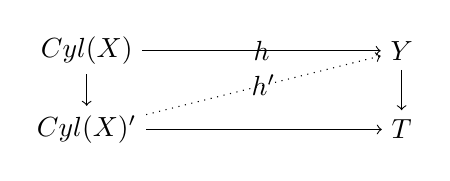
\begin{tikzpicture}
	\node (C) {$Cyl(X)$};
	\node (C') [below of=C] {$Cyl(X)'$};
	\node (Y) [node distance=4cm, right of=C] {$Y$};
	\node (T) [below of=Y] {$T$};

	\draw [-to] (C) to node {$h$} (Y);
	\draw [-to] (C) to node {} (C');
	\draw [-to] (C') to node {} (T);
	\draw [-to] (Y) to node {} (T);	
	\draw [-to, dotted] (C') to node {$h'$} (Y);
\end{tikzpicture}
\end{center}
where $T$ is the terminal object. The lift $h'$ comes from \textbf{MC3} and gives us the very good left homotopy that we wanted. 

\begin{lemma}
Let $X$ and $Y$ be objects in a model category $\mathcal{C}$. If $X$ is cofibrant then left homotopy defines an equivalence relation on $Hom(X,Y)$.
\end{lemma}
\begin{proof}
Using $X$ itself as a cylinder object together with the map $f:Cyl(X)=X\rightarrow Y$ as a left homotopy shows that any map $f:X\rightarrow Y$ is left homotopic to itself. It is symmetric---as we can compose with the switching map $X\coprod X \rightarrow X\coprod X$---that just switches the components. This gives a homotopy “in the other direction”. Lastly, let $f_1\sim_L f_2$ and $f_2\sim_L f_3$ be good homotopies with cylinder objects being $Cyl(X)$ and $Cyl(X)'$ respectively. Then the pushout of the diagram $Cyl(X)' \leftarrow X \rightarrow Cyl(X)$ defines a new cylinder object and a homotopy $f_1\sim f_3$. Hence the relation is reflexive, symmetric and transitive which is the definition of an equivalence relation.
\end{proof}

Dually, we also get the exact same result for right homotopy, but we have to switch from $X$ being cofibrant to $Y$ being fibrant. This is because from a model structure on a category $\mathcal{C}$ we also get a model structure on its opposite category. Here the classes of fibrations and cofibrations are switched, but the weak equivalences stay the same. 

It might feel uneasing that we now have two different concepts of homotopy, which we usually don't have when working in topological spaces. There is a good reason for this, because in both the Serre and the Strøm model structure on topological spaces, all objects are fibrant. Hence, by the next lemma, the existence of right homotopies always implies the existence of left homotopies in the category of topological spaces, which means we don’t ever need to make the distinction between them.

\begin{lemma}
Let $f,g:X\rightarrow Y$ be two maps. If $X$ is cofibrant and $f,g$ are left homotopic then they are right homotopic. Dually, if $Y$ is fibrant and $f,g$ are right homotopic, then they are left homotopic.
\end{lemma}
\begin{proof}
Choose a good cylinder object $X\coprod X \overset{i_1 + i_2}\rightarrow Cyl(X) \overset{j}\rightarrow X$ and let $h:Cyl(X)\rightarrow Y$ be a left homotopy between $f$ and $g$. Choose also a good path object $Y\overset{q}\rightarrow Path(Y) \overset{(p_1, p_2)}\rightarrow Y\prod Y$. We then have a commutative diagram
\begin{center}
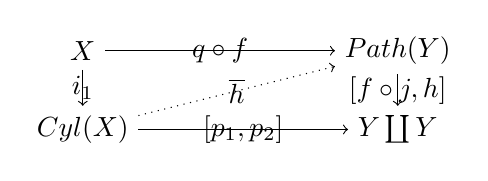
\begin{tikzpicture}
	\node (X) {$X$};
	\node (C) [below of=X] {$Cyl(X)$};
	\node (P) [node distance=4cm, right of=X] {$Path(Y)$};
	\node (Y) [below of=P] {$Y\coprod Y$};

	\draw [-to] (X) to node {$q\circ f$} (P);
	\draw [-to] (X) to node [swap]{$i_1$} (C);
	\draw [-to] (C) to node [swap]{$[p_1, p_2]$} (Y);
	\draw [-to] (P) to node {$[f\circ j, h]$} (Y);	
	\draw [-to, dotted] (C) to node {$\overline{h}$} (P);
\end{tikzpicture}
\end{center}
which has a lift $\overline{h}$ by \textbf{MC3}. 
%Note here that we used the fact that $i_1$ is an acyclic cofibration which we have not proved, but it can be seen by the two out of three property since $X$ is assumed to be cofibrant together with the fact that it is a composition of two cofibrations. 
The composition $h\circ i_2:X\rightarrow Path(X)$ gives a right homotopy between $f$ and $g$ as desired. The dual statement is proved dually.
\end{proof}

We can then finally define the notion of homotopy as follows. 

\begin{definition}[Homtopic maps]
\label{def:homotopic_maps}
\index{Homotopic maps}
We say two maps $f,g:X\rightarrow Y$ are homotopic, denoted $f\sim g$, if they are both left homotopic and right homotopic.
\end{definition}

This means we can finally define homotopy equivalences. 

\begin{definition}[Homotopy equivalence]
\label{def:homotopy_equivalence}
\index{Homotopy equivalence}
We say a morphism $f\colon X\longrightarrow Y$ is a homotopy equivalence if there exists a morphism $g\colon Y\longrightarrow Y$ such that $f\circ g \sim id_Y$ and $g\circ f \sim id_X$. If there exists a homotopy equivalence between two objects, we call them homotopy equivalent.
\end{definition}

If we now restrict our attention to just the bifibrant\index{Bifibrant object} objects in a model category, we see that we have a well defined notion of homotopy. It is well defined in the sense that it is an equivalence relation. A question we could ask is: when are two objects are homotopy equivalent? and how does this notion of homotopy equivalence relate to weak equivalences? We have a very nice correspondence in this setting, i.e. when restricting to the bifibrant objects. 

\begin{theorem}[Generalized Whiteheads theorem]
\label{thm:whitehead}
\index{Generalized Whiteheads theorem}
Two bifibrant objects $X$ and $Y$, in a model category $\C$, are homotopy equivalent if and only if they are weakly equivalent. 
\end{theorem}

We won't cover the proof, but refer to \cite[Theorem 1.2.10.]{hovey}. 

This means that localizing at the weak equivalences also turns homotopy equivalences of bifibrant objects into isomorphisms. If we take the subcategory of bifibrant objects, which we denote $\C_{cf}$, we can form its quotient by the homotopy relation, $\C_{cf}\longrightarrow \C_{cf}/\sim$. By the generalized Whitehead theorem this map sends weak equivalences to isomorphisms, and hence it has to factor through its homotopy category, $Ho(\C_{cf})$, by general theory about localization. We also have an inclusion $\C_{cf} \longrightarrow \C$ which induces a map on their homotopy categories, $Ho(\C_{cf})\rightarrow Ho(\C)$. The final piece of the puzzle of having a workable homotopy category, comes from the fact that those maps form an equivalence of categories $Ho(\C)\cong \C_{cf}/\sim$, which means that we have a nice definition, and a nice way to work with it.














\section{The homotopy theory of DG-algebras}

When lookin at some examples of model categories, we mentioned that the model structure on the category of DG-algebras would be similar to the model structure on chain complexes of modules over a ring. 

The model structure is constructed by Jardine in \cite{jardine} and is described by the weak equivalences being the quasi-isomorphisms, the fibrations being the degreewise surjections and the cofibrations being all maps that have the left lifting property with respect to acyclic fibrations. 

Lets prove that this is in fact a model structure on the category $DGA_k$ of DG-algebras over a field $k$. This construction and proof holds more generally for $k$ a commutative unital ring. Note that much of this proof is directly inspired by the  original paper \cite{jardine}, but we have tried to fill in some details, and prove some parts that is left out by Jardine. We will not prove that the second factorization in \textbf{MC4} holds in $DGA_k$, as it requires us to go into the so-called ``small objects argument''. For a proof of that result, see \cite[Theorem 2.1.14]{hovey}, and for a more in depth conceptual treatment, see \cite{small_objects}.

To help us with some of the proofs of the different axioms we let:
\begin{itemize}
	\item $S(x)$ be the free graded $k$-algebra on one generator $x$ in degree $n$ together with the differential defined by $d(x)=0$.
	
	\item $T(x)$ be the free graded $k$-algebra on two generators, $x$ and $dx$, together with the differential defined by $d(x)=dx$ and $d(dx)=0$. This is the free DG-algebra on one generator.
	\item $C(x)$ be the free cochain complex on one generator $x$ in degree $n$, i.e. the complex 
\begin{equation*}
    C(x)^i = 
    \begin{cases}
        &  0, i\neq n, i\neq n+1 \\
        & k, i = n, i= n+1
    \end{cases}
\end{equation*}
where the differential is trivial, except for being the identity on $k$ in degree $n$. 
\end{itemize}


The coproduct of two DG-algebras $A$ and $B$ is defined by $A\ast B = T(A\otimes B)/I$, where $T(A\otimes B)$ is the tensor algebra
\begin{equation*}
    T(A\otimes B) = \bigoplus_{n \in \N}(A\otimes B)^{\otimes n}
\end{equation*}
and $I$ is the ideal generated by 
\begin{equation*}
    \begin{cases}
        & (a\otimes b_1)\otimes (1\otimes b_2) - a\otimes b_1 b_2    \\
        & (a_1\otimes 1)\otimes (a_2 \otimes b) - a_1 a_2 \otimes b
    \end{cases}
\end{equation*}

Note that we can identify $T(x)$ with the tensor algebra on $C(x)$, i.e. 
\begin{equation*}
    T(x) \overset{\cong}\longrightarrow T(C(x)) = \bigoplus_{i\geq 0}C(x)^{\otimes i}
\end{equation*}

Hence we have 
\begin{equation*}
H^i(T(x)) = 
\begin{cases}
    &k, i=0 \\
    &0, else
\end{cases}
\end{equation*}

\begin{definition}
Let $A$ be a DG-algebra and $C$ a cochain complex. We define the DG-algebra $A[C]$ to be the cochain complex
\begin{equation*}
    A[C] = A\oplus (A\otimes C\otimes A) \oplus (A\otimes C \otimes A \otimes C \otimes A) \oplus \cdots
\end{equation*}
together with multiplication defined by 
\begin{equation*}
    (a_1\otimes b_1 \otimes \cdots \otimes b_k \otimes a_{k+1}) \cdot (a'_1\otimes b'_1 \otimes \cdots \otimes b'_l \otimes a'_{l+1}) = a_1 \otimes \cdots \otimes b_k \otimes a_{k+1}a'_1 \otimes \cdots \otimes b'_l \otimes a'_{l+1}
\end{equation*}
\end{definition}

Any map from this DG-algebra $f:A[C]\longrightarrow B$ is uniquely determined by its restriction to its first component $A$ and the chain map on the first occurring $C$, i.e. the map $j_f$ defined by by the composition
\begin{equation*}
    j_f: C\overset{inc}\longrightarrow A\otimes C\otimes A \subseteq A[C]\overset{f}\longrightarrow B
\end{equation*}
where $inc(c) = 1\otimes c \otimes 1$. 

Hence we have an isomorphism $A\ast_k T(x) \cong A[C(X)]$ from the coproduct to this ``free algebra'' on $C$. This is because $T(x)\cong T(C(x))$, and the map $A[C(x)]\rightarrow A\ast_k T(C(x))$ is uniquely determined by sending $A$ into $A$, and $C(x)$ into $C(x)$ as a component of $T(C(x))$. 


\begin{lemma}
The map $k\longrightarrow T(x)$ is a cofibration. 
\end{lemma}
\begin{proof}
    We need to show that a lift $h:T(X)\longrightarrow A$ exists for all commuting diagrams
\begin{center}
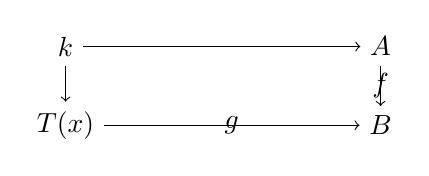
\begin{tikzpicture}
	\node (1) {$k$};
	\node (2) [below of=1] {$T(x)$};
	\node (3) [node distance=4cm, right of=1] {$A$};
	\node (4) [below of=3] {$B$};

	\draw [-to] (1) to node {} (2);
	\draw [-to] (1) to node {} (3);
	\draw [-to] (2) to node [swap]{$g$} (4);
	\draw [-to] (3) to node {$f$} (4);	
\end{tikzpicture}
\end{center}
    
The push-out of the diagram 
\begin{center}
\begin{tikzpicture}
	\node (1) {$k$};
	\node (2) [below of=1] {$T(x)$};
	\node (3) [node distance=4cm, right of=1] {$A$};

	\draw [-to] (1) to node {} (2);
	\draw [-to] (1) to node {} (3);
\end{tikzpicture}
\end{center}
is the coproduct $A\ast_k T(x)$, which we know is isomorphic to $A[C(x)]$. Hence we have a unique map $B\longrightarrow A[C(x)]$ by the universal property of a push-out, i.e. 
\begin{center}
\begin{tikzpicture}
	\node (1) {$k$};
	\node (2) [below of=1] {$T(x)$};
	\node (3) [node distance=4cm, right of=1] {$A$};
	\node (4) [below of=3] {$B$};
	\node (5) [node distance=2cm, right of=4, below of=4] {$A[C(x)]$};

	\draw [-to] (1) to node {} (2);
	\draw [-to] (1) to node {} (3);
	\draw [-to] (2) to node [swap]{$g$} (4);
	\draw [-to] (3) to node {$f$} (4);	
	\draw [-to, dotted] (4) to node {$\phi$} (5);
	\draw [-to, bend left] (3) to node {} (5);
	\draw [-to, bend right] (2) to node {} (5);
\end{tikzpicture}
\end{center}
We can then define the map $h = p_A \circ \phi \circ g$, where $p_A$ is the projection onto the first component, which is uniquely determined by being the identity on $A$ and $j_{p_A} = 0$. 
    
Then the diagram 
\begin{center}
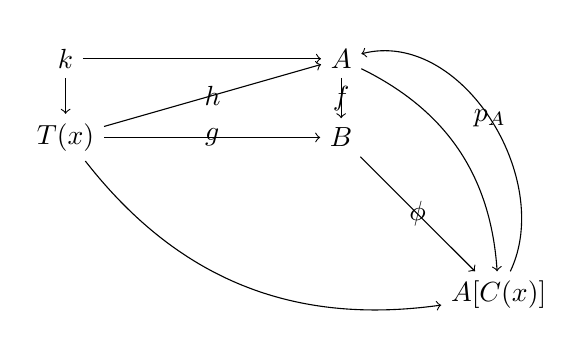
\begin{tikzpicture}
	\node (1) {$k$};
	\node (2) [below of=1] {$T(x)$};
	\node (3) [node distance=3.5cm, right of=1] {$A$};
	\node (4) [below of=3] {$B$};
	\node (5) [node distance=2cm, right of=4, below of=4] {$A[C(x)]$};

	\draw [-to] (1) to node {} (2);
	\draw [-to] (1) to node {} (3);
	\draw [-to] (2) to node [swap]{$g$} (4);
	\draw [-to] (3) to node {$f$} (4);	
	\draw [-to] (2) to node {$h$} (3);
	\draw [-to] (4) to node {$\phi$} (5);
	\draw [-to, bend left] (3) to node {} (5);
	\draw [-to, bend right] (2) to node {} (5);
	\draw [-to, bend right, in=250, out=300] (5) to node [swap]{$p_A$} (3);
\end{tikzpicture}
\end{center}
commutes everywhere, and we are done. 
\end{proof}




\begin{theorem}
The category $DGA_k$ of DG-algebras over a field $k$, together with the three classes of morphisms; $W$, $C$, $F$, as described above, form a model category.
\end{theorem}

\begin{proof}
We need to check the four axioms. 

\textbf{MC 1:} This point consists of three sub-points. We first prove that $F$ is retraction closed, then $W$ and finally $C$. 

Assume $f:A\longrightarrow B$ is a retract of $g:X\longrightarrow Y$ where $g\in F$. This means we have a diagram

\begin{center}
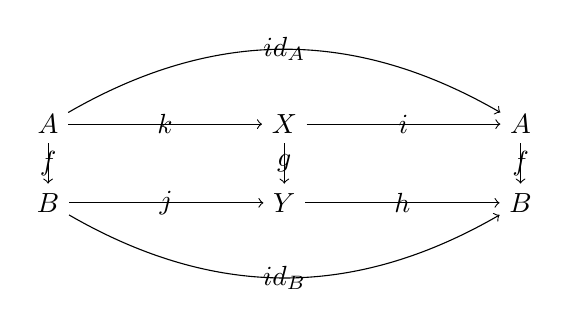
\begin{tikzpicture}
	\node (1) {$A$};
	\node (2) [below of=1] {$B$};
	\node (3) [node distance=3cm, right of=1] {$X$};
	\node (4) [below of=3] {$Y$};
	\node (5) [node distance=3cm, right of=3]{$A$};
	\node (6) [below of=5] {$B$};
	
	\draw [-to] (1) to node [swap]{$f$} (2);
	\draw [-to] (1) to node [swap]{$k$} (3);
	\draw [-to] (2) to node {$j$} (4);
	\draw [-to] (3) to node {$g$} (4);
	\draw [-to] (5) to node {$f$} (6);
	\draw [-to] (4) to node {$h$} (6);
	\draw [-to] (3) to node [swap]{$i$} (5);
	\draw [-to, bend left] (1) to node {$id_A$} (5);
	\draw [-to, bend right] (2) to node [swap] {$id_B$} (6);	
\end{tikzpicture}
\end{center}

Let $b$ be a homogeneous element in degree $n$. Want to show that there is a homogeneous element $a$ such that $f(a)=b$, as this would show that $f$ is degree-wise surjective, i.e. $f\in F$. 
    
Let $y = j(b)$. Since $g\in F$ it is a degree-wise surjection and hence there exists an element $x\in X$ such that $g(x)=y$. Let $i(x)=a$. Then we have 
\begin{align*}
    f(a) 
    &= f(i(x) \\
    &= h(g(x)) \\
    &= h(j(b)) \\
    &= id_B(b) = b.
\end{align*}
which shows that the retract of a fibration is again a fibration. 

For the second part we let $g\in W$ and $f$ still a retraction of $g$. We have the same retraction diagram as above, which induces the following diagram in cohomology:
\begin{center}
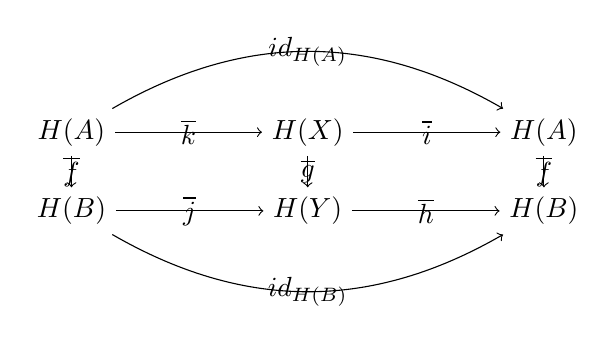
\begin{tikzpicture}
	\node (1) {$H(A)$};
	\node (2) [below of=1] {$H(B)$};
	\node (3) [node distance=3cm, right of=1] {$H(X)$};
	\node (4) [below of=3] {$H(Y)$};
	\node (5) [node distance=3cm, right of=3]{$H(A)$};
	\node (6) [below of=5] {$H(B)$};
	
	\draw [-to] (1) to node [swap]{$\overline{f}$} (2);
	\draw [-to] (1) to node [swap]{$\overline{k}$} (3);
	\draw [-to] (2) to node {$\overline{j}$} (4);
	\draw [-to] (3) to node {$\overline{g}$} (4);
	\draw [-to] (5) to node {$\overline{f}$} (6);
	\draw [-to] (4) to node {$\overline{h}$} (6);
	\draw [-to] (3) to node [swap]{$\overline{i}$} (5);
	\draw [-to, bend left] (1) to node {$id_{H(A)}$} (5);
	\draw [-to, bend right] (2) to node [swap] {$id_{H(B)}$} (6);	
\end{tikzpicture}
\end{center}

Recall that we want to show that $f$ induced an isomorphism in cohomology. As $g$ is surjective, we can use the same argument as above---when we had $f\in F$---to get that $\overline{f}$ is surjective. Assume now that $\overline{f}([a]) = \overline{f}([a'])$. Then $\overline{j}(\overline{f}([a])) = \overline{j}(\overline{f}([a']))$, which means $\overline{g}(\overline{k}([a])) = \overline{g}(\overline{k}([a']))$. But $\overline{g}$ is an isomorphism, and hence we have $\overline{k}([a]) = \overline{k}([a'])$ and finally
\begin{equation*}
    [a] = id_A([a]) = \overline{i}(\overline{k}([a])) = \overline{i}(\overline{k}([a'])) = id_A([a']) = [a']
\end{equation*}
This shows that $\overline{f}$ is both injectiv and surjective, i.e. an isomorphism---which means that $f\in W$. 

For the last part we let $g\in C$, and $f$ still a retraction of $g$. Recall that we need to have a lift of $f$ with respect to all acyclic fibrations $[p\colon U\longrightarrow V]\in F\cap W$, i.e. the existence of the dotted morphism $\phi$ in the following diagram
\begin{center}
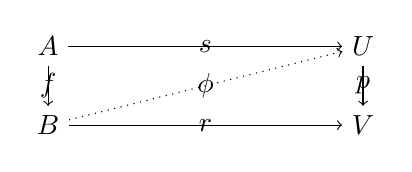
\begin{tikzpicture}
	\node (1) {$A$};
	\node (2) [node distance=4cm, right of=1] {$U$};
	\node (3) [below of=1] {$B$};
	\node (4) [below of=2] {$V$};

	\draw [-to] (1) to node {$s$} (2);
	\draw [-to] (1) to node [swap]{$f$} (3);
	\draw [-to] (2) to node {$p$} (4);
	\draw [-to] (3) to node [swap]{$r$} (4);	
	\draw [-to, dotted] (3) to node {$\phi$} (2);
\end{tikzpicture}
\end{center}

We get this by producing a lift from $g$, as it is in $C$. As $f$ is a retraction of $f$ we can extend the above diagram to 
\begin{center}
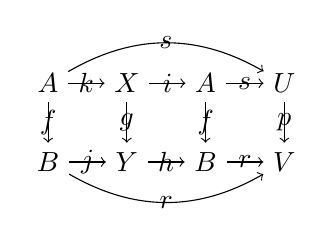
\begin{tikzpicture}
	\node (1) {$A$};
	\node (2) [right of=1] {$X$};	
	\node (3) [right of=2]{$A$};	
	\node (4) [right of=3] {$U$};	
	
	\node (5) [below of=1] {$B$};
	\node (6) [below of=2] {$Y$};
	\node (7) [below of=3] {$B$};
	\node (8) [below of=4] {$V$};
	
	\draw [-to] (1) to node [swap]{$f$} (5);
	\draw [-to] (1) to node [swap]{$k$} (2);
	\draw [-to] (5) to node {$j$} (6);
	\draw [-to] (2) to node {$g$} (6);
	\draw [-to] (3) to node {$f$} (7);
	\draw [-to] (6) to node {$h$} (7);
	\draw [-to] (2) to node [swap]{$i$} (3);
	\draw [-to] (3) to node [swap]{$s$} (4);
	\draw [-to] (7) to node {$r$} (8);	
	\draw [-to] (4) to node {$p$} (8);	
	\draw [-to, bend left] (1) to node {$s$} (4);
	\draw [-to, bend right] (5) to node [swap]{$r$} (8);	
\end{tikzpicture}
\end{center}

This diagram has the sub-diagram  
\begin{center}
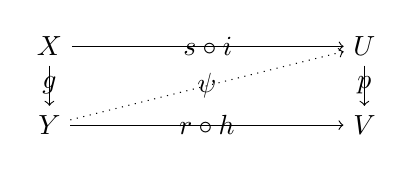
\begin{tikzpicture}
	\node (1) {$X$};
	\node (2) [node distance=4cm, right of=1] {$U$};
	\node (3) [below of=1] {$Y$};
	\node (4) [below of=2] {$V$};

	\draw [-to] (1) to node {$s\circ i$} (2);
	\draw [-to] (1) to node [swap]{$g$} (3);
	\draw [-to] (2) to node {$p$} (4);
	\draw [-to] (3) to node [swap]{$r\circ h$} (4);	
	\draw [-to, dotted] (3) to node {$\psi$} (2);
\end{tikzpicture}
\end{center}
where we know that the lift $\psi$, exists, as $g\in C$ and $p\in F\cap W$. We can then define $\psi = \psi\circ j$, i.e. the dotted arrow in the following diagram
\begin{center}
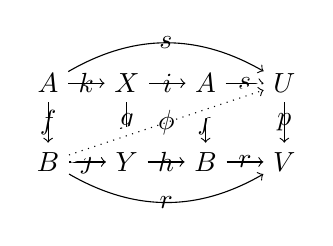
\begin{tikzpicture}[%
	cross line/.style={preaction={draw=white, -,line width=6pt}}]
	\node (1) {$A$};
	\node (2) [right of=1] {$X$};	
	\node (3) [right of=2]{$A$};	
	\node (4) [right of=3] {$U$};	
	
	\node (5) [below of=1] {$B$};
	\node (6) [below of=2] {$Y$};
	\node (7) [below of=3] {$B$};
	\node (8) [below of=4] {$V$};
	
	\draw [-to] (1) to node [swap]{$f$} (5);
	\draw [-to] (1) to node {$k$} (2);
	\draw [-to] (5) to node [swap]{$j$} (6);
	\draw [-to] (2) to node [swap]{$g$} (6);
	\draw [-to] (3) to node {$f$} (7);
	\draw [-to] (6) to node [swap]{$h$} (7);
	\draw [-to] (2) to node {$i$} (3);
	\draw [-to] (3) to node {$s$} (4);
	\draw [-to] (7) to node [swap]{$r$} (8);	
	\draw [-to] (4) to node {$p$} (8);	
	\draw [-to, bend left] (1) to node {$s$} (4);
	\draw [-to, bend right] (5) to node [swap]{$r$} (8);	
	\draw [-to, cross line, dotted] (5) to node {$\phi$} (4);
	
\end{tikzpicture}
\end{center}
Hence all retractions of morphisms in $C$ satisfy the lifting property with respect to morphisms in $F\cap W$, which means they are again in $C$. 


\textbf{MC 2:} Isomorphisms of DG-algebras have the two out of three property, and since quasi-isomorphisms are defined by inducing isomorphisms on the cohomology algebras, they also satisfy the property. 
    
\textbf{MC 3:} Notice that one half of this axiom holds by definition, as we defined cofibrations to be the morphisms that satisfied the left lifting property with respect to acyclic fibrations. For the other half we need to show that if we have a diagram 
\begin{center}
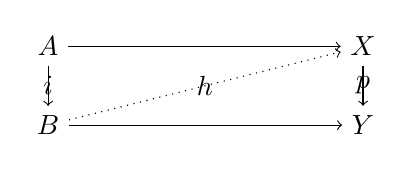
\begin{tikzpicture}
	\node (1) {$A$};
	\node (3) [below of=1] {$B$};
	\node (2) [node distance=4cm, right of=1] {$X$};
	\node (4) [below of=2] {$Y$};

	\draw [-to] (1) to node {} (2);
	\draw [-to] (1) to node [swap]{$i$} (3);
	\draw [-to] (2) to node {$p$} (4);
	\draw [-to] (3) to node [swap]{} (4);	
	\draw [-to, dotted] (3) to node {$h$} (2);
\end{tikzpicture}
\end{center}
where $i$ is an acyclic cofibration, and $p$ a fibration, then a lift exists. 
    
We can translate the problem to showing that every morphism $i\in C\cap W$ has the right lifting property w.r.t. all fibrations $p\in F$. 
    
Assume we have proven MC4, then we can factorize $i= f\circ j$ such that $j\in C\cap W$ and $f\in F$. Since two of them are in $W$ then the last one also is by MC2.

Hence we have a diagram 
\begin{center}
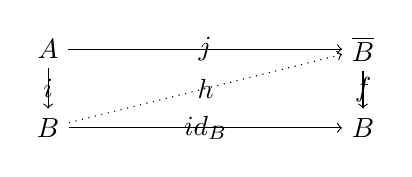
\begin{tikzpicture}
	\node (1) {$A$};
	\node (3) [below of=1] {$B$};
	\node (2) [node distance=4cm, right of=1] {$\overline{B}$};
	\node (4) [below of=2] {$B$};

	\draw [-to] (1) to node {$j$} (2);
	\draw [-to] (1) to node [swap]{$i$} (3);
	\draw [-to] (2) to node {$f$} (4);
	\draw [-to] (3) to node [swap]{$id_B$} (4);	
	\draw [-to, dotted] (3) to node {$h$} (2);
\end{tikzpicture}
\end{center}
    
that has a lift $h$ by the definition of $C$. 

By the commutativity of the previous diagram we have a new diagram 
\begin{center}
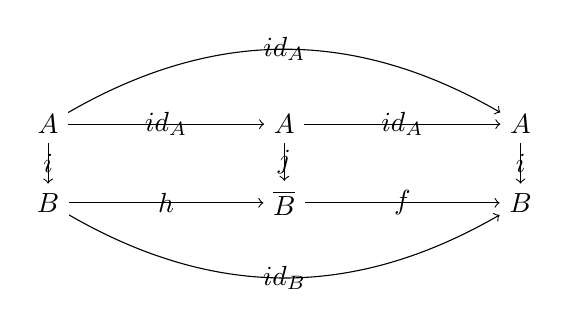
\begin{tikzpicture}
	\node (1) {$A$};
	\node (2) [below of=1] {$B$};
	\node (3) [node distance=3cm, right of=1] {$A$};
	\node (4) [below of=3] {$\overline{B}$};
	\node (5) [node distance=3cm, right of=3]{$A$};
	\node (6) [below of=5] {$B$};
	
	\draw [-to] (1) to node [swap]{$i$} (2);
	\draw [-to] (1) to node [swap]{$id_A$} (3);
	\draw [-to] (2) to node {$h$} (4);
	\draw [-to] (3) to node {$j$} (4);
	\draw [-to] (5) to node {$i$} (6);
	\draw [-to] (4) to node {$f$} (6);
	\draw [-to] (3) to node [swap]{$id_A$} (5);
	\draw [-to, bend left] (1) to node {$id_A$} (5);
	\draw [-to, bend right] (2) to node [swap] {$id_B$} (6);	
\end{tikzpicture}
\end{center}
which means that $i$ is a retraction of $j$, which we know has the right lifting property w.r.t all maps $f\in F$, hence $i$ does as well.



\textbf{MC 4:} Let $f:A\longrightarrow B$ be any map between two DG-algebras. We can form the factorization 
\begin{equation*}
    A\overset{i}\longrightarrow A\ast (\ast_{b\in B} T(B))\overset{p}\longrightarrow B
\end{equation*}
where $i$ is the inclusion and $p$ is the map that sends the generator $b \in T(B)$ to $b\in B$. The map $q$ is a fibration as it is  degreewise surjection, and the map $i$ is a filtered colimit of maps $A\longrightarrow T(b_1)\ast \cdots T(b_n)\ast A$ which all are acyclic cofibrations by iterating the construction of the isomorphism $T(x)\ast A \cong A[C(x)]$. Hence it is also itself an acyclic cofibration. 

The last factorization is as mentioned left out, due to us not covering the small objects argument in this thesis. See \cite[Lemma 3]{jardine} for a proof using this argument. 
\end{proof}


As we now know that $DGA_k$ is a model category, we know there exists a terminal and an initial object. In $DGA_k$ the terminal object is $0$---the complex consisting only of zeroes with only trivial differentials and trivial multiplication---while the initial object is the ground field $k$---treated as a DG-algebra by having only one copy of $k$ in degree zero and zeroes everywhere else. 

Since the unique map $0: A\longrightarrow 0$ is a degreewise surjection for any DG-algebra $A$ we know that all DG-algebras are fibrant objects in this model structure. 




\subsection{More formality}

This new framework allows us to reconsider the definition of a formal DG algebra. We take the category $DGA_k$, which we now know is a model category with $W$ being the collection of quasi-isomorphisms, and produce its homotopy category $HoDGA_k = DGA_k[W^{-1}]$. We can then define a DG algebra to be formal as follows. 

\begin{definition}[Formal DG-algebra]
A DG-algebra $(A, d)$ is called formal if it is isomorphic to its cohomology algebra $H(A)$ in $HoDGA_k$.
\end{definition}

This is the precise reason we referred to formal DG-algebras in the abstract as being the algebras that contain the same homotopical information as their cohomology algebra. They are isomorphic in the homotopy category, hence contain the same information up to homotopy. Such information is what we call homotopical information. 

Unfortunately not all isomorphisms in $HoDGA_k$ come from a single quasi-isomorphism in $DGA_k$. Quasi-isomorphisms in $DGA_k$ are not invertible, and not even homotopy invertible in general. Thus a zig-zag of quasi-isomorphisms is the best we can hope for, which means that this new definition is precisely the same as the old. 

A feature of this new framework is that we actually don't need an arbitrary zig-zag of quasi-isomorphisms, we only need a single span. To prove this we will need the following. 

\begin{definition}[Right proper model category]
Let $\C$ be a model category. We say it is right proper if the pullback of a weak equivalence along a fibration is again a weak equivalence. 
\end{definition}

As a consequence of the fact that all objects in $DGA_k$ are fibrant, and the fact that pullbacks of weak equivalences along fibrations between fibrant objects is again a weak equivalence, we have that $DGA_k$ - with the model structure defined above - is a right proper model category.  
% https://ncatlab.org/nlab/show/proper+model+category

\begin{theorem}
\label{thm:span}
Let $A$ and $B$ be quasi-isomorphic DG-algebras. Then there exists a DG-algebra $C$ and two quasi-isomorphisms $q_1, q_2$ such that $A\overset{q_1}\longleftarrow C \overset{q_2}\longrightarrow B$
\end{theorem}
\begin{proof}
Since we know $A$ and $B$ are quasi-isomorphic, we have a zig-zag of quasi-isomorphisms between them. Assume this sequence has length $r$. There are four possible ways this zig-zag can look at its ends. On the left we can have either a quasi-isomorphism $A\longrightarrow A_1$, or $A\longleftarrow A_1$. Similarly on the other end we can have either $A_r\longrightarrow B$ or $A_r\longleftarrow B$. 

Notice that if we prove that we can turn a cospan $A_{i-1}\longrightarrow A_i\longleftarrow A_{i+1}$ into a span $A_{i-1}\longleftarrow C_i \longrightarrow A_{i+1}$, then we have proved the theorem. This is due to composition of quasi-isomorphisms again being quasi-isomorphisms. Hence at the ends we get for example
\begin{center}
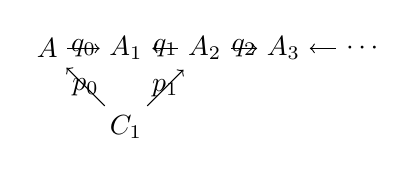
\begin{tikzpicture}
	\node (1) {$A$};
	\node (2) [right of=1] {$A_1$};
	\node (3) [right of=2] {$A_2$};
	\node (4) [right of=3] {$A_3$};
	\node (5) [right of=4] {$\cdots$};
	\node (6) [below of=2] {$C_1$};
	
	\draw [-to] (1) to node {$q_0$} (2);
	\draw [to-] (2) to node {$q_1$} (3);
	\draw [-to] (3) to node {$q_2$} (4);
	\draw [to-] (4) to node {} (5);
	\draw [-to] (6) to node {$p_0$} (1);
	\draw [-to] (6) to node [swap]{$p_1$} (3);	
\end{tikzpicture}
\end{center}
which by composing $p_2$ and $q_2$ reduces the length $r$ zig-zag to a length $r-1$ zig-zag. Hence we can do this for all the cospans in the zig-zag, and the end result will be a simple nice span. 

So, lets assume we have a cospan $A_{i-1}\overset{q_{i-1}}\longrightarrow A_i\overset{q_i}\longleftarrow A_{i+1}$. We could take its pullback, but we have no justification for saying that the maps in the pullback are again quasi-isomorphisms. Since $DGA_k$ is right proper we know that pullback of a weak equivalence along a fibration is again a weak equivalence. By \textbf{MC4} we know that the quasi-isomorphisms $q_{i-1}$ and $q_i$ can be factorized as $q_{i-1} = i \circ q$ and $q_i = j\circ p$, where $q, p$ are cofibrations and $i, j$ are acyclic fibrations. By the two-out-of-three property of weak equivalences, we also know that $q, p$ are acyclic cofibrations. This means we have the following diagram
\begin{center}
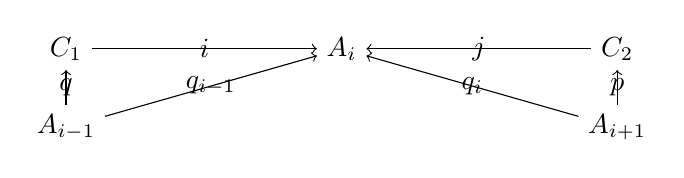
\begin{tikzpicture}
	\node (1) {$C_1$};
	\node (2) [node distance=3.5cm, right of=1] {$A_i$};
	\node (3) [node distance=3.5cm, right of=2] {$C_2$};
	\node (4) [below of=1] {$A_{i-1}$};
	\node (5) [below of=3] {$A_{i+1}$};
	
	\draw [-to] (1) to node {$i$} (2);
	\draw [to-] (2) to node {$j$} (3);
	\draw [-to] (4) to node [swap]{$q_{i-1}$} (2);
	\draw [-to] (5) to node {$q_i$} (2);
	\draw [-to] (4) to node {$q$} (1);
	\draw [-to] (5) to node [swap]{$p$} (3);		
\end{tikzpicture}
\end{center}

Consider now the diagram
\begin{center}
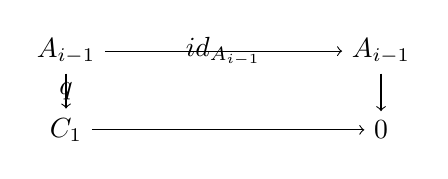
\begin{tikzpicture}
	\node (1) {$A_{i-1}$};
	\node (2) [node distance=4cm, right of=1] {$A_{i-1}$};	
	\node (3) [below of=1] {$C_1$};
	\node (4) [below of=2] {$0$};

	\draw [-to] (1) to node {$id_{A_{i-1}}$} (2);
	\draw [-to] (1) to node [swap]{$q$} (3);
	\draw [-to] (2) to node {} (4);
	\draw [-to] (3) to node {} (4);	
\end{tikzpicture}
\end{center}
As all objects are fibrant we know that $A_{i-1}\longrightarrow 0$ is a fibration. By \textbf{MC3}  there exists a lift, $q'\colon C_1\longrightarrow A$ making the sub-diagrams commute. In particular $q'\circ q = id_{A_{i-1}}$. Since $q$ and $id_{A_{i-1}}$ are both quasi-isomorphisms, $q'$ has to be as well due to the two-out-of-three property. Similarily a quasi-isomorphism $p'$ exists such that $p'\circ p = id_{A_{i+1}}$. 

The next step is to take the pullback of $C_1\overset{i}\rightarrow A_i\overset{j}\leftarrow C_2$, i.e.
\begin{center}
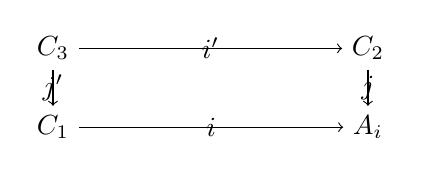
\begin{tikzpicture}
	\node (1) {$C_3$};
	\node (2) [node distance=4cm, right of=1] {$C_2$};	
	\node (3) [below of=1] {$C_1$};
	\node (4) [below of=2] {$A_i$};

	\draw [-to] (1) to node {$i'$} (2);
	\draw [-to] (1) to node [swap]{$j'$} (3);
	\draw [-to] (2) to node {$j$} (4);
	\draw [-to] (3) to node [swap]{$i$} (4);	
\end{tikzpicture}
\end{center}
As $i$ and $j$ are both acyclic fibrations, the maps $i'$ and $j'$ will be as well. This is because being a fibration is stable under pullback, and being a quasi-isomorphism is stable when we are pulling back along a fibration, which both maps are. Now we have a diagram

\begin{center}
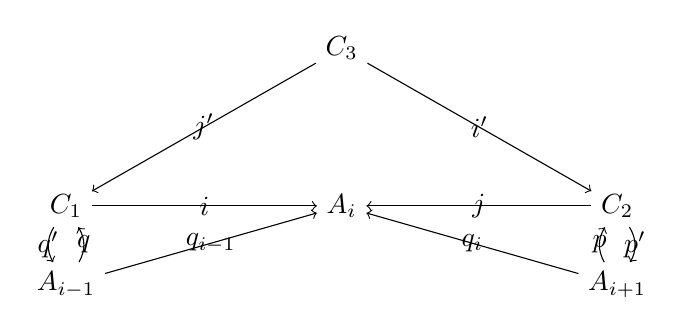
\begin{tikzpicture}
	\node (1) {$C_1$};
	\node (2) [node distance=3.5cm, right of=1] {$A_i$};
	\node (3) [node distance=3.5cm, right of=2] {$C_2$};
	\node (4) [below of=1] {$A_{i-1}$};
	\node (5) [below of=3] {$A_{i+1}$};
	\node (6) [node distance=2cm, above of=2] {$C_3$};
	
	\draw [-to] (6) to node [swap]{$j'$} (1);
	\draw [-to] (6) to node {$i'$} (3);
	\draw [-to] (1) to node {$i$} (2);
	\draw [to-] (2) to node {$j$} (3);
	\draw [-to] (4) to node [swap]{$q_{i-1}$} (2);
	\draw [-to] (5) to node {$q_i$} (2);
	\draw [-to, bend right] (4) to node [swap]{$q$} (1);
	\draw [-to, bend left] (5) to node {$p$} (3);	
	\draw [to-, bend left] (4) to node {$q'$} (1);
	\draw [to-, bend right] (5) to node [swap]{$p'$} (3);				
\end{tikzpicture}
\end{center}

And the compositions $q'\circ i'$ and $p'\circ j'$ are both quasi-isomorphisms, as all four individually are. Hence we have a span $A_{i-1}\longleftarrow C_3 \longrightarrow A_{i+1}$, which by the argument above means we can reduce any zig-zag of quasi-isomorphisms $A\leftarrow \cdots \rightarrow B$ to a single span $A\leftarrow C\rightarrow B$. 
\end{proof}





We don't actually use the specific model structure on $DGA_k$ in this proof, so this holds in for general right proper model categories where all objects are fibrant. 

Notice that this also implies that $DGA_k$ satisfies the right Ore condition, i.e. that given a cospan $A\overset{a}\rightarrow C \overset{q}\leftarrow B$, where $q$ is a quasi-isomorphism, then there exists a span $A\overset{q'}\leftarrow C' \rightarrow B$ where $q'$ is a quasi-isomorphism. This follows from the proof above as we can factorize $a$ into $f\circ c$, where $c$ is an acyclic cofibration and $f$ a fibration. We take the pullback of $D\rightarrow C\leftarrow B$ to get the diagram
\begin{center}
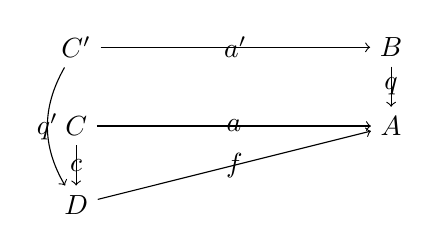
\begin{tikzpicture}
	\node (1) {$C'$};
	\node (2) [node distance=4cm, right of=1] {$B$};	
	\node (3) [below of=1] {$C$};
	\node (4) [below of=2] {$A$};
	\node (5) [below of=3] {$D$};

	\draw [-to] (1) to node {$a'$} (2);
	\draw [-to, bend right] (1) to node [swap]{$q'$} (5);
	\draw [-to] (2) to node {$q$} (4);
	\draw [-to] (3) to node [swap]{$a$} (4);
	\draw [-to] (3) to node {$c$} (5);
	\draw [-to] (5) to node [swap]{$f$} (4);
\end{tikzpicture}
\end{center}
where now $q'$ is a quasi-isomorphism as it is a pullback of one along the fibration $f$. As in the proof above, because $A$ is fibrant we get a left inverse to the acyclic cofibration $c$, which is again a quasi-isomorphism. This is the lift we get from the following diagram
\begin{center}
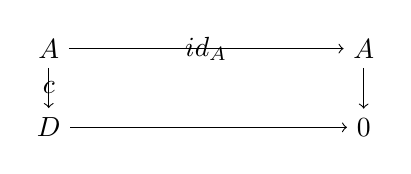
\begin{tikzpicture}
	\node (1) {$A$};
	\node (2) [node distance=4cm, right of=1] {$A$};	
	\node (3) [below of=1] {$D$};
	\node (4) [below of=2] {$0$};

	\draw [-to] (1) to node {$id_A$} (2);
	\draw [-to] (1) to node [swap]{$c$} (3);
	\draw [-to] (2) to node {} (4);
	\draw [-to] (3) to node {} (4);	
\end{tikzpicture}
\end{center}
Denote this lift by $c'$. We now have the final diagram
\begin{center}
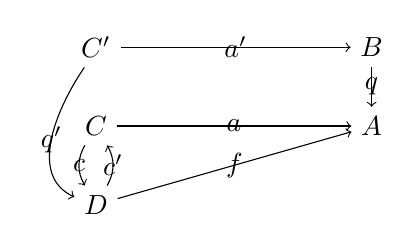
\begin{tikzpicture}
	\node (1) {$C'$};
	\node (2) [node distance=3.5cm, right of=1] {$B$};	
	\node (3) [below of=1] {$C$};
	\node (4) [below of=2] {$A$};
	\node (5) [below of=3] {$D$};

	\draw [-to] (1) to node {$a'$} (2);
	\draw [-to, bend right, in=250] (1) to node [swap]{$q'$} (5);
	\draw [-to] (2) to node {$q$} (4);
	\draw [-to] (3) to node [swap]{$a$} (4);
	\draw [-to, bend right] (3) to node [swap]{$c$} (5);
	\draw [to-, bend left] (3) to node {$c'$} (5);	
	\draw [-to] (5) to node [swap]{$f$} (4);
\end{tikzpicture}
\end{center}
where we by the composition $c'\circ q'$, which is a quasi-isomorphism, we get our wanted span $A\overset{c'\circ q'}\leftarrow C'\rightarrow B$. 

This Ore condition allows the homotopy category $HoDGA_k$ to be described even more explicitly using spans as the morphisms. This means that a morphism $A\longrightarrow B$ is given by a span
\begin{center}
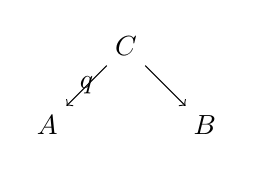
\begin{tikzpicture}
	\node (1) {$A$};
	\node (2) [right of=1] { };	
	\node (3) [right of=2] {$B$};	
	\node (4) [node distance=1cm, above of=2] {$C$};

	\draw [-to] (4) to node [swap]{$q$} (1);
	\draw [-to] (4) to node {} (3);
\end{tikzpicture}
\end{center}
where $q$ is a quasi-isomorphism. Composition of morphisms $A\longrightarrow B$ and $B\longrightarrow C$ is then given as
\begin{center}
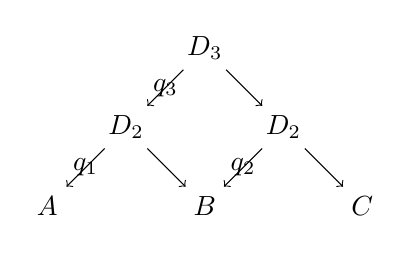
\begin{tikzpicture}
	\node (1) {$A$};
	\node (2) [right of=1] {};	
	\node (3) [right of=2] {$B$};	
	\node (4) [node distance=1cm, above of=2] {$D_2$};
	\node (5) [right of=3] {};
	\node (6) [right of=5] {$C$};
	\node (7) [node distance=1cm, above of=5] {$D_2$};
	\node (8) [right of=4] {};
	\node (9) [node distance=1cm, above of=8] {$D_3$};

	\draw [-to] (4) to node [swap]{$q_1$} (1);
	\draw [-to] (4) to node {} (3);
	\draw [-to] (7) to node [swap]{$q_2$} (3);
	\draw [-to] (7) to node {} (6);	
	\draw [-to] (9) to node [swap]{$q_3$} (4);
	\draw [-to] (9) to node {} (7);		
\end{tikzpicture}
\end{center}
where $q_3$ exists due to the Ore condition. As $q_3\circ q_1$ is again a quasi-isomorphism, we have a new span
\begin{center}
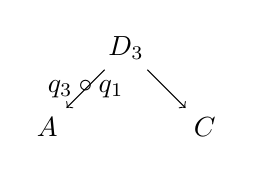
\begin{tikzpicture}
	\node (1) {$A$};
	\node (2) [right of=1] { };	
	\node (3) [right of=2] {$C$};	
	\node (4) [node distance=1cm, above of=2] {$D_3$};

	\draw [-to] (4) to node [swap]{$q_3\circ q_1$} (1);
	\draw [-to] (4) to node {} (3);
\end{tikzpicture}
\end{center}



% \begin{definition}{Homotopy}
% Let $f, g:A\longrightarrow B$ be two DG morphisms. A homotopy $h:f\rightarrow g$ is a map $h:A\longrightarrow B$ such that 
% \begin{itemize}
%     \item $g-f = d_B h + h d_A$
%     \item $h m_A = m_B(f\otimes h + h\otimes g)$
% \end{itemize}
% \end{definition}
% This is definition 4.3. in Proute french thesis

\newpage
\chapter{Massey products}

\tikz[remember picture,overlay]\node[opacity=1,inner sep=0pt] at (current page.center)%
{
\includegraphics[%
clip,
width=1.05\paperwidth,
height=1.05\paperheight
]{chaptertitles/ch2.pdf}};

\clearpage





\section{Motivation}

In the introduction (\ref{sec:introduction}) we said that in some situations, there is some information in the DG-algebra, not accessible to the cohomology algebra of that DG-algebra. On example of such information is given by the Massey products---which will be the focus of this chapter. 

These operations were first introduced to algebraic topology by William S. Massey in \cite{massey}, and have since been used to solve some really interesting problems. One of the reasons Massey products are interesting in topology is due to their ability to distinguish seemingly similar spaces, where other methods fail. The three main invariants we use in algebraic topology to distinguish spaces are homology, cohomology and homotopy. Why do we need all three? It is because none of them are perfect. There are spaces that have the same homology, but are not homeomorphic. Same goes for cohomology and homotopy. We can use these three together to an even greater effect. What we mean is that when two spaces have the same homology and are not homeomorphic, they usually have different homotopy. But, as mentioned in the introduction, the homotopy groups can be extremely difficult to calculate. 

So, what do we do if the spaces have the same homology and the same homotopy? Or that the spaces have the same homology, and the homotopy is really difficult to calculate? Then the next invariant usually is the cohomology ring. The product structure on cohomology allows us a much greater insight into the relationships between parts of the spaces. Usually when we have same homology and same homotopy, we can differentiate them by having different cohomology rings. 

The next question is then, what do we do when all this fails? How can we know spaces aren't homeomorphic even though they have the same cohomology ring? There are many solutions to this answer---and many invariants one could still try---but, Massey products is one of the most developed ones. These operations then tell us when a DG-algebra contains more information than its cohomology algebra, just as we should expect from the introduction. 

In this thesis we have removed the need to work with topologicals spaces, and work only in the algebraic world, so we define the Massey products purely using DG-algebras.  

The main result in this chapter is that for a formal DG-algebra, all Massey products must in some sense be trivial. 

\textbf{Theorem B. } \textit{Let $A$ be a formal DG-algebra. Then $A$ admits no non-vanishing Massey products.}

%The simplest version, the triple Massey product, can famously be used to differentiate three completely separated circles, to the Borromean link. In the case of the normal product structure on the cohomology ring induced by the cup product, we get that the product of two cycles representing two of the rings is a multiple of their linking number, and hence for the Borromean link, the product not internal to any of the three circles is trivial. The product structure in cohomology on the three completely separated links is also trivial in the same way, so the cohomology ring of the Borromean link and the three separated circles is the same. Hence, we need some sort of higher multiplication to check weather objects have some sort of higher linking. 

%This is where the Massey products come in. It turns out that the Borromean link has a non-trivial Massey product, while the three unlinked circles does not. We could try to use just repeated multiplication, i.e. $u\cdot v \cdot w$ to determine higher linking. But, this product is zero for two different reasons as both $u\cdot v = 0$ and $v\cdot w=0$. So we need something else to describe how a kind of triple product can be non-trivial even though the product of all its components are. 

\section{The inaccessible information}

Massey products are often referred to as higher order cohomology operations. We will explain a bit later what this means, but intuitively, it means that they are natural higher arity maps on the cohomology algebra of a DG-algebra. 

\begin{definition}[The triple Massey product]
\label{def:triple_massey}
\index{The triple Massey product}
Let $(A,d)$ be a DG-algebra. Let $x_1, x_2, x_3 \in H(A)$ be three cohomology classes such that $x_1 x_2 = 0 = x_2 x_3$, and let $a_1, a_2, a_3$ be cycles that represent these classes. Since their product is zero in cohomology, there exists classes $b_1$ and $b_2$, such that $d(b_1)=(-1)^{|a_1|}a_1a_2$ and $d(b_2)=(-1)^{|a_2|}a_2a_3$. The cochain 
\begin{equation*}
    x = (-1)^{|a_1|}a_1 b_2 + (-1)^{|b_1|}b_1 a_3
\end{equation*}
is then a cocycle and defines an element in $H^{|x_1|+|x_2|+|x_3|+1}(A)$.  

Since the choices of $b_1$ and $b_2$ are not unique, we define the triple Massey product of $x_1, x_2, x_3$, denoted $\langle x_1, x_2, x_3 \rangle$, to be the set of all such $x$ we can make with different choices for $b_1$ and $b_2$. The elements of the Massey product lie in degree $|x_1|+|x_2|+|x_3|+1$, where the $+1$ comes from the fact that $b_1$ and $b_2$ lie in degree one less than the products $a_1 a_2$ and $a_2 a_3$ respectively. 
\end{definition} 

\begin{remark}
Note that we showed earlier, in \cref{ex:cohomology}, that the product on a DG-algebra induces a well defined product on its cohomology algebra, which we have used in the above definition of the triple Massey product.  
\end{remark}

Notice also that the different elements in the triple Massey product all determine the same element in $H(A)/(x_1H(A)+H(A)x_3)$, hence we could define the triple Massey product to be a morphism from a subset of $H(A)\times H(A)\times H(A)$ to $H(A)/(x_1H(A)+H(A)x_3)$. This subset would then have to be the set of elements $x_1, x_2, x_3$ such that $x_1x_2 = 0 = x_2x_3$. Since this method does not generalize well to the higher Massey products we want to define, we do not use this definition. 

As said, generalizing this construction is a bit tedious explicitly, so we instead find a suitable workaround by using so-called defining systems. 

\begin{definition}[Defining system]
\label{def:defining_system}
\index{Defining system}
Let $\bar{x} = (-1)^{|x|}x$. A defining system for a set of cohomology classes $x_1, \ldots, x_n$ in $ H(A)$ is a collection $\{ a_{i,j}\}$ of cochains in $A$ such that
\begin{itemize}
    \item $[a_{i-1, i}] = x_i$
    \item $d(a_{i, j}) = \displaystyle\sum_{i<k<j}\overline{a_{i, k}}a_{k, j}$
\end{itemize}
for all pairs $(i,j)\neq (0,n)$ where $i\leq j$.
\end{definition}

These defining systems allow us to quite easily define Massey products of any order. 

\begin{definition}[Massey $n$-product]
\label{def:massey_product}
\index{Massey product}
The Massey $n$-product of $n$ cohomology classes $x_1, \ldots, x_n$, denoted $\langle x_1, \ldots, x_n\rangle$, is defined to be the set of all $[a_{0,n}]$, where
\begin{equation*}
    a_{0,n} = \sum_{0<k<n}\overline{a_{0, k}}a_{k, n}
\end{equation*}
such that $\{ a_{i,j} \}$ is a defining system.
\end{definition}

Let's write this out in a bit more detail for some small $n$ and see what we get. 

$\mathbf{n=2}:$ Assume we have two cohomology classes $x_1$ and $x_2$ and a defining system $\{a_{i,j} \}$. The defining system will just be $\{ a_{0,1}, a_{1,2}\}$ such that $[a_{0,1}]=x_1$ and  $[a_{1,2}] = x_2$. The element in the Massey product---given by the defining system---is then $[a_{0,2}]$, where $a_{0, 2} = \overline{a_{0, 1}}a_{1, 2}$. This is just the cohomology class of the product in the DG-algebra up to a sign. Hence Massey $2$-products are already familiar. 


$\mathbf{n=3}:$ Let now $x_1, x_2, x_3$ be three cohomology classes and $\{a_{i,j}\}$ a defining system for them. The system will consist of $a_{0,1}, a_{1,2}, a_{2,3}, a_{0,2}$ and $a_{1,3}$ such that 
\begin{itemize}
    \item $[a_{0,1}] = x_1$
    \item $[a_{1,2}] = x_2$
    \item $[a_{2,3}] = x_3$
    \item $d(a_{0,2}) = \overline{a_{0,1}} a_{1,2}$
    \item $d(a_{1,3}) = \overline{a_{1,2}} a_{2,3}$.
\end{itemize}
This means that the element in the Massey product $\langle x_1, x_2, x_3 \rangle$ defined by the defining system above is given by $[a_{0,3}]$, where
\begin{equation*}
    a_{0,3} = \overline{a_{0, 1}}a_{1, 3} + \overline{a_{0, 2}}a_{2, 3}.
\end{equation*}
This we see is exactly the same as the triple Massey product we defined in the beginning, before introducing the defining systems. Hence this way to generalize the definition is actually a generalization. 

$\mathbf{n=4}:$ Let $x_1, x_2, x_3, x_4$ be cohomology classes and $\{ a_{i,j} \}$ be a defining system for them. It consists of nine elements $a_{0,1}, a_{1,2}, a_{2,3}, a_{3,4}, a_{0,2}, a_{1,3}, a_{2,4}, a_{0,3}, a_{1,4}$ such that 
\begin{itemize}
    \item $[a_{0,1}] = x_1$
    \item $[a_{1,2}] = x_2$
    \item $[a_{2,3}] = x_3$
    \item $[a_{3,4}] = x_4$
    \item $d(a_{0,2}) = \overline{a_{0,1}} a_{1,2}$
    \item $d(a_{1,3}) = \overline{a_{1,2}} a_{2,3}$
    \item $d(a_{2,4}) = \overline{a_{2,3}} a_{3,4}$
    \item $d(a_{0,3}) = \overline{a_{0,1}} a_{1,3}+\overline{a_{0,2}}a_{2,3}$
    \item $d(a_{1,4}) = \overline{a_{1,2}} a_{2,4}+\overline{a_{1,3}}a_{3,4}$.
\end{itemize}
This makes the element in $\langle x_1, x_2, x_3, x_4\rangle$ defined by the defining system $\{a_{i,j}\}$ equal to $[a_{0,4}]$, where
\begin{equation*}
    a_{0,4} = \overline{a_{0,1}}a_{1,4} + \overline{a_{0,2}}a_{2,4} + \overline{a_{0,3}}a_{3,4}.
\end{equation*}

For the rest of this thesis, when we talk about Massey products, we mean Massey $n$-products for $n\geq 3$, for precisely this reason that Massey $2$-products are just given by multiplication. When we say ``all Massey products'' we will mean all Massey $n$-products, for all $n\geq 3$. 

We wanted these Massey products to serve as information not accessible to the cohomology algebra, and we will soon define what we mean by this and show that this is in fact the case. In order to do this we will need the following important definition. 

\begin{definition}[Vanishing Massey product]
\label{def:vanishing_massey}
\index{Vanishing Massey product}
Let $\langle x_1, \cdots, x_n\rangle$ de a defined Massey product in a DG-algebra $A$. We say it vanishes if it contains zero as an element, i.e. $0\in \langle x_1, \ldots, x_n\rangle$. 
\end{definition}

Since the Massey $n$-product is a set, we cant in general hope for it being just the zero class, so this definition of a vanishing Massey product is the closest thing we can have to a ``trivial'' Massey product. 

\begin{definition}[Uniquely defined Massey product]
\label{def:uniquely_defined_massey}
\index{Uniquely defined Massey product}
We say that a Massey $n$-product, $\langle x_1, \ldots, x_n\rangle$, is uniquely defined if it contains only a single class, i.e. $\langle x_1, \ldots, x_n\rangle=\{x\}$. 
\end{definition}

In the case of an uniquely defined Massey product, we can say it is trivial if this element is the zero class. We will however still use the word ``vanishing'', as it is more general, and more suitable for our purposes. 

Let's see some examples of DG-algebras with some Massey products in order to get a feeling for how they work. 

\begin{example}
Let $A$ be the DG-algebra $k[x_1,x_2,x_3,a,b]$, with product given by normal multiplication, and where $x_1, x_2, x_3, a, b$ all have degree $1$. Let further $d(x_1)=d(x_2)=d(x_3)=0$, $d(a)=x_1\cdot x_2$ and $d(y)=x_2\cdot x_3$. 

Since $x_1\cdot x_2$ and $x_2\cdot x_3$ are coboundaries, they are representatives for the zero class in cohomology. We also have predefined, preferred cochains that hit them under $d$, namely $a$ and $b$. 

This means that by construction we have a non-trivial element of the Massey 3-product $\langle x_1, x_2, x_3\rangle$, given by $[\overline{a}\cdot x_1 + \overline{x_3}\cdot b]$. 
\end{example}

\begin{example}
\label{ex:borromean_rings}
When talking about Massey products it is customary to mention the application to proving that \emph{the Borromean rings}\index{The Borromean rings} are not homeomorphic to the triple unlink. 

\begin{center}
\def\svgwidth{0.8\textwidth}
\input{images/borromean+unlink.pdf_tex}
\end{center}

These spaces both consist of three copies of $S^1$, embedded in $\R^3$. The triple unlink is three completely separated components, but the Borromean link can not be separated into its three components. The fact that this can't happen is difficult to prove mathematically, and it was not properly understood how it could be proven until Massey products came to the rescue. 

We won't prove this fact here, as it requires more in depth look into the topological side of these operations, but we can sketch the intuition. These two spaces both have the same cohomology ring, due to the cup product in the cohomology ring of the complement of the spaces measures the linking number of the rings. Since all of the three copies of $S^1$ in the Borromean link---and the triple unlink---are pairwise unlinked we have that the cup product vanishes on cochains that represent these circles. This means that the cohomology ring is the same, and that some Massey $3$-product is defined for both spaces. 

For the triple unlink, the Massey 3-product will be trivial, but for the Borrmoean link there will be some non-trivial elements. For a proper proof see \cite{linking}. \footnote{Note that this paper was originally presented by Massey in 1968 at a conference at the University of Illinois. The article referenced above has later been written in \TeX{} by Elaine Jackson.}
\end{example}

\begin{example}
There are also other types of non-trivial links, for example the following one, consisting of four copies of $S^1$:

\begin{center}
\def\svgwidth{0.7\textwidth}
\input{images/4-link.pdf_tex}
\end{center}

Here we have that any subset of three circles are unlinked, so the Massey 3-product is not enough to show that the whole link is not the unlink. We can however do this by using Massey 4-products, as shown in \cite{four-link}. 
\end{example}



\section{Relation to formality}

In the introduction we intuitively defined formal DG-algebras to be the ones where their cohomology algebras contain all the ``relevant information''.  We have now introduced Massey products as a type of information that should contradict this, i.e. information that is inaccessible to the cohomology algebra. Intuitively, being formal should then mean that no non-vanishing Massey products can exist. We will see that this is in fact the case.

%We now study the relationship between formal DG algebras and their Massey products. Being formal means that we can get back our DG algebra from its cohomology algebra, and that means that there is no important information lost when passing to cohomology. Intuitively at least, Massey products should measure higher information in the DG algebra, that we cant see directly from cohomology. 

%From the Borromean link example, cohomology only sees the pairwise linking of the circles, which there is none, but fails to see the higher linking. So intuitively we expect having vanishing Massey products means there is no such higher information, and hence the cohomology algebra has enough to reconstruct the DG algebra. This is formalized in the question; is a DG algebra with vanishing Massey products formal? This turns out to almost be true, but not in this exact formulation. There are examples of DG algebras with vanishing Massey products that are not formal. But, if we can have vanishing Massey products in a ``nice'' way, i.e. that they all vanish for the same reason, then we will have a formal DG algebra. The converse statement though, is true. We cant have higher information, i.e. Massey products, if we know it is formal. 

Recall that (by \cref{thm:span}) a DG-algebra $A$ is called formal\index{Formal DG-algebra} there is a span of quasi-isomorphism
\begin{equation*}
	H(A)\longleftarrow C \longrightarrow A
\end{equation*}
for some DG-algebra $C$. 

\begin{theorem}
\label{thm:formal_no_massey}
Let $(A, d_A)$ be a formal DG-algebra. Then all Massey $n$-products vanish, i.e. given cohomology classes $x_1, \ldots, x_n$ such that their Massey $n$-products is defined, then we have $0\in \langle x_1, \ldots, x_n\rangle$. 
\end{theorem}

This result is remarked as being true---for positively graded minimal DG-algebras---in \cite[Theorem 4.1.]{DGMS}. It is proven using the same techniques and same assumptions in \cite[Theorem 1.6.5]{exact-massey}. As we do not use the above assumptions, we weren't certain that the referenced proof could be fitted to our more general case. Thus we use a more lengthy, but simpler approach, which also allows us to discuss elements from the introduction in a mathematically rigorous way. Our strategy is to prove it using the naturality of Massey products in combination with a DG-algebra with $d=0$ having vanishing Massey products. So lets prove these first.

\begin{lemma}
\label{lm:naturality_of_massey}
Let $f\colon A\longrightarrow B$ be a morphism of DG-algebras, $f^*$ be its induced morphism in cohomology and $\langle x_1, \ldots, x_n\rangle $ a defined Massey $n$-product in $A$. Then we have $f^*( \langle x_1, \ldots, x_n\rangle) \subseteq \langle f^*(x_1), \ldots, f^*(x_n)\rangle$. 
\end{lemma}
\begin{proof}
Let $x\in \langle x_1, \ldots, x_n\rangle$. Then there exists a defining system $\{a_{i,j\}}\subseteq A$ for $x$, such that $[a_{0,n}] = x$, where  
\begin{equation*}
    a_{0,n} = \sum_{0<k<n}\overline{a_{0,k}}a_{k,n}.
\end{equation*}
Notice that we have 
\begin{equation*}
    f^*(x) = [f(a_{0,n})] = [f(\sum_{0<k<n}\overline{a_{0,k}}a_{k,n})] = [\sum_{0<k<n}\overline{f(a_{0,k})}f(a_{k,n})]
\end{equation*}
hence proving that $\{ f(a_{i,j})\}$ is a defining system for $f^*(x)$ will prove the lemma. 

We have that $[f(a_{i-1,i})] = f^*[a_{i-1,i}] = f^*(x_i)$, which proves the first criterion. The last part follows from the fact that a morphism of DG-algebras commutes with the differentials. Explicitly we have
\begin{align*}
    d(f(a_{i,j}))
    &= f(d(a_{i,j})) \\
    &= \sum_{i<k<j}f(\overline{a_{i,k}})f(a_{k,j}) \\
    &= \sum_{i<k<j}\overline{f(a_{i,k})}f(a_{k,j})
\end{align*}
where the second equality uses the fact that $f(\overline{a_{i,j}}) = \overline{f(a_{i,j})}$. 
\end{proof}

This is what justifies calling them cohomology operations. This name comes  from algebraic topology---where a cohomology operation is a map between cohomology groups that are natural with respect to continuous maps between topological spaces. This means that they form natural transformations between cohomology functors. For our algebraic setting we have that maps between topological spaces induce maps between their algebraic model, hence we still use the term cohomology operation to describe natural transformations between cohomology functors in this algebraic setting as well. Notice that strictly speaking, the Massey products are not cohomology operations, as they consist of a set, rather than a single element. So calling them cohomology operations is in a broad sense. If however the Massey products consists of a single element, i.e. they are uniquely defined, then they are actual cohomology operations. 

The Massey 3-product is called a cohomology operation of order 2, because it requires a relation on cohomology operations of order 1 to be true. For the Massey 3-product, this relation is the vanishing of the induced products, $x_1 x_2 = 0 = x_2 x_3$. This induced product is a cohomology operation as it is natural with respect to maps between DG-algebras. The Massey $n$-product is then a cohomology operation of order $n-1$, as it places a restriction on some cohomology operation of order $n-2$ to be defined.   


\begin{theorem}
\label{thm:quasi_preserves_massey}
If $q\colon A\longrightarrow B$ is a quasi-isomorphism of DG-algebras and $x_1, \ldots, x_n$ cohomology classes such that $\langle x_1, \ldots, x_n\rangle$ is defined, then 
\begin{equation*}
    q^*(\langle x_1, \ldots, x_n\rangle) = \langle q^*(x_1),\ldots, q^*(x_n)\rangle .
\end{equation*}
\end{theorem}

This proof is inspired by the much more general proof of the more general statement in \cite[Theorem 1.5]{naturality}. There the same statement is proven to hold for more general types of Massey products, called matric Massey products, as well as for more general types of quasi-isomorphisms, which we will encounter later in the thesis (\cref{ssec:A_infinity-morphisms}). 

\begin{proof}
From the naturality of Massey products we know that 
\begin{equation*}
    q^*(\langle x_1, \ldots, x_n\rangle) \subseteq \langle q^*(x_1),\ldots, q^*(x_n)\rangle
\end{equation*}
so it remains to show the reverse containment. 

Let $y\in \langle q^*(x_1), \ldots, q^*(x_n)\rangle$ and $\{b_{i,j}\}$ be a defining system for it. Recall that this means in particular that we have some $b_{0,n}$ such that $[b_{0,n}] = y$. We will construct a defining system $\{a_{i,j}\}$ for some $x\in \langle x_1, \ldots, x_n\rangle $ such that $ q(a_{0,n})$ is cohomologous to $b_{0,n}$. We construct this defining system $\{a_{i,j}\}$ using induction on $j-i$. 

Let $a_{i-1, i}$ be any representative of $x_i$. This means that both $q(a_{i-1, i})$ and $b_{i-1, i}$ are representatives for $q^*(x_i)$ , which gives us that their difference in cohomology is zero, i.e. 
\begin{equation*}
    [q(a_{i-1, i})]-[b_{i-1, i}] = 0.
\end{equation*}
This means that we have some $c_{i-1, i} \in B$ such that
\begin{equation*}
    d_B(c_{i-1, i}) = q(a_{i-1, i}) - b_{i-1, i}.
\end{equation*}

Now, assume that for any $p$ with $1<p\leq n-2$ we have constructed $a_{k,l}$ and $c_{k,l}$ for any $k,l$ with $1< l-k<p$, such that 
\begin{align}
    d(a_{k,l}) &= \sum_{m=k+1}^{l-1}\overline{a_{km}}a_{ml} 
    \\
    d(c_{k,l}) &= q(a_{k,l}) - b_{k,l} \sum_{m=k+1}^{l-1}\overline{c_{k,m}}q(a_{m,l}) + b_{k,m}c_{m,l}.
\end{align}
Notice that these hold for our already constructed $a_{i-1, i}$ and $c_{i-1, i}$. Notice also that as $q$ and $d$ commute, we have 
\begin{equation*}
    d(q(a_{k,l}) = \sum_{m=k+1}^{l-1}\overline{q(a_{km})}q(a_{ml}) .
\end{equation*}

Let $p = j-i$. Then 
\begin{align*}
    d\left(\sum_{k=i+1}^{j-1}\overline{c_{ik}}q(a_{kj})+b_{ik}c_{kj}\right)
    &= \sum_{k=i+1}^{j-1}d(\overline{c_{ik}}q(a_{kj}))+d(b_{ik}c_{kj}) \\
    &= \sum_{k=i+1}^{j-1} d(\overline{c_{i,k}})q(a_{k,j}) + (-1)^{|\overline{c_{ik}}|}\overline{c_{i,k}}d(q(a_{k,j})) \\
    &\hspace{13mm}+ 
    d(b_{i,k})c_{k,j} + (-1)^{|b_{i,k}|}b_{i,k}d(c_{k,j})
\end{align*}
which by equation (2.1) and (2.2) is equal to  
\begin{align*}
\sum_{k=i+1}^{j-1} \overline{q(a_{i,k}}q(a_{k,j}) + \overline{b_{i,k}}q(a_{k,j})
    &+ 
    \sum_{m = i+1}^{k-1}\overline{c_{i,m}q(a_{m,k})}q(a_{k,j}) + \overline{b_{i,m}c_{m,k}}q(a_{k,j}) \\
    &+ 
    (-1)^{|\overline{c_{i,k}}|}\overline{c_{i,k}}\left(\sum_{m=k+1}^{j-1}\overline{q(a_{k,m})})q(a_{m,j}\right) \\
    &+ 
    \sum_{m=i+1}^{j-1}\overline{b_{i,m}}b_{m,k}c_{k,j} + (-1)^{|b_{i,k}|}(b_{i,k}q(a_{k,j}) - b_{i,k}b_{k,j}) \\
    &+ 
    (-1)^{|b_{i,k}|}\left(\sum_{m=k+1}^{j-1}b_{i,k}\overline{c_{k,m}}q(a_{m,j})+b_{i,k}b_{k,m}c_{m,j}\right).
\end{align*}
This gives us---by canceling the terms with opposite signs---finally
\begin{equation*}
d\left(\sum_{k=i+1}^{j-1}\overline{c_{ik}}q(a_{kj})+b_{ik}c_{kj}\right) = \sum_{k=i+1}^{j-1}\overline{b_{i,k}}b_{k,j} + \sum_{k=i+1}^{j-1}\overline{q(a_{a_{i,k}})}q(a_{k,j}).
\end{equation*}
Since $\{b_{i,j}\}$ is a defining system, we know that $\sum_{k=i+1}^{j-1}\overline{b_{i,k}}b_{k,j}$ is a coboundary, which by the above calculation means that also $\sum_{k=i+1}^{j-1}\overline{q(a_{i,k})}q(a_{k,j})$ is a coboundary. Since $q$ and $d$ commute, we also get that $\sum_{k=i+1}^{j-1}\overline{a_{i,k}}a_{k,j}$ is a coboundary. Hence we can choose some $a_{i,j}'$ such that
\begin{equation*}
    d(a_{i,j}') = \sum_{k=i+1}^{j-1}\overline{a_{i,k}}a_{k,j}.    
\end{equation*}
We use this to define an element 
\begin{equation*}
    e_{i,j} = q(a_{i,j}') - b_{i,j} + \sum_{k=i+1}^{j-1}\overline{c_{i,k}}q(a_{k,j})+b_{i,k}c_{k,j}
\end{equation*}
which is a cocycle. We can then choose another cocycle $d_{i,j}$ such that $q(d_{i,j})$ is cohomologous to $e_{i,j}$. This means that their difference is zero in cohomology, i.e. 
\begin{equation*}
    [q(d_{i,j})]-[e_{i,j}] = 0
\end{equation*}
Hence there exists some $c_{i,j}$ such that 
\begin{equation*}
    d(c_{i,j}) = q(d_{i,j}) - e_{i,j}.
\end{equation*}
If we let $a_{i,j} = a_{i,j}-d_{i,j}$ then we have 
\begin{align*}
    d(a_{i,j}) &= \sum_{k=i+1}^{j-1}\overline{a_{ik}}a_{kj} 
    \\
    d(c_{i,j}) &= q(a_{i,k}) - b_{i,k} \sum_{k=i+1}^{j-1}\overline{c_{i,k}}q(a_{k,j}) + b_{i,k}c_{k,j}.
\end{align*}
By induction we now have the elements $a_{i,j}$ and $c_{i,j}$ for all $i,j$ such that $1<i-j<n$. The exact same long calculation as we just did---exchanging $i,j$ by $0,n$---shows that 
\begin{align*}
    d\left(\sum_{k=1}^{n-1}\overline{c_{0k}}q(a_{kn})+b_{0k}c_{kn}\right)
    &=
    \sum_{k=1}^{n-1}\overline{b_{0,k}}b_{k,n} + \sum_{k=1}^{n-1}\overline{q(a_{a_{0,k}})}q(a_{k,n}) \\
    &= b_{0,n} - q(a_{0,n})
\end{align*}
which means that $b_{0,n}$ and $q(a_{o,n})$ are cohomologous, as they differ by a boundary. 

To summarize, we have for any $y$ in $ \langle q^*(x_1), \ldots, q^*(x_n)\rangle$ found a $q^*(x)$ in $q^*(\langle x_1, \ldots, x_n\rangle)$, such that $q^*(x)=y$ in cohomology, hence
\begin{equation*}
    \langle q^*(x_1), \ldots, q^*(x_n)\rangle \subseteq q^*(\langle x_1, \ldots, x_n\rangle)
\end{equation*}

By putting the two containments together we get our wanted set-equivalence 
\begin{equation*}
    \langle q^*(x_1), \ldots, q^*(x_n)\rangle = q^*(\langle x_1, \ldots, x_n\rangle)
\end{equation*}
\end{proof}


\begin{corollary}
\label{cor:quasi_preserves_vanishing}
If $q\colon A\longrightarrow B$ is a quasi-isomorphism, then all Massey products in $A$ vanish if and only if all Massey products vanish in $B$. 
\end{corollary}

This means that having vanishing Massey products is a ``stable property'' through quasi-isomorphisms. The next thing we need for our result, is that a DG-algebra with trivial differential, can't have any non-vanishing Massey products. 

\begin{lemma}
\label{lm:trivial_differential_then_no_massey}
Any DG-algebra $(A, d)$ with $d=0$ has no non-vanishing Massey products.
\end{lemma}

\begin{proof}
Take a Massey n-product $\langle x_1, \ldots, x_n\rangle$ in $A$. Since the differential in $A$ is the zero map we know that its cohomology is equal to it self, hence the cochains that represent $x_i$ can be chosen to be $x_i$ itself. Lets look at the case $n=3$ first for some intuition. 

Since $[x_1][x_2]=0=[x_2][x_3]$ we know that $x_1 x_2 =0$, as the cochains represent themselves. This means that when we chose a cochain $u$ such that $d(u)=x_1 x_2$ we can chose $u=0$, and similarily $v=0$ for a cochain such that $d(v)=x_2 x_3$. Hence $\overline{u}x_1+\overline{x_3}v = 0x_1+\overline{x_3}0=0$, which means that $0$ is an element in the Massey product $\langle x_1, x_2, x_3\rangle$, i.e. it is trivial. 

This is also the idea generally. Since the cohomology classes represent themselves we can always find a defining system consisting mostly of zeroes. What we mean is the following. Let $\langle x_1, \ldots, x_n\rangle$ be defined. Any defining system $\{a_{i,j}\}$ used to define an element in it must have 
\begin{equation*}
    0 = d(a_{i,j}) = \sum_{i<j<k}\overline{a_{i,k}} a_{k,j}
\end{equation*}
for all $(i,j)\neq (0,n)$, as $d=0$. This means that for $i,j$ such that $(i,j)\neq (0,n)$ and $(i,j)\neq (i,i+1)$ we can choose $a_{i,j} = 0$. As $d$ is linear we get
\begin{equation*}
    d(0)=0=\sum_{i<j<k}\overline{a_{i,k}} a_{k,j}.
\end{equation*}
Thus, if we let $a_{i-1, i} = x_i$, then $\{ x_1, x_2,\ldots, x_n, 0, \ldots, 0 \}$ is a defining system for $x_1, \ldots, x_n$. This defining system produces the zero element
\begin{equation*}
    a_{0,n} = \sum_{0<j<n}\overline{a_{0,k}} a_{k,n} = 0
\end{equation*}
because every summand must contain a copy of the zero class. This means that $0\in \langle x_1, \ldots, x_n\rangle$ for any $n$ and any $x_1, \ldots, x_n \subseteq H(A)$, meaning that all Massey products of all orders must be vanishing.
\end{proof}

The above lemma is the precise mathematical formulation of the statement that the cohomology algebra of a DG-algebra does not have ``access to the information'' that the Massey products contain. The cohomology algebra of a DG-algebra is precisely one such DG-algebra with trivial differential, hence there can be no non-vanishing Massey products. This means that the cohomology algebra does not contain all the relevant information, given that there is some non-trivial Massey products in the original DG-algebra. 

Ok, lets put these lemmas together to form the proof of the fact that a formal DG-algebra can have no non-vanishing Massey products. 

\begin{proof}[of theorem 2.8]
Given a formal DG-algebra $A$ there is by \cref{thm:span} a span of quasi-isomorphisms $H(A)\longleftarrow C\longrightarrow A$. By \cref{lm:trivial_differential_then_no_massey} all Massey products in $H(A)$ must contain the zero class, as it is a DG-algebra with trivial differential. By \cref{cor:quasi_preserves_vanishing} we know that $H(A)$ only having vanishing Massey product implies that $A$ only has vanishing Massey products, as they are connected by quasi-isomorphisms. 
\end{proof}

This resolves \textbf{Theorem B.} from the motivation of the chapter. Having now proven that formal DG-algebras admit no non-vanishing Massey products means that having any non-trivial Massey product is a definite obstruction to being a formal DG-algebra, which is exactly what we expected. It is information--inaccessible to the cohomology algebra---hence the DG-algebra can't be sufficiently simple. This also 	gives us a criteria for answering negative to our central question: 

\begin{central}
Given a DG-algebra $A$, when do we know that $A$ is formal?
\end{central}
\textbf{Criteria:} All Massey products needs to be vanishing, if not, $A$ can't be formal. 

Notethat any DG-algebra $G$ with $d=0$ must be formal, as the map $G\longrightarrow H(G)$ sending $g$ to its cohomology class $[g]$ induces an isomorphism in cohomology---namely the identity map. This means that we can include the category of graded algebras into the category $DGA_k$ by letting $d=0$, project down to the homotopy category $hoDGA_k$ and look at its essential image, i.e. all objects in $hoDGA_k$ that are isomorphic to an algebra in the image of the functor
\begin{center}
\begin{tikzcd}
GrAlg_k \arrow[r, "I"] & DGA_k \arrow[r, "\pi"] & hoDGA_k
\end{tikzcd}    
\end{center}
Taking the essential image
\begin{equation*}
    \text{eIm}(\pi\circ I) = \{A\in hoDGA_k \,\vert\, A\cong \pi( I(G)) \text{ for some } G\in GrAlg_k\}
\end{equation*}
should give us precisely the homotopy category of the subcategory of formal DG-algebras. 

This means we have a partial answer to the central question.

\textbf{Partial answer:} When $A$ has a trivial differential. 

It would not be very exciting if these were all the formal DG-algebras, and we know for a fact that they are not, as we earlier saw examples of this. Thus our pursuit of a definite answer continues. 

A natural more general question after this is then: Are the Massey products the \emph{only} obstructions to having formality? Or more mathematically, if all Massey products in a DG-algebra $(A,d)$ vanish, is $A$ formal? If this were the case we would have an answer to our central question:

\textbf{Potential answer:} When $A$ has no non-trivial Massey products.

This sadly turns out to \emph{not} be the case. This should maybe be expected intuitively, as information hidden from the cohomology algebra could in theory be anything. So having the only such information being the Massey products would imply that no ``weird things'' could happen, and in the field of topology, weird things happen more often than not. For some examples of non-formal DG-algebras, with only vanishing Massey products, see \cite[Section 1.5]{non_formal1} and \cite[Example 8.13.]{non_formal2}. 

\subsection*{The path onwards}

We are now facing a cross-road. Our attempted method of checking formality didn't work as well as we wanted, so where do we go? Do we try something new? Some other invariants, or techniques to detect formality? There is some interesting theory developed around formality and Hochschild cohomology. One can calculate certain Hochschild cohomology classes---for example the so-called Kaledin class, developed in \cite{kaledin1} and \cite{kaledin2}---which only vanish when the DG-algebra is formal. 

We will however walk another way, continuing more along the same route. By this we mean that we will try to rectify the theory we have already developed by using generalizations. More specifically, we need access to even more homotopical information. We will take a DG-algebra, and in some sense homotopically deform it, so that we get a weaker, but richer structure---containing even more homotopical information. 






\newpage
\chapter{Transferring algebraic structures}
\label{ch:3}
\tikz[remember picture,overlay]\node[opacity=1,inner sep=0pt] at (current page.center)%
{
\includegraphics[%
clip,
width=1.05\paperwidth,
height=1.05\paperheight
]{chaptertitles/ch3.pdf}};

\clearpage


\section{Transferring algebraic structures}

Imagine we have a system of two topological spaces $f:T\longrightarrow G$. We are often interested in knowing if a certain property on the space $G$ can be transferred through $f$ such that we have the same property on $T$. If $f$ is a nice enough morphism an example could be a topological invariant of $G$, for example its Euler characteristic. Transferring invariants is an important and rich field of study in topology, but in this thesis we are more interested in transferring other things than invariants, more specifically structures. If $G$ has an algebraic structure, for example a group structure, can we then transfer the same or some other similar structure onto $T$ through $f$?

Let's assume for now that $G$ is a group and that $f$ is an isomorphism. This allows us to also make $T$ into a group by transferring the group structure through $f$. We get this by defining the multiplication on $T$ to be $t_1\cdot t_2 = f^{-1}(f(t_1)\cdot f(t_2))$. Let's prove that this is a group structure on $ T$. 

Since $ f$ is an isomorphism, we have a unique element that gets sent to the identity element in $ G$, which we define to be the identity element of $ T$, i.e. $ 1_T = f^{-1}(1_G)$. This is in fact an identity element since
\begin{align*} 
t\cdot 1_T &= f^{-1}(f(t)\cdot f(1_T)) \\ 
&= f^{-1}(f(t)\cdot f(f^{-1}(1_G))) \\ 
&= f^{-1}(f(t)\cdot 1_G) \\ 
&= f^{-1}(f(t)) \\ 
&= t . 
\end{align*}

 
The same holds for $ 1_T\cdot t = t$. We define the inverse of an element to be $ t^{-1} = f^{-1}((f(t)^{-1})$. Which we see is an inverse because
\begin{align*} 
t\cdot t^{-1} 
&= f^{-1}(f(t)\cdot f(t^{-1})) \\ 
&= f^{-1}(f(t)\cdot f(f^{-1}((f(t))^{-1}))) \\ 
&= f^{-1}(f(t)\cdot (f(t))^{-1}) \\ 
&= f^{-1}(1_G) \\ 
&= 1_T, 
\end{align*}

 
where the same also holds for $ t^{-1}\cdot t = 1_T$. The operation is associative because
\begin{align*} 
t_1\cdot (t_2\cdot t_3) 
&= t_1\cdot (f^{-1}(f(t_2)\cdot f(t_3)))\\ 
&= f^{-1}(f(t_1)\cdot f(f^{-1}(f(t_2)\cdot f(t_3)))) \\ 
&= f^{-1}(f(t_1)\cdot (f(t_2)\cdot f(t_3))) \\ 
&= f^{-1}((f(t_1)\cdot f(t_2))\cdot f(t_3)) \\ 
&= f^{-1}(f(f^{-1}(f(t_1)\cdot f(t_2)))\cdot f(t_3)) \\ 
&= (f^{-1}(f(t_1)\cdot f(t_2))\cdot t_3 \\ 
&= (t_1\cdot t_2)\cdot t_3 
\end{align*}
where the equality between the third and the fourth line comes from the associativity of the product in $G$.
 
Hence we have a binary operation on $T$ which is associative, has an identity element and has all inverses, which makes $T$ into a group.

A crucial part in the above proof is that $f$ is an isomorphism, so what happens when this is not the case? In the words of George Orwell, ``All ways of getting from $T$ to itself are equal, but some are more equal than others'', so if we choose a morphism with a weaker type of inverse than an isomorphism, we can develop something interesting. We have already seen such maps with a weaker form of inverse, namely homotopy equivalences. In this situation, what happens to the same kind of transferred structure on $T$? We do the same thing as earlier and define our operation to be given by $m_2(t_1, t_2)=t_1\cdot t_2 = g(f(t_1)\cdot f(t_2))$. Why we also denote it by $ m_2$ will be clearer later. This is a map $ T\times T\longrightarrow T$. One thing we can check is weather this map is still associative. We have
\begin{align*} 
t_1\cdot (t_2 \cdot t_3) 
&= t_1\cdot g(f(t_2)\cdot f(t_3)) \\ 
&= g(f(t_1)\cdot fg(f(t_2)\cdot f(t_3))) 
\end{align*}

and
\begin{align*} 
(t_1\cdot t_2) \cdot t_3 
&= g(f(t_1)\cdot f(t_2)) \cdot t_3\\ 
&= g(fg(f(t_1)\cdot f(t_2))\cdot f(t_3)) 
\end{align*}

which because $ g\circ f \neq id_T$, are not equal in general. Luckily they are homotopic! So instead of actual associativity, we have associativity up to homotopy. Such a homotopy between them is a map $ m_3:I\times T^3\longrightarrow T$, where $ I$ is the unit interval. This means that the interval parameterizes a space of maps $ T^3\longrightarrow T$ in such a way that on the edges of the interval we have the two ways of combining three elements by our operation $ m_2$. Another way to say this is that the composition of $ m_3$ with the boundary map $ \partial$ is given by 

$ m_2(id_T\times m_2) - m_2(m_2 \times id_T) - m_3(\partial \times id_T \times id_T + id_T\times \partial \times id_T + id_T\times id_T\times \partial )$.

We can graphically visualize the parameterization by the following picture:

\begin{center}
\def\svgwidth{0.6\textwidth}
\input{images/K3_brackets.pdf_tex}
\end{center}


Here the two ends are the different brackets we can put between the elements in order to get the two different operations using $ m_2$. The line between them is the homotopy $m_3$.

The line we just constructed, i.e. the space that parametrizes operations $ T^3\longrightarrow T$ is called the third Stasheff associahedra, which we denote by $K3$. A natural question to ask is if we can continue this process, i.e. to see if we have spaces that parametrize maps $T^4\longrightarrow T$ such that the different ways of combining four elements using $m_2$ lie on its boundary. Let's investigate what this would mean. We have five ways of combining four elements by the operation $ m_2$, namely $ t_1 \cdot (t_2 \cdot (t_3 \cdot t_4))$, $ t_1 \cdot ((t_2 \cdot t_3) \cdot t_4)$, $ (t_1 \cdot t_2) \cdot (t_3 \cdot t_4)$, $ (t_1 \cdot (t_2 \cdot t_3)) \cdot t_4$ and $ ((t_1 \cdot t_2) \cdot t_3) \cdot t_4$. All of these are homotopic to each other through repeatedly using the homotopy $m_3$ to reposition the brackets. Notice that we have two ways of getting from $ t_1 \cdot (t_2 \cdot (t_3 \cdot t_4))$ to $ ((t_1 \cdot t_2) \cdot t_3) \cdot t_4$. By using diagrams to describe the rebracketing we can visualize them as follows.

\begin{center}
\def\svgwidth{0.6\textwidth}
\input{images/K4_brackets.pdf_tex}
\end{center}

Here the vertices are the different combinations of four elements using $ m_2$, the edges are the rebracketings using $ m_3$. The two paths we have is the two paths we can use to get from the leftmost vertex to the rightmost one. Can we say something about how these two ways are similar? Yes, they are homotopic! This means that we can fill in the pentagon by a homotopy. We call this filled in pentagon the fourth Stasheff associahedron, denoted $ K4$. This means that we now have a space that parametrizes a collection of maps $ T^4\longrightarrow T$ in such a way that it respects the $ m_3$ on the boundary, i.e. a map $ m_4: K4\times T^4\longrightarrow T$.

 
If we look back we can also define $ K2$ to be just a point, as it parametrizes the one multiplication operation we chose at the beginning. Trivially we can define $ K1$ to be the empty set. We can also continue this process further than $ K4$, and every time these Stasheff associahedra get more complicated. We wont explain all the details of all paths and combinations, but $ K5$ looks like this:

\begin{center}
\def\svgwidth{0.5\textwidth}
\input{images/K5.pdf_tex}
\end{center}

Every vertex correspond to one way we can combine 5 elements, every edge to homotopies between them, every surface corresponds to homotopies between paths of homotopies, and lastly the inside to a homotopy between paths of the surfaces. These shapes get more and more complicated, and grow in dimension, so visualizing $Kn$ for $n\geq 6$ is difficult. What matters is that for every $n$ we get a map $m_n:Kn\times T^n\longrightarrow T$, that acts as a homotopy between different ways of combining $m_{n-1}$.

 
%As we see in the drawings earlier we have that $K4$ is built up by five copies of $K3$, and we see that $K5$ is built up by five copies of $ K4$ and three copies of $K3\times K3$. There is a formula for knowing how many of which Stasheff associohedra that build up a higher associahedron. The formula for finding how many copies of copies of $Kr\times Ks$ there is in $Kn$ is given as follows. For each $r, s$ such that $ r+s=n+1$ there are $r$ copies of $Kr\times Ks$ in $Kn$. For $ n=4$ we get (as $K1$ is the empty set) two copies of $ K2\times K3$ and three copies of $K3\times K2$. Since $K2$ is just a point we get five copies of $K3$, which is what we see in the picture given earlier of $K4$. There are ways to explicitly describe the attaching maps, and there is even a way to construct $Kn$ as a particular convex hull in $\mathbb{R}^{n-2}$, but we won't cover these here.

\begin{remark}
So why should we care about these? It is in general nice to have objects that classify certain operations on other objects. These objects that parametrize operations are called operads, and in particular the set $\{Kn\}_{n\geq 1}$ we just constructed to parametrize operations $T^n\longrightarrow T$ for topological spaces, is called the Stasheff operad. A topological space with the action of the Stasheff operad is called an $\A$-space. An example of such a space is a loop space $\Omega X$ of some topological space $X$. The loop space $\Omega X$ consists of based loops in $X$, and naturally, we can equip such a space with a multiplication of two loops, simply by concatenation. The concatenation of loops is not associative, but is associative up to homotopy, and these homotopies satisfy higher relations by ``higher'' homotopies, and so on ad infinitum. This system of higher homotopies is what creates the $\A$ structure. In this topological setting it is actually shown that loop spaces are the only topological spaces with an $\A$ structure. 
\end{remark}



\section{Deformation retraction}

%The algebras we have been developing so far are all well and interesting, but sometimes, we wish to have a little less structure, or ``looser'' structure. This reasoning prompts the study of so-called ``higher algebra''. An $\A$-algebra is one of these higher structures, that arose quite naturally in topology, but have since been given their own algebraic theory. They first showed up when Stasheff was studying loop spaces in his phd thesis. 

%We have already told a bit about the connection between topological spaces and DG-algebras, so it should not come as a surprise when these $\A$ structures also show up in our more algebraic setting. It turns out that being a DG-algebra is not a stable property under homotopy. More specifically, given a DG-algebra $A$, a chain complex $B$, and a deformation retract of $A$ onto $B$, then we cant induce a DG-algebra structure on $B$. But, if we try, the induced structure will instead be an $\A$ structure. Lets make this a bit more precise. 

Lets try to apply the above topological motivation to our more algebraic situation. As DG-algebras are in particular cochain complexes, we can ask weather being a DG-algebra is a stable property under homotopy equivalences in the category of cochain complexes of vector spaces, $ChVect_k$. What we mean by this is that given a DG-algebra $A$, and a cochain complex $V$ that is homotopy equivalent to $A$, can we induce a DG-algebra structure onto $V$? This will tell us in some sense, weather the homotopy theory of DG-algebras is well behaved. To make things even more simple, we use deformation retractions instead of homotopy equivalences. 

\begin{definition}[Deformation retraction]
Let $(A, d_A)$ and $(B, d_B)$ be cochain complexes, and let $p:A\longrightarrow B$ and $i:B\longrightarrow A$ be morphisms between them. We call $p$ a deformation retraction if $p\circ i = id_B$ and there exists a homotopy $i\circ p\overset{h}\sim id_A$. If there exists a deformation retraction $A\longrightarrow B$, then we say $A$ is a deformation retract of $B$. 
\end{definition}

Note that a deformation retraction is in particular a homotopy equivalence. In fact, two cochain complexes are homotopy equivalent if and only if they are both deformation retracts of another cochain complex. Hence these deformation retracts are intimately linked with the homotopy theory of cochain complexes. A DG-algebra is in particular a cochain complex, so it is then perhaps natural to ask weather two homotopy equivalent complexes are DG-algebras if and only if the other one is, or equivalently, is the deformation retract of a DG-algebra again a DG-algebra? As stated earlier this is not the case. 

In order to get correct signs when working with graded objects we will use the Koszul sign convention a lot. This tells us how to get signs when applying tensor products of functions to tensors, as well as composing tensor products of functions. These rules are as follows: 
\begin{equation*}
    (f\otimes g)(a\otimes b) = (-1)^{|a||g|}f(a)\otimes g(b)
\end{equation*} 
for applying functions to tensors, and
\begin{equation*}
    (f_1\otimes g_1)(f_2\otimes g_2) = (-1)^{|f_2||g_1|}f_1 f_2 \otimes g_1 g_2
\end{equation*}
for composition of functions. 

Ok, let's now consider the deformation retract
\begin{center}
\begin{tikzcd}[column sep=large, row sep=large]
A \arrow[r, "p", shift left] \arrow["h"', loop, distance=2em, in=215, out=145] & V \arrow[l, "i", shift left]
\end{tikzcd}
\end{center}

If we try to do the same as we did for the isomorphism case above we get an attempted multiplication $m_2 = p\circ m \circ (i\otimes i)$. If we investigate the properties of this product a bit, we notice that it is not associative by the exact same reason as in the topological motivation given earlier. As in that motivation we get two different non-equivalent ways of combining the product with it self, i.e. 
\begin{itemize}
    \item $m_2(m_2\otimes id)$ and 
    \item $m_2(is\otimes m_2)$
\end{itemize}
We know they are not equal, so what is the next best thing we could hope for? It is a homotopy between them! In the introduction we just claimed that there is such a homotopy, but now we want to be very explicit, and very thorough by proving that is the case. This is because it will be important as an intuition for $\A$-algebras later. 

Notice that $m_2(m_2\otimes id)$ and $m_2(id\otimes m_2)$ are elements of $Hom(A^{\otimes 3}, A)$ and are both maps of degree zero. Let's draw them in a diagram
\begin{center}
\begin{tikzcd}
A^{n-1}\otimes A^{n-1}\otimes A^{n-1} \arrow[r, "d_{A^{\otimes 3}}^{n-1}"] \arrow[d, "m_2(m_2\otimes id)", shift left] \arrow[d, "m_2(id\otimes m_2)"', shift right] 
& A^{n}\otimes A^{n}\otimes A^{n} \arrow[r, "d_{A^{\otimes 3}}^n"] \arrow[d, "m_2(id\otimes m_2)"', shift right] \arrow[d, "m_2(m_2\otimes id)", shift left] 
& A^{n+1}\otimes A^{n+1}\otimes A^{n+1} \arrow[d, "m_2(m_2\otimes id)", shift left] \arrow[d, "m_2(id\otimes m_2)"', shift right] \\
A^{n-1} \arrow[r, "d_A^{n-1}"']                     
& A^{n} \arrow[r, "d_A^n"']
& A^{n+1}             
\end{tikzcd}
\end{center}

This space, $Hom(A^{\otimes 3}, A)$, can be made into a chain complex by defining a boundary operator. If $f$ is just some generic element in $Hom(A^{\otimes 3}, A)$ of degree $|f|$, we define such an operator as
\begin{equation*}
    \partial f = d_A f - (-1)^{|f|} f d_{A^{\otimes 3}}
\end{equation*}
where $d_{A^{\otimes 3}} = (d_A, id, id)+(id, d_A, id)+(id, id, d_A)$. 

A homotopy between $m_2(id\otimes m_2)$ and $m_2(m_2\otimes id)$ would be a map $h\colon A^{\otimes 3}\longrightarrow A$ of degree $-1$ such that $d_A^{n-1}\circ h^{n} + h^{n+1}\circ d_{A^{\otimes 3}}^n = m_2(id\otimes m_2)-m_2(m_2\otimes m_2)$, i.e. a map
\begin{center}
\begin{tikzcd}
A^{n-1}\otimes A^{n-1}\otimes A^{n-1} \arrow[r, "d_{A^{\otimes 3}}^{n-1}"] 
& A^{n}\otimes A^{n}\otimes A^{n} \arrow[r, "d_{A^{\otimes 3}}^n"] \arrow[dd, "m_2(id\otimes m_2)-m_2(m_2\otimes id)" description] \arrow[ldd, "h^n"'] 
& A^{n+1}\otimes A^{n+1}\otimes A^{n+1} \arrow[ldd, "h^{n+1}"] \\
&                                     
&   \\
A^{n-1} \arrow[r, "d_A^{n-1}"'] 
& A^{n} \arrow[r, "d_A^n"']                 
& A^{n+1}                                           
\end{tikzcd}
\end{center}
such that the sum of the outer parallelogram equals the vertical arrow. But notice that this is exactly just showing that $\partial h = m_2(id\otimes m_2)-m_2(m_2\otimes id)$!

The explicit homotopy that we will use is the following tertiary operator $m_3$ on $V$
\begin{equation*}
    m_3 = p\circ (m(hm\otimes id)-m(id\otimes hm))\circ (i\otimes i \otimes i)
\end{equation*}
where $m$ denotes the product in $A$. Notice that we have $|m_3|=-1$, and $\partial m_3 = dm_3 + m_3 d_{A^{\otimes 3}}$. Hence for $m_3$ to be the homotopy we want between $m_2(id\otimes m_2)$ and $m_2(m_2\otimes id)$ we must show that $\partial m_3 = m_2(id\otimes m_2)-m_2(m_2\otimes id)$. As we have not come upon a fully written out detailed proof, we have included it to have at least one existing complete calculation in the world. It is not pretty, and it is just tedious straight forward calculation, but in our opinion it is nice to have. 

We denote $d_A$ by just $d$, and $id$ by $1$ in order to make it more distinguishable from $d$ and eventual copies of $i\circ d$. We also skip writing $\circ$, and denote it instead just by concatenation, so $d\circ m_3 = dm_3$. Since $m_3$ consists of $i, p$, which are both of degree $0$, and $h$, which has degree $-1$, we have $|m_3|=-1$. The boundary of $m_3$ is then
\begin{align*}
    \partial m_3 
    &= dm_3+m_3(d,1,1)+m_3(1,d,1)+m_3(1,1,d)\\
    &= dm_3
    +p((-1)^{|1||d|}m(hm(id\otimes i)\otimes i)
    -(-1)^{|hm||d|}m(id\otimes hm(i\otimes i))) \\
    & \hspace{13mm} 
    +p((-1)^{|1||1|}m(hm(i\otimes id)\otimes i)
    -(-1)^{|hm||1|}m(i\otimes hm(id\otimes i))) \\
    & \hspace{13mm} 
    +p((-1)^{|1||1|}m(hm(i\otimes i)\otimes id)
    -(-1)^{|hm||1|}m(i\otimes hm(i\otimes id)))
\end{align*}

where the signs appear due to the Koszul grading rule. As the identity morphism has degree $0$ most of these vanish, except for $(-1)^{|hm||d|}$. The composite map $hm$ has degree $|h|+|m| = -1+0 = -1$ and the differential $d$ has degree $1$ as we work with cohomological grading. Since $i$ is a morphism of chain complexes it commutes with the differentials, hence we can put all the $i$'s outside together to get 
\begin{align*}
    \partial m_3 
    &= dm_3
    +p(m(hm(d\otimes 1)\otimes 1)
    +m(d\otimes hm) \\
    & \hspace{17mm} 
    +m(hm(1\otimes d)\otimes 1)
    -m(1\otimes hm(d\otimes 1)) \\
    & \hspace{17mm} 
    +m(hm\otimes d)
    -m(1\otimes hm(1\otimes d))(i\otimes i\otimes i)
\end{align*}

We haven't touched the $dm_3$ part yet, so lets see what this gives us. We get 
\begin{align*}
    dm_3 
    &= 
    d(p(m(hm\otimes 1)
    -m(1\otimes hm))(i\otimes i\otimes i)) \\
    &= 
    p(dm(hm\otimes 1)
    -dm(1\otimes hm))(i\otimes i\otimes i) \\
\end{align*}

Since $A$ is a DG-algebra we can use the graded Leibniz rule to expand $dm$ into $m(d\otimes 1)+m(1\otimes d)$. Doing that both places they appear above we get
\begin{align*}
    dm_3 
    &= 
    p((m(d\otimes 1)
    +m(1\otimes d))(hm\otimes 1) \\
    &\quad 
    -(m(d\otimes 1)
    +m(1\otimes d))(1\otimes hm))(i\otimes i\otimes i) \\
    &=
    p((m(d\otimes 1)
    +m(1\otimes d))(hm\otimes 1) \\
    &\quad 
    -m(d\otimes 1)
    -m(1\otimes d)(1\otimes hm))(i\otimes i\otimes i) 
\end{align*}

To contract this we need to apply the Koszul grading rule. For the individual pieces in the above equation we get
\begin{align*}
    m(d\otimes 1)(hm\otimes 1) &= (-1)^{|1||hm|}m(dhm\otimes 1) \\
    m(1\otimes d)(hm\otimes 1) &= (-1)^{|d||hm|}m(hm\otimes d) \\
    m(d\otimes 1)(1\otimes hm) &= (-1)^{|1||1|}m(d\otimes hm) \\
    m(1\otimes d)(1\otimes hm) &= (-1)^{|d||1|}m(1\otimes dhm) 
\end{align*}

where as before all signs are $1$ except $(-1)^{|d||hm|}=-1$. Thus we have 
\begin{align*}
    dm_3 
    &= 
    p(m(dhm\otimes 1)-m(hm\otimes d)-m(d\otimes hm)-m(1\otimes dhm))(i\otimes i\otimes i)
\end{align*}

We know that $h$ is a homotopy between $i\circ p$ and $id_A$, and for chain complexes this means that $dh+hd=i\circ p - id_A$. This gives us that we can replace $dh$ by $id_A-i\circ p-hd$ in the equation above. Doing this gives us 
\begin{align*}
    dm_3 
    &= 
    p(m((1-ip-hd)m\otimes 1)-m(hm\otimes d)-m(d\otimes hm) \\
    &\quad -m(1\otimes (1-ip-hd)m))(i\otimes i\otimes i) \\
    &= 
    p(m(m\otimes 1)-m(ipm\otimes 1)-m(hdm\otimes 1) \\
    &\quad -m(hm\otimes d)-m(d\otimes hm) \\
    &\quad -m(1\otimes m)+m(1\otimes ipm)+m(1\otimes hdm))(i\otimes i\otimes i)
\end{align*}

Notice that we have both $m(m\otimes 1)$ and $m(1\otimes m)$ present, with the opposite signs. These two are just repeated products in $A$, so their difference form the associatior $m(m\otimes 1)-m(1\otimes m)$ in $A$, which is of course just $0$ as we know $A$ is a DG-algebra, which in particular have associative products.

After canceling the associator in $A$, and rearranging the terms a bit nicer, we can venture further by again applying the graded Leibniz rule to the $dm$'s. This gives us
\begin{align*}
    dm_3 
    &=
    p(m(1\otimes ipm)-m(ipm\otimes 1) \\
    &\quad -m(h(m(d\otimes 1)+m(1\otimes d))\otimes 1) \\
    &\quad -m(hm\otimes d)-m(d\otimes hm) \\
    &\quad +m(1\otimes h(m(d\otimes 1)+m(1\otimes d))))(i\otimes i\otimes i) \\
    &=
    p(m(1\otimes ipm)-m(ipm\otimes 1) \\
    &\quad - m(hm(d\otimes 1)\otimes 1) - m(hm(1\otimes d)\otimes 1) \\
    &\quad +m(hm\otimes d)+m(d\otimes hm) \\
    &\quad +m(1\otimes hm(d\otimes 1))+m(1\otimes hm(1\otimes d)))(i\otimes i\otimes i)
\end{align*}

Now we are finally ready to put everything together. Recall we wanted to find $\partial m_3 = dm_3 + m_3d_{A^{\otimes 3}}$. The calculation has been so long that is hard to remember what we actually were doing. We have found both parts of this equation, so putting them together and moving all the $p$'s to the left, and the $i$'s to the right, we get
\begin{align*}
    \partial m_3
    &=
%    p(m(1\otimes ipm)-m(ipm\otimes 1) \\
%    &\quad - m(hm(d\otimes 1)\otimes 1) - m(hm(1\otimes d)\otimes 1) \\
%    &\quad -m(hm\otimes d)-m(d\otimes hm) \\
%    &\quad +m(1\otimes hm(d\otimes 1))+m(1\otimes hm(1\otimes d))(i\otimes i\otimes i) \\
%    &\quad
%    +p(m(hm(d\otimes 1)\otimes 1)
%    +m(d\otimes hm) \\
%    &\quad 
%    +m(hm(1\otimes d)\otimes 1)
%    -m(1\otimes hm(d\otimes 1)) \\
%    &\quad  
%    +m(hm\otimes d)
%    -m(1\otimes hm(1\otimes d))(i\otimes i\otimes i) \\
%    &= 
    p(m(1\otimes ipm)-m(ipm\otimes 1) \\
    &\quad - m(hm(d\otimes 1)\otimes 1) - m(hm(1\otimes d)\otimes 1) \\
    &\quad -m(hm\otimes d)-m(d\otimes hm) \\
    &\quad +m(1\otimes hm(d\otimes 1))+m(1\otimes hm(1\otimes d) \\
    &\quad
    +m(hm(d\otimes 1)\otimes 1)
    +m(d\otimes hm) \\
    &\quad 
    +m(hm(1\otimes d)\otimes 1)
    -m(1\otimes hm(d\otimes 1)) \\
    &\quad  
    +m(hm\otimes d)
    -m(1\otimes hm(1\otimes d))(i\otimes i\otimes i)
\end{align*}
%where in the last equality we have just put the $p$ on the left and the $i$'s on the right. This is just to have everything inside the same bracket, i.e. $p(\text{all the stuff})(i\otimes i\otimes i)$, which we can do as they are linear. 
We see that almost everything on the inside cancels nicely, and we are left with 
\begin{equation*}
    \partial m_3 = p(m(1\otimes ipm)-m(ipm\otimes 1))(i\otimes i\otimes i)
\end{equation*}

Expanding this we get 
\begin{equation*}
    \partial m_3 = pm(1\otimes ipm)(i\otimes i\otimes i) - pm(ipm\otimes 1)(i\otimes i\otimes i)
\end{equation*}

which we recognize as $m_2(1\otimes m_2) - m_2(m_2\otimes 1)$. This means we are finally left with what we wanted to show 
\begin{equation*}
    \partial m_3 = m_2(1\otimes m_2)-m_2(m_2\otimes 1)
\end{equation*}
i.e. the associator of $m_2$. 

Hence we see that the topology we described earlier - with the Stasheff associahedra - really dictates whats going on in the purely algebraic scenario. This is of course by design, as Stasheff used these algebraic structures to describe what happens topologically, but it is still important to understand how the two different stories are compatible. This really shows that $m_3$ is the algebraic version of $K3$, i.e. the interval, or homotopy really, between the two ways of combining the product $m_2$ with it self. Because of this we often call it the associating homotopy. 

Let's test our understanding of this by looking a bit at what happens in the arity four case as well. We have now done the bulk terse computation, so it will luckily not be as difficult, and we will not be as detailed. First let's look at $K4$. 

\hspace{2mm}

\begin{center}
\def\svgwidth{0.7\textwidth}
\input{images/K4_operations.pdf_tex}
\end{center}

\hspace{1mm}

We see that we have two paths from $m_2(m_2(m_2\otimes 1)\otimes 1)$ to $m_2(1\otimes m_2(1\otimes m_2))$. We can describe these path explicitly by using homotopies between the vertices. 

\hspace{1mm}

\begin{center}
\def\svgwidth{0.7\textwidth}
\input{images/K4_homotopies.pdf_tex}
\end{center}

\hspace{1mm}

The two paths then become
\begin{equation*}
    m_3(m_2\otimes 1\otimes 1) + m_3(1\otimes 1\otimes m_2)
\end{equation*}
and 
\begin{equation*}
    m_2(m_3\otimes m_1)+m_3(1\otimes m_2\otimes 1)+m_2(1\otimes m_3)
\end{equation*}
Without now defining some quaternary operation $m_4$ concretely - we will do this a bit later - we know what its boundary $\partial m_4$ must look like. It must look like the boundary of $K4$ as a topological space, i.e. 
\begin{equation*}
    \partial m_4 = m_2(1\otimes m_3) - m_3(1\otimes 1\otimes m_2) - m_3(m_2\otimes 1\otimes 1) + m_2(m_3\otimes m_1)+m_3(1\otimes m_2\otimes 1)
\end{equation*}

We will later look a little bit into what happens for higher arity maps, but things unfortunately get exponentially more complicated. We will then also use a very specific deformation retraction from a DG-algebra onto its cohomology algebra $H(A)$, and use that to equip $H(A)$ with $m_3$ and other higher arity maps which will sort of model the Massey products we saw earlier.  





%The more algebraic setting where $\A$-algebras naturally show up is in homotopical algebra. In regular algebra the structures studied are algebraic, and we often relate them to each other through isomorphisms. If we have two isomorphic objects $f:S\cong G$, and $G$ has an algebraic structure, for example a group, we can always pull it back through the isomorphism between them. This we can do because the naturally defined operation $f^{-1}(f(a)f(b))$ for elements $a, b$ makes $S$ into a group.

%One thing one can study in homotopical algebra is the same kind of setup, except the map between them is a homotopy equivalence instead of an isomorphism. If we have a chain complex $C$, a DG algebra $A$ and a chain-homotopy equivalence $f:C\rightleftarrows A:g$, then if we try to induce a DG structure onto $C$ through $f$, i.e. to define an operations $d_C = g(d_A(f(a)))$, and $a\star b = g(f(a)\cdot f(b))$ for elements $a, b \in C$, then this last operation is not associative. This is because $(a\star b)\star c = g(f(g(f(a)\cdot f(b)))\cdot f(c))\neq g(f(a)\cdot f(g(f(b)\cdot f(c))))=a\star (b\star c)$. It is however, as maybe now expected, associative up to chain-homotopy. And these homotopies are related by more relations, and so on. 


\section{The generalized algebraic model}

We have now had a lot of intuition-building, as well as motivation for why we need to generalize our concept of DG-algebra. As we have seen, if we deform a DG-algebra through a deformation retract, we don't necessarily again get a DG-algebra. This means that their homotopy theory is not as well behaved as we would like. The notion of an $\A$-algebra fixes this problem. 

These algebras were introduced and developed by Stasheff in \cite{h-spaces1} and \cite{h-spaces2}, which consists of his work trying to study H-spaces. These $\A$-algebras were further sucessfully used by Adams (\cite{adams_loop}), May (\cite{may_loop}) to study iterated loop spaces. The notion of an H-spaces and loop spaces are exactly the motivation for our topological introduction in the beginning of the chapter, as these are spaces with some operation, often homotopy associative. This idea of transferring the structure through a deformation retract, and studying only structure that is invariant under such deformations seem to stem from Boardman and Vogt (\cite{boardman_vogt}). 

The study of $\A$-algebras again flourished in the 90's, with the arrival of the homological mirror symmetry conjecture by Kontsevich at the 1994 International Congress of Mathematicians (\cite{kontsevich}). This conjecture relies on an object know as the Fukaya-category, which is in fact an $\A$-category, the categorified version of an $\A$-algebra.\footnote{Most elements in this historical overview is due to Keller (\cite{keller}).}

From here on there will be some details and proofs missing. This is due to the shear complexity of the material, and the intricacy of the proofs. We will of course try our best to develop the theory of these algebras - as well as explain the results we need -, but as the focus is on formal DG-algebras, we will focus on getting some in depth feel for $\A$-algebras and their morphisms, instead of going through all the results in their full detail.   

\begin{definition}[$\A$-algebra]
    Let $K$ be a field. An $\A$-algebra over $K$ is a $\Z$-graded vector space $A=\bigoplus_{i\in \Z}A_i$ together with a family of $K$-linear maps $m_n : A^{\otimes n}\rightarrow A$ of degree $n-2$, such that the identities 
    \begin{equation*}
        \sum_{r+s+t = n}(-1)^{r+st}m_{r+1+t}(Id^{\otimes r}\otimes m_s \otimes Id^{\otimes t})
    \end{equation*}
    hold for all $n, s\geq 1$. 
\end{definition}

All these relations are called the coherence relations, or the Stasheff identities in $A$, and can be a handful to handle and keep track of. Lets try to understand them a bit better for some small $n$'s. 

$\mathbf{n=1 :}$ The Stasheff identity then simply becomes
\begin{equation*}
    0 = (-1)^{0+0}m_1 \cdot (m_1) = m_1^2 .
\end{equation*}

$\mathbf{n=2 :}$ This sum is a bit more complicated, but still not too bad. We have
\begin{align*}
    0 
    &= (-1)^{1}m_2\cdot(Id\otimes m_1)+(-1)^{0}m_1\cdot (m_2)+(-1)^{1}m_2\cdot (m_1\otimes Id)
\end{align*}
which reduces to $m_1 \cdot m_2 = m_2(m_1\otimes Id + Id\otimes m_1)$. 

$\mathbf{n=3 :}$ This sum is again going to be more complicated, but lets keep our tongues straight and our heads cold and do this one as well. 
\begin{align*}
    0 
    &= (-1)^{2}m_3(Id\otimes Id \otimes m_1) \\
    &\quad + (-1)^{2}m_3(Id\otimes m_1 \otimes Id) \\
    &\quad + (-1)^{2}m_3(m_1\otimes Id \otimes Id) \\
    &\quad + (-1)^{2}m_2(m_2\otimes Id) \\
    &\quad + (-1)^{1}m_2(Id\otimes m_2) \\
    &\quad + (-1)^{0}m_1(m_3) 
\end{align*}

which reduces to $m_2(id\otimes m_2) - m_2(m_2\otimes id) = m_3(m_1\otimes id \otimes id + id\otimes m_1 \otimes id + id\otimes id \otimes m_1) + m_1\cdot m_3 $. We wont show the calculations for $n \geq 4$ right here, since they get more and more complex, and less recognizable. Some of them will however feature later.   

The first condition looks very familiar, and is easily recognized as the chain condition. The second one is also relatively easy to spot, and tells us that $m_1$ is a derivation with respect to $m_2$. If we apply this to an element $v_1\otimes v_2$ and remember to use the Koszul grading rule we get 
\begin{align*}
    m_1(m_2)(v_1 \otimes v_2) 
    &= m_2(m_1\otimes id)(v_1\otimes v_2) + m_2(id\otimes m_1)(v_1\otimes v_2) \\
    &= (-1)^{|id||v_1|}m_2(m_1(v_1)\otimes v_2) + (-1)^{|m_1||v_1|}m_2(v_1\otimes m_1(v_2))
\end{align*}
Since the identity morphism has degree $0$ the first sign vanishes, and since $m_1$ has degree $1$ we are left with $(-1)^{|v_1|}$ as our second sign, i.e.
\begin{equation*}
    m_2(m_1(v_1)\otimes v_2) + (-1)^{|v_1|}m_2(v_1\otimes m_1(v_2))
\end{equation*}
We just figured out that $m_1$ acts as a differential, so for just a moment let it be denoted by $d$. Since $m_2$ takes two vectors and produces one vector, we can interpret this as a product. If we write $m_2(v_1\otimes v_2)=v_1\cdot v_2$ for this product, we now get a more familiar equation:
\begin{equation*}
    d(v_1\cdot v_2) = d(v_1)\cdot v_2 + (-1)^{|v_1|}v_1\cdot d(v_2)
\end{equation*}
which we recognize as the graded Leibniz rule. 

The third condition should be recognizable by the discussion on transferring DG-structures through deformation retracts. We recognize the left hand side as the associator of $m_2$ and the right hand side as the boundary of $m_3$ where now $m_1$ is the differential. Since the right hand side is not necessarily equal to zero, we see that the product is not necessarily associative, as expected by the motivation in the beginning of the chapter. 

If in fact $m_3 = 0$, then we see that the associator is zero, and hence the product $m_2$ is associative.  As we can see, $m_2$ is also associative if $m_1$ is zero, which will cause some interesting phenomenons later. In this last case we have a associative product, but the higher homotopies need not vanish. 

As we see by the first two relations, these look an awful lot like our DG algebras, and we have in fact just showed that an $\A$-algebra where $m_3 = 0$ is a DG algebra. This also means that we can view every DG algebra as an $\A$-algebra, by letting the multiplication $m$ be the map $m_2$, the differential $d$ be the map $m_1$ and letting $m_i=0$ for all $i\geq 3$. Hence, a DG algebra is a kind of trivial, or easy version of an $\A$-algebra. 


% If we compare what happens in these higher products to what happens in successive products in the algebra, we start to see the structure a bit more. If we were to take the differential of a successive product in a DG algebra $A$, i.e. to look at $d((xy)z)$, we know, since the product is associative that $d((xy)z) = d(x(yz))$. If we write these out, we have 
% \begin{align*}
%     d((xy)z) 
%     &= d(xy)z + (-1)^{|xy|}xyd(z) \\
%     &= (d(x)y+(-1)^{|x|}xd(y))z + (-1)^{|xy|}xyd(z) \\
%     &= d(x)yz + (-1)^{|x|}xd(y)z + (-1)^{|x|}x (-1)^{|y|}y d(z) \\
%     &= d(x)yz + (-1)^{|x|}x(d(y)z + (-1)^{|y|}yd(z)) \\
%     &= d(x)(yz) + (-1)^{|x|}xd(yz) \\
%     &= d(x(yz))
% \end{align*}
% by applying the graded Leibniz rule twice. The interesting bit is the longest part in the middle. If we define a triple product in $A$ by saying $m_3:A\otimes A\otimes A \longrightarrow A$, $m_3(x, y, z) = xyz$, then we see that this middle part above describes how the differential behaves with the triple product. We have $d \circ m_3= \pm m_3(d\otimes id \otimes id) \pm m_3(id\otimes d\otimes id) \pm m_3(id\otimes id\otimes d)$. This is starting to look familiar to the equation we got from the $\A$-algebra structure. If we take $d$ to be a map $m_1$ in an $\A$-algebra, then this tells us that the triple product is just repeated product (maybe up to a sign), if the product is associative. So, not only is the $m_2$ operation in an $\A$-algebra associative if the product $m_3$ is trivial, but the only thing obstructing $m_3$ from being repeated $m_2$ is the associator, since we have 
% \begin{equation*}
%     m_1 m_3 = m_2(id\otimes m_2) - m_2(m_2\otimes id) - m_3(m_1\otimes id \otimes id + id\otimes m_1 \otimes id + id\otimes id \otimes m_1).
% \end{equation*}
% \todo[inline]{signs}

% This means that the $\A$-structure is well behaved, even though it is complicated. This shows that it is also a quite natural construction. 

\subsection{Relation to the boundary operator}

When we looked at transferring algebraic structures we defined a boundary operator $\partial (-) = d(-)-(-1)^{|-|}(-)d_{A^{\otimes 3}}$ on the complex $Hom(A^{\otimes 3}, A)$ where the different graded components are given by the degrees of the maps. We can do this more generally for higher arity maps, i.e. for a map $f\colon A^{\otimes n}\longrightarrow A$ we get
\begin{equation*}
    \partial f = df -(-1)^{|f|}d_{A^{\otimes n}}
\end{equation*}
where $d_{A^{\otimes n}}= \sum_{k=0}^{n}(id^{k}\otimes d\otimes id^{\otimes n-k})$

This allows us to look generally at $\partial m_n$ and its relation to the Stasheff identities, as we did earlier when $n=3$. Consider the extremal decompositions of the number $n$ into $r+s+t$, i.e. the one where $s=n$ and the ones where $s=1$. The former gives us the part of the Stasheff identity given by $m_1(m_s)$ and the latter gives the sum 
\begin{equation*}
    \sum_{r=0}^{n-1} (-1)^{n-1}m_n(id^{\otimes r}\otimes m_1\otimes id^{\otimes n-r-1})
\end{equation*}

Inside $A$ the differential is given by $m_1$, meaning that these two parts of the Stasheff identity perfectly matches the boundary operator applied to $m_n$. Hence if we want we can reformulate the Stasheff identities as
\begin{equation*}
    \partial m_n = - \sum_{r+s+t=n}(-1)^{r+st}m_{r+s+t}(id^{\otimes r}\otimes m_s\otimes id^{\otimes t})
\end{equation*}
where $r,s,t\geq 1$. This is for example used in \cite{AHO} as the definition. 

Notice that for $n=3$ and $n=4$ this perfectly matches the boundaries we calculated earlier of $K3$ and $K4$. It will do so for higher $n$ as well of course, as designed. 


\subsection{Morphisms of \texorpdfstring{$\A$}{A}-algebras}

%Often the important part of defining a new concept is not the objects itself, but its relations to others of the same kind. That is why morphisms between objects are equally or perhaps more important than the objects themselves. With this motivation let's try to understand morphisms between the newly defined $\A$-algebras. 

Since $\A$-algebras look a lot like DG algebras, our first guess at what a morphism of $\A$-algebras should be is perhaps a map of graded vector spaces $f:A\longrightarrow B$ that commute with all of the internal multiplications, i.e. $f\circ m^A_i = m^B_i\circ f$. This would make sense from an algebraic perspective, but from a homotopy theoretic standpoint, this is too strict, and hence we call these strict $\A$-morphisms. They are too strict because they do not take the homotopy information into account, so we need a more neuanced definition. 

\begin{definition}[$\A$-morphism]
A morphism of $\A$-algebras $f:A\rightarrow B$, also called $\A$-morphism or sometimes $\infty$-morphisms, is a family of linear maps $f_n:A^{\otimes n}\rightarrow B$ such that 
\begin{equation*}
    \sum_{n = r+s+t}(-1)^{r+st}f_{r+1+t}(id^{\otimes r}\otimes m_s^A \otimes id^{\otimes t}) = \sum_{k=1}^{n}\sum_{n=i_1+\cdots i_k}(-1)^{u} m_k^B(f_{i_1}\otimes f_{i_2}\otimes \cdots \otimes f_{i_k})
\end{equation*}
where $u=\displaystyle \sum_{t=1}^{k-1}t(i_{k-t}-1)$
\end{definition}

This definition looks quite impenetrable and scary, but is a much better definition for a map of $\A$-algebras, at least for our purposes. This will become more clear later, when we connect this theory to the theory of formality.  

If we start to write out some of the relations, we quickly see that the definition is very natural in terms of the already present products.

$\mathbf{n=1 :}$ The relation gives us
\begin{equation*}
    f_1(m_1^A) = m_1^B(f_1)
\end{equation*}
which just tells us that the lowest arity map respects the cochain complex structure defined by $m_1$. It more specifically tells us that $f_1$ is a morphism of chain complexes. 

$\mathbf{n=2 :}$ This already gets a bit more complicated, but it is still the natural relation to have. We get
\begin{equation*}
    -f_2(m_1\otimes id)+f_1(m_2)-f_2(id\otimes m_2) = m_1(f_2)+m_2(f_1\otimes f_1)
\end{equation*}
which we can reformulate to 
\begin{equation*}
    f_1(m_2)-m_2(f_1\otimes f_1) = f_2(m_1\otimes id + id\otimes m_1) + m_1(f_2)
\end{equation*}
which tells us that $f_1$ almost commutes with $m_2$, but only up to a higher morphism $f_2$. Above we saw that a DG algebra is an $\A$-algebra with $m_i=0$ for $i\geq 3$. If we let $f_2=0$ then this relation tells us that $f_1$ is a morphism of DG-algebras. Hence we can kind of start to think about $\A$-morphisms as DG-morphisms up to homotopy.  

$\mathbf{n=3 :}$ Now the relations start to get complex and more confusing, but lets write it out anyway. 
\begin{align*}
    f_3(m_1\otimes id^{\otimes 2})
    +f_2(m_2\otimes id)
    +f_1(m_3)
    &+f_3(id\otimes m_1\otimes id)
    -f_2(id\otimes m_2)
    +f_3(id^{\otimes 2}\otimes m_1) \\
    &= \\
    m_1(f_1)
    +m_2(f_1\otimes f_2) 
    &-m_2(f_2\otimes f_1)
    +m_3(f_1\otimes f_1\otimes f_1)
\end{align*}

This relation can be rewritten to form 
\begin{align*}
    f_1(m_3)
    -m_3(f_1^{\otimes 3})
    = 
    m_1(f_3)
    &+f_2(id\otimes m_2-m_2\otimes id)
    +m_2(f_1\otimes f_2 - f_2\otimes f_1) \\
    &-f_3(m_1\otimes id^{\otimes 2}+id\otimes m_1\otimes id+id^{\otimes 2}\otimes m_1)
\end{align*}
This relation is hard to pull some intuition out from, but we see that one the left hand side we have some familiar $m_3$'s. We also have some familiar parts on the right hand side, if we remember that $f_3\in Hom(A^{\otimes 3}, B)$, which we earlier made into a chain complex. We also notice that the remaining two summands look like some form of associator. We can then write
\begin{equation*}
    f_1(m_3)-m_3(f_1^{\otimes 3}) = \partial f_3 + f_2(id\otimes m_2-m_2\otimes id)
    +m_2(f_1\otimes f_2 - f_2\otimes f_1).
\end{equation*}
As said, we cant draw much conclusive intuition from this, but it tells us roughly how to compare the associating homotopies in $A$ and $B$, using $f_1$, $f_2$ and the boundary of $f_3$.  

Let's move away from these relations for now, as we will come back to them and analyze them using more graphical ways in a bit. To have a category of $\A$-algebras we need to know how to compose morphisms. Composition of $\A$-morphisms is given by 
\begin{equation*}
    (g\circ f)_n = \sum_{i_1+\cdots + i_r = n}g_r\circ (f_{i_1}\otimes \cdots \otimes f_{i_r})
\end{equation*}
where $r>0, i_1, \ldots, i_r>0$. Important for us is the fact that $(g\circ f)_1 = g_1\circ f_1$. This means that we have a category $\infty Alg_k$ consisting of $\A$-algebras and $\A$-morhisms. Note that $DGA_k$ is a non-full subcategory of $\infty Alg_k$. 

As for DG-algebras we have some important special types of $\A$-morphisms. The ones we will need are the $\A$-isomorphisms and the $\A$-quasi-isomorphisms.

\begin{definition}[$\A$-isomorphism]
Let $\{f\}:A\longrightarrow B$ be an $\A$-morphism. We call $f$ a $\A$-isomorphism, or a isomorphism of $\A$-algebras, if $f_1$ is an isomorphism of chain complexes.
\end{definition}

Since any $\A$-algebra $(A, m)$ has a map $m_1$ such that $m_1^2=0$, we can also create its cohomology algebra in the exact same way we did for DG algebras. Then maybe as expected, we define an $\A$-quasi-isomorphism as usual.

\begin{definition}[$\A$-quasi-isomorphism]
Let $\{f\}:A\longrightarrow B$ be an $\A$-morphism. We call $f$ a $\A$-quasi-isomorphism, or a quasi-isomorphism of $\A$-algebras, if $f_1$ is a quasi-isomorphism of chain complexes, i.e. it induces an isomorphism of their cohomology algebras. 
\end{definition}

Since we have $(g\circ f)_1 = g_1\circ f_1$ for the composition of $\A$-morphisms, we have that composition of $\A$-isomorphisms and $\A$-quasi-isomorphisms are again $\A$-isomorphisms and $\A$-quasi-isomorphisms respectively.

\begin{remark}
When we discussed Massey products in chapter 2 we proved that Massey products are natural, and that 
\begin{equation*}
	q^*(\langle x_1, \ldots, x_n\rangle ) = \langle q^*(x_1),\ldots, q^*(x_n)\rangle
\end{equation*}
when $q$ is a quasi-isomorphism of DG-algebras. The proof we had for this was inspired by \cite[Theorem 1.5]{naturality}, and we remarked that this theorem was proven for a more general type of quasi-isomorphism. This more general type is exactly the $\A$-quasi-isomorphism.

This means that if we have an $\A$-quasi-isomorphism $q\colon A\longleftarrow B$ between two DG-algebras - thought of as $\A$-algebras in the way described earlier - and a defined Massey product $\langle x_1, \ldots, x_n\rangle$ in $A$, then we also have
\begin{equation*}
	q^*(\langle x_1, \ldots, x_n\rangle ) = \langle q^*(x_1),\ldots, q^*(x_n)\rangle .
\end{equation*}
Notice that this is more general than the previous result, as for $\A$-quasi-isomorphisms we only have that the algebra multiplications is preserved up to homotopy, which means some of the steps we took in our proof no longer holds. 
\end{remark}






\subsection{Visualization using rooted trees}

There is another way of describing the Stasheff identities, and this is done by rooted trees. It gives a much more graphical understanding of the relations. A rooted tree is a graph with a fixed node at the bottom (which we call the root) and where every other two nodes are connected by no more then one line. An example is the following graph.


% Single rooted tree in the form of m_2


\begin{center}

\begin{tikzpicture}[x=0.75pt,y=0.75pt,yscale=-1,xscale=1]
%uncomment if require: \path (0,419); %set diagram left start at 0, and has height of 419

%Straight Lines [id:da8201192265850832] 
\draw [line width=1.5]    (90,60) -- (120,90) ;
\draw [shift={(120,90)}, rotate = 45] [color={rgb, 255:red, 0; green, 0; blue, 0 }  ][fill={rgb, 255:red, 0; green, 0; blue, 0 }  ][line width=1.5]      (0, 0) circle [x radius= 4.36, y radius= 4.36]   ;
\draw [shift={(90,60)}, rotate = 45] [color={rgb, 255:red, 0; green, 0; blue, 0 }  ][fill={rgb, 255:red, 0; green, 0; blue, 0 }  ][line width=1.5]      (0, 0) circle [x radius= 4.36, y radius= 4.36]   ;
%Straight Lines [id:da6726062790054357] 
\draw [line width=1.5]    (120,90) -- (150,60) ;
\draw [shift={(150,60)}, rotate = 315] [color={rgb, 255:red, 0; green, 0; blue, 0 }  ][fill={rgb, 255:red, 0; green, 0; blue, 0 }  ][line width=1.5]      (0, 0) circle [x radius= 4.36, y radius= 4.36]   ;
%Straight Lines [id:da7863057024778404] 
\draw [line width=1.5]    (120,130) -- (120,90) ;
\draw [shift={(120,90)}, rotate = 270] [color={rgb, 255:red, 0; green, 0; blue, 0 }  ][fill={rgb, 255:red, 0; green, 0; blue, 0 }  ][line width=1.5]      (0, 0) circle [x radius= 4.36, y radius= 4.36]   ;
\draw [shift={(120,130)}, rotate = 270] [color={rgb, 255:red, 0; green, 0; blue, 0 }  ][fill={rgb, 255:red, 0; green, 0; blue, 0 }  ][line width=1.5]      (0, 0) circle [x radius= 4.36, y radius= 4.36]   ;
\end{tikzpicture}
\end{center}

The top vertices are called the leafs of the tree. 

We use these to represent our higher operations. For example, if the above graph is read from top to bottom, the it can be thought of as an operation that takes in two elements, and produces just one. Hence it represents a multiplication and we denote the above graph by $m_2$. The following graphs represents $m_1, m_2, m_3$ and $m_4$ respectively. 


% 4 Rooted trees in the form of m_1, m_2, m_3, m_4


\begin{center}
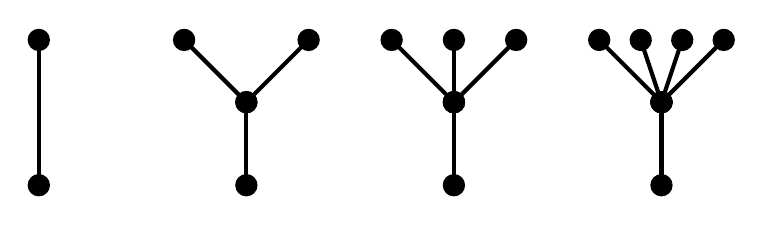
\begin{tikzpicture}[x=0.75pt,y=0.75pt,yscale=-1,xscale=1]
%uncomment if require: \path (0,419); %set diagram left start at 0, and has height of 419

%Straight Lines [id:da7863057024778404] 
\draw [line width=1.5]    (120,130) -- (120,102) -- (120,60) ;
\draw [shift={(120,60)}, rotate = 270] [color={rgb, 255:red, 0; green, 0; blue, 0 }  ][fill={rgb, 255:red, 0; green, 0; blue, 0 }  ][line width=1.5]      (0, 0) circle [x radius= 4.36, y radius= 4.36]   ;
\draw [shift={(120,130)}, rotate = 270] [color={rgb, 255:red, 0; green, 0; blue, 0 }  ][fill={rgb, 255:red, 0; green, 0; blue, 0 }  ][line width=1.5]      (0, 0) circle [x radius= 4.36, y radius= 4.36]   ;
%Straight Lines [id:da3527709376157697] 
\draw [line width=1.5]    (190,60) -- (220,90) ;
\draw [shift={(220,90)}, rotate = 45] [color={rgb, 255:red, 0; green, 0; blue, 0 }  ][fill={rgb, 255:red, 0; green, 0; blue, 0 }  ][line width=1.5]      (0, 0) circle [x radius= 4.36, y radius= 4.36]   ;
\draw [shift={(190,60)}, rotate = 45] [color={rgb, 255:red, 0; green, 0; blue, 0 }  ][fill={rgb, 255:red, 0; green, 0; blue, 0 }  ][line width=1.5]      (0, 0) circle [x radius= 4.36, y radius= 4.36]   ;
%Straight Lines [id:da5026094070566995] 
\draw [line width=1.5]    (220,90) -- (250,60) ;
\draw [shift={(250,60)}, rotate = 315] [color={rgb, 255:red, 0; green, 0; blue, 0 }  ][fill={rgb, 255:red, 0; green, 0; blue, 0 }  ][line width=1.5]      (0, 0) circle [x radius= 4.36, y radius= 4.36]   ;
%Straight Lines [id:da49384351285853745] 
\draw [line width=1.5]    (220,130) -- (220,90) ;
\draw [shift={(220,90)}, rotate = 270] [color={rgb, 255:red, 0; green, 0; blue, 0 }  ][fill={rgb, 255:red, 0; green, 0; blue, 0 }  ][line width=1.5]      (0, 0) circle [x radius= 4.36, y radius= 4.36]   ;
\draw [shift={(220,130)}, rotate = 270] [color={rgb, 255:red, 0; green, 0; blue, 0 }  ][fill={rgb, 255:red, 0; green, 0; blue, 0 }  ][line width=1.5]      (0, 0) circle [x radius= 4.36, y radius= 4.36]   ;
%Straight Lines [id:da4025202167828019] 
\draw [line width=1.5]    (290,60) -- (320,90) ;
\draw [shift={(320,90)}, rotate = 45] [color={rgb, 255:red, 0; green, 0; blue, 0 }  ][fill={rgb, 255:red, 0; green, 0; blue, 0 }  ][line width=1.5]      (0, 0) circle [x radius= 4.36, y radius= 4.36]   ;
\draw [shift={(290,60)}, rotate = 45] [color={rgb, 255:red, 0; green, 0; blue, 0 }  ][fill={rgb, 255:red, 0; green, 0; blue, 0 }  ][line width=1.5]      (0, 0) circle [x radius= 4.36, y radius= 4.36]   ;
%Straight Lines [id:da1762723390926908] 
\draw [line width=1.5]    (320,90) -- (350,60) ;
\draw [shift={(350,60)}, rotate = 315] [color={rgb, 255:red, 0; green, 0; blue, 0 }  ][fill={rgb, 255:red, 0; green, 0; blue, 0 }  ][line width=1.5]      (0, 0) circle [x radius= 4.36, y radius= 4.36]   ;
%Straight Lines [id:da426516312690572] 
\draw [line width=1.5]    (320,130) -- (320,90) ;
\draw [shift={(320,90)}, rotate = 270] [color={rgb, 255:red, 0; green, 0; blue, 0 }  ][fill={rgb, 255:red, 0; green, 0; blue, 0 }  ][line width=1.5]      (0, 0) circle [x radius= 4.36, y radius= 4.36]   ;
\draw [shift={(320,130)}, rotate = 270] [color={rgb, 255:red, 0; green, 0; blue, 0 }  ][fill={rgb, 255:red, 0; green, 0; blue, 0 }  ][line width=1.5]      (0, 0) circle [x radius= 4.36, y radius= 4.36]   ;
%Straight Lines [id:da25638621797362715] 
\draw [line width=1.5]    (390,60) -- (420,90) ;
\draw [shift={(420,90)}, rotate = 45] [color={rgb, 255:red, 0; green, 0; blue, 0 }  ][fill={rgb, 255:red, 0; green, 0; blue, 0 }  ][line width=1.5]      (0, 0) circle [x radius= 4.36, y radius= 4.36]   ;
\draw [shift={(390,60)}, rotate = 45] [color={rgb, 255:red, 0; green, 0; blue, 0 }  ][fill={rgb, 255:red, 0; green, 0; blue, 0 }  ][line width=1.5]      (0, 0) circle [x radius= 4.36, y radius= 4.36]   ;
%Straight Lines [id:da44171571517014097] 
\draw [line width=1.5]    (420,90) -- (450,60) ;
\draw [shift={(450,60)}, rotate = 315] [color={rgb, 255:red, 0; green, 0; blue, 0 }  ][fill={rgb, 255:red, 0; green, 0; blue, 0 }  ][line width=1.5]      (0, 0) circle [x radius= 4.36, y radius= 4.36]   ;
%Straight Lines [id:da05493894156577439] 
\draw [line width=1.5]    (420,130) -- (420,90) ;
\draw [shift={(420,90)}, rotate = 270] [color={rgb, 255:red, 0; green, 0; blue, 0 }  ][fill={rgb, 255:red, 0; green, 0; blue, 0 }  ][line width=1.5]      (0, 0) circle [x radius= 4.36, y radius= 4.36]   ;
\draw [shift={(420,130)}, rotate = 270] [color={rgb, 255:red, 0; green, 0; blue, 0 }  ][fill={rgb, 255:red, 0; green, 0; blue, 0 }  ][line width=1.5]      (0, 0) circle [x radius= 4.36, y radius= 4.36]   ;
%Straight Lines [id:da6858869913750809] 
\draw [line width=1.5]    (320,60) -- (320,90) ;
\draw [shift={(320,90)}, rotate = 90] [color={rgb, 255:red, 0; green, 0; blue, 0 }  ][fill={rgb, 255:red, 0; green, 0; blue, 0 }  ][line width=1.5]      (0, 0) circle [x radius= 4.36, y radius= 4.36]   ;
\draw [shift={(320,60)}, rotate = 90] [color={rgb, 255:red, 0; green, 0; blue, 0 }  ][fill={rgb, 255:red, 0; green, 0; blue, 0 }  ][line width=1.5]      (0, 0) circle [x radius= 4.36, y radius= 4.36]   ;
%Straight Lines [id:da8443523560205857] 
\draw [line width=1.5]    (430,60) -- (420,90) ;
\draw [shift={(420,90)}, rotate = 108.43] [color={rgb, 255:red, 0; green, 0; blue, 0 }  ][fill={rgb, 255:red, 0; green, 0; blue, 0 }  ][line width=1.5]      (0, 0) circle [x radius= 4.36, y radius= 4.36]   ;
\draw [shift={(430,60)}, rotate = 108.43] [color={rgb, 255:red, 0; green, 0; blue, 0 }  ][fill={rgb, 255:red, 0; green, 0; blue, 0 }  ][line width=1.5]      (0, 0) circle [x radius= 4.36, y radius= 4.36]   ;
%Straight Lines [id:da17678730528828934] 
\draw [line width=1.5]    (410,60) -- (420,90) ;
\draw [shift={(420,90)}, rotate = 71.57] [color={rgb, 255:red, 0; green, 0; blue, 0 }  ][fill={rgb, 255:red, 0; green, 0; blue, 0 }  ][line width=1.5]      (0, 0) circle [x radius= 4.36, y radius= 4.36]   ;
\draw [shift={(410,60)}, rotate = 71.57] [color={rgb, 255:red, 0; green, 0; blue, 0 }  ][fill={rgb, 255:red, 0; green, 0; blue, 0 }  ][line width=1.5]      (0, 0) circle [x radius= 4.36, y radius= 4.36]   ;
\end{tikzpicture}    
\end{center}


We can then let these trees interact in certain ways in order to produce the relations we defined an $\A$-algebra by. Lets start with $n=1$. This relation is given by $m_1 m_1=0$, which we can describe with the following rooted tree


% The rooted tree relation describing the first Stasheff identity

\begin{center}
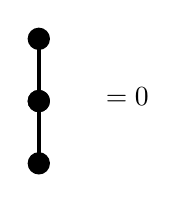
\begin{tikzpicture}[x=0.75pt,y=0.75pt,yscale=-1,xscale=1]
%uncomment if require: \path (0,300); %set diagram left start at 0, and has height of 300

%Straight Lines [id:da5019380442854864] 
\draw [line width=1.5]    (150,180) -- (150,150) ;
\draw [shift={(150,150)}, rotate = 270] [color={rgb, 255:red, 0; green, 0; blue, 0 }  ][fill={rgb, 255:red, 0; green, 0; blue, 0 }  ][line width=1.5]      (0, 0) circle [x radius= 4.36, y radius= 4.36]   ;
\draw [shift={(150,180)}, rotate = 270] [color={rgb, 255:red, 0; green, 0; blue, 0 }  ][fill={rgb, 255:red, 0; green, 0; blue, 0 }  ][line width=1.5]      (0, 0) circle [x radius= 4.36, y radius= 4.36]   ;
%Straight Lines [id:da19340736805161174] 
\draw [line width=1.5]    (150,150) -- (150,120) ;
\draw [shift={(150,120)}, rotate = 270] [color={rgb, 255:red, 0; green, 0; blue, 0 }  ][fill={rgb, 255:red, 0; green, 0; blue, 0 }  ][line width=1.5]      (0, 0) circle [x radius= 4.36, y radius= 4.36]   ;
\draw [shift={(150,150)}, rotate = 270] [color={rgb, 255:red, 0; green, 0; blue, 0 }  ][fill={rgb, 255:red, 0; green, 0; blue, 0 }  ][line width=1.5]      (0, 0) circle [x radius= 4.36, y radius= 4.36]   ;

\draw (181,142.4) node [anchor=north west][inner sep=0.75pt]    {$=0$};

\end{tikzpicture}
\end{center}

Here we have stacked them on top of each other in order to signify that they happen ``after'' each other. We still read from top to bottom, which means that we first do $m_1$, and then $m_1$ again. Note that this rooted tree is the unique way of combining two operations such that the combination is an operation that takes in one element and produces again one element. 

For $n=2$ we have a sum consisting of more then just one element, hence the relation is described by a sum of rooted trees instead. The second relation looks at ways to combine two operations in order to form an operation that takes in two elements and produces just one element. There are three ways of doing this, represented by the following three rooted trees:

% Describing the different ways of combining two trees to get two inputs


\begin{center}
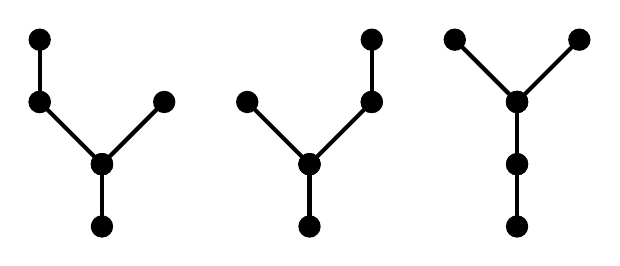
\begin{tikzpicture}[x=0.75pt,y=0.75pt,yscale=-1,xscale=1]
%uncomment if require: \path (0,300); %set diagram left start at 0, and has height of 300

%Straight Lines [id:da8814852158143938] 
\draw [line width=1.5]    (170,180) -- (140,150) ;
\draw [shift={(140,150)}, rotate = 225] [color={rgb, 255:red, 0; green, 0; blue, 0 }  ][fill={rgb, 255:red, 0; green, 0; blue, 0 }  ][line width=1.5]      (0, 0) circle [x radius= 4.36, y radius= 4.36]   ;
\draw [shift={(170,180)}, rotate = 225] [color={rgb, 255:red, 0; green, 0; blue, 0 }  ][fill={rgb, 255:red, 0; green, 0; blue, 0 }  ][line width=1.5]      (0, 0) circle [x radius= 4.36, y radius= 4.36]   ;
%Straight Lines [id:da11602747759122667] 
\draw [line width=1.5]    (140,150) -- (140,120) ;
\draw [shift={(140,120)}, rotate = 270] [color={rgb, 255:red, 0; green, 0; blue, 0 }  ][fill={rgb, 255:red, 0; green, 0; blue, 0 }  ][line width=1.5]      (0, 0) circle [x radius= 4.36, y radius= 4.36]   ;
\draw [shift={(140,150)}, rotate = 270] [color={rgb, 255:red, 0; green, 0; blue, 0 }  ][fill={rgb, 255:red, 0; green, 0; blue, 0 }  ][line width=1.5]      (0, 0) circle [x radius= 4.36, y radius= 4.36]   ;
%Straight Lines [id:da680545812820597] 
\draw [line width=1.5]    (170,180) -- (200,150) ;
\draw [shift={(200,150)}, rotate = 315] [color={rgb, 255:red, 0; green, 0; blue, 0 }  ][fill={rgb, 255:red, 0; green, 0; blue, 0 }  ][line width=1.5]      (0, 0) circle [x radius= 4.36, y radius= 4.36]   ;
\draw [shift={(170,180)}, rotate = 315] [color={rgb, 255:red, 0; green, 0; blue, 0 }  ][fill={rgb, 255:red, 0; green, 0; blue, 0 }  ][line width=1.5]      (0, 0) circle [x radius= 4.36, y radius= 4.36]   ;
%Straight Lines [id:da614958153258419] 
\draw [line width=1.5]    (170,210) -- (170,180) ;
\draw [shift={(170,180)}, rotate = 270] [color={rgb, 255:red, 0; green, 0; blue, 0 }  ][fill={rgb, 255:red, 0; green, 0; blue, 0 }  ][line width=1.5]      (0, 0) circle [x radius= 4.36, y radius= 4.36]   ;
\draw [shift={(170,210)}, rotate = 270] [color={rgb, 255:red, 0; green, 0; blue, 0 }  ][fill={rgb, 255:red, 0; green, 0; blue, 0 }  ][line width=1.5]      (0, 0) circle [x radius= 4.36, y radius= 4.36]   ;
%Straight Lines [id:da2890370558484694] 
\draw [line width=1.5]    (270,180) -- (240,150) ;
\draw [shift={(240,150)}, rotate = 225] [color={rgb, 255:red, 0; green, 0; blue, 0 }  ][fill={rgb, 255:red, 0; green, 0; blue, 0 }  ][line width=1.5]      (0, 0) circle [x radius= 4.36, y radius= 4.36]   ;
\draw [shift={(270,180)}, rotate = 225] [color={rgb, 255:red, 0; green, 0; blue, 0 }  ][fill={rgb, 255:red, 0; green, 0; blue, 0 }  ][line width=1.5]      (0, 0) circle [x radius= 4.36, y radius= 4.36]   ;
%Straight Lines [id:da36602089442829633] 
\draw [line width=1.5]    (300,150) -- (300,120) ;
\draw [shift={(300,120)}, rotate = 270] [color={rgb, 255:red, 0; green, 0; blue, 0 }  ][fill={rgb, 255:red, 0; green, 0; blue, 0 }  ][line width=1.5]      (0, 0) circle [x radius= 4.36, y radius= 4.36]   ;
\draw [shift={(300,150)}, rotate = 270] [color={rgb, 255:red, 0; green, 0; blue, 0 }  ][fill={rgb, 255:red, 0; green, 0; blue, 0 }  ][line width=1.5]      (0, 0) circle [x radius= 4.36, y radius= 4.36]   ;
%Straight Lines [id:da7885321218362338] 
\draw [line width=1.5]    (270,180) -- (300,150) ;
\draw [shift={(300,150)}, rotate = 315] [color={rgb, 255:red, 0; green, 0; blue, 0 }  ][fill={rgb, 255:red, 0; green, 0; blue, 0 }  ][line width=1.5]      (0, 0) circle [x radius= 4.36, y radius= 4.36]   ;
\draw [shift={(270,180)}, rotate = 315] [color={rgb, 255:red, 0; green, 0; blue, 0 }  ][fill={rgb, 255:red, 0; green, 0; blue, 0 }  ][line width=1.5]      (0, 0) circle [x radius= 4.36, y radius= 4.36]   ;
%Straight Lines [id:da9545027465587088] 
\draw [line width=1.5]    (270,210) -- (270,180) ;
\draw [shift={(270,180)}, rotate = 270] [color={rgb, 255:red, 0; green, 0; blue, 0 }  ][fill={rgb, 255:red, 0; green, 0; blue, 0 }  ][line width=1.5]      (0, 0) circle [x radius= 4.36, y radius= 4.36]   ;
\draw [shift={(270,210)}, rotate = 270] [color={rgb, 255:red, 0; green, 0; blue, 0 }  ][fill={rgb, 255:red, 0; green, 0; blue, 0 }  ][line width=1.5]      (0, 0) circle [x radius= 4.36, y radius= 4.36]   ;
%Straight Lines [id:da07994174288427436] 
\draw [line width=1.5]    (370,150) -- (340,120) ;
\draw [shift={(340,120)}, rotate = 225] [color={rgb, 255:red, 0; green, 0; blue, 0 }  ][fill={rgb, 255:red, 0; green, 0; blue, 0 }  ][line width=1.5]      (0, 0) circle [x radius= 4.36, y radius= 4.36]   ;
\draw [shift={(370,150)}, rotate = 225] [color={rgb, 255:red, 0; green, 0; blue, 0 }  ][fill={rgb, 255:red, 0; green, 0; blue, 0 }  ][line width=1.5]      (0, 0) circle [x radius= 4.36, y radius= 4.36]   ;
%Straight Lines [id:da5019380442854864] 
\draw [line width=1.5]    (370,210) -- (370,180) ;
\draw [shift={(370,180)}, rotate = 270] [color={rgb, 255:red, 0; green, 0; blue, 0 }  ][fill={rgb, 255:red, 0; green, 0; blue, 0 }  ][line width=1.5]      (0, 0) circle [x radius= 4.36, y radius= 4.36]   ;
\draw [shift={(370,210)}, rotate = 270] [color={rgb, 255:red, 0; green, 0; blue, 0 }  ][fill={rgb, 255:red, 0; green, 0; blue, 0 }  ][line width=1.5]      (0, 0) circle [x radius= 4.36, y radius= 4.36]   ;
%Straight Lines [id:da16295370354613858] 
\draw [line width=1.5]    (370,150) -- (400,120) ;
\draw [shift={(400,120)}, rotate = 315] [color={rgb, 255:red, 0; green, 0; blue, 0 }  ][fill={rgb, 255:red, 0; green, 0; blue, 0 }  ][line width=1.5]      (0, 0) circle [x radius= 4.36, y radius= 4.36]   ;
\draw [shift={(370,150)}, rotate = 315] [color={rgb, 255:red, 0; green, 0; blue, 0 }  ][fill={rgb, 255:red, 0; green, 0; blue, 0 }  ][line width=1.5]      (0, 0) circle [x radius= 4.36, y radius= 4.36]   ;
%Straight Lines [id:da19340736805161174] 
\draw [line width=1.5]    (370,180) -- (370,150) ;
\draw [shift={(370,150)}, rotate = 270] [color={rgb, 255:red, 0; green, 0; blue, 0 }  ][fill={rgb, 255:red, 0; green, 0; blue, 0 }  ][line width=1.5]      (0, 0) circle [x radius= 4.36, y radius= 4.36]   ;
\draw [shift={(370,180)}, rotate = 270] [color={rgb, 255:red, 0; green, 0; blue, 0 }  ][fill={rgb, 255:red, 0; green, 0; blue, 0 }  ][line width=1.5]      (0, 0) circle [x radius= 4.36, y radius= 4.36]   ;
\end{tikzpicture}    
\end{center}

Note here that we have omitted the identity maps which should be present. If we add these we get for example the following:

% Describing the omittance of identity maps in the drawings

\begin{center}
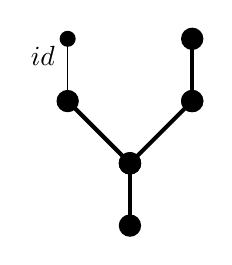
\begin{tikzpicture}[x=0.75pt,y=0.75pt,yscale=-1,xscale=1]
%uncomment if require: \path (0,300); %set diagram left start at 0, and has height of 300

%Straight Lines [id:da3941708866613911] 
\draw [line width=1.5]    (220,140) -- (190,110) ;
\draw [shift={(190,110)}, rotate = 225] [color={rgb, 255:red, 0; green, 0; blue, 0 }  ][fill={rgb, 255:red, 0; green, 0; blue, 0 }  ][line width=1.5]      (0, 0) circle [x radius= 4.36, y radius= 4.36]   ;
\draw [shift={(220,140)}, rotate = 225] [color={rgb, 255:red, 0; green, 0; blue, 0 }  ][fill={rgb, 255:red, 0; green, 0; blue, 0 }  ][line width=1.5]      (0, 0) circle [x radius= 4.36, y radius= 4.36]   ;
%Straight Lines [id:da300120384085371] 
\draw [line width=1.5]    (220,140) -- (250,110) ;
\draw [shift={(250,110)}, rotate = 315] [color={rgb, 255:red, 0; green, 0; blue, 0 }  ][fill={rgb, 255:red, 0; green, 0; blue, 0 }  ][line width=1.5]      (0, 0) circle [x radius= 4.36, y radius= 4.36]   ;
\draw [shift={(220,140)}, rotate = 315] [color={rgb, 255:red, 0; green, 0; blue, 0 }  ][fill={rgb, 255:red, 0; green, 0; blue, 0 }  ][line width=1.5]      (0, 0) circle [x radius= 4.36, y radius= 4.36]   ;
%Straight Lines [id:da14962304311021435] 
\draw [line width=1.5]    (220,170) -- (220,140) ;
\draw [shift={(220,140)}, rotate = 270] [color={rgb, 255:red, 0; green, 0; blue, 0 }  ][fill={rgb, 255:red, 0; green, 0; blue, 0 }  ][line width=1.5]      (0, 0) circle [x radius= 4.36, y radius= 4.36]   ;
\draw [shift={(220,170)}, rotate = 270] [color={rgb, 255:red, 0; green, 0; blue, 0 }  ][fill={rgb, 255:red, 0; green, 0; blue, 0 }  ][line width=1.5]      (0, 0) circle [x radius= 4.36, y radius= 4.36]   ;
%Straight Lines [id:da41279118247571556] 
\draw [line width=1.5]    (250,110) -- (250,80) ;
\draw [shift={(250,80)}, rotate = 270] [color={rgb, 255:red, 0; green, 0; blue, 0 }  ][fill={rgb, 255:red, 0; green, 0; blue, 0 }  ][line width=1.5]      (0, 0) circle [x radius= 4.36, y radius= 4.36]   ;
\draw [shift={(250,110)}, rotate = 270] [color={rgb, 255:red, 0; green, 0; blue, 0 }  ][fill={rgb, 255:red, 0; green, 0; blue, 0 }  ][line width=1.5]      (0, 0) circle [x radius= 4.36, y radius= 4.36]   ;
%Straight Lines [id:da9592865880987089] 
\draw    (190,80) -- (190,110) ;
\draw [shift={(190,80)}, rotate = 90] [color={rgb, 255:red, 0; green, 0; blue, 0 }  ][fill={rgb, 255:red, 0; green, 0; blue, 0 }  ][line width=0.75]      (0, 0) circle [x radius= 3.35, y radius= 3.35]   ;

% Text Node
\draw (171,82.4) node [anchor=north west][inner sep=0.75pt]    {$id$};


\end{tikzpicture}    
\end{center}

For simplicity we omit these identities, as they add a bit of confusion because of their similarity to the $m_1$ operation. So whenever one sees one operation starting lower than another, add identities to get to the same height.

In order to produce the second Stasheff identity we need to add these together in the correct way. This correct way, as calculated earlier, is the following:

% Second Stasheff identity using trees, with signs



\begin{center}
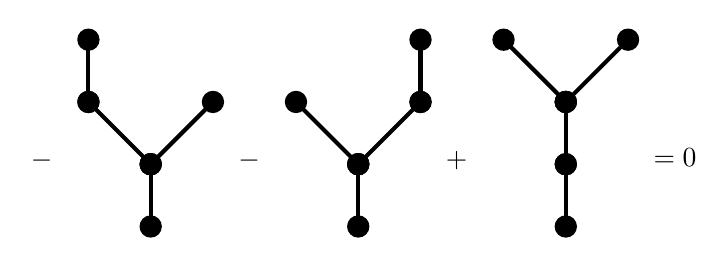
\begin{tikzpicture}[x=0.75pt,y=0.75pt,yscale=-1,xscale=1]
%uncomment if require: \path (0,300); %set diagram left start at 0, and has height of 300

%Straight Lines [id:da31477124000159296] 
\draw [line width=1.5]    (120,140) -- (90,110) ;
\draw [shift={(90,110)}, rotate = 225] [color={rgb, 255:red, 0; green, 0; blue, 0 }  ][fill={rgb, 255:red, 0; green, 0; blue, 0 }  ][line width=1.5]      (0, 0) circle [x radius= 4.36, y radius= 4.36]   ;
\draw [shift={(120,140)}, rotate = 225] [color={rgb, 255:red, 0; green, 0; blue, 0 }  ][fill={rgb, 255:red, 0; green, 0; blue, 0 }  ][line width=1.5]      (0, 0) circle [x radius= 4.36, y radius= 4.36]   ;
%Straight Lines [id:da49139183729214175] 
\draw [line width=1.5]    (120,140) -- (150,110) ;
\draw [shift={(150,110)}, rotate = 315] [color={rgb, 255:red, 0; green, 0; blue, 0 }  ][fill={rgb, 255:red, 0; green, 0; blue, 0 }  ][line width=1.5]      (0, 0) circle [x radius= 4.36, y radius= 4.36]   ;
\draw [shift={(120,140)}, rotate = 315] [color={rgb, 255:red, 0; green, 0; blue, 0 }  ][fill={rgb, 255:red, 0; green, 0; blue, 0 }  ][line width=1.5]      (0, 0) circle [x radius= 4.36, y radius= 4.36]   ;
%Straight Lines [id:da49681202435755245] 
\draw [line width=1.5]    (120,170) -- (120,140) ;
\draw [shift={(120,140)}, rotate = 270] [color={rgb, 255:red, 0; green, 0; blue, 0 }  ][fill={rgb, 255:red, 0; green, 0; blue, 0 }  ][line width=1.5]      (0, 0) circle [x radius= 4.36, y radius= 4.36]   ;
\draw [shift={(120,170)}, rotate = 270] [color={rgb, 255:red, 0; green, 0; blue, 0 }  ][fill={rgb, 255:red, 0; green, 0; blue, 0 }  ][line width=1.5]      (0, 0) circle [x radius= 4.36, y radius= 4.36]   ;
%Straight Lines [id:da3941708866613911] 
\draw [line width=1.5]    (220,140) -- (190,110) ;
\draw [shift={(190,110)}, rotate = 225] [color={rgb, 255:red, 0; green, 0; blue, 0 }  ][fill={rgb, 255:red, 0; green, 0; blue, 0 }  ][line width=1.5]      (0, 0) circle [x radius= 4.36, y radius= 4.36]   ;
\draw [shift={(220,140)}, rotate = 225] [color={rgb, 255:red, 0; green, 0; blue, 0 }  ][fill={rgb, 255:red, 0; green, 0; blue, 0 }  ][line width=1.5]      (0, 0) circle [x radius= 4.36, y radius= 4.36]   ;
%Straight Lines [id:da300120384085371] 
\draw [line width=1.5]    (220,140) -- (250,110) ;
\draw [shift={(250,110)}, rotate = 315] [color={rgb, 255:red, 0; green, 0; blue, 0 }  ][fill={rgb, 255:red, 0; green, 0; blue, 0 }  ][line width=1.5]      (0, 0) circle [x radius= 4.36, y radius= 4.36]   ;
\draw [shift={(220,140)}, rotate = 315] [color={rgb, 255:red, 0; green, 0; blue, 0 }  ][fill={rgb, 255:red, 0; green, 0; blue, 0 }  ][line width=1.5]      (0, 0) circle [x radius= 4.36, y radius= 4.36]   ;
%Straight Lines [id:da14962304311021435] 
\draw [line width=1.5]    (220,170) -- (220,140) ;
\draw [shift={(220,140)}, rotate = 270] [color={rgb, 255:red, 0; green, 0; blue, 0 }  ][fill={rgb, 255:red, 0; green, 0; blue, 0 }  ][line width=1.5]      (0, 0) circle [x radius= 4.36, y radius= 4.36]   ;
\draw [shift={(220,170)}, rotate = 270] [color={rgb, 255:red, 0; green, 0; blue, 0 }  ][fill={rgb, 255:red, 0; green, 0; blue, 0 }  ][line width=1.5]      (0, 0) circle [x radius= 4.36, y radius= 4.36]   ;
%Straight Lines [id:da6955709488854369] 
\draw [line width=1.5]    (320,110) -- (290,80) ;
\draw [shift={(290,80)}, rotate = 225] [color={rgb, 255:red, 0; green, 0; blue, 0 }  ][fill={rgb, 255:red, 0; green, 0; blue, 0 }  ][line width=1.5]      (0, 0) circle [x radius= 4.36, y radius= 4.36]   ;
\draw [shift={(320,110)}, rotate = 225] [color={rgb, 255:red, 0; green, 0; blue, 0 }  ][fill={rgb, 255:red, 0; green, 0; blue, 0 }  ][line width=1.5]      (0, 0) circle [x radius= 4.36, y radius= 4.36]   ;
%Straight Lines [id:da11504103913241726] 
\draw [line width=1.5]    (320,110) -- (350,80) ;
\draw [shift={(350,80)}, rotate = 315] [color={rgb, 255:red, 0; green, 0; blue, 0 }  ][fill={rgb, 255:red, 0; green, 0; blue, 0 }  ][line width=1.5]      (0, 0) circle [x radius= 4.36, y radius= 4.36]   ;
\draw [shift={(320,110)}, rotate = 315] [color={rgb, 255:red, 0; green, 0; blue, 0 }  ][fill={rgb, 255:red, 0; green, 0; blue, 0 }  ][line width=1.5]      (0, 0) circle [x radius= 4.36, y radius= 4.36]   ;
%Straight Lines [id:da004089317473789711] 
\draw [line width=1.5]    (320,140) -- (320,110) ;
\draw [shift={(320,110)}, rotate = 270] [color={rgb, 255:red, 0; green, 0; blue, 0 }  ][fill={rgb, 255:red, 0; green, 0; blue, 0 }  ][line width=1.5]      (0, 0) circle [x radius= 4.36, y radius= 4.36]   ;
\draw [shift={(320,140)}, rotate = 270] [color={rgb, 255:red, 0; green, 0; blue, 0 }  ][fill={rgb, 255:red, 0; green, 0; blue, 0 }  ][line width=1.5]      (0, 0) circle [x radius= 4.36, y radius= 4.36]   ;
%Straight Lines [id:da8569365387106636] 
\draw [line width=1.5]    (90,110) -- (90,80) ;
\draw [shift={(90,80)}, rotate = 270] [color={rgb, 255:red, 0; green, 0; blue, 0 }  ][fill={rgb, 255:red, 0; green, 0; blue, 0 }  ][line width=1.5]      (0, 0) circle [x radius= 4.36, y radius= 4.36]   ;
\draw [shift={(90,110)}, rotate = 270] [color={rgb, 255:red, 0; green, 0; blue, 0 }  ][fill={rgb, 255:red, 0; green, 0; blue, 0 }  ][line width=1.5]      (0, 0) circle [x radius= 4.36, y radius= 4.36]   ;
%Straight Lines [id:da41279118247571556] 
\draw [line width=1.5]    (250,110) -- (250,80) ;
\draw [shift={(250,80)}, rotate = 270] [color={rgb, 255:red, 0; green, 0; blue, 0 }  ][fill={rgb, 255:red, 0; green, 0; blue, 0 }  ][line width=1.5]      (0, 0) circle [x radius= 4.36, y radius= 4.36]   ;
\draw [shift={(250,110)}, rotate = 270] [color={rgb, 255:red, 0; green, 0; blue, 0 }  ][fill={rgb, 255:red, 0; green, 0; blue, 0 }  ][line width=1.5]      (0, 0) circle [x radius= 4.36, y radius= 4.36]   ;
%Straight Lines [id:da5701552758066648] 
\draw [line width=1.5]    (320,170) -- (320,140) ;
\draw [shift={(320,140)}, rotate = 270] [color={rgb, 255:red, 0; green, 0; blue, 0 }  ][fill={rgb, 255:red, 0; green, 0; blue, 0 }  ][line width=1.5]      (0, 0) circle [x radius= 4.36, y radius= 4.36]   ;
\draw [shift={(320,170)}, rotate = 270] [color={rgb, 255:red, 0; green, 0; blue, 0 }  ][fill={rgb, 255:red, 0; green, 0; blue, 0 }  ][line width=1.5]      (0, 0) circle [x radius= 4.36, y radius= 4.36]   ;

% Text Node
\draw (361,131.4) node [anchor=north west][inner sep=0.75pt]    {$=0$};
% Text Node
\draw (61,132.4) node [anchor=north west][inner sep=0.75pt]    {$-$};
% Text Node
\draw (161,132.4) node [anchor=north west][inner sep=0.75pt]    {$-$};
% Text Node
\draw (261,132.4) node [anchor=north west][inner sep=0.75pt]    {$+$};


\end{tikzpicture}    
\end{center}

We can figure out the correct signs by looking at the $r, s, t$ decomposition of $n$. For this particular example, when $n=2$ we have three decompositions
\begin{itemize}
    \item $r=0, s=1, t=1$
    \item $r=1, s=1, t=0$
    \item $r=0, s=2, t=0$
\end{itemize}
These are the ingredients in the sign $(-1)^{r+st}$ which we have in the Stasheff identities. The integer $s$ denotes the operation $m_s$ we will see at the top of the rooted tree. The integer $r$ denotes the position of this top operation, i.e. how far to the right it will be placed on the leaves of the operation at the bottom. The bottom operation will be given by $r+1+t$, i.e. $m_{r+1+t}$. This means that we can read of the correct sign from the composed rooted tree of the two operations, as the placements of the sub-trees from the top operation completely determines it. Let's see an example of how we can read out the signs. We have

% Describing how to read off the correct sign from the tree



\begin{center}
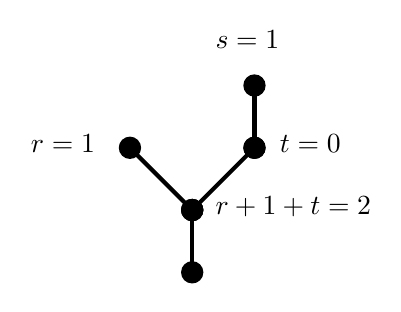
\begin{tikzpicture}[x=0.75pt,y=0.75pt,yscale=-1,xscale=1]
%uncomment if require: \path (0,300); %set diagram left start at 0, and has height of 300

%Straight Lines [id:da3941708866613911] 
\draw [line width=1.5]    (220,140) -- (190,110) ;
\draw [shift={(190,110)}, rotate = 225] [color={rgb, 255:red, 0; green, 0; blue, 0 }  ][fill={rgb, 255:red, 0; green, 0; blue, 0 }  ][line width=1.5]      (0, 0) circle [x radius= 4.36, y radius= 4.36]   ;
\draw [shift={(220,140)}, rotate = 225] [color={rgb, 255:red, 0; green, 0; blue, 0 }  ][fill={rgb, 255:red, 0; green, 0; blue, 0 }  ][line width=1.5]      (0, 0) circle [x radius= 4.36, y radius= 4.36]   ;
%Straight Lines [id:da300120384085371] 
\draw [line width=1.5]    (220,140) -- (250,110) ;
\draw [shift={(250,110)}, rotate = 315] [color={rgb, 255:red, 0; green, 0; blue, 0 }  ][fill={rgb, 255:red, 0; green, 0; blue, 0 }  ][line width=1.5]      (0, 0) circle [x radius= 4.36, y radius= 4.36]   ;
\draw [shift={(220,140)}, rotate = 315] [color={rgb, 255:red, 0; green, 0; blue, 0 }  ][fill={rgb, 255:red, 0; green, 0; blue, 0 }  ][line width=1.5]      (0, 0) circle [x radius= 4.36, y radius= 4.36]   ;
%Straight Lines [id:da14962304311021435] 
\draw [line width=1.5]    (220,170) -- (220,140) ;
\draw [shift={(220,140)}, rotate = 270] [color={rgb, 255:red, 0; green, 0; blue, 0 }  ][fill={rgb, 255:red, 0; green, 0; blue, 0 }  ][line width=1.5]      (0, 0) circle [x radius= 4.36, y radius= 4.36]   ;
\draw [shift={(220,170)}, rotate = 270] [color={rgb, 255:red, 0; green, 0; blue, 0 }  ][fill={rgb, 255:red, 0; green, 0; blue, 0 }  ][line width=1.5]      (0, 0) circle [x radius= 4.36, y radius= 4.36]   ;
%Straight Lines [id:da41279118247571556] 
\draw [line width=1.5]    (250,110) -- (250,80) ;
\draw [shift={(250,80)}, rotate = 270] [color={rgb, 255:red, 0; green, 0; blue, 0 }  ][fill={rgb, 255:red, 0; green, 0; blue, 0 }  ][line width=1.5]      (0, 0) circle [x radius= 4.36, y radius= 4.36]   ;
\draw [shift={(250,110)}, rotate = 270] [color={rgb, 255:red, 0; green, 0; blue, 0 }  ][fill={rgb, 255:red, 0; green, 0; blue, 0 }  ][line width=1.5]      (0, 0) circle [x radius= 4.36, y radius= 4.36]   ;

% Text Node
\draw (141,102.4) node [anchor=north west][inner sep=0.75pt]    {$r=1$};
% Text Node
\draw (261,102.4) node [anchor=north west][inner sep=0.75pt]    {$t=0$};
% Text Node
\draw (230,52.4) node [anchor=north west][inner sep=0.75pt]    {$s=1$};
% Text Node
\draw (230,132.4) node [anchor=north west][inner sep=0.75pt]    {$r+1+t=2$};

\end{tikzpicture}
\end{center}

which means that the correct associated sign is $(-1)^{r+st}=(-1)^{1+1\cdot 0}=(-1)$. 





One way to create the correct system of trees for some  $n$ with the correct signs is the following. 
\begin{enumerate}
    \item Draw $n$ copies of the rooted tree that represents $m_n$. 
    \item Put one copy of the binary tree that represents $m_1$ at each of the leaves of the above copies of $m_n$ by first putting it on the leftmost one and then continuing to the right. 
\end{enumerate}
This is easier by a visualization, so let $n=4$. Then by doing the above two steps we get the following:



% Example for trees with four inputs 


\begin{center}
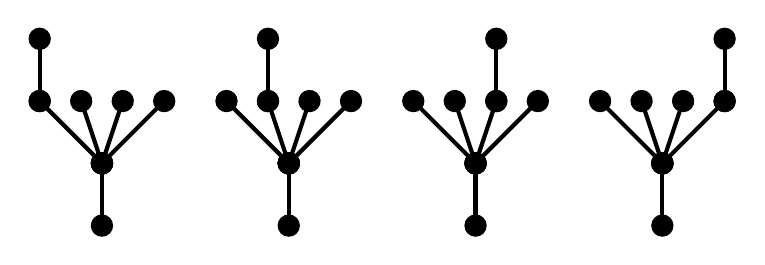
\begin{tikzpicture}[x=0.75pt,y=0.75pt,yscale=-1,xscale=1]
%uncomment if require: \path (0,300); %set diagram left start at 0, and has height of 300

%Straight Lines [id:da7271236022900844] 
\draw [line width=1.5]    (120,120) -- (90,90) ;
\draw [shift={(90,90)}, rotate = 225] [color={rgb, 255:red, 0; green, 0; blue, 0 }  ][fill={rgb, 255:red, 0; green, 0; blue, 0 }  ][line width=1.5]      (0, 0) circle [x radius= 4.36, y radius= 4.36]   ;
\draw [shift={(120,120)}, rotate = 225] [color={rgb, 255:red, 0; green, 0; blue, 0 }  ][fill={rgb, 255:red, 0; green, 0; blue, 0 }  ][line width=1.5]      (0, 0) circle [x radius= 4.36, y radius= 4.36]   ;
%Straight Lines [id:da8829298962249057] 
\draw [line width=1.5]    (120,120) -- (110,90) ;
\draw [shift={(110,90)}, rotate = 251.57] [color={rgb, 255:red, 0; green, 0; blue, 0 }  ][fill={rgb, 255:red, 0; green, 0; blue, 0 }  ][line width=1.5]      (0, 0) circle [x radius= 4.36, y radius= 4.36]   ;
\draw [shift={(120,120)}, rotate = 251.57] [color={rgb, 255:red, 0; green, 0; blue, 0 }  ][fill={rgb, 255:red, 0; green, 0; blue, 0 }  ][line width=1.5]      (0, 0) circle [x radius= 4.36, y radius= 4.36]   ;
%Straight Lines [id:da14019661944022443] 
\draw [line width=1.5]    (120,120) -- (150,90) ;
\draw [shift={(150,90)}, rotate = 315] [color={rgb, 255:red, 0; green, 0; blue, 0 }  ][fill={rgb, 255:red, 0; green, 0; blue, 0 }  ][line width=1.5]      (0, 0) circle [x radius= 4.36, y radius= 4.36]   ;
\draw [shift={(120,120)}, rotate = 315] [color={rgb, 255:red, 0; green, 0; blue, 0 }  ][fill={rgb, 255:red, 0; green, 0; blue, 0 }  ][line width=1.5]      (0, 0) circle [x radius= 4.36, y radius= 4.36]   ;
%Straight Lines [id:da3561053996918748] 
\draw [line width=1.5]    (120,150) -- (120,120) ;
\draw [shift={(120,120)}, rotate = 270] [color={rgb, 255:red, 0; green, 0; blue, 0 }  ][fill={rgb, 255:red, 0; green, 0; blue, 0 }  ][line width=1.5]      (0, 0) circle [x radius= 4.36, y radius= 4.36]   ;
\draw [shift={(120,150)}, rotate = 270] [color={rgb, 255:red, 0; green, 0; blue, 0 }  ][fill={rgb, 255:red, 0; green, 0; blue, 0 }  ][line width=1.5]      (0, 0) circle [x radius= 4.36, y radius= 4.36]   ;
%Straight Lines [id:da12959305658190345] 
\draw [line width=1.5]    (130,90) -- (120,120) ;
\draw [shift={(120,120)}, rotate = 108.43] [color={rgb, 255:red, 0; green, 0; blue, 0 }  ][fill={rgb, 255:red, 0; green, 0; blue, 0 }  ][line width=1.5]      (0, 0) circle [x radius= 4.36, y radius= 4.36]   ;
\draw [shift={(130,90)}, rotate = 108.43] [color={rgb, 255:red, 0; green, 0; blue, 0 }  ][fill={rgb, 255:red, 0; green, 0; blue, 0 }  ][line width=1.5]      (0, 0) circle [x radius= 4.36, y radius= 4.36]   ;
%Straight Lines [id:da17788889705056876] 
\draw [line width=1.5]    (210,120) -- (180,90) ;
\draw [shift={(180,90)}, rotate = 225] [color={rgb, 255:red, 0; green, 0; blue, 0 }  ][fill={rgb, 255:red, 0; green, 0; blue, 0 }  ][line width=1.5]      (0, 0) circle [x radius= 4.36, y radius= 4.36]   ;
\draw [shift={(210,120)}, rotate = 225] [color={rgb, 255:red, 0; green, 0; blue, 0 }  ][fill={rgb, 255:red, 0; green, 0; blue, 0 }  ][line width=1.5]      (0, 0) circle [x radius= 4.36, y radius= 4.36]   ;
%Straight Lines [id:da32726690992182617] 
\draw [line width=1.5]    (210,120) -- (200,90) ;
\draw [shift={(200,90)}, rotate = 251.57] [color={rgb, 255:red, 0; green, 0; blue, 0 }  ][fill={rgb, 255:red, 0; green, 0; blue, 0 }  ][line width=1.5]      (0, 0) circle [x radius= 4.36, y radius= 4.36]   ;
\draw [shift={(210,120)}, rotate = 251.57] [color={rgb, 255:red, 0; green, 0; blue, 0 }  ][fill={rgb, 255:red, 0; green, 0; blue, 0 }  ][line width=1.5]      (0, 0) circle [x radius= 4.36, y radius= 4.36]   ;
%Straight Lines [id:da6529521762459134] 
\draw [line width=1.5]    (210,120) -- (240,90) ;
\draw [shift={(240,90)}, rotate = 315] [color={rgb, 255:red, 0; green, 0; blue, 0 }  ][fill={rgb, 255:red, 0; green, 0; blue, 0 }  ][line width=1.5]      (0, 0) circle [x radius= 4.36, y radius= 4.36]   ;
\draw [shift={(210,120)}, rotate = 315] [color={rgb, 255:red, 0; green, 0; blue, 0 }  ][fill={rgb, 255:red, 0; green, 0; blue, 0 }  ][line width=1.5]      (0, 0) circle [x radius= 4.36, y radius= 4.36]   ;
%Straight Lines [id:da10508941767197344] 
\draw [line width=1.5]    (210,150) -- (210,120) ;
\draw [shift={(210,120)}, rotate = 270] [color={rgb, 255:red, 0; green, 0; blue, 0 }  ][fill={rgb, 255:red, 0; green, 0; blue, 0 }  ][line width=1.5]      (0, 0) circle [x radius= 4.36, y radius= 4.36]   ;
\draw [shift={(210,150)}, rotate = 270] [color={rgb, 255:red, 0; green, 0; blue, 0 }  ][fill={rgb, 255:red, 0; green, 0; blue, 0 }  ][line width=1.5]      (0, 0) circle [x radius= 4.36, y radius= 4.36]   ;
%Straight Lines [id:da6259633442377939] 
\draw [line width=1.5]    (220,90) -- (210,120) ;
\draw [shift={(210,120)}, rotate = 108.43] [color={rgb, 255:red, 0; green, 0; blue, 0 }  ][fill={rgb, 255:red, 0; green, 0; blue, 0 }  ][line width=1.5]      (0, 0) circle [x radius= 4.36, y radius= 4.36]   ;
\draw [shift={(220,90)}, rotate = 108.43] [color={rgb, 255:red, 0; green, 0; blue, 0 }  ][fill={rgb, 255:red, 0; green, 0; blue, 0 }  ][line width=1.5]      (0, 0) circle [x radius= 4.36, y radius= 4.36]   ;
%Straight Lines [id:da18827403823128308] 
\draw [line width=1.5]    (300,120) -- (270,90) ;
\draw [shift={(270,90)}, rotate = 225] [color={rgb, 255:red, 0; green, 0; blue, 0 }  ][fill={rgb, 255:red, 0; green, 0; blue, 0 }  ][line width=1.5]      (0, 0) circle [x radius= 4.36, y radius= 4.36]   ;
\draw [shift={(300,120)}, rotate = 225] [color={rgb, 255:red, 0; green, 0; blue, 0 }  ][fill={rgb, 255:red, 0; green, 0; blue, 0 }  ][line width=1.5]      (0, 0) circle [x radius= 4.36, y radius= 4.36]   ;
%Straight Lines [id:da4416224263321782] 
\draw [line width=1.5]    (300,120) -- (290,90) ;
\draw [shift={(290,90)}, rotate = 251.57] [color={rgb, 255:red, 0; green, 0; blue, 0 }  ][fill={rgb, 255:red, 0; green, 0; blue, 0 }  ][line width=1.5]      (0, 0) circle [x radius= 4.36, y radius= 4.36]   ;
\draw [shift={(300,120)}, rotate = 251.57] [color={rgb, 255:red, 0; green, 0; blue, 0 }  ][fill={rgb, 255:red, 0; green, 0; blue, 0 }  ][line width=1.5]      (0, 0) circle [x radius= 4.36, y radius= 4.36]   ;
%Straight Lines [id:da4912193105487581] 
\draw [line width=1.5]    (300,120) -- (330,90) ;
\draw [shift={(330,90)}, rotate = 315] [color={rgb, 255:red, 0; green, 0; blue, 0 }  ][fill={rgb, 255:red, 0; green, 0; blue, 0 }  ][line width=1.5]      (0, 0) circle [x radius= 4.36, y radius= 4.36]   ;
\draw [shift={(300,120)}, rotate = 315] [color={rgb, 255:red, 0; green, 0; blue, 0 }  ][fill={rgb, 255:red, 0; green, 0; blue, 0 }  ][line width=1.5]      (0, 0) circle [x radius= 4.36, y radius= 4.36]   ;
%Straight Lines [id:da057140828311111225] 
\draw [line width=1.5]    (300,150) -- (300,120) ;
\draw [shift={(300,120)}, rotate = 270] [color={rgb, 255:red, 0; green, 0; blue, 0 }  ][fill={rgb, 255:red, 0; green, 0; blue, 0 }  ][line width=1.5]      (0, 0) circle [x radius= 4.36, y radius= 4.36]   ;
\draw [shift={(300,150)}, rotate = 270] [color={rgb, 255:red, 0; green, 0; blue, 0 }  ][fill={rgb, 255:red, 0; green, 0; blue, 0 }  ][line width=1.5]      (0, 0) circle [x radius= 4.36, y radius= 4.36]   ;
%Straight Lines [id:da6532175337656438] 
\draw [line width=1.5]    (310,90) -- (300,120) ;
\draw [shift={(300,120)}, rotate = 108.43] [color={rgb, 255:red, 0; green, 0; blue, 0 }  ][fill={rgb, 255:red, 0; green, 0; blue, 0 }  ][line width=1.5]      (0, 0) circle [x radius= 4.36, y radius= 4.36]   ;
\draw [shift={(310,90)}, rotate = 108.43] [color={rgb, 255:red, 0; green, 0; blue, 0 }  ][fill={rgb, 255:red, 0; green, 0; blue, 0 }  ][line width=1.5]      (0, 0) circle [x radius= 4.36, y radius= 4.36]   ;
%Straight Lines [id:da9439423309856876] 
\draw [line width=1.5]    (390,120) -- (360,90) ;
\draw [shift={(360,90)}, rotate = 225] [color={rgb, 255:red, 0; green, 0; blue, 0 }  ][fill={rgb, 255:red, 0; green, 0; blue, 0 }  ][line width=1.5]      (0, 0) circle [x radius= 4.36, y radius= 4.36]   ;
\draw [shift={(390,120)}, rotate = 225] [color={rgb, 255:red, 0; green, 0; blue, 0 }  ][fill={rgb, 255:red, 0; green, 0; blue, 0 }  ][line width=1.5]      (0, 0) circle [x radius= 4.36, y radius= 4.36]   ;
%Straight Lines [id:da6793777254659024] 
\draw [line width=1.5]    (390,120) -- (380,90) ;
\draw [shift={(380,90)}, rotate = 251.57] [color={rgb, 255:red, 0; green, 0; blue, 0 }  ][fill={rgb, 255:red, 0; green, 0; blue, 0 }  ][line width=1.5]      (0, 0) circle [x radius= 4.36, y radius= 4.36]   ;
\draw [shift={(390,120)}, rotate = 251.57] [color={rgb, 255:red, 0; green, 0; blue, 0 }  ][fill={rgb, 255:red, 0; green, 0; blue, 0 }  ][line width=1.5]      (0, 0) circle [x radius= 4.36, y radius= 4.36]   ;
%Straight Lines [id:da4673813785992058] 
\draw [line width=1.5]    (390,120) -- (420,90) ;
\draw [shift={(420,90)}, rotate = 315] [color={rgb, 255:red, 0; green, 0; blue, 0 }  ][fill={rgb, 255:red, 0; green, 0; blue, 0 }  ][line width=1.5]      (0, 0) circle [x radius= 4.36, y radius= 4.36]   ;
\draw [shift={(390,120)}, rotate = 315] [color={rgb, 255:red, 0; green, 0; blue, 0 }  ][fill={rgb, 255:red, 0; green, 0; blue, 0 }  ][line width=1.5]      (0, 0) circle [x radius= 4.36, y radius= 4.36]   ;
%Straight Lines [id:da2972746595471605] 
\draw [line width=1.5]    (390,150) -- (390,120) ;
\draw [shift={(390,120)}, rotate = 270] [color={rgb, 255:red, 0; green, 0; blue, 0 }  ][fill={rgb, 255:red, 0; green, 0; blue, 0 }  ][line width=1.5]      (0, 0) circle [x radius= 4.36, y radius= 4.36]   ;
\draw [shift={(390,150)}, rotate = 270] [color={rgb, 255:red, 0; green, 0; blue, 0 }  ][fill={rgb, 255:red, 0; green, 0; blue, 0 }  ][line width=1.5]      (0, 0) circle [x radius= 4.36, y radius= 4.36]   ;
%Straight Lines [id:da526738135792] 
\draw [line width=1.5]    (400,90) -- (390,120) ;
\draw [shift={(390,120)}, rotate = 108.43] [color={rgb, 255:red, 0; green, 0; blue, 0 }  ][fill={rgb, 255:red, 0; green, 0; blue, 0 }  ][line width=1.5]      (0, 0) circle [x radius= 4.36, y radius= 4.36]   ;
\draw [shift={(400,90)}, rotate = 108.43] [color={rgb, 255:red, 0; green, 0; blue, 0 }  ][fill={rgb, 255:red, 0; green, 0; blue, 0 }  ][line width=1.5]      (0, 0) circle [x radius= 4.36, y radius= 4.36]   ;
%Straight Lines [id:da3439286430792807] 
\draw [line width=1.5]    (90,90) -- (90,60) ;
\draw [shift={(90,60)}, rotate = 270] [color={rgb, 255:red, 0; green, 0; blue, 0 }  ][fill={rgb, 255:red, 0; green, 0; blue, 0 }  ][line width=1.5]      (0, 0) circle [x radius= 4.36, y radius= 4.36]   ;
\draw [shift={(90,90)}, rotate = 270] [color={rgb, 255:red, 0; green, 0; blue, 0 }  ][fill={rgb, 255:red, 0; green, 0; blue, 0 }  ][line width=1.5]      (0, 0) circle [x radius= 4.36, y radius= 4.36]   ;
%Straight Lines [id:da027749002350105467] 
\draw [line width=1.5]    (200,90) -- (200,60) ;
\draw [shift={(200,60)}, rotate = 270] [color={rgb, 255:red, 0; green, 0; blue, 0 }  ][fill={rgb, 255:red, 0; green, 0; blue, 0 }  ][line width=1.5]      (0, 0) circle [x radius= 4.36, y radius= 4.36]   ;
\draw [shift={(200,90)}, rotate = 270] [color={rgb, 255:red, 0; green, 0; blue, 0 }  ][fill={rgb, 255:red, 0; green, 0; blue, 0 }  ][line width=1.5]      (0, 0) circle [x radius= 4.36, y radius= 4.36]   ;
%Straight Lines [id:da4141601555763963] 
\draw [line width=1.5]    (310,90) -- (310,60) ;
\draw [shift={(310,60)}, rotate = 270] [color={rgb, 255:red, 0; green, 0; blue, 0 }  ][fill={rgb, 255:red, 0; green, 0; blue, 0 }  ][line width=1.5]      (0, 0) circle [x radius= 4.36, y radius= 4.36]   ;
\draw [shift={(310,90)}, rotate = 270] [color={rgb, 255:red, 0; green, 0; blue, 0 }  ][fill={rgb, 255:red, 0; green, 0; blue, 0 }  ][line width=1.5]      (0, 0) circle [x radius= 4.36, y radius= 4.36]   ;
%Straight Lines [id:da8143971343614638] 
\draw [line width=1.5]    (420,90) -- (420,60) ;
\draw [shift={(420,60)}, rotate = 270] [color={rgb, 255:red, 0; green, 0; blue, 0 }  ][fill={rgb, 255:red, 0; green, 0; blue, 0 }  ][line width=1.5]      (0, 0) circle [x radius= 4.36, y radius= 4.36]   ;
\draw [shift={(420,90)}, rotate = 270] [color={rgb, 255:red, 0; green, 0; blue, 0 }  ][fill={rgb, 255:red, 0; green, 0; blue, 0 }  ][line width=1.5]      (0, 0) circle [x radius= 4.36, y radius= 4.36]   ;
\end{tikzpicture}
\end{center}

\begin{enumerate}
\setcounter{enumi}{2}
    \item If $n$ is odd put a $+$ between them all, and if $n$ is even put a $-$. 
    \item Then draw $n-1$ copies of the binary rooted tree that represent $m_{n-1}$ below the above trees. \item Put a copy of $m_2$ on the leaves in the same way as we did for $m_1$ on $m_n$.
    \item Put alternating signs, beginning with $+$ between the different trees.
\end{enumerate}

In the $n=4$ example we drew above we would get

% Example of the two first rows of the correct sign procedure for n=4



\begin{center}
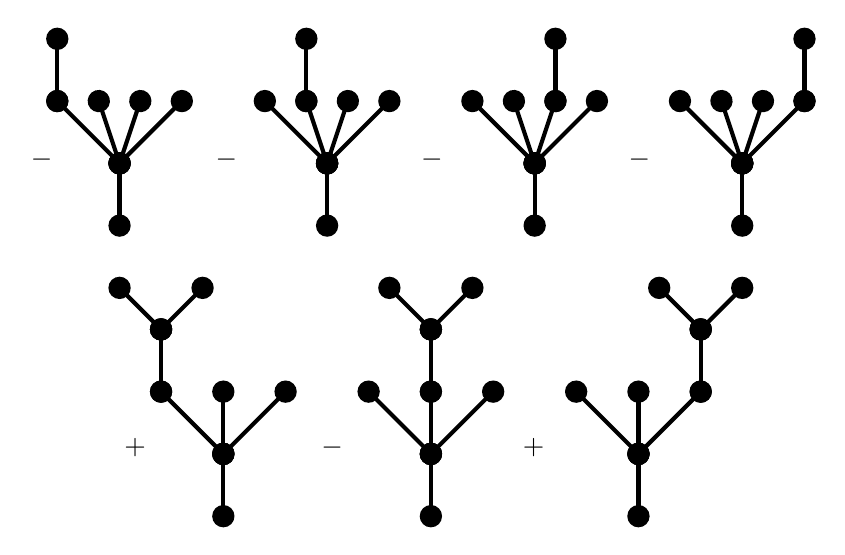
\begin{tikzpicture}[x=0.75pt,y=0.75pt,yscale=-1,xscale=1]
%uncomment if require: \path (0,300); %set diagram left start at 0, and has height of 300

%Straight Lines [id:da7271236022900844] 
\draw [line width=1.5]    (50,70) -- (20,40) ;
\draw [shift={(20,40)}, rotate = 225] [color={rgb, 255:red, 0; green, 0; blue, 0 }  ][fill={rgb, 255:red, 0; green, 0; blue, 0 }  ][line width=1.5]      (0, 0) circle [x radius= 4.36, y radius= 4.36]   ;
\draw [shift={(50,70)}, rotate = 225] [color={rgb, 255:red, 0; green, 0; blue, 0 }  ][fill={rgb, 255:red, 0; green, 0; blue, 0 }  ][line width=1.5]      (0, 0) circle [x radius= 4.36, y radius= 4.36]   ;
%Straight Lines [id:da8829298962249057] 
\draw [line width=1.5]    (50,70) -- (40,40) ;
\draw [shift={(40,40)}, rotate = 251.57] [color={rgb, 255:red, 0; green, 0; blue, 0 }  ][fill={rgb, 255:red, 0; green, 0; blue, 0 }  ][line width=1.5]      (0, 0) circle [x radius= 4.36, y radius= 4.36]   ;
\draw [shift={(50,70)}, rotate = 251.57] [color={rgb, 255:red, 0; green, 0; blue, 0 }  ][fill={rgb, 255:red, 0; green, 0; blue, 0 }  ][line width=1.5]      (0, 0) circle [x radius= 4.36, y radius= 4.36]   ;
%Straight Lines [id:da14019661944022443] 
\draw [line width=1.5]    (50,70) -- (80,40) ;
\draw [shift={(80,40)}, rotate = 315] [color={rgb, 255:red, 0; green, 0; blue, 0 }  ][fill={rgb, 255:red, 0; green, 0; blue, 0 }  ][line width=1.5]      (0, 0) circle [x radius= 4.36, y radius= 4.36]   ;
\draw [shift={(50,70)}, rotate = 315] [color={rgb, 255:red, 0; green, 0; blue, 0 }  ][fill={rgb, 255:red, 0; green, 0; blue, 0 }  ][line width=1.5]      (0, 0) circle [x radius= 4.36, y radius= 4.36]   ;
%Straight Lines [id:da3561053996918748] 
\draw [line width=1.5]    (50,100) -- (50,70) ;
\draw [shift={(50,70)}, rotate = 270] [color={rgb, 255:red, 0; green, 0; blue, 0 }  ][fill={rgb, 255:red, 0; green, 0; blue, 0 }  ][line width=1.5]      (0, 0) circle [x radius= 4.36, y radius= 4.36]   ;
\draw [shift={(50,100)}, rotate = 270] [color={rgb, 255:red, 0; green, 0; blue, 0 }  ][fill={rgb, 255:red, 0; green, 0; blue, 0 }  ][line width=1.5]      (0, 0) circle [x radius= 4.36, y radius= 4.36]   ;
%Straight Lines [id:da12959305658190345] 
\draw [line width=1.5]    (60,40) -- (50,70) ;
\draw [shift={(50,70)}, rotate = 108.43] [color={rgb, 255:red, 0; green, 0; blue, 0 }  ][fill={rgb, 255:red, 0; green, 0; blue, 0 }  ][line width=1.5]      (0, 0) circle [x radius= 4.36, y radius= 4.36]   ;
\draw [shift={(60,40)}, rotate = 108.43] [color={rgb, 255:red, 0; green, 0; blue, 0 }  ][fill={rgb, 255:red, 0; green, 0; blue, 0 }  ][line width=1.5]      (0, 0) circle [x radius= 4.36, y radius= 4.36]   ;
%Straight Lines [id:da17788889705056876] 
\draw [line width=1.5]    (150,70) -- (120,40) ;
\draw [shift={(120,40)}, rotate = 225] [color={rgb, 255:red, 0; green, 0; blue, 0 }  ][fill={rgb, 255:red, 0; green, 0; blue, 0 }  ][line width=1.5]      (0, 0) circle [x radius= 4.36, y radius= 4.36]   ;
\draw [shift={(150,70)}, rotate = 225] [color={rgb, 255:red, 0; green, 0; blue, 0 }  ][fill={rgb, 255:red, 0; green, 0; blue, 0 }  ][line width=1.5]      (0, 0) circle [x radius= 4.36, y radius= 4.36]   ;
%Straight Lines [id:da32726690992182617] 
\draw [line width=1.5]    (150,70) -- (140,40) ;
\draw [shift={(140,40)}, rotate = 251.57] [color={rgb, 255:red, 0; green, 0; blue, 0 }  ][fill={rgb, 255:red, 0; green, 0; blue, 0 }  ][line width=1.5]      (0, 0) circle [x radius= 4.36, y radius= 4.36]   ;
\draw [shift={(150,70)}, rotate = 251.57] [color={rgb, 255:red, 0; green, 0; blue, 0 }  ][fill={rgb, 255:red, 0; green, 0; blue, 0 }  ][line width=1.5]      (0, 0) circle [x radius= 4.36, y radius= 4.36]   ;
%Straight Lines [id:da6529521762459134] 
\draw [line width=1.5]    (150,70) -- (180,40) ;
\draw [shift={(180,40)}, rotate = 315] [color={rgb, 255:red, 0; green, 0; blue, 0 }  ][fill={rgb, 255:red, 0; green, 0; blue, 0 }  ][line width=1.5]      (0, 0) circle [x radius= 4.36, y radius= 4.36]   ;
\draw [shift={(150,70)}, rotate = 315] [color={rgb, 255:red, 0; green, 0; blue, 0 }  ][fill={rgb, 255:red, 0; green, 0; blue, 0 }  ][line width=1.5]      (0, 0) circle [x radius= 4.36, y radius= 4.36]   ;
%Straight Lines [id:da10508941767197344] 
\draw [line width=1.5]    (150,100) -- (150,70) ;
\draw [shift={(150,70)}, rotate = 270] [color={rgb, 255:red, 0; green, 0; blue, 0 }  ][fill={rgb, 255:red, 0; green, 0; blue, 0 }  ][line width=1.5]      (0, 0) circle [x radius= 4.36, y radius= 4.36]   ;
\draw [shift={(150,100)}, rotate = 270] [color={rgb, 255:red, 0; green, 0; blue, 0 }  ][fill={rgb, 255:red, 0; green, 0; blue, 0 }  ][line width=1.5]      (0, 0) circle [x radius= 4.36, y radius= 4.36]   ;
%Straight Lines [id:da6259633442377939] 
\draw [line width=1.5]    (160,40) -- (150,70) ;
\draw [shift={(150,70)}, rotate = 108.43] [color={rgb, 255:red, 0; green, 0; blue, 0 }  ][fill={rgb, 255:red, 0; green, 0; blue, 0 }  ][line width=1.5]      (0, 0) circle [x radius= 4.36, y radius= 4.36]   ;
\draw [shift={(160,40)}, rotate = 108.43] [color={rgb, 255:red, 0; green, 0; blue, 0 }  ][fill={rgb, 255:red, 0; green, 0; blue, 0 }  ][line width=1.5]      (0, 0) circle [x radius= 4.36, y radius= 4.36]   ;
%Straight Lines [id:da18827403823128308] 
\draw [line width=1.5]    (250,70) -- (220,40) ;
\draw [shift={(220,40)}, rotate = 225] [color={rgb, 255:red, 0; green, 0; blue, 0 }  ][fill={rgb, 255:red, 0; green, 0; blue, 0 }  ][line width=1.5]      (0, 0) circle [x radius= 4.36, y radius= 4.36]   ;
\draw [shift={(250,70)}, rotate = 225] [color={rgb, 255:red, 0; green, 0; blue, 0 }  ][fill={rgb, 255:red, 0; green, 0; blue, 0 }  ][line width=1.5]      (0, 0) circle [x radius= 4.36, y radius= 4.36]   ;
%Straight Lines [id:da4416224263321782] 
\draw [line width=1.5]    (250,70) -- (240,40) ;
\draw [shift={(240,40)}, rotate = 251.57] [color={rgb, 255:red, 0; green, 0; blue, 0 }  ][fill={rgb, 255:red, 0; green, 0; blue, 0 }  ][line width=1.5]      (0, 0) circle [x radius= 4.36, y radius= 4.36]   ;
\draw [shift={(250,70)}, rotate = 251.57] [color={rgb, 255:red, 0; green, 0; blue, 0 }  ][fill={rgb, 255:red, 0; green, 0; blue, 0 }  ][line width=1.5]      (0, 0) circle [x radius= 4.36, y radius= 4.36]   ;
%Straight Lines [id:da4912193105487581] 
\draw [line width=1.5]    (250,70) -- (280,40) ;
\draw [shift={(280,40)}, rotate = 315] [color={rgb, 255:red, 0; green, 0; blue, 0 }  ][fill={rgb, 255:red, 0; green, 0; blue, 0 }  ][line width=1.5]      (0, 0) circle [x radius= 4.36, y radius= 4.36]   ;
\draw [shift={(250,70)}, rotate = 315] [color={rgb, 255:red, 0; green, 0; blue, 0 }  ][fill={rgb, 255:red, 0; green, 0; blue, 0 }  ][line width=1.5]      (0, 0) circle [x radius= 4.36, y radius= 4.36]   ;
%Straight Lines [id:da057140828311111225] 
\draw [line width=1.5]    (250,100) -- (250,70) ;
\draw [shift={(250,70)}, rotate = 270] [color={rgb, 255:red, 0; green, 0; blue, 0 }  ][fill={rgb, 255:red, 0; green, 0; blue, 0 }  ][line width=1.5]      (0, 0) circle [x radius= 4.36, y radius= 4.36]   ;
\draw [shift={(250,100)}, rotate = 270] [color={rgb, 255:red, 0; green, 0; blue, 0 }  ][fill={rgb, 255:red, 0; green, 0; blue, 0 }  ][line width=1.5]      (0, 0) circle [x radius= 4.36, y radius= 4.36]   ;
%Straight Lines [id:da6532175337656438] 
\draw [line width=1.5]    (260,40) -- (250,70) ;
\draw [shift={(250,70)}, rotate = 108.43] [color={rgb, 255:red, 0; green, 0; blue, 0 }  ][fill={rgb, 255:red, 0; green, 0; blue, 0 }  ][line width=1.5]      (0, 0) circle [x radius= 4.36, y radius= 4.36]   ;
\draw [shift={(260,40)}, rotate = 108.43] [color={rgb, 255:red, 0; green, 0; blue, 0 }  ][fill={rgb, 255:red, 0; green, 0; blue, 0 }  ][line width=1.5]      (0, 0) circle [x radius= 4.36, y radius= 4.36]   ;
%Straight Lines [id:da9439423309856876] 
\draw [line width=1.5]    (350,70) -- (320,40) ;
\draw [shift={(320,40)}, rotate = 225] [color={rgb, 255:red, 0; green, 0; blue, 0 }  ][fill={rgb, 255:red, 0; green, 0; blue, 0 }  ][line width=1.5]      (0, 0) circle [x radius= 4.36, y radius= 4.36]   ;
\draw [shift={(350,70)}, rotate = 225] [color={rgb, 255:red, 0; green, 0; blue, 0 }  ][fill={rgb, 255:red, 0; green, 0; blue, 0 }  ][line width=1.5]      (0, 0) circle [x radius= 4.36, y radius= 4.36]   ;
%Straight Lines [id:da6793777254659024] 
\draw [line width=1.5]    (350,70) -- (340,40) ;
\draw [shift={(340,40)}, rotate = 251.57] [color={rgb, 255:red, 0; green, 0; blue, 0 }  ][fill={rgb, 255:red, 0; green, 0; blue, 0 }  ][line width=1.5]      (0, 0) circle [x radius= 4.36, y radius= 4.36]   ;
\draw [shift={(350,70)}, rotate = 251.57] [color={rgb, 255:red, 0; green, 0; blue, 0 }  ][fill={rgb, 255:red, 0; green, 0; blue, 0 }  ][line width=1.5]      (0, 0) circle [x radius= 4.36, y radius= 4.36]   ;
%Straight Lines [id:da4673813785992058] 
\draw [line width=1.5]    (350,70) -- (380,40) ;
\draw [shift={(380,40)}, rotate = 315] [color={rgb, 255:red, 0; green, 0; blue, 0 }  ][fill={rgb, 255:red, 0; green, 0; blue, 0 }  ][line width=1.5]      (0, 0) circle [x radius= 4.36, y radius= 4.36]   ;
\draw [shift={(350,70)}, rotate = 315] [color={rgb, 255:red, 0; green, 0; blue, 0 }  ][fill={rgb, 255:red, 0; green, 0; blue, 0 }  ][line width=1.5]      (0, 0) circle [x radius= 4.36, y radius= 4.36]   ;
%Straight Lines [id:da2972746595471605] 
\draw [line width=1.5]    (350,100) -- (350,70) ;
\draw [shift={(350,70)}, rotate = 270] [color={rgb, 255:red, 0; green, 0; blue, 0 }  ][fill={rgb, 255:red, 0; green, 0; blue, 0 }  ][line width=1.5]      (0, 0) circle [x radius= 4.36, y radius= 4.36]   ;
\draw [shift={(350,100)}, rotate = 270] [color={rgb, 255:red, 0; green, 0; blue, 0 }  ][fill={rgb, 255:red, 0; green, 0; blue, 0 }  ][line width=1.5]      (0, 0) circle [x radius= 4.36, y radius= 4.36]   ;
%Straight Lines [id:da526738135792] 
\draw [line width=1.5]    (360,40) -- (350,70) ;
\draw [shift={(350,70)}, rotate = 108.43] [color={rgb, 255:red, 0; green, 0; blue, 0 }  ][fill={rgb, 255:red, 0; green, 0; blue, 0 }  ][line width=1.5]      (0, 0) circle [x radius= 4.36, y radius= 4.36]   ;
\draw [shift={(360,40)}, rotate = 108.43] [color={rgb, 255:red, 0; green, 0; blue, 0 }  ][fill={rgb, 255:red, 0; green, 0; blue, 0 }  ][line width=1.5]      (0, 0) circle [x radius= 4.36, y radius= 4.36]   ;
%Straight Lines [id:da3439286430792807] 
\draw [line width=1.5]    (20,40) -- (20,10) ;
\draw [shift={(20,10)}, rotate = 270] [color={rgb, 255:red, 0; green, 0; blue, 0 }  ][fill={rgb, 255:red, 0; green, 0; blue, 0 }  ][line width=1.5]      (0, 0) circle [x radius= 4.36, y radius= 4.36]   ;
\draw [shift={(20,40)}, rotate = 270] [color={rgb, 255:red, 0; green, 0; blue, 0 }  ][fill={rgb, 255:red, 0; green, 0; blue, 0 }  ][line width=1.5]      (0, 0) circle [x radius= 4.36, y radius= 4.36]   ;
%Straight Lines [id:da027749002350105467] 
\draw [line width=1.5]    (140,40) -- (140,10) ;
\draw [shift={(140,10)}, rotate = 270] [color={rgb, 255:red, 0; green, 0; blue, 0 }  ][fill={rgb, 255:red, 0; green, 0; blue, 0 }  ][line width=1.5]      (0, 0) circle [x radius= 4.36, y radius= 4.36]   ;
\draw [shift={(140,40)}, rotate = 270] [color={rgb, 255:red, 0; green, 0; blue, 0 }  ][fill={rgb, 255:red, 0; green, 0; blue, 0 }  ][line width=1.5]      (0, 0) circle [x radius= 4.36, y radius= 4.36]   ;
%Straight Lines [id:da4141601555763963] 
\draw [line width=1.5]    (260,40) -- (260,10) ;
\draw [shift={(260,10)}, rotate = 270] [color={rgb, 255:red, 0; green, 0; blue, 0 }  ][fill={rgb, 255:red, 0; green, 0; blue, 0 }  ][line width=1.5]      (0, 0) circle [x radius= 4.36, y radius= 4.36]   ;
\draw [shift={(260,40)}, rotate = 270] [color={rgb, 255:red, 0; green, 0; blue, 0 }  ][fill={rgb, 255:red, 0; green, 0; blue, 0 }  ][line width=1.5]      (0, 0) circle [x radius= 4.36, y radius= 4.36]   ;
%Straight Lines [id:da8143971343614638] 
\draw [line width=1.5]    (380,40) -- (380,10) ;
\draw [shift={(380,10)}, rotate = 270] [color={rgb, 255:red, 0; green, 0; blue, 0 }  ][fill={rgb, 255:red, 0; green, 0; blue, 0 }  ][line width=1.5]      (0, 0) circle [x radius= 4.36, y radius= 4.36]   ;
\draw [shift={(380,40)}, rotate = 270] [color={rgb, 255:red, 0; green, 0; blue, 0 }  ][fill={rgb, 255:red, 0; green, 0; blue, 0 }  ][line width=1.5]      (0, 0) circle [x radius= 4.36, y radius= 4.36]   ;
%Straight Lines [id:da5027840919946027] 
\draw [line width=1.5]    (100,210) -- (70,180) ;
\draw [shift={(70,180)}, rotate = 225] [color={rgb, 255:red, 0; green, 0; blue, 0 }  ][fill={rgb, 255:red, 0; green, 0; blue, 0 }  ][line width=1.5]      (0, 0) circle [x radius= 4.36, y radius= 4.36]   ;
\draw [shift={(100,210)}, rotate = 225] [color={rgb, 255:red, 0; green, 0; blue, 0 }  ][fill={rgb, 255:red, 0; green, 0; blue, 0 }  ][line width=1.5]      (0, 0) circle [x radius= 4.36, y radius= 4.36]   ;
%Straight Lines [id:da012169408330350517] 
\draw [line width=1.5]    (100,210) -- (100,180) ;
\draw [shift={(100,180)}, rotate = 270] [color={rgb, 255:red, 0; green, 0; blue, 0 }  ][fill={rgb, 255:red, 0; green, 0; blue, 0 }  ][line width=1.5]      (0, 0) circle [x radius= 4.36, y radius= 4.36]   ;
\draw [shift={(100,210)}, rotate = 270] [color={rgb, 255:red, 0; green, 0; blue, 0 }  ][fill={rgb, 255:red, 0; green, 0; blue, 0 }  ][line width=1.5]      (0, 0) circle [x radius= 4.36, y radius= 4.36]   ;
%Straight Lines [id:da3794956070144304] 
\draw [line width=1.5]    (100,210) -- (130,180) ;
\draw [shift={(130,180)}, rotate = 315] [color={rgb, 255:red, 0; green, 0; blue, 0 }  ][fill={rgb, 255:red, 0; green, 0; blue, 0 }  ][line width=1.5]      (0, 0) circle [x radius= 4.36, y radius= 4.36]   ;
\draw [shift={(100,210)}, rotate = 315] [color={rgb, 255:red, 0; green, 0; blue, 0 }  ][fill={rgb, 255:red, 0; green, 0; blue, 0 }  ][line width=1.5]      (0, 0) circle [x radius= 4.36, y radius= 4.36]   ;
%Straight Lines [id:da8996197602070666] 
\draw [line width=1.5]    (100,240) -- (100,210) ;
\draw [shift={(100,210)}, rotate = 270] [color={rgb, 255:red, 0; green, 0; blue, 0 }  ][fill={rgb, 255:red, 0; green, 0; blue, 0 }  ][line width=1.5]      (0, 0) circle [x radius= 4.36, y radius= 4.36]   ;
\draw [shift={(100,240)}, rotate = 270] [color={rgb, 255:red, 0; green, 0; blue, 0 }  ][fill={rgb, 255:red, 0; green, 0; blue, 0 }  ][line width=1.5]      (0, 0) circle [x radius= 4.36, y radius= 4.36]   ;
%Straight Lines [id:da1531842966441921] 
\draw [line width=1.5]    (70,150) -- (50,130) ;
\draw [shift={(50,130)}, rotate = 225] [color={rgb, 255:red, 0; green, 0; blue, 0 }  ][fill={rgb, 255:red, 0; green, 0; blue, 0 }  ][line width=1.5]      (0, 0) circle [x radius= 4.36, y radius= 4.36]   ;
\draw [shift={(70,150)}, rotate = 225] [color={rgb, 255:red, 0; green, 0; blue, 0 }  ][fill={rgb, 255:red, 0; green, 0; blue, 0 }  ][line width=1.5]      (0, 0) circle [x radius= 4.36, y radius= 4.36]   ;
%Straight Lines [id:da5635603151723407] 
\draw [line width=1.5]    (70,150) -- (90,130) ;
\draw [shift={(90,130)}, rotate = 315] [color={rgb, 255:red, 0; green, 0; blue, 0 }  ][fill={rgb, 255:red, 0; green, 0; blue, 0 }  ][line width=1.5]      (0, 0) circle [x radius= 4.36, y radius= 4.36]   ;
\draw [shift={(70,150)}, rotate = 315] [color={rgb, 255:red, 0; green, 0; blue, 0 }  ][fill={rgb, 255:red, 0; green, 0; blue, 0 }  ][line width=1.5]      (0, 0) circle [x radius= 4.36, y radius= 4.36]   ;
%Straight Lines [id:da37599967010410107] 
\draw [line width=1.5]    (70,180) -- (70,150) ;
\draw [shift={(70,150)}, rotate = 270] [color={rgb, 255:red, 0; green, 0; blue, 0 }  ][fill={rgb, 255:red, 0; green, 0; blue, 0 }  ][line width=1.5]      (0, 0) circle [x radius= 4.36, y radius= 4.36]   ;
\draw [shift={(70,180)}, rotate = 270] [color={rgb, 255:red, 0; green, 0; blue, 0 }  ][fill={rgb, 255:red, 0; green, 0; blue, 0 }  ][line width=1.5]      (0, 0) circle [x radius= 4.36, y radius= 4.36]   ;
%Straight Lines [id:da698265177656928] 
\draw [line width=1.5]    (200,210) -- (170,180) ;
\draw [shift={(170,180)}, rotate = 225] [color={rgb, 255:red, 0; green, 0; blue, 0 }  ][fill={rgb, 255:red, 0; green, 0; blue, 0 }  ][line width=1.5]      (0, 0) circle [x radius= 4.36, y radius= 4.36]   ;
\draw [shift={(200,210)}, rotate = 225] [color={rgb, 255:red, 0; green, 0; blue, 0 }  ][fill={rgb, 255:red, 0; green, 0; blue, 0 }  ][line width=1.5]      (0, 0) circle [x radius= 4.36, y radius= 4.36]   ;
%Straight Lines [id:da049456703112388256] 
\draw [line width=1.5]    (200,210) -- (200,180) ;
\draw [shift={(200,180)}, rotate = 270] [color={rgb, 255:red, 0; green, 0; blue, 0 }  ][fill={rgb, 255:red, 0; green, 0; blue, 0 }  ][line width=1.5]      (0, 0) circle [x radius= 4.36, y radius= 4.36]   ;
\draw [shift={(200,210)}, rotate = 270] [color={rgb, 255:red, 0; green, 0; blue, 0 }  ][fill={rgb, 255:red, 0; green, 0; blue, 0 }  ][line width=1.5]      (0, 0) circle [x radius= 4.36, y radius= 4.36]   ;
%Straight Lines [id:da19781405329398405] 
\draw [line width=1.5]    (200,210) -- (230,180) ;
\draw [shift={(230,180)}, rotate = 315] [color={rgb, 255:red, 0; green, 0; blue, 0 }  ][fill={rgb, 255:red, 0; green, 0; blue, 0 }  ][line width=1.5]      (0, 0) circle [x radius= 4.36, y radius= 4.36]   ;
\draw [shift={(200,210)}, rotate = 315] [color={rgb, 255:red, 0; green, 0; blue, 0 }  ][fill={rgb, 255:red, 0; green, 0; blue, 0 }  ][line width=1.5]      (0, 0) circle [x radius= 4.36, y radius= 4.36]   ;
%Straight Lines [id:da9771660287757578] 
\draw [line width=1.5]    (200,240) -- (200,210) ;
\draw [shift={(200,210)}, rotate = 270] [color={rgb, 255:red, 0; green, 0; blue, 0 }  ][fill={rgb, 255:red, 0; green, 0; blue, 0 }  ][line width=1.5]      (0, 0) circle [x radius= 4.36, y radius= 4.36]   ;
\draw [shift={(200,240)}, rotate = 270] [color={rgb, 255:red, 0; green, 0; blue, 0 }  ][fill={rgb, 255:red, 0; green, 0; blue, 0 }  ][line width=1.5]      (0, 0) circle [x radius= 4.36, y radius= 4.36]   ;
%Straight Lines [id:da8050669462477833] 
\draw [line width=1.5]    (200,150) -- (180,130) ;
\draw [shift={(180,130)}, rotate = 225] [color={rgb, 255:red, 0; green, 0; blue, 0 }  ][fill={rgb, 255:red, 0; green, 0; blue, 0 }  ][line width=1.5]      (0, 0) circle [x radius= 4.36, y radius= 4.36]   ;
\draw [shift={(200,150)}, rotate = 225] [color={rgb, 255:red, 0; green, 0; blue, 0 }  ][fill={rgb, 255:red, 0; green, 0; blue, 0 }  ][line width=1.5]      (0, 0) circle [x radius= 4.36, y radius= 4.36]   ;
%Straight Lines [id:da4433467710630703] 
\draw [line width=1.5]    (200,150) -- (220,130) ;
\draw [shift={(220,130)}, rotate = 315] [color={rgb, 255:red, 0; green, 0; blue, 0 }  ][fill={rgb, 255:red, 0; green, 0; blue, 0 }  ][line width=1.5]      (0, 0) circle [x radius= 4.36, y radius= 4.36]   ;
\draw [shift={(200,150)}, rotate = 315] [color={rgb, 255:red, 0; green, 0; blue, 0 }  ][fill={rgb, 255:red, 0; green, 0; blue, 0 }  ][line width=1.5]      (0, 0) circle [x radius= 4.36, y radius= 4.36]   ;
%Straight Lines [id:da01581391478939298] 
\draw [line width=1.5]    (200,180) -- (200,150) ;
\draw [shift={(200,150)}, rotate = 270] [color={rgb, 255:red, 0; green, 0; blue, 0 }  ][fill={rgb, 255:red, 0; green, 0; blue, 0 }  ][line width=1.5]      (0, 0) circle [x radius= 4.36, y radius= 4.36]   ;
\draw [shift={(200,180)}, rotate = 270] [color={rgb, 255:red, 0; green, 0; blue, 0 }  ][fill={rgb, 255:red, 0; green, 0; blue, 0 }  ][line width=1.5]      (0, 0) circle [x radius= 4.36, y radius= 4.36]   ;
%Straight Lines [id:da39290163971213876] 
\draw [line width=1.5]    (300,210) -- (270,180) ;
\draw [shift={(270,180)}, rotate = 225] [color={rgb, 255:red, 0; green, 0; blue, 0 }  ][fill={rgb, 255:red, 0; green, 0; blue, 0 }  ][line width=1.5]      (0, 0) circle [x radius= 4.36, y radius= 4.36]   ;
\draw [shift={(300,210)}, rotate = 225] [color={rgb, 255:red, 0; green, 0; blue, 0 }  ][fill={rgb, 255:red, 0; green, 0; blue, 0 }  ][line width=1.5]      (0, 0) circle [x radius= 4.36, y radius= 4.36]   ;
%Straight Lines [id:da6585976068778385] 
\draw [line width=1.5]    (300,210) -- (300,180) ;
\draw [shift={(300,180)}, rotate = 270] [color={rgb, 255:red, 0; green, 0; blue, 0 }  ][fill={rgb, 255:red, 0; green, 0; blue, 0 }  ][line width=1.5]      (0, 0) circle [x radius= 4.36, y radius= 4.36]   ;
\draw [shift={(300,210)}, rotate = 270] [color={rgb, 255:red, 0; green, 0; blue, 0 }  ][fill={rgb, 255:red, 0; green, 0; blue, 0 }  ][line width=1.5]      (0, 0) circle [x radius= 4.36, y radius= 4.36]   ;
%Straight Lines [id:da08497570166304391] 
\draw [line width=1.5]    (300,210) -- (330,180) ;
\draw [shift={(330,180)}, rotate = 315] [color={rgb, 255:red, 0; green, 0; blue, 0 }  ][fill={rgb, 255:red, 0; green, 0; blue, 0 }  ][line width=1.5]      (0, 0) circle [x radius= 4.36, y radius= 4.36]   ;
\draw [shift={(300,210)}, rotate = 315] [color={rgb, 255:red, 0; green, 0; blue, 0 }  ][fill={rgb, 255:red, 0; green, 0; blue, 0 }  ][line width=1.5]      (0, 0) circle [x radius= 4.36, y radius= 4.36]   ;
%Straight Lines [id:da6049966997095673] 
\draw [line width=1.5]    (300,240) -- (300,210) ;
\draw [shift={(300,210)}, rotate = 270] [color={rgb, 255:red, 0; green, 0; blue, 0 }  ][fill={rgb, 255:red, 0; green, 0; blue, 0 }  ][line width=1.5]      (0, 0) circle [x radius= 4.36, y radius= 4.36]   ;
\draw [shift={(300,240)}, rotate = 270] [color={rgb, 255:red, 0; green, 0; blue, 0 }  ][fill={rgb, 255:red, 0; green, 0; blue, 0 }  ][line width=1.5]      (0, 0) circle [x radius= 4.36, y radius= 4.36]   ;
%Straight Lines [id:da3027007292774597] 
\draw [line width=1.5]    (330,150) -- (310,130) ;
\draw [shift={(310,130)}, rotate = 225] [color={rgb, 255:red, 0; green, 0; blue, 0 }  ][fill={rgb, 255:red, 0; green, 0; blue, 0 }  ][line width=1.5]      (0, 0) circle [x radius= 4.36, y radius= 4.36]   ;
\draw [shift={(330,150)}, rotate = 225] [color={rgb, 255:red, 0; green, 0; blue, 0 }  ][fill={rgb, 255:red, 0; green, 0; blue, 0 }  ][line width=1.5]      (0, 0) circle [x radius= 4.36, y radius= 4.36]   ;
%Straight Lines [id:da8425409794662362] 
\draw [line width=1.5]    (330,150) -- (350,130) ;
\draw [shift={(350,130)}, rotate = 315] [color={rgb, 255:red, 0; green, 0; blue, 0 }  ][fill={rgb, 255:red, 0; green, 0; blue, 0 }  ][line width=1.5]      (0, 0) circle [x radius= 4.36, y radius= 4.36]   ;
\draw [shift={(330,150)}, rotate = 315] [color={rgb, 255:red, 0; green, 0; blue, 0 }  ][fill={rgb, 255:red, 0; green, 0; blue, 0 }  ][line width=1.5]      (0, 0) circle [x radius= 4.36, y radius= 4.36]   ;
%Straight Lines [id:da6597509617717114] 
\draw [line width=1.5]    (330,180) -- (330,150) ;
\draw [shift={(330,150)}, rotate = 270] [color={rgb, 255:red, 0; green, 0; blue, 0 }  ][fill={rgb, 255:red, 0; green, 0; blue, 0 }  ][line width=1.5]      (0, 0) circle [x radius= 4.36, y radius= 4.36]   ;
\draw [shift={(330,180)}, rotate = 270] [color={rgb, 255:red, 0; green, 0; blue, 0 }  ][fill={rgb, 255:red, 0; green, 0; blue, 0 }  ][line width=1.5]      (0, 0) circle [x radius= 4.36, y radius= 4.36]   ;

% Text Node
\draw (6,62.4) node [anchor=north west][inner sep=0.75pt]    {$-$};
% Text Node
\draw (95,62.4) node [anchor=north west][inner sep=0.75pt]    {$-$};
% Text Node
\draw (194,62.4) node [anchor=north west][inner sep=0.75pt]    {$-$};
% Text Node
\draw (294,62.4) node [anchor=north west][inner sep=0.75pt]    {$-$};
% Text Node
\draw (146,201.4) node [anchor=north west][inner sep=0.75pt]    {$-$};
% Text Node
\draw (51,201.4) node [anchor=north west][inner sep=0.75pt]    {$+$};
% Text Node
\draw (243,201.4) node [anchor=north west][inner sep=0.75pt]    {$+$};


\end{tikzpicture}   
\end{center}

\begin{enumerate}
\setcounter{enumi}{6}
    \item We continue this process downward, and draw $n-2$ copies of $m_{n-2}$, and put a copy of $m_3$ at each leaf. The signs are again all negative or all positive, depending on weather $n$ is even or odd. The dependence is the same as for the first one. 
\end{enumerate}

The general process for drawing the $i$'th step is drawing $n-i$ copies of the rooted tree that represent $m_{n-i}$. Then put a copy of the rooted tree that represents $m_{i+1}$ on each of of the leaves in succession from left to right, never more than one per copy. If $i+1=n$ then we have a single tree $m_1 m_{n}$, which gets a positive sign. If $n$ is odd and $i$ is even, then put negative signs in front of all of them. If $n$ and $i$ are both even, then put a positive sign in front of all of them. Finally, if $i$ is odd, put alternating signs, starting at positive, in front of them. When we have done this process for all $i$, where $0\leq i \leq n$, then we have an upside down triangle. When we sum up all the different layers, we get $0$. 

For our $n=4$ example the final triangle would look like

% The complete Stasheff identity for n=4, with signs



\begin{center}
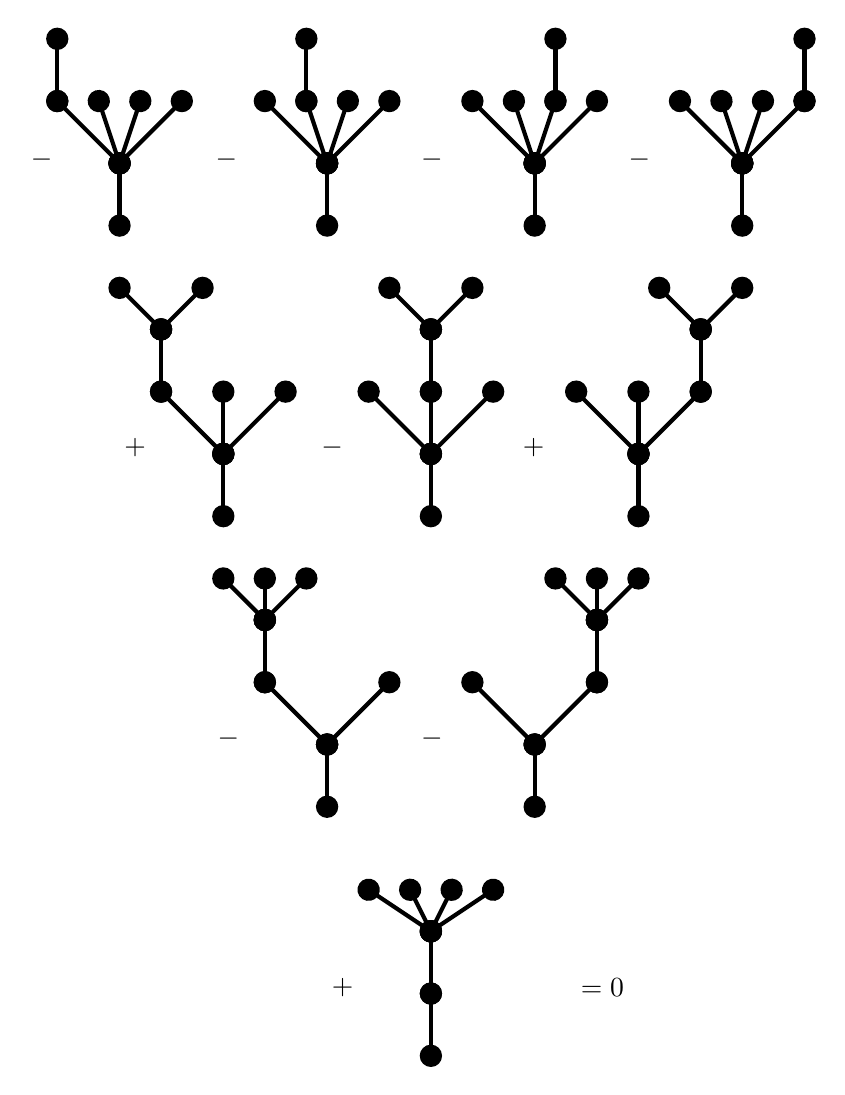
\begin{tikzpicture}[x=0.75pt,y=0.75pt,yscale=-1,xscale=1]
%uncomment if require: \path (0,513); %set diagram left start at 0, and has height of 513

%Straight Lines [id:da7271236022900844] 
\draw [line width=1.5]    (50,70) -- (20,40) ;
\draw [shift={(20,40)}, rotate = 225] [color={rgb, 255:red, 0; green, 0; blue, 0 }  ][fill={rgb, 255:red, 0; green, 0; blue, 0 }  ][line width=1.5]      (0, 0) circle [x radius= 4.36, y radius= 4.36]   ;
\draw [shift={(50,70)}, rotate = 225] [color={rgb, 255:red, 0; green, 0; blue, 0 }  ][fill={rgb, 255:red, 0; green, 0; blue, 0 }  ][line width=1.5]      (0, 0) circle [x radius= 4.36, y radius= 4.36]   ;
%Straight Lines [id:da8829298962249057] 
\draw [line width=1.5]    (50,70) -- (40,40) ;
\draw [shift={(40,40)}, rotate = 251.57] [color={rgb, 255:red, 0; green, 0; blue, 0 }  ][fill={rgb, 255:red, 0; green, 0; blue, 0 }  ][line width=1.5]      (0, 0) circle [x radius= 4.36, y radius= 4.36]   ;
\draw [shift={(50,70)}, rotate = 251.57] [color={rgb, 255:red, 0; green, 0; blue, 0 }  ][fill={rgb, 255:red, 0; green, 0; blue, 0 }  ][line width=1.5]      (0, 0) circle [x radius= 4.36, y radius= 4.36]   ;
%Straight Lines [id:da14019661944022443] 
\draw [line width=1.5]    (50,70) -- (80,40) ;
\draw [shift={(80,40)}, rotate = 315] [color={rgb, 255:red, 0; green, 0; blue, 0 }  ][fill={rgb, 255:red, 0; green, 0; blue, 0 }  ][line width=1.5]      (0, 0) circle [x radius= 4.36, y radius= 4.36]   ;
\draw [shift={(50,70)}, rotate = 315] [color={rgb, 255:red, 0; green, 0; blue, 0 }  ][fill={rgb, 255:red, 0; green, 0; blue, 0 }  ][line width=1.5]      (0, 0) circle [x radius= 4.36, y radius= 4.36]   ;
%Straight Lines [id:da3561053996918748] 
\draw [line width=1.5]    (50,100) -- (50,70) ;
\draw [shift={(50,70)}, rotate = 270] [color={rgb, 255:red, 0; green, 0; blue, 0 }  ][fill={rgb, 255:red, 0; green, 0; blue, 0 }  ][line width=1.5]      (0, 0) circle [x radius= 4.36, y radius= 4.36]   ;
\draw [shift={(50,100)}, rotate = 270] [color={rgb, 255:red, 0; green, 0; blue, 0 }  ][fill={rgb, 255:red, 0; green, 0; blue, 0 }  ][line width=1.5]      (0, 0) circle [x radius= 4.36, y radius= 4.36]   ;
%Straight Lines [id:da12959305658190345] 
\draw [line width=1.5]    (60,40) -- (50,70) ;
\draw [shift={(50,70)}, rotate = 108.43] [color={rgb, 255:red, 0; green, 0; blue, 0 }  ][fill={rgb, 255:red, 0; green, 0; blue, 0 }  ][line width=1.5]      (0, 0) circle [x radius= 4.36, y radius= 4.36]   ;
\draw [shift={(60,40)}, rotate = 108.43] [color={rgb, 255:red, 0; green, 0; blue, 0 }  ][fill={rgb, 255:red, 0; green, 0; blue, 0 }  ][line width=1.5]      (0, 0) circle [x radius= 4.36, y radius= 4.36]   ;
%Straight Lines [id:da17788889705056876] 
\draw [line width=1.5]    (150,70) -- (120,40) ;
\draw [shift={(120,40)}, rotate = 225] [color={rgb, 255:red, 0; green, 0; blue, 0 }  ][fill={rgb, 255:red, 0; green, 0; blue, 0 }  ][line width=1.5]      (0, 0) circle [x radius= 4.36, y radius= 4.36]   ;
\draw [shift={(150,70)}, rotate = 225] [color={rgb, 255:red, 0; green, 0; blue, 0 }  ][fill={rgb, 255:red, 0; green, 0; blue, 0 }  ][line width=1.5]      (0, 0) circle [x radius= 4.36, y radius= 4.36]   ;
%Straight Lines [id:da32726690992182617] 
\draw [line width=1.5]    (150,70) -- (140,40) ;
\draw [shift={(140,40)}, rotate = 251.57] [color={rgb, 255:red, 0; green, 0; blue, 0 }  ][fill={rgb, 255:red, 0; green, 0; blue, 0 }  ][line width=1.5]      (0, 0) circle [x radius= 4.36, y radius= 4.36]   ;
\draw [shift={(150,70)}, rotate = 251.57] [color={rgb, 255:red, 0; green, 0; blue, 0 }  ][fill={rgb, 255:red, 0; green, 0; blue, 0 }  ][line width=1.5]      (0, 0) circle [x radius= 4.36, y radius= 4.36]   ;
%Straight Lines [id:da6529521762459134] 
\draw [line width=1.5]    (150,70) -- (180,40) ;
\draw [shift={(180,40)}, rotate = 315] [color={rgb, 255:red, 0; green, 0; blue, 0 }  ][fill={rgb, 255:red, 0; green, 0; blue, 0 }  ][line width=1.5]      (0, 0) circle [x radius= 4.36, y radius= 4.36]   ;
\draw [shift={(150,70)}, rotate = 315] [color={rgb, 255:red, 0; green, 0; blue, 0 }  ][fill={rgb, 255:red, 0; green, 0; blue, 0 }  ][line width=1.5]      (0, 0) circle [x radius= 4.36, y radius= 4.36]   ;
%Straight Lines [id:da10508941767197344] 
\draw [line width=1.5]    (150,100) -- (150,70) ;
\draw [shift={(150,70)}, rotate = 270] [color={rgb, 255:red, 0; green, 0; blue, 0 }  ][fill={rgb, 255:red, 0; green, 0; blue, 0 }  ][line width=1.5]      (0, 0) circle [x radius= 4.36, y radius= 4.36]   ;
\draw [shift={(150,100)}, rotate = 270] [color={rgb, 255:red, 0; green, 0; blue, 0 }  ][fill={rgb, 255:red, 0; green, 0; blue, 0 }  ][line width=1.5]      (0, 0) circle [x radius= 4.36, y radius= 4.36]   ;
%Straight Lines [id:da6259633442377939] 
\draw [line width=1.5]    (160,40) -- (150,70) ;
\draw [shift={(150,70)}, rotate = 108.43] [color={rgb, 255:red, 0; green, 0; blue, 0 }  ][fill={rgb, 255:red, 0; green, 0; blue, 0 }  ][line width=1.5]      (0, 0) circle [x radius= 4.36, y radius= 4.36]   ;
\draw [shift={(160,40)}, rotate = 108.43] [color={rgb, 255:red, 0; green, 0; blue, 0 }  ][fill={rgb, 255:red, 0; green, 0; blue, 0 }  ][line width=1.5]      (0, 0) circle [x radius= 4.36, y radius= 4.36]   ;
%Straight Lines [id:da18827403823128308] 
\draw [line width=1.5]    (250,70) -- (220,40) ;
\draw [shift={(220,40)}, rotate = 225] [color={rgb, 255:red, 0; green, 0; blue, 0 }  ][fill={rgb, 255:red, 0; green, 0; blue, 0 }  ][line width=1.5]      (0, 0) circle [x radius= 4.36, y radius= 4.36]   ;
\draw [shift={(250,70)}, rotate = 225] [color={rgb, 255:red, 0; green, 0; blue, 0 }  ][fill={rgb, 255:red, 0; green, 0; blue, 0 }  ][line width=1.5]      (0, 0) circle [x radius= 4.36, y radius= 4.36]   ;
%Straight Lines [id:da4416224263321782] 
\draw [line width=1.5]    (250,70) -- (240,40) ;
\draw [shift={(240,40)}, rotate = 251.57] [color={rgb, 255:red, 0; green, 0; blue, 0 }  ][fill={rgb, 255:red, 0; green, 0; blue, 0 }  ][line width=1.5]      (0, 0) circle [x radius= 4.36, y radius= 4.36]   ;
\draw [shift={(250,70)}, rotate = 251.57] [color={rgb, 255:red, 0; green, 0; blue, 0 }  ][fill={rgb, 255:red, 0; green, 0; blue, 0 }  ][line width=1.5]      (0, 0) circle [x radius= 4.36, y radius= 4.36]   ;
%Straight Lines [id:da4912193105487581] 
\draw [line width=1.5]    (250,70) -- (280,40) ;
\draw [shift={(280,40)}, rotate = 315] [color={rgb, 255:red, 0; green, 0; blue, 0 }  ][fill={rgb, 255:red, 0; green, 0; blue, 0 }  ][line width=1.5]      (0, 0) circle [x radius= 4.36, y radius= 4.36]   ;
\draw [shift={(250,70)}, rotate = 315] [color={rgb, 255:red, 0; green, 0; blue, 0 }  ][fill={rgb, 255:red, 0; green, 0; blue, 0 }  ][line width=1.5]      (0, 0) circle [x radius= 4.36, y radius= 4.36]   ;
%Straight Lines [id:da057140828311111225] 
\draw [line width=1.5]    (250,100) -- (250,70) ;
\draw [shift={(250,70)}, rotate = 270] [color={rgb, 255:red, 0; green, 0; blue, 0 }  ][fill={rgb, 255:red, 0; green, 0; blue, 0 }  ][line width=1.5]      (0, 0) circle [x radius= 4.36, y radius= 4.36]   ;
\draw [shift={(250,100)}, rotate = 270] [color={rgb, 255:red, 0; green, 0; blue, 0 }  ][fill={rgb, 255:red, 0; green, 0; blue, 0 }  ][line width=1.5]      (0, 0) circle [x radius= 4.36, y radius= 4.36]   ;
%Straight Lines [id:da6532175337656438] 
\draw [line width=1.5]    (260,40) -- (250,70) ;
\draw [shift={(250,70)}, rotate = 108.43] [color={rgb, 255:red, 0; green, 0; blue, 0 }  ][fill={rgb, 255:red, 0; green, 0; blue, 0 }  ][line width=1.5]      (0, 0) circle [x radius= 4.36, y radius= 4.36]   ;
\draw [shift={(260,40)}, rotate = 108.43] [color={rgb, 255:red, 0; green, 0; blue, 0 }  ][fill={rgb, 255:red, 0; green, 0; blue, 0 }  ][line width=1.5]      (0, 0) circle [x radius= 4.36, y radius= 4.36]   ;
%Straight Lines [id:da9439423309856876] 
\draw [line width=1.5]    (350,70) -- (320,40) ;
\draw [shift={(320,40)}, rotate = 225] [color={rgb, 255:red, 0; green, 0; blue, 0 }  ][fill={rgb, 255:red, 0; green, 0; blue, 0 }  ][line width=1.5]      (0, 0) circle [x radius= 4.36, y radius= 4.36]   ;
\draw [shift={(350,70)}, rotate = 225] [color={rgb, 255:red, 0; green, 0; blue, 0 }  ][fill={rgb, 255:red, 0; green, 0; blue, 0 }  ][line width=1.5]      (0, 0) circle [x radius= 4.36, y radius= 4.36]   ;
%Straight Lines [id:da6793777254659024] 
\draw [line width=1.5]    (350,70) -- (340,40) ;
\draw [shift={(340,40)}, rotate = 251.57] [color={rgb, 255:red, 0; green, 0; blue, 0 }  ][fill={rgb, 255:red, 0; green, 0; blue, 0 }  ][line width=1.5]      (0, 0) circle [x radius= 4.36, y radius= 4.36]   ;
\draw [shift={(350,70)}, rotate = 251.57] [color={rgb, 255:red, 0; green, 0; blue, 0 }  ][fill={rgb, 255:red, 0; green, 0; blue, 0 }  ][line width=1.5]      (0, 0) circle [x radius= 4.36, y radius= 4.36]   ;
%Straight Lines [id:da4673813785992058] 
\draw [line width=1.5]    (350,70) -- (380,40) ;
\draw [shift={(380,40)}, rotate = 315] [color={rgb, 255:red, 0; green, 0; blue, 0 }  ][fill={rgb, 255:red, 0; green, 0; blue, 0 }  ][line width=1.5]      (0, 0) circle [x radius= 4.36, y radius= 4.36]   ;
\draw [shift={(350,70)}, rotate = 315] [color={rgb, 255:red, 0; green, 0; blue, 0 }  ][fill={rgb, 255:red, 0; green, 0; blue, 0 }  ][line width=1.5]      (0, 0) circle [x radius= 4.36, y radius= 4.36]   ;
%Straight Lines [id:da2972746595471605] 
\draw [line width=1.5]    (350,100) -- (350,70) ;
\draw [shift={(350,70)}, rotate = 270] [color={rgb, 255:red, 0; green, 0; blue, 0 }  ][fill={rgb, 255:red, 0; green, 0; blue, 0 }  ][line width=1.5]      (0, 0) circle [x radius= 4.36, y radius= 4.36]   ;
\draw [shift={(350,100)}, rotate = 270] [color={rgb, 255:red, 0; green, 0; blue, 0 }  ][fill={rgb, 255:red, 0; green, 0; blue, 0 }  ][line width=1.5]      (0, 0) circle [x radius= 4.36, y radius= 4.36]   ;
%Straight Lines [id:da526738135792] 
\draw [line width=1.5]    (360,40) -- (350,70) ;
\draw [shift={(350,70)}, rotate = 108.43] [color={rgb, 255:red, 0; green, 0; blue, 0 }  ][fill={rgb, 255:red, 0; green, 0; blue, 0 }  ][line width=1.5]      (0, 0) circle [x radius= 4.36, y radius= 4.36]   ;
\draw [shift={(360,40)}, rotate = 108.43] [color={rgb, 255:red, 0; green, 0; blue, 0 }  ][fill={rgb, 255:red, 0; green, 0; blue, 0 }  ][line width=1.5]      (0, 0) circle [x radius= 4.36, y radius= 4.36]   ;
%Straight Lines [id:da3439286430792807] 
\draw [line width=1.5]    (20,40) -- (20,10) ;
\draw [shift={(20,10)}, rotate = 270] [color={rgb, 255:red, 0; green, 0; blue, 0 }  ][fill={rgb, 255:red, 0; green, 0; blue, 0 }  ][line width=1.5]      (0, 0) circle [x radius= 4.36, y radius= 4.36]   ;
\draw [shift={(20,40)}, rotate = 270] [color={rgb, 255:red, 0; green, 0; blue, 0 }  ][fill={rgb, 255:red, 0; green, 0; blue, 0 }  ][line width=1.5]      (0, 0) circle [x radius= 4.36, y radius= 4.36]   ;
%Straight Lines [id:da027749002350105467] 
\draw [line width=1.5]    (140,40) -- (140,10) ;
\draw [shift={(140,10)}, rotate = 270] [color={rgb, 255:red, 0; green, 0; blue, 0 }  ][fill={rgb, 255:red, 0; green, 0; blue, 0 }  ][line width=1.5]      (0, 0) circle [x radius= 4.36, y radius= 4.36]   ;
\draw [shift={(140,40)}, rotate = 270] [color={rgb, 255:red, 0; green, 0; blue, 0 }  ][fill={rgb, 255:red, 0; green, 0; blue, 0 }  ][line width=1.5]      (0, 0) circle [x radius= 4.36, y radius= 4.36]   ;
%Straight Lines [id:da4141601555763963] 
\draw [line width=1.5]    (260,40) -- (260,10) ;
\draw [shift={(260,10)}, rotate = 270] [color={rgb, 255:red, 0; green, 0; blue, 0 }  ][fill={rgb, 255:red, 0; green, 0; blue, 0 }  ][line width=1.5]      (0, 0) circle [x radius= 4.36, y radius= 4.36]   ;
\draw [shift={(260,40)}, rotate = 270] [color={rgb, 255:red, 0; green, 0; blue, 0 }  ][fill={rgb, 255:red, 0; green, 0; blue, 0 }  ][line width=1.5]      (0, 0) circle [x radius= 4.36, y radius= 4.36]   ;
%Straight Lines [id:da8143971343614638] 
\draw [line width=1.5]    (380,40) -- (380,10) ;
\draw [shift={(380,10)}, rotate = 270] [color={rgb, 255:red, 0; green, 0; blue, 0 }  ][fill={rgb, 255:red, 0; green, 0; blue, 0 }  ][line width=1.5]      (0, 0) circle [x radius= 4.36, y radius= 4.36]   ;
\draw [shift={(380,40)}, rotate = 270] [color={rgb, 255:red, 0; green, 0; blue, 0 }  ][fill={rgb, 255:red, 0; green, 0; blue, 0 }  ][line width=1.5]      (0, 0) circle [x radius= 4.36, y radius= 4.36]   ;
%Straight Lines [id:da5027840919946027] 
\draw [line width=1.5]    (100,210) -- (70,180) ;
\draw [shift={(70,180)}, rotate = 225] [color={rgb, 255:red, 0; green, 0; blue, 0 }  ][fill={rgb, 255:red, 0; green, 0; blue, 0 }  ][line width=1.5]      (0, 0) circle [x radius= 4.36, y radius= 4.36]   ;
\draw [shift={(100,210)}, rotate = 225] [color={rgb, 255:red, 0; green, 0; blue, 0 }  ][fill={rgb, 255:red, 0; green, 0; blue, 0 }  ][line width=1.5]      (0, 0) circle [x radius= 4.36, y radius= 4.36]   ;
%Straight Lines [id:da012169408330350517] 
\draw [line width=1.5]    (100,210) -- (100,180) ;
\draw [shift={(100,180)}, rotate = 270] [color={rgb, 255:red, 0; green, 0; blue, 0 }  ][fill={rgb, 255:red, 0; green, 0; blue, 0 }  ][line width=1.5]      (0, 0) circle [x radius= 4.36, y radius= 4.36]   ;
\draw [shift={(100,210)}, rotate = 270] [color={rgb, 255:red, 0; green, 0; blue, 0 }  ][fill={rgb, 255:red, 0; green, 0; blue, 0 }  ][line width=1.5]      (0, 0) circle [x radius= 4.36, y radius= 4.36]   ;
%Straight Lines [id:da3794956070144304] 
\draw [line width=1.5]    (100,210) -- (130,180) ;
\draw [shift={(130,180)}, rotate = 315] [color={rgb, 255:red, 0; green, 0; blue, 0 }  ][fill={rgb, 255:red, 0; green, 0; blue, 0 }  ][line width=1.5]      (0, 0) circle [x radius= 4.36, y radius= 4.36]   ;
\draw [shift={(100,210)}, rotate = 315] [color={rgb, 255:red, 0; green, 0; blue, 0 }  ][fill={rgb, 255:red, 0; green, 0; blue, 0 }  ][line width=1.5]      (0, 0) circle [x radius= 4.36, y radius= 4.36]   ;
%Straight Lines [id:da8996197602070666] 
\draw [line width=1.5]    (100,240) -- (100,210) ;
\draw [shift={(100,210)}, rotate = 270] [color={rgb, 255:red, 0; green, 0; blue, 0 }  ][fill={rgb, 255:red, 0; green, 0; blue, 0 }  ][line width=1.5]      (0, 0) circle [x radius= 4.36, y radius= 4.36]   ;
\draw [shift={(100,240)}, rotate = 270] [color={rgb, 255:red, 0; green, 0; blue, 0 }  ][fill={rgb, 255:red, 0; green, 0; blue, 0 }  ][line width=1.5]      (0, 0) circle [x radius= 4.36, y radius= 4.36]   ;
%Straight Lines [id:da1531842966441921] 
\draw [line width=1.5]    (70,150) -- (50,130) ;
\draw [shift={(50,130)}, rotate = 225] [color={rgb, 255:red, 0; green, 0; blue, 0 }  ][fill={rgb, 255:red, 0; green, 0; blue, 0 }  ][line width=1.5]      (0, 0) circle [x radius= 4.36, y radius= 4.36]   ;
\draw [shift={(70,150)}, rotate = 225] [color={rgb, 255:red, 0; green, 0; blue, 0 }  ][fill={rgb, 255:red, 0; green, 0; blue, 0 }  ][line width=1.5]      (0, 0) circle [x radius= 4.36, y radius= 4.36]   ;
%Straight Lines [id:da5635603151723407] 
\draw [line width=1.5]    (70,150) -- (90,130) ;
\draw [shift={(90,130)}, rotate = 315] [color={rgb, 255:red, 0; green, 0; blue, 0 }  ][fill={rgb, 255:red, 0; green, 0; blue, 0 }  ][line width=1.5]      (0, 0) circle [x radius= 4.36, y radius= 4.36]   ;
\draw [shift={(70,150)}, rotate = 315] [color={rgb, 255:red, 0; green, 0; blue, 0 }  ][fill={rgb, 255:red, 0; green, 0; blue, 0 }  ][line width=1.5]      (0, 0) circle [x radius= 4.36, y radius= 4.36]   ;
%Straight Lines [id:da37599967010410107] 
\draw [line width=1.5]    (70,180) -- (70,150) ;
\draw [shift={(70,150)}, rotate = 270] [color={rgb, 255:red, 0; green, 0; blue, 0 }  ][fill={rgb, 255:red, 0; green, 0; blue, 0 }  ][line width=1.5]      (0, 0) circle [x radius= 4.36, y radius= 4.36]   ;
\draw [shift={(70,180)}, rotate = 270] [color={rgb, 255:red, 0; green, 0; blue, 0 }  ][fill={rgb, 255:red, 0; green, 0; blue, 0 }  ][line width=1.5]      (0, 0) circle [x radius= 4.36, y radius= 4.36]   ;
%Straight Lines [id:da698265177656928] 
\draw [line width=1.5]    (200,210) -- (170,180) ;
\draw [shift={(170,180)}, rotate = 225] [color={rgb, 255:red, 0; green, 0; blue, 0 }  ][fill={rgb, 255:red, 0; green, 0; blue, 0 }  ][line width=1.5]      (0, 0) circle [x radius= 4.36, y radius= 4.36]   ;
\draw [shift={(200,210)}, rotate = 225] [color={rgb, 255:red, 0; green, 0; blue, 0 }  ][fill={rgb, 255:red, 0; green, 0; blue, 0 }  ][line width=1.5]      (0, 0) circle [x radius= 4.36, y radius= 4.36]   ;
%Straight Lines [id:da049456703112388256] 
\draw [line width=1.5]    (200,210) -- (200,180) ;
\draw [shift={(200,180)}, rotate = 270] [color={rgb, 255:red, 0; green, 0; blue, 0 }  ][fill={rgb, 255:red, 0; green, 0; blue, 0 }  ][line width=1.5]      (0, 0) circle [x radius= 4.36, y radius= 4.36]   ;
\draw [shift={(200,210)}, rotate = 270] [color={rgb, 255:red, 0; green, 0; blue, 0 }  ][fill={rgb, 255:red, 0; green, 0; blue, 0 }  ][line width=1.5]      (0, 0) circle [x radius= 4.36, y radius= 4.36]   ;
%Straight Lines [id:da19781405329398405] 
\draw [line width=1.5]    (200,210) -- (230,180) ;
\draw [shift={(230,180)}, rotate = 315] [color={rgb, 255:red, 0; green, 0; blue, 0 }  ][fill={rgb, 255:red, 0; green, 0; blue, 0 }  ][line width=1.5]      (0, 0) circle [x radius= 4.36, y radius= 4.36]   ;
\draw [shift={(200,210)}, rotate = 315] [color={rgb, 255:red, 0; green, 0; blue, 0 }  ][fill={rgb, 255:red, 0; green, 0; blue, 0 }  ][line width=1.5]      (0, 0) circle [x radius= 4.36, y radius= 4.36]   ;
%Straight Lines [id:da9771660287757578] 
\draw [line width=1.5]    (200,240) -- (200,210) ;
\draw [shift={(200,210)}, rotate = 270] [color={rgb, 255:red, 0; green, 0; blue, 0 }  ][fill={rgb, 255:red, 0; green, 0; blue, 0 }  ][line width=1.5]      (0, 0) circle [x radius= 4.36, y radius= 4.36]   ;
\draw [shift={(200,240)}, rotate = 270] [color={rgb, 255:red, 0; green, 0; blue, 0 }  ][fill={rgb, 255:red, 0; green, 0; blue, 0 }  ][line width=1.5]      (0, 0) circle [x radius= 4.36, y radius= 4.36]   ;
%Straight Lines [id:da8050669462477833] 
\draw [line width=1.5]    (200,150) -- (180,130) ;
\draw [shift={(180,130)}, rotate = 225] [color={rgb, 255:red, 0; green, 0; blue, 0 }  ][fill={rgb, 255:red, 0; green, 0; blue, 0 }  ][line width=1.5]      (0, 0) circle [x radius= 4.36, y radius= 4.36]   ;
\draw [shift={(200,150)}, rotate = 225] [color={rgb, 255:red, 0; green, 0; blue, 0 }  ][fill={rgb, 255:red, 0; green, 0; blue, 0 }  ][line width=1.5]      (0, 0) circle [x radius= 4.36, y radius= 4.36]   ;
%Straight Lines [id:da4433467710630703] 
\draw [line width=1.5]    (200,150) -- (220,130) ;
\draw [shift={(220,130)}, rotate = 315] [color={rgb, 255:red, 0; green, 0; blue, 0 }  ][fill={rgb, 255:red, 0; green, 0; blue, 0 }  ][line width=1.5]      (0, 0) circle [x radius= 4.36, y radius= 4.36]   ;
\draw [shift={(200,150)}, rotate = 315] [color={rgb, 255:red, 0; green, 0; blue, 0 }  ][fill={rgb, 255:red, 0; green, 0; blue, 0 }  ][line width=1.5]      (0, 0) circle [x radius= 4.36, y radius= 4.36]   ;
%Straight Lines [id:da01581391478939298] 
\draw [line width=1.5]    (200,180) -- (200,150) ;
\draw [shift={(200,150)}, rotate = 270] [color={rgb, 255:red, 0; green, 0; blue, 0 }  ][fill={rgb, 255:red, 0; green, 0; blue, 0 }  ][line width=1.5]      (0, 0) circle [x radius= 4.36, y radius= 4.36]   ;
\draw [shift={(200,180)}, rotate = 270] [color={rgb, 255:red, 0; green, 0; blue, 0 }  ][fill={rgb, 255:red, 0; green, 0; blue, 0 }  ][line width=1.5]      (0, 0) circle [x radius= 4.36, y radius= 4.36]   ;
%Straight Lines [id:da39290163971213876] 
\draw [line width=1.5]    (300,210) -- (270,180) ;
\draw [shift={(270,180)}, rotate = 225] [color={rgb, 255:red, 0; green, 0; blue, 0 }  ][fill={rgb, 255:red, 0; green, 0; blue, 0 }  ][line width=1.5]      (0, 0) circle [x radius= 4.36, y radius= 4.36]   ;
\draw [shift={(300,210)}, rotate = 225] [color={rgb, 255:red, 0; green, 0; blue, 0 }  ][fill={rgb, 255:red, 0; green, 0; blue, 0 }  ][line width=1.5]      (0, 0) circle [x radius= 4.36, y radius= 4.36]   ;
%Straight Lines [id:da6585976068778385] 
\draw [line width=1.5]    (300,210) -- (300,180) ;
\draw [shift={(300,180)}, rotate = 270] [color={rgb, 255:red, 0; green, 0; blue, 0 }  ][fill={rgb, 255:red, 0; green, 0; blue, 0 }  ][line width=1.5]      (0, 0) circle [x radius= 4.36, y radius= 4.36]   ;
\draw [shift={(300,210)}, rotate = 270] [color={rgb, 255:red, 0; green, 0; blue, 0 }  ][fill={rgb, 255:red, 0; green, 0; blue, 0 }  ][line width=1.5]      (0, 0) circle [x radius= 4.36, y radius= 4.36]   ;
%Straight Lines [id:da08497570166304391] 
\draw [line width=1.5]    (300,210) -- (330,180) ;
\draw [shift={(330,180)}, rotate = 315] [color={rgb, 255:red, 0; green, 0; blue, 0 }  ][fill={rgb, 255:red, 0; green, 0; blue, 0 }  ][line width=1.5]      (0, 0) circle [x radius= 4.36, y radius= 4.36]   ;
\draw [shift={(300,210)}, rotate = 315] [color={rgb, 255:red, 0; green, 0; blue, 0 }  ][fill={rgb, 255:red, 0; green, 0; blue, 0 }  ][line width=1.5]      (0, 0) circle [x radius= 4.36, y radius= 4.36]   ;
%Straight Lines [id:da6049966997095673] 
\draw [line width=1.5]    (300,240) -- (300,210) ;
\draw [shift={(300,210)}, rotate = 270] [color={rgb, 255:red, 0; green, 0; blue, 0 }  ][fill={rgb, 255:red, 0; green, 0; blue, 0 }  ][line width=1.5]      (0, 0) circle [x radius= 4.36, y radius= 4.36]   ;
\draw [shift={(300,240)}, rotate = 270] [color={rgb, 255:red, 0; green, 0; blue, 0 }  ][fill={rgb, 255:red, 0; green, 0; blue, 0 }  ][line width=1.5]      (0, 0) circle [x radius= 4.36, y radius= 4.36]   ;
%Straight Lines [id:da3027007292774597] 
\draw [line width=1.5]    (330,150) -- (310,130) ;
\draw [shift={(310,130)}, rotate = 225] [color={rgb, 255:red, 0; green, 0; blue, 0 }  ][fill={rgb, 255:red, 0; green, 0; blue, 0 }  ][line width=1.5]      (0, 0) circle [x radius= 4.36, y radius= 4.36]   ;
\draw [shift={(330,150)}, rotate = 225] [color={rgb, 255:red, 0; green, 0; blue, 0 }  ][fill={rgb, 255:red, 0; green, 0; blue, 0 }  ][line width=1.5]      (0, 0) circle [x radius= 4.36, y radius= 4.36]   ;
%Straight Lines [id:da8425409794662362] 
\draw [line width=1.5]    (330,150) -- (350,130) ;
\draw [shift={(350,130)}, rotate = 315] [color={rgb, 255:red, 0; green, 0; blue, 0 }  ][fill={rgb, 255:red, 0; green, 0; blue, 0 }  ][line width=1.5]      (0, 0) circle [x radius= 4.36, y radius= 4.36]   ;
\draw [shift={(330,150)}, rotate = 315] [color={rgb, 255:red, 0; green, 0; blue, 0 }  ][fill={rgb, 255:red, 0; green, 0; blue, 0 }  ][line width=1.5]      (0, 0) circle [x radius= 4.36, y radius= 4.36]   ;
%Straight Lines [id:da6597509617717114] 
\draw [line width=1.5]    (330,180) -- (330,150) ;
\draw [shift={(330,150)}, rotate = 270] [color={rgb, 255:red, 0; green, 0; blue, 0 }  ][fill={rgb, 255:red, 0; green, 0; blue, 0 }  ][line width=1.5]      (0, 0) circle [x radius= 4.36, y radius= 4.36]   ;
\draw [shift={(330,180)}, rotate = 270] [color={rgb, 255:red, 0; green, 0; blue, 0 }  ][fill={rgb, 255:red, 0; green, 0; blue, 0 }  ][line width=1.5]      (0, 0) circle [x radius= 4.36, y radius= 4.36]   ;
%Straight Lines [id:da4925140669754495] 
\draw [line width=1.5]    (150,350) -- (120,320) ;
\draw [shift={(120,320)}, rotate = 225] [color={rgb, 255:red, 0; green, 0; blue, 0 }  ][fill={rgb, 255:red, 0; green, 0; blue, 0 }  ][line width=1.5]      (0, 0) circle [x radius= 4.36, y radius= 4.36]   ;
\draw [shift={(150,350)}, rotate = 225] [color={rgb, 255:red, 0; green, 0; blue, 0 }  ][fill={rgb, 255:red, 0; green, 0; blue, 0 }  ][line width=1.5]      (0, 0) circle [x radius= 4.36, y radius= 4.36]   ;
%Straight Lines [id:da22967712249663763] 
\draw [line width=1.5]    (150,350) -- (180,320) ;
\draw [shift={(180,320)}, rotate = 315] [color={rgb, 255:red, 0; green, 0; blue, 0 }  ][fill={rgb, 255:red, 0; green, 0; blue, 0 }  ][line width=1.5]      (0, 0) circle [x radius= 4.36, y radius= 4.36]   ;
\draw [shift={(150,350)}, rotate = 315] [color={rgb, 255:red, 0; green, 0; blue, 0 }  ][fill={rgb, 255:red, 0; green, 0; blue, 0 }  ][line width=1.5]      (0, 0) circle [x radius= 4.36, y radius= 4.36]   ;
%Straight Lines [id:da18647592300425853] 
\draw [line width=1.5]    (150,380) -- (150,350) ;
\draw [shift={(150,350)}, rotate = 270] [color={rgb, 255:red, 0; green, 0; blue, 0 }  ][fill={rgb, 255:red, 0; green, 0; blue, 0 }  ][line width=1.5]      (0, 0) circle [x radius= 4.36, y radius= 4.36]   ;
\draw [shift={(150,380)}, rotate = 270] [color={rgb, 255:red, 0; green, 0; blue, 0 }  ][fill={rgb, 255:red, 0; green, 0; blue, 0 }  ][line width=1.5]      (0, 0) circle [x radius= 4.36, y radius= 4.36]   ;
%Straight Lines [id:da046931680579429536] 
\draw [line width=1.5]    (250,350) -- (220,320) ;
\draw [shift={(220,320)}, rotate = 225] [color={rgb, 255:red, 0; green, 0; blue, 0 }  ][fill={rgb, 255:red, 0; green, 0; blue, 0 }  ][line width=1.5]      (0, 0) circle [x radius= 4.36, y radius= 4.36]   ;
\draw [shift={(250,350)}, rotate = 225] [color={rgb, 255:red, 0; green, 0; blue, 0 }  ][fill={rgb, 255:red, 0; green, 0; blue, 0 }  ][line width=1.5]      (0, 0) circle [x radius= 4.36, y radius= 4.36]   ;
%Straight Lines [id:da2728002796290594] 
\draw [line width=1.5]    (250,350) -- (280,320) ;
\draw [shift={(280,320)}, rotate = 315] [color={rgb, 255:red, 0; green, 0; blue, 0 }  ][fill={rgb, 255:red, 0; green, 0; blue, 0 }  ][line width=1.5]      (0, 0) circle [x radius= 4.36, y radius= 4.36]   ;
\draw [shift={(250,350)}, rotate = 315] [color={rgb, 255:red, 0; green, 0; blue, 0 }  ][fill={rgb, 255:red, 0; green, 0; blue, 0 }  ][line width=1.5]      (0, 0) circle [x radius= 4.36, y radius= 4.36]   ;
%Straight Lines [id:da48284795242627854] 
\draw [line width=1.5]    (250,380) -- (250,350) ;
\draw [shift={(250,350)}, rotate = 270] [color={rgb, 255:red, 0; green, 0; blue, 0 }  ][fill={rgb, 255:red, 0; green, 0; blue, 0 }  ][line width=1.5]      (0, 0) circle [x radius= 4.36, y radius= 4.36]   ;
\draw [shift={(250,380)}, rotate = 270] [color={rgb, 255:red, 0; green, 0; blue, 0 }  ][fill={rgb, 255:red, 0; green, 0; blue, 0 }  ][line width=1.5]      (0, 0) circle [x radius= 4.36, y radius= 4.36]   ;
%Straight Lines [id:da3493008605600656] 
\draw [line width=1.5]    (120,290) -- (100,270) ;
\draw [shift={(100,270)}, rotate = 225] [color={rgb, 255:red, 0; green, 0; blue, 0 }  ][fill={rgb, 255:red, 0; green, 0; blue, 0 }  ][line width=1.5]      (0, 0) circle [x radius= 4.36, y radius= 4.36]   ;
\draw [shift={(120,290)}, rotate = 225] [color={rgb, 255:red, 0; green, 0; blue, 0 }  ][fill={rgb, 255:red, 0; green, 0; blue, 0 }  ][line width=1.5]      (0, 0) circle [x radius= 4.36, y radius= 4.36]   ;
%Straight Lines [id:da7800084523238568] 
\draw [line width=1.5]    (120,290) -- (120,270) ;
\draw [shift={(120,270)}, rotate = 270] [color={rgb, 255:red, 0; green, 0; blue, 0 }  ][fill={rgb, 255:red, 0; green, 0; blue, 0 }  ][line width=1.5]      (0, 0) circle [x radius= 4.36, y radius= 4.36]   ;
\draw [shift={(120,290)}, rotate = 270] [color={rgb, 255:red, 0; green, 0; blue, 0 }  ][fill={rgb, 255:red, 0; green, 0; blue, 0 }  ][line width=1.5]      (0, 0) circle [x radius= 4.36, y radius= 4.36]   ;
%Straight Lines [id:da1533956199450981] 
\draw [line width=1.5]    (120,290) -- (140,270) ;
\draw [shift={(140,270)}, rotate = 315] [color={rgb, 255:red, 0; green, 0; blue, 0 }  ][fill={rgb, 255:red, 0; green, 0; blue, 0 }  ][line width=1.5]      (0, 0) circle [x radius= 4.36, y radius= 4.36]   ;
\draw [shift={(120,290)}, rotate = 315] [color={rgb, 255:red, 0; green, 0; blue, 0 }  ][fill={rgb, 255:red, 0; green, 0; blue, 0 }  ][line width=1.5]      (0, 0) circle [x radius= 4.36, y radius= 4.36]   ;
%Straight Lines [id:da6924842976379457] 
\draw [line width=1.5]    (120,320) -- (120,290) ;
\draw [shift={(120,290)}, rotate = 270] [color={rgb, 255:red, 0; green, 0; blue, 0 }  ][fill={rgb, 255:red, 0; green, 0; blue, 0 }  ][line width=1.5]      (0, 0) circle [x radius= 4.36, y radius= 4.36]   ;
\draw [shift={(120,320)}, rotate = 270] [color={rgb, 255:red, 0; green, 0; blue, 0 }  ][fill={rgb, 255:red, 0; green, 0; blue, 0 }  ][line width=1.5]      (0, 0) circle [x radius= 4.36, y radius= 4.36]   ;
%Straight Lines [id:da7782455529560655] 
\draw [line width=1.5]    (280,290) -- (260,270) ;
\draw [shift={(260,270)}, rotate = 225] [color={rgb, 255:red, 0; green, 0; blue, 0 }  ][fill={rgb, 255:red, 0; green, 0; blue, 0 }  ][line width=1.5]      (0, 0) circle [x radius= 4.36, y radius= 4.36]   ;
\draw [shift={(280,290)}, rotate = 225] [color={rgb, 255:red, 0; green, 0; blue, 0 }  ][fill={rgb, 255:red, 0; green, 0; blue, 0 }  ][line width=1.5]      (0, 0) circle [x radius= 4.36, y radius= 4.36]   ;
%Straight Lines [id:da25917615306254826] 
\draw [line width=1.5]    (280,290) -- (280,270) ;
\draw [shift={(280,270)}, rotate = 270] [color={rgb, 255:red, 0; green, 0; blue, 0 }  ][fill={rgb, 255:red, 0; green, 0; blue, 0 }  ][line width=1.5]      (0, 0) circle [x radius= 4.36, y radius= 4.36]   ;
\draw [shift={(280,290)}, rotate = 270] [color={rgb, 255:red, 0; green, 0; blue, 0 }  ][fill={rgb, 255:red, 0; green, 0; blue, 0 }  ][line width=1.5]      (0, 0) circle [x radius= 4.36, y radius= 4.36]   ;
%Straight Lines [id:da0631244877784558] 
\draw [line width=1.5]    (280,290) -- (300,270) ;
\draw [shift={(300,270)}, rotate = 315] [color={rgb, 255:red, 0; green, 0; blue, 0 }  ][fill={rgb, 255:red, 0; green, 0; blue, 0 }  ][line width=1.5]      (0, 0) circle [x radius= 4.36, y radius= 4.36]   ;
\draw [shift={(280,290)}, rotate = 315] [color={rgb, 255:red, 0; green, 0; blue, 0 }  ][fill={rgb, 255:red, 0; green, 0; blue, 0 }  ][line width=1.5]      (0, 0) circle [x radius= 4.36, y radius= 4.36]   ;
%Straight Lines [id:da4893375854965143] 
\draw [line width=1.5]    (280,320) -- (280,290) ;
\draw [shift={(280,290)}, rotate = 270] [color={rgb, 255:red, 0; green, 0; blue, 0 }  ][fill={rgb, 255:red, 0; green, 0; blue, 0 }  ][line width=1.5]      (0, 0) circle [x radius= 4.36, y radius= 4.36]   ;
\draw [shift={(280,320)}, rotate = 270] [color={rgb, 255:red, 0; green, 0; blue, 0 }  ][fill={rgb, 255:red, 0; green, 0; blue, 0 }  ][line width=1.5]      (0, 0) circle [x radius= 4.36, y radius= 4.36]   ;
%Straight Lines [id:da7745941617276062] 
\draw [line width=1.5]    (200,440) -- (170,420) ;
\draw [shift={(170,420)}, rotate = 213.69] [color={rgb, 255:red, 0; green, 0; blue, 0 }  ][fill={rgb, 255:red, 0; green, 0; blue, 0 }  ][line width=1.5]      (0, 0) circle [x radius= 4.36, y radius= 4.36]   ;
\draw [shift={(200,440)}, rotate = 213.69] [color={rgb, 255:red, 0; green, 0; blue, 0 }  ][fill={rgb, 255:red, 0; green, 0; blue, 0 }  ][line width=1.5]      (0, 0) circle [x radius= 4.36, y radius= 4.36]   ;
%Straight Lines [id:da5529629697237282] 
\draw [line width=1.5]    (200,440) -- (190,420) ;
\draw [shift={(190,420)}, rotate = 243.43] [color={rgb, 255:red, 0; green, 0; blue, 0 }  ][fill={rgb, 255:red, 0; green, 0; blue, 0 }  ][line width=1.5]      (0, 0) circle [x radius= 4.36, y radius= 4.36]   ;
\draw [shift={(200,440)}, rotate = 243.43] [color={rgb, 255:red, 0; green, 0; blue, 0 }  ][fill={rgb, 255:red, 0; green, 0; blue, 0 }  ][line width=1.5]      (0, 0) circle [x radius= 4.36, y radius= 4.36]   ;
%Straight Lines [id:da7912065392766896] 
\draw [line width=1.5]    (200,440) -- (230,420) ;
\draw [shift={(230,420)}, rotate = 326.31] [color={rgb, 255:red, 0; green, 0; blue, 0 }  ][fill={rgb, 255:red, 0; green, 0; blue, 0 }  ][line width=1.5]      (0, 0) circle [x radius= 4.36, y radius= 4.36]   ;
\draw [shift={(200,440)}, rotate = 326.31] [color={rgb, 255:red, 0; green, 0; blue, 0 }  ][fill={rgb, 255:red, 0; green, 0; blue, 0 }  ][line width=1.5]      (0, 0) circle [x radius= 4.36, y radius= 4.36]   ;
%Straight Lines [id:da10916285074247245] 
\draw [line width=1.5]    (200,470) -- (200,440) ;
\draw [shift={(200,440)}, rotate = 270] [color={rgb, 255:red, 0; green, 0; blue, 0 }  ][fill={rgb, 255:red, 0; green, 0; blue, 0 }  ][line width=1.5]      (0, 0) circle [x radius= 4.36, y radius= 4.36]   ;
\draw [shift={(200,470)}, rotate = 270] [color={rgb, 255:red, 0; green, 0; blue, 0 }  ][fill={rgb, 255:red, 0; green, 0; blue, 0 }  ][line width=1.5]      (0, 0) circle [x radius= 4.36, y radius= 4.36]   ;
%Straight Lines [id:da15882706355126386] 
\draw [line width=1.5]    (210,420) -- (200,440) ;
\draw [shift={(200,440)}, rotate = 116.57] [color={rgb, 255:red, 0; green, 0; blue, 0 }  ][fill={rgb, 255:red, 0; green, 0; blue, 0 }  ][line width=1.5]      (0, 0) circle [x radius= 4.36, y radius= 4.36]   ;
\draw [shift={(210,420)}, rotate = 116.57] [color={rgb, 255:red, 0; green, 0; blue, 0 }  ][fill={rgb, 255:red, 0; green, 0; blue, 0 }  ][line width=1.5]      (0, 0) circle [x radius= 4.36, y radius= 4.36]   ;
%Straight Lines [id:da9824487516429941] 
\draw [line width=1.5]    (200,500) -- (200,470) ;
\draw [shift={(200,470)}, rotate = 270] [color={rgb, 255:red, 0; green, 0; blue, 0 }  ][fill={rgb, 255:red, 0; green, 0; blue, 0 }  ][line width=1.5]      (0, 0) circle [x radius= 4.36, y radius= 4.36]   ;
\draw [shift={(200,500)}, rotate = 270] [color={rgb, 255:red, 0; green, 0; blue, 0 }  ][fill={rgb, 255:red, 0; green, 0; blue, 0 }  ][line width=1.5]      (0, 0) circle [x radius= 4.36, y radius= 4.36]   ;

% Text Node
\draw (6,62.4) node [anchor=north west][inner sep=0.75pt]    {$-$};
% Text Node
\draw (95,62.4) node [anchor=north west][inner sep=0.75pt]    {$-$};
% Text Node
\draw (194,62.4) node [anchor=north west][inner sep=0.75pt]    {$-$};
% Text Node
\draw (294,62.4) node [anchor=north west][inner sep=0.75pt]    {$-$};
% Text Node
\draw (146,201.4) node [anchor=north west][inner sep=0.75pt]    {$-$};
% Text Node
\draw (51,201.4) node [anchor=north west][inner sep=0.75pt]    {$+$};
% Text Node
\draw (243,201.4) node [anchor=north west][inner sep=0.75pt]    {$+$};
% Text Node
\draw (96,341.4) node [anchor=north west][inner sep=0.75pt]    {$-$};
% Text Node
\draw (194,341.4) node [anchor=north west][inner sep=0.75pt]    {$-$};
% Text Node
\draw (151,461.4) node [anchor=north west][inner sep=0.75pt]    {$+$};
% Text Node
\draw (271,461.4) node [anchor=north west][inner sep=0.75pt]    {$=0$};


\end{tikzpicture}    
\end{center}


\subsubsection{Rooted trees for DG-algebras}

Since we have that a DG-algebra is an $\A$-algebra where $m_n = 0$ for all $n\geq 3$ we can explicitly write out all the relations we have in a DG-algebra using these trees. The $n=1$ relation is just given by



% The first Stasheff identity for DG algebras using trees

\begin{center}
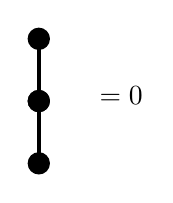
\begin{tikzpicture}[x=0.75pt,y=0.75pt,yscale=-1,xscale=1]
%uncomment if require: \path (0,513); %set diagram left start at 0, and has height of 513

%Straight Lines [id:da5455092391586145] 
\draw [line width=1.5]    (40,60) -- (40,30) ;
\draw [shift={(40,30)}, rotate = 270] [color={rgb, 255:red, 0; green, 0; blue, 0 }  ][fill={rgb, 255:red, 0; green, 0; blue, 0 }  ][line width=1.5]      (0, 0) circle [x radius= 4.36, y radius= 4.36]   ;
\draw [shift={(40,60)}, rotate = 270] [color={rgb, 255:red, 0; green, 0; blue, 0 }  ][fill={rgb, 255:red, 0; green, 0; blue, 0 }  ][line width=1.5]      (0, 0) circle [x radius= 4.36, y radius= 4.36]   ;
%Straight Lines [id:da552453933363283] 
\draw [line width=1.5]    (40,90) -- (40,60) ;
\draw [shift={(40,60)}, rotate = 270] [color={rgb, 255:red, 0; green, 0; blue, 0 }  ][fill={rgb, 255:red, 0; green, 0; blue, 0 }  ][line width=1.5]      (0, 0) circle [x radius= 4.36, y radius= 4.36]   ;
\draw [shift={(40,90)}, rotate = 270] [color={rgb, 255:red, 0; green, 0; blue, 0 }  ][fill={rgb, 255:red, 0; green, 0; blue, 0 }  ][line width=1.5]      (0, 0) circle [x radius= 4.36, y radius= 4.36]   ;

\draw (68,52) node [anchor=north west][inner sep=0.75pt]    {$= 0$};


\end{tikzpicture}    
\end{center}

just as we saw earlier for a general $\A$-algebra. The relation for $n=2$, is given by

% The second Stasheff identity for DG algebras using trees



\begin{center}
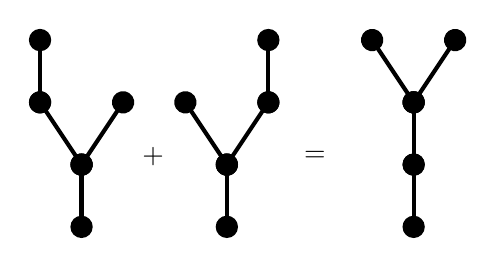
\begin{tikzpicture}[x=0.75pt,y=0.75pt,yscale=-1,xscale=1]
%uncomment if require: \path (0,513); %set diagram left start at 0, and has height of 513

%Straight Lines [id:da5455092391586145] 
\draw [line width=1.5]    (50,90) -- (30,60) ;
\draw [shift={(30,60)}, rotate = 236.31] [color={rgb, 255:red, 0; green, 0; blue, 0 }  ][fill={rgb, 255:red, 0; green, 0; blue, 0 }  ][line width=1.5]      (0, 0) circle [x radius= 4.36, y radius= 4.36]   ;
\draw [shift={(50,90)}, rotate = 236.31] [color={rgb, 255:red, 0; green, 0; blue, 0 }  ][fill={rgb, 255:red, 0; green, 0; blue, 0 }  ][line width=1.5]      (0, 0) circle [x radius= 4.36, y radius= 4.36]   ;
%Straight Lines [id:da552453933363283] 
\draw [line width=1.5]    (50,120) -- (50,90) ;
\draw [shift={(50,90)}, rotate = 270] [color={rgb, 255:red, 0; green, 0; blue, 0 }  ][fill={rgb, 255:red, 0; green, 0; blue, 0 }  ][line width=1.5]      (0, 0) circle [x radius= 4.36, y radius= 4.36]   ;
\draw [shift={(50,120)}, rotate = 270] [color={rgb, 255:red, 0; green, 0; blue, 0 }  ][fill={rgb, 255:red, 0; green, 0; blue, 0 }  ][line width=1.5]      (0, 0) circle [x radius= 4.36, y radius= 4.36]   ;
%Straight Lines [id:da4531423159403052] 
\draw [line width=1.5]    (50,90) -- (70,60) ;
\draw [shift={(70,60)}, rotate = 303.69] [color={rgb, 255:red, 0; green, 0; blue, 0 }  ][fill={rgb, 255:red, 0; green, 0; blue, 0 }  ][line width=1.5]      (0, 0) circle [x radius= 4.36, y radius= 4.36]   ;
\draw [shift={(50,90)}, rotate = 303.69] [color={rgb, 255:red, 0; green, 0; blue, 0 }  ][fill={rgb, 255:red, 0; green, 0; blue, 0 }  ][line width=1.5]      (0, 0) circle [x radius= 4.36, y radius= 4.36]   ;
%Straight Lines [id:da8658811299365152] 
\draw [line width=1.5]    (30,60) -- (30,30) ;
\draw [shift={(30,30)}, rotate = 270] [color={rgb, 255:red, 0; green, 0; blue, 0 }  ][fill={rgb, 255:red, 0; green, 0; blue, 0 }  ][line width=1.5]      (0, 0) circle [x radius= 4.36, y radius= 4.36]   ;
\draw [shift={(30,60)}, rotate = 270] [color={rgb, 255:red, 0; green, 0; blue, 0 }  ][fill={rgb, 255:red, 0; green, 0; blue, 0 }  ][line width=1.5]      (0, 0) circle [x radius= 4.36, y radius= 4.36]   ;
%Straight Lines [id:da9654905799619733] 
\draw [line width=1.5]    (120,90) -- (100,60) ;
\draw [shift={(100,60)}, rotate = 236.31] [color={rgb, 255:red, 0; green, 0; blue, 0 }  ][fill={rgb, 255:red, 0; green, 0; blue, 0 }  ][line width=1.5]      (0, 0) circle [x radius= 4.36, y radius= 4.36]   ;
\draw [shift={(120,90)}, rotate = 236.31] [color={rgb, 255:red, 0; green, 0; blue, 0 }  ][fill={rgb, 255:red, 0; green, 0; blue, 0 }  ][line width=1.5]      (0, 0) circle [x radius= 4.36, y radius= 4.36]   ;
%Straight Lines [id:da12989711620017252] 
\draw [line width=1.5]    (120,120) -- (120,90) ;
\draw [shift={(120,90)}, rotate = 270] [color={rgb, 255:red, 0; green, 0; blue, 0 }  ][fill={rgb, 255:red, 0; green, 0; blue, 0 }  ][line width=1.5]      (0, 0) circle [x radius= 4.36, y radius= 4.36]   ;
\draw [shift={(120,120)}, rotate = 270] [color={rgb, 255:red, 0; green, 0; blue, 0 }  ][fill={rgb, 255:red, 0; green, 0; blue, 0 }  ][line width=1.5]      (0, 0) circle [x radius= 4.36, y radius= 4.36]   ;
%Straight Lines [id:da316004338934887] 
\draw [line width=1.5]    (120,90) -- (140,60) ;
\draw [shift={(140,60)}, rotate = 303.69] [color={rgb, 255:red, 0; green, 0; blue, 0 }  ][fill={rgb, 255:red, 0; green, 0; blue, 0 }  ][line width=1.5]      (0, 0) circle [x radius= 4.36, y radius= 4.36]   ;
\draw [shift={(120,90)}, rotate = 303.69] [color={rgb, 255:red, 0; green, 0; blue, 0 }  ][fill={rgb, 255:red, 0; green, 0; blue, 0 }  ][line width=1.5]      (0, 0) circle [x radius= 4.36, y radius= 4.36]   ;
%Straight Lines [id:da4310585409341743] 
\draw [line width=1.5]    (140,60) -- (140,30) ;
\draw [shift={(140,30)}, rotate = 270] [color={rgb, 255:red, 0; green, 0; blue, 0 }  ][fill={rgb, 255:red, 0; green, 0; blue, 0 }  ][line width=1.5]      (0, 0) circle [x radius= 4.36, y radius= 4.36]   ;
\draw [shift={(140,60)}, rotate = 270] [color={rgb, 255:red, 0; green, 0; blue, 0 }  ][fill={rgb, 255:red, 0; green, 0; blue, 0 }  ][line width=1.5]      (0, 0) circle [x radius= 4.36, y radius= 4.36]   ;
%Straight Lines [id:da5694345020537597] 
\draw [line width=1.5]    (210,60) -- (190,30) ;
\draw [shift={(190,30)}, rotate = 236.31] [color={rgb, 255:red, 0; green, 0; blue, 0 }  ][fill={rgb, 255:red, 0; green, 0; blue, 0 }  ][line width=1.5]      (0, 0) circle [x radius= 4.36, y radius= 4.36]   ;
\draw [shift={(210,60)}, rotate = 236.31] [color={rgb, 255:red, 0; green, 0; blue, 0 }  ][fill={rgb, 255:red, 0; green, 0; blue, 0 }  ][line width=1.5]      (0, 0) circle [x radius= 4.36, y radius= 4.36]   ;
%Straight Lines [id:da353184704299615] 
\draw [line width=1.5]    (210,90) -- (210,60) ;
\draw [shift={(210,60)}, rotate = 270] [color={rgb, 255:red, 0; green, 0; blue, 0 }  ][fill={rgb, 255:red, 0; green, 0; blue, 0 }  ][line width=1.5]      (0, 0) circle [x radius= 4.36, y radius= 4.36]   ;
\draw [shift={(210,90)}, rotate = 270] [color={rgb, 255:red, 0; green, 0; blue, 0 }  ][fill={rgb, 255:red, 0; green, 0; blue, 0 }  ][line width=1.5]      (0, 0) circle [x radius= 4.36, y radius= 4.36]   ;
%Straight Lines [id:da8605408779697565] 
\draw [line width=1.5]    (210,60) -- (230,30) ;
\draw [shift={(230,30)}, rotate = 303.69] [color={rgb, 255:red, 0; green, 0; blue, 0 }  ][fill={rgb, 255:red, 0; green, 0; blue, 0 }  ][line width=1.5]      (0, 0) circle [x radius= 4.36, y radius= 4.36]   ;
\draw [shift={(210,60)}, rotate = 303.69] [color={rgb, 255:red, 0; green, 0; blue, 0 }  ][fill={rgb, 255:red, 0; green, 0; blue, 0 }  ][line width=1.5]      (0, 0) circle [x radius= 4.36, y radius= 4.36]   ;
%Straight Lines [id:da44074219568004036] 
\draw [line width=1.5]    (210,120) -- (210,90) ;
\draw [shift={(210,90)}, rotate = 270] [color={rgb, 255:red, 0; green, 0; blue, 0 }  ][fill={rgb, 255:red, 0; green, 0; blue, 0 }  ][line width=1.5]      (0, 0) circle [x radius= 4.36, y radius= 4.36]   ;
\draw [shift={(210,120)}, rotate = 270] [color={rgb, 255:red, 0; green, 0; blue, 0 }  ][fill={rgb, 255:red, 0; green, 0; blue, 0 }  ][line width=1.5]      (0, 0) circle [x radius= 4.36, y radius= 4.36]   ;

% Text Node
\draw (78,80.4) node [anchor=north west][inner sep=0.75pt]    {$+$};
% Text Node
\draw (156,82.4) node [anchor=north west][inner sep=0.75pt]    {$=$};


\end{tikzpicture}    
\end{center}

which we can recognize as the Leibniz rule. We don't have the $(-1)^{|x|}$ sign here, as it first arises when applying the Koszul grading rule when applying these operations to actual elements. The third and final relation is given by 

% The third Stasheff identity for DG algebras using trees



\begin{center}
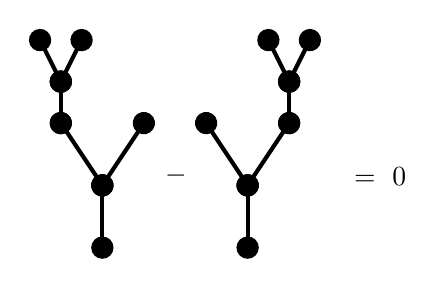
\begin{tikzpicture}[x=0.75pt,y=0.75pt,yscale=-1,xscale=1]
%uncomment if require: \path (0,513); %set diagram left start at 0, and has height of 513

%Straight Lines [id:da5455092391586145] 
\draw [line width=1.5]    (50,90) -- (30,60) ;
\draw [shift={(30,60)}, rotate = 236.31] [color={rgb, 255:red, 0; green, 0; blue, 0 }  ][fill={rgb, 255:red, 0; green, 0; blue, 0 }  ][line width=1.5]      (0, 0) circle [x radius= 4.36, y radius= 4.36]   ;
\draw [shift={(50,90)}, rotate = 236.31] [color={rgb, 255:red, 0; green, 0; blue, 0 }  ][fill={rgb, 255:red, 0; green, 0; blue, 0 }  ][line width=1.5]      (0, 0) circle [x radius= 4.36, y radius= 4.36]   ;
%Straight Lines [id:da552453933363283] 
\draw [line width=1.5]    (50,120) -- (50,90) ;
\draw [shift={(50,90)}, rotate = 270] [color={rgb, 255:red, 0; green, 0; blue, 0 }  ][fill={rgb, 255:red, 0; green, 0; blue, 0 }  ][line width=1.5]      (0, 0) circle [x radius= 4.36, y radius= 4.36]   ;
\draw [shift={(50,120)}, rotate = 270] [color={rgb, 255:red, 0; green, 0; blue, 0 }  ][fill={rgb, 255:red, 0; green, 0; blue, 0 }  ][line width=1.5]      (0, 0) circle [x radius= 4.36, y radius= 4.36]   ;
%Straight Lines [id:da4531423159403052] 
\draw [line width=1.5]    (50,90) -- (70,60) ;
\draw [shift={(70,60)}, rotate = 303.69] [color={rgb, 255:red, 0; green, 0; blue, 0 }  ][fill={rgb, 255:red, 0; green, 0; blue, 0 }  ][line width=1.5]      (0, 0) circle [x radius= 4.36, y radius= 4.36]   ;
\draw [shift={(50,90)}, rotate = 303.69] [color={rgb, 255:red, 0; green, 0; blue, 0 }  ][fill={rgb, 255:red, 0; green, 0; blue, 0 }  ][line width=1.5]      (0, 0) circle [x radius= 4.36, y radius= 4.36]   ;
%Straight Lines [id:da9654905799619733] 
\draw [line width=1.5]    (120,90) -- (100,60) ;
\draw [shift={(100,60)}, rotate = 236.31] [color={rgb, 255:red, 0; green, 0; blue, 0 }  ][fill={rgb, 255:red, 0; green, 0; blue, 0 }  ][line width=1.5]      (0, 0) circle [x radius= 4.36, y radius= 4.36]   ;
\draw [shift={(120,90)}, rotate = 236.31] [color={rgb, 255:red, 0; green, 0; blue, 0 }  ][fill={rgb, 255:red, 0; green, 0; blue, 0 }  ][line width=1.5]      (0, 0) circle [x radius= 4.36, y radius= 4.36]   ;
%Straight Lines [id:da12989711620017252] 
\draw [line width=1.5]    (120,120) -- (120,90) ;
\draw [shift={(120,90)}, rotate = 270] [color={rgb, 255:red, 0; green, 0; blue, 0 }  ][fill={rgb, 255:red, 0; green, 0; blue, 0 }  ][line width=1.5]      (0, 0) circle [x radius= 4.36, y radius= 4.36]   ;
\draw [shift={(120,120)}, rotate = 270] [color={rgb, 255:red, 0; green, 0; blue, 0 }  ][fill={rgb, 255:red, 0; green, 0; blue, 0 }  ][line width=1.5]      (0, 0) circle [x radius= 4.36, y radius= 4.36]   ;
%Straight Lines [id:da316004338934887] 
\draw [line width=1.5]    (120,90) -- (140,60) ;
\draw [shift={(140,60)}, rotate = 303.69] [color={rgb, 255:red, 0; green, 0; blue, 0 }  ][fill={rgb, 255:red, 0; green, 0; blue, 0 }  ][line width=1.5]      (0, 0) circle [x radius= 4.36, y radius= 4.36]   ;
\draw [shift={(120,90)}, rotate = 303.69] [color={rgb, 255:red, 0; green, 0; blue, 0 }  ][fill={rgb, 255:red, 0; green, 0; blue, 0 }  ][line width=1.5]      (0, 0) circle [x radius= 4.36, y radius= 4.36]   ;
%Straight Lines [id:da7774818944643269] 
\draw [line width=1.5]    (30,40) -- (20,20) ;
\draw [shift={(20,20)}, rotate = 243.43] [color={rgb, 255:red, 0; green, 0; blue, 0 }  ][fill={rgb, 255:red, 0; green, 0; blue, 0 }  ][line width=1.5]      (0, 0) circle [x radius= 4.36, y radius= 4.36]   ;
\draw [shift={(30,40)}, rotate = 243.43] [color={rgb, 255:red, 0; green, 0; blue, 0 }  ][fill={rgb, 255:red, 0; green, 0; blue, 0 }  ][line width=1.5]      (0, 0) circle [x radius= 4.36, y radius= 4.36]   ;
%Straight Lines [id:da04997050128847502] 
\draw [line width=1.5]    (30,60) -- (30,40) ;
\draw [shift={(30,40)}, rotate = 270] [color={rgb, 255:red, 0; green, 0; blue, 0 }  ][fill={rgb, 255:red, 0; green, 0; blue, 0 }  ][line width=1.5]      (0, 0) circle [x radius= 4.36, y radius= 4.36]   ;
\draw [shift={(30,60)}, rotate = 270] [color={rgb, 255:red, 0; green, 0; blue, 0 }  ][fill={rgb, 255:red, 0; green, 0; blue, 0 }  ][line width=1.5]      (0, 0) circle [x radius= 4.36, y radius= 4.36]   ;
%Straight Lines [id:da14436077290047278] 
\draw [line width=1.5]    (30,40) -- (40,20) ;
\draw [shift={(40,20)}, rotate = 296.57] [color={rgb, 255:red, 0; green, 0; blue, 0 }  ][fill={rgb, 255:red, 0; green, 0; blue, 0 }  ][line width=1.5]      (0, 0) circle [x radius= 4.36, y radius= 4.36]   ;
\draw [shift={(30,40)}, rotate = 296.57] [color={rgb, 255:red, 0; green, 0; blue, 0 }  ][fill={rgb, 255:red, 0; green, 0; blue, 0 }  ][line width=1.5]      (0, 0) circle [x radius= 4.36, y radius= 4.36]   ;
%Straight Lines [id:da9695689491811674] 
\draw [line width=1.5]    (140,40) -- (130,20) ;
\draw [shift={(130,20)}, rotate = 243.43] [color={rgb, 255:red, 0; green, 0; blue, 0 }  ][fill={rgb, 255:red, 0; green, 0; blue, 0 }  ][line width=1.5]      (0, 0) circle [x radius= 4.36, y radius= 4.36]   ;
\draw [shift={(140,40)}, rotate = 243.43] [color={rgb, 255:red, 0; green, 0; blue, 0 }  ][fill={rgb, 255:red, 0; green, 0; blue, 0 }  ][line width=1.5]      (0, 0) circle [x radius= 4.36, y radius= 4.36]   ;
%Straight Lines [id:da7408167553016403] 
\draw [line width=1.5]    (140,60) -- (140,40) ;
\draw [shift={(140,40)}, rotate = 270] [color={rgb, 255:red, 0; green, 0; blue, 0 }  ][fill={rgb, 255:red, 0; green, 0; blue, 0 }  ][line width=1.5]      (0, 0) circle [x radius= 4.36, y radius= 4.36]   ;
\draw [shift={(140,60)}, rotate = 270] [color={rgb, 255:red, 0; green, 0; blue, 0 }  ][fill={rgb, 255:red, 0; green, 0; blue, 0 }  ][line width=1.5]      (0, 0) circle [x radius= 4.36, y radius= 4.36]   ;
%Straight Lines [id:da11237732756013408] 
\draw [line width=1.5]    (140,40) -- (150,20) ;
\draw [shift={(150,20)}, rotate = 296.57] [color={rgb, 255:red, 0; green, 0; blue, 0 }  ][fill={rgb, 255:red, 0; green, 0; blue, 0 }  ][line width=1.5]      (0, 0) circle [x radius= 4.36, y radius= 4.36]   ;
\draw [shift={(140,40)}, rotate = 296.57] [color={rgb, 255:red, 0; green, 0; blue, 0 }  ][fill={rgb, 255:red, 0; green, 0; blue, 0 }  ][line width=1.5]      (0, 0) circle [x radius= 4.36, y radius= 4.36]   ;

% Text Node
\draw (79,79.4) node [anchor=north west][inner sep=0.75pt]    {$-$};
% Text Node
\draw (170,80.4) node [anchor=north west][inner sep=0.75pt]    {$=\ 0$};


\end{tikzpicture}    
\end{center}

which we recognize as the associativity condition.



\subsection{Visualization of morphisms using rooted trees}

We can also describe the relations of the $\A$-morphisms as systems of rooted trees. Let us assume we have a morphism of $\A$-algebras $f\colon A\longrightarrow B$. The idea is to compare what happens with applying the internal maps $m_n^A$ before applying the $f_i$'s versus first applying the $f_i$'s and then the internal maps $m_n^B$. Let's start with the former.

From the equation used to define the morphisms, we see that the left hand side is very similar to the Stasheff identities. In fact, it is exactly what we get if we replace the operation $m_{r+1+t}^A$ by $f_{r+1+t}$, i.e. 
\begin{equation*}
    \sum_{n = r+s+t}(-1)^{r+st}f_{r+1+t}(id^{\otimes r}\otimes m_s^A \otimes id^{\otimes t}).
\end{equation*}

To differentiate the $f_i$'s from the $m_n$'s we use a white dots in the central vertex to represent $f_i$, and the same black dots as before to represent the $m_n$'s, for example:


% Notation of morphisms vs operations

\begin{center}
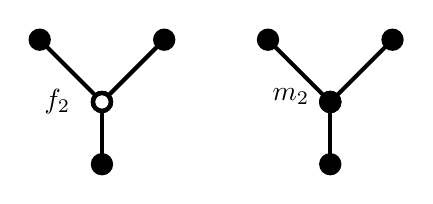
\begin{tikzpicture}[x=0.75pt,y=0.75pt,yscale=-1,xscale=1]
%uncomment if require: \path (0,513); %set diagram left start at 0, and has height of 513

%Straight Lines [id:da22704499488399277] 
\draw [line width=1.5]    (127.63,97.63) -- (100,70) ;
\draw [shift={(100,70)}, rotate = 225] [color={rgb, 255:red, 0; green, 0; blue, 0 }  ][fill={rgb, 255:red, 0; green, 0; blue, 0 }  ][line width=1.5]      (0, 0) circle [x radius= 4.36, y radius= 4.36]   ;
\draw [shift={(130,100)}, rotate = 225] [color={rgb, 255:red, 0; green, 0; blue, 0 }  ][line width=1.5]      (0, 0) circle [x radius= 4.36, y radius= 4.36]   ;
%Straight Lines [id:da6600645534832517] 
\draw [line width=1.5]    (132.37,97.63) -- (160,70) ;
\draw [shift={(160,70)}, rotate = 315] [color={rgb, 255:red, 0; green, 0; blue, 0 }  ][fill={rgb, 255:red, 0; green, 0; blue, 0 }  ][line width=1.5]      (0, 0) circle [x radius= 4.36, y radius= 4.36]   ;
\draw [shift={(130,100)}, rotate = 315] [color={rgb, 255:red, 0; green, 0; blue, 0 }  ][line width=1.5]      (0, 0) circle [x radius= 4.36, y radius= 4.36]   ;
%Straight Lines [id:da5336563710509243] 
\draw [line width=1.5]    (130,130) -- (130,103.35) ;
\draw [shift={(130,100)}, rotate = 270] [color={rgb, 255:red, 0; green, 0; blue, 0 }  ][line width=1.5]      (0, 0) circle [x radius= 4.36, y radius= 4.36]   ;
\draw [shift={(130,130)}, rotate = 270] [color={rgb, 255:red, 0; green, 0; blue, 0 }  ][fill={rgb, 255:red, 0; green, 0; blue, 0 }  ][line width=1.5]      (0, 0) circle [x radius= 4.36, y radius= 4.36]   ;
%Straight Lines [id:da8291560339264339] 
\draw [line width=1.5]    (240,100) -- (210,70) ;
\draw [shift={(210,70)}, rotate = 225] [color={rgb, 255:red, 0; green, 0; blue, 0 }  ][fill={rgb, 255:red, 0; green, 0; blue, 0 }  ][line width=1.5]      (0, 0) circle [x radius= 4.36, y radius= 4.36]   ;
\draw [shift={(240,100)}, rotate = 225] [color={rgb, 255:red, 0; green, 0; blue, 0 }  ][fill={rgb, 255:red, 0; green, 0; blue, 0 }  ][line width=1.5]      (0, 0) circle [x radius= 4.36, y radius= 4.36]   ;
%Straight Lines [id:da49852005608074124] 
\draw [line width=1.5]    (240,100) -- (270,70) ;
\draw [shift={(270,70)}, rotate = 315] [color={rgb, 255:red, 0; green, 0; blue, 0 }  ][fill={rgb, 255:red, 0; green, 0; blue, 0 }  ][line width=1.5]      (0, 0) circle [x radius= 4.36, y radius= 4.36]   ;
\draw [shift={(240,100)}, rotate = 315] [color={rgb, 255:red, 0; green, 0; blue, 0 }  ][fill={rgb, 255:red, 0; green, 0; blue, 0 }  ][line width=1.5]      (0, 0) circle [x radius= 4.36, y radius= 4.36]   ;
%Straight Lines [id:da02571865044906385] 
\draw [line width=1.5]    (240,130) -- (240,100) ;
\draw [shift={(240,100)}, rotate = 270] [color={rgb, 255:red, 0; green, 0; blue, 0 }  ][fill={rgb, 255:red, 0; green, 0; blue, 0 }  ][line width=1.5]      (0, 0) circle [x radius= 4.36, y radius= 4.36]   ;
\draw [shift={(240,130)}, rotate = 270] [color={rgb, 255:red, 0; green, 0; blue, 0 }  ][fill={rgb, 255:red, 0; green, 0; blue, 0 }  ][line width=1.5]      (0, 0) circle [x radius= 4.36, y radius= 4.36]   ;

% Text Node
\draw (101,92.4) node [anchor=north west][inner sep=0.75pt]    {$f_{2}$};
% Text Node
\draw (211,92.4) node [anchor=north west][inner sep=0.75pt]    {$m_{2}$};

\end{tikzpicture}
\end{center}

We then do exactly the same procedure as we did when constructing the trees for the different compositions of the $m_n$'s. For $n=1$ we get 

% Left part of the first Stasheff identity for morphisms



\begin{center}
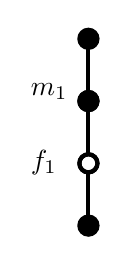
\begin{tikzpicture}[x=0.75pt,y=0.75pt,yscale=-1,xscale=1]
%uncomment if require: \path (0,513); %set diagram left start at 0, and has height of 513

%Straight Lines [id:da6600645534832517] 
\draw [line width=1.5]    (130,96.65) -- (130,70) ;
\draw [shift={(130,70)}, rotate = 270] [color={rgb, 255:red, 0; green, 0; blue, 0 }  ][fill={rgb, 255:red, 0; green, 0; blue, 0 }  ][line width=1.5]      (0, 0) circle [x radius= 4.36, y radius= 4.36]   ;
\draw [shift={(130,100)}, rotate = 270] [color={rgb, 255:red, 0; green, 0; blue, 0 }  ][line width=1.5]      (0, 0) circle [x radius= 4.36, y radius= 4.36]   ;
%Straight Lines [id:da5336563710509243] 
\draw [line width=1.5]    (130,130) -- (130,103.35) ;
\draw [shift={(130,100)}, rotate = 270] [color={rgb, 255:red, 0; green, 0; blue, 0 }  ][line width=1.5]      (0, 0) circle [x radius= 4.36, y radius= 4.36]   ;
\draw [shift={(130,130)}, rotate = 270] [color={rgb, 255:red, 0; green, 0; blue, 0 }  ][fill={rgb, 255:red, 0; green, 0; blue, 0 }  ][line width=1.5]      (0, 0) circle [x radius= 4.36, y radius= 4.36]   ;
%Straight Lines [id:da09838053140717373] 
\draw [line width=1.5]    (130,70) -- (130,40) ;
\draw [shift={(130,40)}, rotate = 270] [color={rgb, 255:red, 0; green, 0; blue, 0 }  ][fill={rgb, 255:red, 0; green, 0; blue, 0 }  ][line width=1.5]      (0, 0) circle [x radius= 4.36, y radius= 4.36]   ;
\draw [shift={(130,70)}, rotate = 270] [color={rgb, 255:red, 0; green, 0; blue, 0 }  ][fill={rgb, 255:red, 0; green, 0; blue, 0 }  ][line width=1.5]      (0, 0) circle [x radius= 4.36, y radius= 4.36]   ;

% Text Node
\draw (101,92.4) node [anchor=north west][inner sep=0.75pt]    {$f_{1}$};
% Text Node
\draw (101,60.4) node [anchor=north west][inner sep=0.75pt]    {$m_{1}$};


\end{tikzpicture}
   
\end{center}

For $n=2$ we get three different parts. We now stop labeling the different parts, and instead read them out from the trees themselves. We get

% Left part of the second Stasheff identity for morphisms without signs



\begin{center}
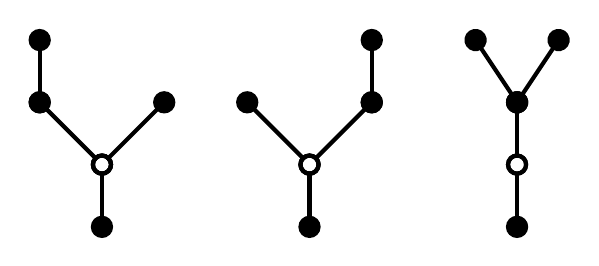
\begin{tikzpicture}[x=0.75pt,y=0.75pt,yscale=-1,xscale=1]
%uncomment if require: \path (0,513); %set diagram left start at 0, and has height of 513

%Straight Lines [id:da22704499488399277] 
\draw [line width=1.5]    (87.63,97.63) -- (60,70) ;
\draw [shift={(60,70)}, rotate = 225] [color={rgb, 255:red, 0; green, 0; blue, 0 }  ][fill={rgb, 255:red, 0; green, 0; blue, 0 }  ][line width=1.5]      (0, 0) circle [x radius= 4.36, y radius= 4.36]   ;
\draw [shift={(90,100)}, rotate = 225] [color={rgb, 255:red, 0; green, 0; blue, 0 }  ][line width=1.5]      (0, 0) circle [x radius= 4.36, y radius= 4.36]   ;
%Straight Lines [id:da6600645534832517] 
\draw [line width=1.5]    (92.37,97.63) -- (120,70) ;
\draw [shift={(120,70)}, rotate = 315] [color={rgb, 255:red, 0; green, 0; blue, 0 }  ][fill={rgb, 255:red, 0; green, 0; blue, 0 }  ][line width=1.5]      (0, 0) circle [x radius= 4.36, y radius= 4.36]   ;
\draw [shift={(90,100)}, rotate = 315] [color={rgb, 255:red, 0; green, 0; blue, 0 }  ][line width=1.5]      (0, 0) circle [x radius= 4.36, y radius= 4.36]   ;
%Straight Lines [id:da5336563710509243] 
\draw [line width=1.5]    (90,130) -- (90,103.35) ;
\draw [shift={(90,100)}, rotate = 270] [color={rgb, 255:red, 0; green, 0; blue, 0 }  ][line width=1.5]      (0, 0) circle [x radius= 4.36, y radius= 4.36]   ;
\draw [shift={(90,130)}, rotate = 270] [color={rgb, 255:red, 0; green, 0; blue, 0 }  ][fill={rgb, 255:red, 0; green, 0; blue, 0 }  ][line width=1.5]      (0, 0) circle [x radius= 4.36, y radius= 4.36]   ;
%Straight Lines [id:da02571865044906385] 
\draw [line width=1.5]    (60,70) -- (60,40) ;
\draw [shift={(60,40)}, rotate = 270] [color={rgb, 255:red, 0; green, 0; blue, 0 }  ][fill={rgb, 255:red, 0; green, 0; blue, 0 }  ][line width=1.5]      (0, 0) circle [x radius= 4.36, y radius= 4.36]   ;
\draw [shift={(60,70)}, rotate = 270] [color={rgb, 255:red, 0; green, 0; blue, 0 }  ][fill={rgb, 255:red, 0; green, 0; blue, 0 }  ][line width=1.5]      (0, 0) circle [x radius= 4.36, y radius= 4.36]   ;
%Straight Lines [id:da12304237726374523] 
\draw [line width=1.5]    (187.63,97.63) -- (160,70) ;
\draw [shift={(160,70)}, rotate = 225] [color={rgb, 255:red, 0; green, 0; blue, 0 }  ][fill={rgb, 255:red, 0; green, 0; blue, 0 }  ][line width=1.5]      (0, 0) circle [x radius= 4.36, y radius= 4.36]   ;
\draw [shift={(190,100)}, rotate = 225] [color={rgb, 255:red, 0; green, 0; blue, 0 }  ][line width=1.5]      (0, 0) circle [x radius= 4.36, y radius= 4.36]   ;
%Straight Lines [id:da1480022122503979] 
\draw [line width=1.5]    (192.37,97.63) -- (220,70) ;
\draw [shift={(220,70)}, rotate = 315] [color={rgb, 255:red, 0; green, 0; blue, 0 }  ][fill={rgb, 255:red, 0; green, 0; blue, 0 }  ][line width=1.5]      (0, 0) circle [x radius= 4.36, y radius= 4.36]   ;
\draw [shift={(190,100)}, rotate = 315] [color={rgb, 255:red, 0; green, 0; blue, 0 }  ][line width=1.5]      (0, 0) circle [x radius= 4.36, y radius= 4.36]   ;
%Straight Lines [id:da31077771870320836] 
\draw [line width=1.5]    (190,130) -- (190,103.35) ;
\draw [shift={(190,100)}, rotate = 270] [color={rgb, 255:red, 0; green, 0; blue, 0 }  ][line width=1.5]      (0, 0) circle [x radius= 4.36, y radius= 4.36]   ;
\draw [shift={(190,130)}, rotate = 270] [color={rgb, 255:red, 0; green, 0; blue, 0 }  ][fill={rgb, 255:red, 0; green, 0; blue, 0 }  ][line width=1.5]      (0, 0) circle [x radius= 4.36, y radius= 4.36]   ;
%Straight Lines [id:da472311397338814] 
\draw [line width=1.5]    (220,70) -- (220,40) ;
\draw [shift={(220,40)}, rotate = 270] [color={rgb, 255:red, 0; green, 0; blue, 0 }  ][fill={rgb, 255:red, 0; green, 0; blue, 0 }  ][line width=1.5]      (0, 0) circle [x radius= 4.36, y radius= 4.36]   ;
\draw [shift={(220,70)}, rotate = 270] [color={rgb, 255:red, 0; green, 0; blue, 0 }  ][fill={rgb, 255:red, 0; green, 0; blue, 0 }  ][line width=1.5]      (0, 0) circle [x radius= 4.36, y radius= 4.36]   ;
%Straight Lines [id:da248153808508637] 
\draw [line width=1.5]    (290,130) -- (290,103.35) ;
\draw [shift={(290,100)}, rotate = 270] [color={rgb, 255:red, 0; green, 0; blue, 0 }  ][line width=1.5]      (0, 0) circle [x radius= 4.36, y radius= 4.36]   ;
\draw [shift={(290,130)}, rotate = 270] [color={rgb, 255:red, 0; green, 0; blue, 0 }  ][fill={rgb, 255:red, 0; green, 0; blue, 0 }  ][line width=1.5]      (0, 0) circle [x radius= 4.36, y radius= 4.36]   ;
%Straight Lines [id:da7635207194296745] 
\draw [line width=1.5]    (290,70) -- (270,40) ;
\draw [shift={(270,40)}, rotate = 236.31] [color={rgb, 255:red, 0; green, 0; blue, 0 }  ][fill={rgb, 255:red, 0; green, 0; blue, 0 }  ][line width=1.5]      (0, 0) circle [x radius= 4.36, y radius= 4.36]   ;
\draw [shift={(290,70)}, rotate = 236.31] [color={rgb, 255:red, 0; green, 0; blue, 0 }  ][fill={rgb, 255:red, 0; green, 0; blue, 0 }  ][line width=1.5]      (0, 0) circle [x radius= 4.36, y radius= 4.36]   ;
%Straight Lines [id:da7588798966530494] 
\draw [line width=1.5]    (290,70) -- (310,40) ;
\draw [shift={(310,40)}, rotate = 303.69] [color={rgb, 255:red, 0; green, 0; blue, 0 }  ][fill={rgb, 255:red, 0; green, 0; blue, 0 }  ][line width=1.5]      (0, 0) circle [x radius= 4.36, y radius= 4.36]   ;
\draw [shift={(290,70)}, rotate = 303.69] [color={rgb, 255:red, 0; green, 0; blue, 0 }  ][fill={rgb, 255:red, 0; green, 0; blue, 0 }  ][line width=1.5]      (0, 0) circle [x radius= 4.36, y radius= 4.36]   ;
%Straight Lines [id:da27750912598501865] 
\draw [line width=1.5]    (290,96.65) -- (290,70) ;
\draw [shift={(290,70)}, rotate = 270] [color={rgb, 255:red, 0; green, 0; blue, 0 }  ][fill={rgb, 255:red, 0; green, 0; blue, 0 }  ][line width=1.5]      (0, 0) circle [x radius= 4.36, y radius= 4.36]   ;
\draw [shift={(290,100)}, rotate = 270] [color={rgb, 255:red, 0; green, 0; blue, 0 }  ][line width=1.5]      (0, 0) circle [x radius= 4.36, y radius= 4.36]   ;

% Text Node
%\draw (61,92.4) node [anchor=north west][inner sep=0.75pt]    {$f_{2}$};
% Text Node
%\draw (33,46.4) node [anchor=north west][inner sep=0.75pt]    {$m_{1}$};
% Text Node
%\draw (161,92.4) node [anchor=north west][inner sep=0.75pt]    {$f_{2}$};
% Text Node
%\draw (194,45.4) node [anchor=north west][inner sep=0.75pt]    {$m_{1}$};
% Text Node
%\draw (261,61.4) node [anchor=north west][inner sep=0.75pt]    {$m_{2}$};
% Text Node
%\draw (261,90.4) node [anchor=north west][inner sep=0.75pt]    {$f_{1}$};


\end{tikzpicture}

\end{center}

To figure out the signs we can do exactly the same as for the Stasheff identities. Put the trees in a upside-down triangle and alternate placing constant signs and alternating signs. For $n=2$ we get the following

% Left part of the second Stasheff identity for morphisms with signs


\begin{center}
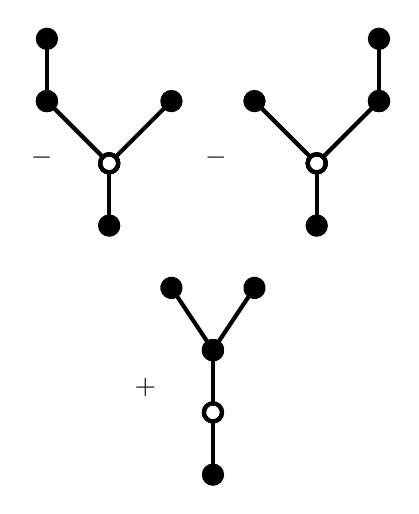
\begin{tikzpicture}[x=0.75pt,y=0.75pt,yscale=-1,xscale=1]
%uncomment if require: \path (0,513); %set diagram left start at 0, and has height of 513

%Straight Lines [id:da22704499488399277] 
\draw [line width=1.5]    (87.63,97.63) -- (60,70) ;
\draw [shift={(60,70)}, rotate = 225] [color={rgb, 255:red, 0; green, 0; blue, 0 }  ][fill={rgb, 255:red, 0; green, 0; blue, 0 }  ][line width=1.5]      (0, 0) circle [x radius= 4.36, y radius= 4.36]   ;
\draw [shift={(90,100)}, rotate = 225] [color={rgb, 255:red, 0; green, 0; blue, 0 }  ][line width=1.5]      (0, 0) circle [x radius= 4.36, y radius= 4.36]   ;
%Straight Lines [id:da6600645534832517] 
\draw [line width=1.5]    (92.37,97.63) -- (120,70) ;
\draw [shift={(120,70)}, rotate = 315] [color={rgb, 255:red, 0; green, 0; blue, 0 }  ][fill={rgb, 255:red, 0; green, 0; blue, 0 }  ][line width=1.5]      (0, 0) circle [x radius= 4.36, y radius= 4.36]   ;
\draw [shift={(90,100)}, rotate = 315] [color={rgb, 255:red, 0; green, 0; blue, 0 }  ][line width=1.5]      (0, 0) circle [x radius= 4.36, y radius= 4.36]   ;
%Straight Lines [id:da5336563710509243] 
\draw [line width=1.5]    (90,130) -- (90,103.35) ;
\draw [shift={(90,100)}, rotate = 270] [color={rgb, 255:red, 0; green, 0; blue, 0 }  ][line width=1.5]      (0, 0) circle [x radius= 4.36, y radius= 4.36]   ;
\draw [shift={(90,130)}, rotate = 270] [color={rgb, 255:red, 0; green, 0; blue, 0 }  ][fill={rgb, 255:red, 0; green, 0; blue, 0 }  ][line width=1.5]      (0, 0) circle [x radius= 4.36, y radius= 4.36]   ;
%Straight Lines [id:da02571865044906385] 
\draw [line width=1.5]    (60,70) -- (60,40) ;
\draw [shift={(60,40)}, rotate = 270] [color={rgb, 255:red, 0; green, 0; blue, 0 }  ][fill={rgb, 255:red, 0; green, 0; blue, 0 }  ][line width=1.5]      (0, 0) circle [x radius= 4.36, y radius= 4.36]   ;
\draw [shift={(60,70)}, rotate = 270] [color={rgb, 255:red, 0; green, 0; blue, 0 }  ][fill={rgb, 255:red, 0; green, 0; blue, 0 }  ][line width=1.5]      (0, 0) circle [x radius= 4.36, y radius= 4.36]   ;
%Straight Lines [id:da12304237726374523] 
\draw [line width=1.5]    (187.63,97.63) -- (160,70) ;
\draw [shift={(160,70)}, rotate = 225] [color={rgb, 255:red, 0; green, 0; blue, 0 }  ][fill={rgb, 255:red, 0; green, 0; blue, 0 }  ][line width=1.5]      (0, 0) circle [x radius= 4.36, y radius= 4.36]   ;
\draw [shift={(190,100)}, rotate = 225] [color={rgb, 255:red, 0; green, 0; blue, 0 }  ][line width=1.5]      (0, 0) circle [x radius= 4.36, y radius= 4.36]   ;
%Straight Lines [id:da1480022122503979] 
\draw [line width=1.5]    (192.37,97.63) -- (220,70) ;
\draw [shift={(220,70)}, rotate = 315] [color={rgb, 255:red, 0; green, 0; blue, 0 }  ][fill={rgb, 255:red, 0; green, 0; blue, 0 }  ][line width=1.5]      (0, 0) circle [x radius= 4.36, y radius= 4.36]   ;
\draw [shift={(190,100)}, rotate = 315] [color={rgb, 255:red, 0; green, 0; blue, 0 }  ][line width=1.5]      (0, 0) circle [x radius= 4.36, y radius= 4.36]   ;
%Straight Lines [id:da31077771870320836] 
\draw [line width=1.5]    (190,130) -- (190,103.35) ;
\draw [shift={(190,100)}, rotate = 270] [color={rgb, 255:red, 0; green, 0; blue, 0 }  ][line width=1.5]      (0, 0) circle [x radius= 4.36, y radius= 4.36]   ;
\draw [shift={(190,130)}, rotate = 270] [color={rgb, 255:red, 0; green, 0; blue, 0 }  ][fill={rgb, 255:red, 0; green, 0; blue, 0 }  ][line width=1.5]      (0, 0) circle [x radius= 4.36, y radius= 4.36]   ;
%Straight Lines [id:da472311397338814] 
\draw [line width=1.5]    (220,70) -- (220,40) ;
\draw [shift={(220,40)}, rotate = 270] [color={rgb, 255:red, 0; green, 0; blue, 0 }  ][fill={rgb, 255:red, 0; green, 0; blue, 0 }  ][line width=1.5]      (0, 0) circle [x radius= 4.36, y radius= 4.36]   ;
\draw [shift={(220,70)}, rotate = 270] [color={rgb, 255:red, 0; green, 0; blue, 0 }  ][fill={rgb, 255:red, 0; green, 0; blue, 0 }  ][line width=1.5]      (0, 0) circle [x radius= 4.36, y radius= 4.36]   ;
%Straight Lines [id:da248153808508637] 
\draw [line width=1.5]    (140,250) -- (140,223.36) ;
\draw [shift={(140,220)}, rotate = 270] [color={rgb, 255:red, 0; green, 0; blue, 0 }  ][line width=1.5]      (0, 0) circle [x radius= 4.36, y radius= 4.36]   ;
\draw [shift={(140,250)}, rotate = 270] [color={rgb, 255:red, 0; green, 0; blue, 0 }  ][fill={rgb, 255:red, 0; green, 0; blue, 0 }  ][line width=1.5]      (0, 0) circle [x radius= 4.36, y radius= 4.36]   ;
%Straight Lines [id:da7635207194296745] 
\draw [line width=1.5]    (140,190) -- (120,160) ;
\draw [shift={(120,160)}, rotate = 236.31] [color={rgb, 255:red, 0; green, 0; blue, 0 }  ][fill={rgb, 255:red, 0; green, 0; blue, 0 }  ][line width=1.5]      (0, 0) circle [x radius= 4.36, y radius= 4.36]   ;
\draw [shift={(140,190)}, rotate = 236.31] [color={rgb, 255:red, 0; green, 0; blue, 0 }  ][fill={rgb, 255:red, 0; green, 0; blue, 0 }  ][line width=1.5]      (0, 0) circle [x radius= 4.36, y radius= 4.36]   ;
%Straight Lines [id:da7588798966530494] 
\draw [line width=1.5]    (140,190) -- (160,160) ;
\draw [shift={(160,160)}, rotate = 303.69] [color={rgb, 255:red, 0; green, 0; blue, 0 }  ][fill={rgb, 255:red, 0; green, 0; blue, 0 }  ][line width=1.5]      (0, 0) circle [x radius= 4.36, y radius= 4.36]   ;
\draw [shift={(140,190)}, rotate = 303.69] [color={rgb, 255:red, 0; green, 0; blue, 0 }  ][fill={rgb, 255:red, 0; green, 0; blue, 0 }  ][line width=1.5]      (0, 0) circle [x radius= 4.36, y radius= 4.36]   ;
%Straight Lines [id:da27750912598501865] 
\draw [line width=1.5]    (140,216.65) -- (140,190) ;
\draw [shift={(140,190)}, rotate = 270] [color={rgb, 255:red, 0; green, 0; blue, 0 }  ][fill={rgb, 255:red, 0; green, 0; blue, 0 }  ][line width=1.5]      (0, 0) circle [x radius= 4.36, y radius= 4.36]   ;
\draw [shift={(140,220)}, rotate = 270] [color={rgb, 255:red, 0; green, 0; blue, 0 }  ][line width=1.5]      (0, 0) circle [x radius= 4.36, y radius= 4.36]   ;

% Text Node
\draw (51,91.4) node [anchor=north west][inner sep=0.75pt]    {$-$};
% Text Node
\draw (135,91.4) node [anchor=north west][inner sep=0.75pt]    {$-$};
% Text Node
\draw (101,202.4) node [anchor=north west][inner sep=0.75pt]    {$+$};


\end{tikzpicture}
\end{center}

Because of the nice aesthetics, and because we skipped straight to $n=4$ for the Stasheff identities, we include the system we get for $n=3$:


% The left part of the third Stasheff identity for morphisms with signs


\begin{center}
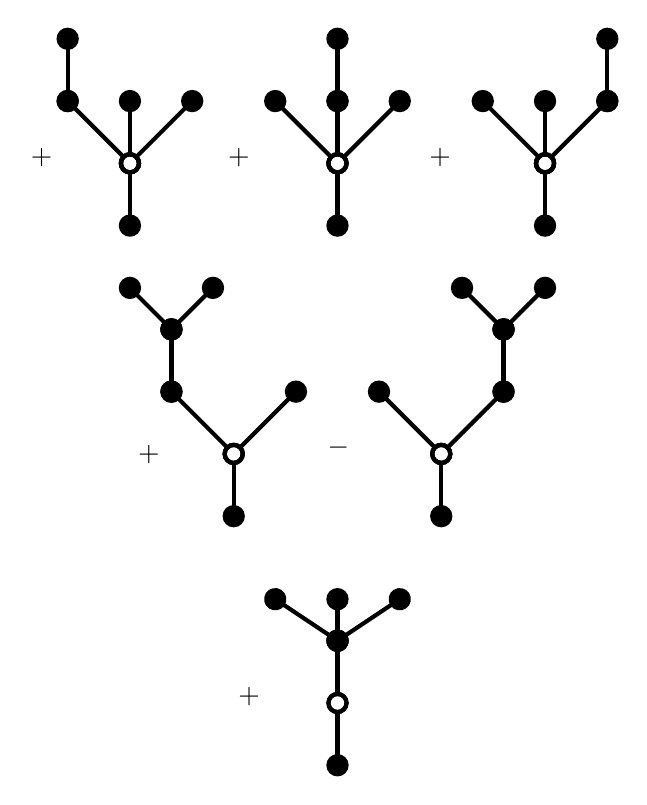
\begin{tikzpicture}[x=0.75pt,y=0.75pt,yscale=-1,xscale=1]
%uncomment if require: \path (0,513); %set diagram left start at 0, and has height of 513

%Straight Lines [id:da5027840919946027] 
\draw [line width=1.5]    (47.63,77.63) -- (20,50) ;
\draw [shift={(20,50)}, rotate = 225] [color={rgb, 255:red, 0; green, 0; blue, 0 }  ][fill={rgb, 255:red, 0; green, 0; blue, 0 }  ][line width=1.5]      (0, 0) circle [x radius= 4.36, y radius= 4.36]   ;
\draw [shift={(50,80)}, rotate = 225] [color={rgb, 255:red, 0; green, 0; blue, 0 }  ][line width=1.5]      (0, 0) circle [x radius= 4.36, y radius= 4.36]   ;
%Straight Lines [id:da012169408330350517] 
\draw [line width=1.5]    (50,76.65) -- (50,50) ;
\draw [shift={(50,50)}, rotate = 270] [color={rgb, 255:red, 0; green, 0; blue, 0 }  ][fill={rgb, 255:red, 0; green, 0; blue, 0 }  ][line width=1.5]      (0, 0) circle [x radius= 4.36, y radius= 4.36]   ;
\draw [shift={(50,80)}, rotate = 270] [color={rgb, 255:red, 0; green, 0; blue, 0 }  ][line width=1.5]      (0, 0) circle [x radius= 4.36, y radius= 4.36]   ;
%Straight Lines [id:da3794956070144304] 
\draw [line width=1.5]    (52.37,77.63) -- (80,50) ;
\draw [shift={(80,50)}, rotate = 315] [color={rgb, 255:red, 0; green, 0; blue, 0 }  ][fill={rgb, 255:red, 0; green, 0; blue, 0 }  ][line width=1.5]      (0, 0) circle [x radius= 4.36, y radius= 4.36]   ;
\draw [shift={(50,80)}, rotate = 315] [color={rgb, 255:red, 0; green, 0; blue, 0 }  ][line width=1.5]      (0, 0) circle [x radius= 4.36, y radius= 4.36]   ;
%Straight Lines [id:da8996197602070666] 
\draw [line width=1.5]    (50,110) -- (50,83.35) ;
\draw [shift={(50,80)}, rotate = 270] [color={rgb, 255:red, 0; green, 0; blue, 0 }  ][line width=1.5]      (0, 0) circle [x radius= 4.36, y radius= 4.36]   ;
\draw [shift={(50,110)}, rotate = 270] [color={rgb, 255:red, 0; green, 0; blue, 0 }  ][fill={rgb, 255:red, 0; green, 0; blue, 0 }  ][line width=1.5]      (0, 0) circle [x radius= 4.36, y radius= 4.36]   ;
%Straight Lines [id:da37599967010410107] 
\draw [line width=1.5]    (20,50) -- (20,20) ;
\draw [shift={(20,20)}, rotate = 270] [color={rgb, 255:red, 0; green, 0; blue, 0 }  ][fill={rgb, 255:red, 0; green, 0; blue, 0 }  ][line width=1.5]      (0, 0) circle [x radius= 4.36, y radius= 4.36]   ;
\draw [shift={(20,50)}, rotate = 270] [color={rgb, 255:red, 0; green, 0; blue, 0 }  ][fill={rgb, 255:red, 0; green, 0; blue, 0 }  ][line width=1.5]      (0, 0) circle [x radius= 4.36, y radius= 4.36]   ;
%Straight Lines [id:da698265177656928] 
\draw [line width=1.5]    (147.63,77.63) -- (120,50) ;
\draw [shift={(120,50)}, rotate = 225] [color={rgb, 255:red, 0; green, 0; blue, 0 }  ][fill={rgb, 255:red, 0; green, 0; blue, 0 }  ][line width=1.5]      (0, 0) circle [x radius= 4.36, y radius= 4.36]   ;
\draw [shift={(150,80)}, rotate = 225] [color={rgb, 255:red, 0; green, 0; blue, 0 }  ][line width=1.5]      (0, 0) circle [x radius= 4.36, y radius= 4.36]   ;
%Straight Lines [id:da049456703112388256] 
\draw [line width=1.5]    (150,76.65) -- (150,50) ;
\draw [shift={(150,50)}, rotate = 270] [color={rgb, 255:red, 0; green, 0; blue, 0 }  ][fill={rgb, 255:red, 0; green, 0; blue, 0 }  ][line width=1.5]      (0, 0) circle [x radius= 4.36, y radius= 4.36]   ;
\draw [shift={(150,80)}, rotate = 270] [color={rgb, 255:red, 0; green, 0; blue, 0 }  ][line width=1.5]      (0, 0) circle [x radius= 4.36, y radius= 4.36]   ;
%Straight Lines [id:da19781405329398405] 
\draw [line width=1.5]    (152.37,77.63) -- (180,50) ;
\draw [shift={(180,50)}, rotate = 315] [color={rgb, 255:red, 0; green, 0; blue, 0 }  ][fill={rgb, 255:red, 0; green, 0; blue, 0 }  ][line width=1.5]      (0, 0) circle [x radius= 4.36, y radius= 4.36]   ;
\draw [shift={(150,80)}, rotate = 315] [color={rgb, 255:red, 0; green, 0; blue, 0 }  ][line width=1.5]      (0, 0) circle [x radius= 4.36, y radius= 4.36]   ;
%Straight Lines [id:da9771660287757578] 
\draw [line width=1.5]    (150,110) -- (150,83.35) ;
\draw [shift={(150,80)}, rotate = 270] [color={rgb, 255:red, 0; green, 0; blue, 0 }  ][line width=1.5]      (0, 0) circle [x radius= 4.36, y radius= 4.36]   ;
\draw [shift={(150,110)}, rotate = 270] [color={rgb, 255:red, 0; green, 0; blue, 0 }  ][fill={rgb, 255:red, 0; green, 0; blue, 0 }  ][line width=1.5]      (0, 0) circle [x radius= 4.36, y radius= 4.36]   ;
%Straight Lines [id:da01581391478939298] 
\draw [line width=1.5]    (150,50) -- (150,20) ;
\draw [shift={(150,20)}, rotate = 270] [color={rgb, 255:red, 0; green, 0; blue, 0 }  ][fill={rgb, 255:red, 0; green, 0; blue, 0 }  ][line width=1.5]      (0, 0) circle [x radius= 4.36, y radius= 4.36]   ;
\draw [shift={(150,50)}, rotate = 270] [color={rgb, 255:red, 0; green, 0; blue, 0 }  ][fill={rgb, 255:red, 0; green, 0; blue, 0 }  ][line width=1.5]      (0, 0) circle [x radius= 4.36, y radius= 4.36]   ;
%Straight Lines [id:da39290163971213876] 
\draw [line width=1.5]    (247.63,77.63) -- (220,50) ;
\draw [shift={(220,50)}, rotate = 225] [color={rgb, 255:red, 0; green, 0; blue, 0 }  ][fill={rgb, 255:red, 0; green, 0; blue, 0 }  ][line width=1.5]      (0, 0) circle [x radius= 4.36, y radius= 4.36]   ;
\draw [shift={(250,80)}, rotate = 225] [color={rgb, 255:red, 0; green, 0; blue, 0 }  ][line width=1.5]      (0, 0) circle [x radius= 4.36, y radius= 4.36]   ;
%Straight Lines [id:da6585976068778385] 
\draw [line width=1.5]    (250,76.65) -- (250,50) ;
\draw [shift={(250,50)}, rotate = 270] [color={rgb, 255:red, 0; green, 0; blue, 0 }  ][fill={rgb, 255:red, 0; green, 0; blue, 0 }  ][line width=1.5]      (0, 0) circle [x radius= 4.36, y radius= 4.36]   ;
\draw [shift={(250,80)}, rotate = 270] [color={rgb, 255:red, 0; green, 0; blue, 0 }  ][line width=1.5]      (0, 0) circle [x radius= 4.36, y radius= 4.36]   ;
%Straight Lines [id:da08497570166304391] 
\draw [line width=1.5]    (252.37,77.63) -- (277.63,52.37) ;
\draw [shift={(280,50)}, rotate = 315] [color={rgb, 255:red, 0; green, 0; blue, 0 }  ][line width=1.5]      (0, 0) circle [x radius= 4.36, y radius= 4.36]   ;
\draw [shift={(250,80)}, rotate = 315] [color={rgb, 255:red, 0; green, 0; blue, 0 }  ][line width=1.5]      (0, 0) circle [x radius= 4.36, y radius= 4.36]   ;
%Straight Lines [id:da6049966997095673] 
\draw [line width=1.5]    (250,110) -- (250,83.35) ;
\draw [shift={(250,80)}, rotate = 270] [color={rgb, 255:red, 0; green, 0; blue, 0 }  ][line width=1.5]      (0, 0) circle [x radius= 4.36, y radius= 4.36]   ;
\draw [shift={(250,110)}, rotate = 270] [color={rgb, 255:red, 0; green, 0; blue, 0 }  ][fill={rgb, 255:red, 0; green, 0; blue, 0 }  ][line width=1.5]      (0, 0) circle [x radius= 4.36, y radius= 4.36]   ;
%Straight Lines [id:da6597509617717114] 
\draw [line width=1.5]    (280,50) -- (280,20) ;
\draw [shift={(280,20)}, rotate = 270] [color={rgb, 255:red, 0; green, 0; blue, 0 }  ][fill={rgb, 255:red, 0; green, 0; blue, 0 }  ][line width=1.5]      (0, 0) circle [x radius= 4.36, y radius= 4.36]   ;
\draw [shift={(280,50)}, rotate = 270] [color={rgb, 255:red, 0; green, 0; blue, 0 }  ][fill={rgb, 255:red, 0; green, 0; blue, 0 }  ][line width=1.5]      (0, 0) circle [x radius= 4.36, y radius= 4.36]   ;
%Straight Lines [id:da4925140669754495] 
\draw [line width=1.5]    (97.63,217.63) -- (70,190) ;
\draw [shift={(70,190)}, rotate = 225] [color={rgb, 255:red, 0; green, 0; blue, 0 }  ][fill={rgb, 255:red, 0; green, 0; blue, 0 }  ][line width=1.5]      (0, 0) circle [x radius= 4.36, y radius= 4.36]   ;
\draw [shift={(100,220)}, rotate = 225] [color={rgb, 255:red, 0; green, 0; blue, 0 }  ][line width=1.5]      (0, 0) circle [x radius= 4.36, y radius= 4.36]   ;
%Straight Lines [id:da22967712249663763] 
\draw [line width=1.5]    (102.37,217.63) -- (130,190) ;
\draw [shift={(130,190)}, rotate = 315] [color={rgb, 255:red, 0; green, 0; blue, 0 }  ][fill={rgb, 255:red, 0; green, 0; blue, 0 }  ][line width=1.5]      (0, 0) circle [x radius= 4.36, y radius= 4.36]   ;
\draw [shift={(100,220)}, rotate = 315] [color={rgb, 255:red, 0; green, 0; blue, 0 }  ][line width=1.5]      (0, 0) circle [x radius= 4.36, y radius= 4.36]   ;
%Straight Lines [id:da18647592300425853] 
\draw [line width=1.5]    (100,250) -- (100,223.36) ;
\draw [shift={(100,220)}, rotate = 270] [color={rgb, 255:red, 0; green, 0; blue, 0 }  ][line width=1.5]      (0, 0) circle [x radius= 4.36, y radius= 4.36]   ;
\draw [shift={(100,250)}, rotate = 270] [color={rgb, 255:red, 0; green, 0; blue, 0 }  ][fill={rgb, 255:red, 0; green, 0; blue, 0 }  ][line width=1.5]      (0, 0) circle [x radius= 4.36, y radius= 4.36]   ;
%Straight Lines [id:da046931680579429536] 
\draw [line width=1.5]    (197.63,217.63) -- (170,190) ;
\draw [shift={(170,190)}, rotate = 225] [color={rgb, 255:red, 0; green, 0; blue, 0 }  ][fill={rgb, 255:red, 0; green, 0; blue, 0 }  ][line width=1.5]      (0, 0) circle [x radius= 4.36, y radius= 4.36]   ;
\draw [shift={(200,220)}, rotate = 225] [color={rgb, 255:red, 0; green, 0; blue, 0 }  ][line width=1.5]      (0, 0) circle [x radius= 4.36, y radius= 4.36]   ;
%Straight Lines [id:da2728002796290594] 
\draw [line width=1.5]    (202.37,217.63) -- (230,190) ;
\draw [shift={(230,190)}, rotate = 315] [color={rgb, 255:red, 0; green, 0; blue, 0 }  ][fill={rgb, 255:red, 0; green, 0; blue, 0 }  ][line width=1.5]      (0, 0) circle [x radius= 4.36, y radius= 4.36]   ;
\draw [shift={(200,220)}, rotate = 315] [color={rgb, 255:red, 0; green, 0; blue, 0 }  ][line width=1.5]      (0, 0) circle [x radius= 4.36, y radius= 4.36]   ;
%Straight Lines [id:da48284795242627854] 
\draw [line width=1.5]    (200,250) -- (200,223.36) ;
\draw [shift={(200,220)}, rotate = 270] [color={rgb, 255:red, 0; green, 0; blue, 0 }  ][line width=1.5]      (0, 0) circle [x radius= 4.36, y radius= 4.36]   ;
\draw [shift={(200,250)}, rotate = 270] [color={rgb, 255:red, 0; green, 0; blue, 0 }  ][fill={rgb, 255:red, 0; green, 0; blue, 0 }  ][line width=1.5]      (0, 0) circle [x radius= 4.36, y radius= 4.36]   ;
%Straight Lines [id:da3493008605600656] 
\draw [line width=1.5]    (70,160) -- (50,140) ;
\draw [shift={(50,140)}, rotate = 225] [color={rgb, 255:red, 0; green, 0; blue, 0 }  ][fill={rgb, 255:red, 0; green, 0; blue, 0 }  ][line width=1.5]      (0, 0) circle [x radius= 4.36, y radius= 4.36]   ;
\draw [shift={(70,160)}, rotate = 225] [color={rgb, 255:red, 0; green, 0; blue, 0 }  ][fill={rgb, 255:red, 0; green, 0; blue, 0 }  ][line width=1.5]      (0, 0) circle [x radius= 4.36, y radius= 4.36]   ;
%Straight Lines [id:da1533956199450981] 
\draw [line width=1.5]    (70,160) -- (90,140) ;
\draw [shift={(90,140)}, rotate = 315] [color={rgb, 255:red, 0; green, 0; blue, 0 }  ][fill={rgb, 255:red, 0; green, 0; blue, 0 }  ][line width=1.5]      (0, 0) circle [x radius= 4.36, y radius= 4.36]   ;
\draw [shift={(70,160)}, rotate = 315] [color={rgb, 255:red, 0; green, 0; blue, 0 }  ][fill={rgb, 255:red, 0; green, 0; blue, 0 }  ][line width=1.5]      (0, 0) circle [x radius= 4.36, y radius= 4.36]   ;
%Straight Lines [id:da6924842976379457] 
\draw [line width=1.5]    (70,190) -- (70,160) ;
\draw [shift={(70,160)}, rotate = 270] [color={rgb, 255:red, 0; green, 0; blue, 0 }  ][fill={rgb, 255:red, 0; green, 0; blue, 0 }  ][line width=1.5]      (0, 0) circle [x radius= 4.36, y radius= 4.36]   ;
\draw [shift={(70,190)}, rotate = 270] [color={rgb, 255:red, 0; green, 0; blue, 0 }  ][fill={rgb, 255:red, 0; green, 0; blue, 0 }  ][line width=1.5]      (0, 0) circle [x radius= 4.36, y radius= 4.36]   ;
%Straight Lines [id:da7782455529560655] 
\draw [line width=1.5]    (230,160) -- (210,140) ;
\draw [shift={(210,140)}, rotate = 225] [color={rgb, 255:red, 0; green, 0; blue, 0 }  ][fill={rgb, 255:red, 0; green, 0; blue, 0 }  ][line width=1.5]      (0, 0) circle [x radius= 4.36, y radius= 4.36]   ;
\draw [shift={(230,160)}, rotate = 225] [color={rgb, 255:red, 0; green, 0; blue, 0 }  ][fill={rgb, 255:red, 0; green, 0; blue, 0 }  ][line width=1.5]      (0, 0) circle [x radius= 4.36, y radius= 4.36]   ;
%Straight Lines [id:da0631244877784558] 
\draw [line width=1.5]    (230,160) -- (250,140) ;
\draw [shift={(250,140)}, rotate = 315] [color={rgb, 255:red, 0; green, 0; blue, 0 }  ][fill={rgb, 255:red, 0; green, 0; blue, 0 }  ][line width=1.5]      (0, 0) circle [x radius= 4.36, y radius= 4.36]   ;
\draw [shift={(230,160)}, rotate = 315] [color={rgb, 255:red, 0; green, 0; blue, 0 }  ][fill={rgb, 255:red, 0; green, 0; blue, 0 }  ][line width=1.5]      (0, 0) circle [x radius= 4.36, y radius= 4.36]   ;
%Straight Lines [id:da4893375854965143] 
\draw [line width=1.5]    (230,190) -- (230,160) ;
\draw [shift={(230,160)}, rotate = 270] [color={rgb, 255:red, 0; green, 0; blue, 0 }  ][fill={rgb, 255:red, 0; green, 0; blue, 0 }  ][line width=1.5]      (0, 0) circle [x radius= 4.36, y radius= 4.36]   ;
\draw [shift={(230,190)}, rotate = 270] [color={rgb, 255:red, 0; green, 0; blue, 0 }  ][fill={rgb, 255:red, 0; green, 0; blue, 0 }  ][line width=1.5]      (0, 0) circle [x radius= 4.36, y radius= 4.36]   ;
%Straight Lines [id:da7745941617276062] 
\draw [line width=1.5]    (150,310) -- (120,290) ;
\draw [shift={(120,290)}, rotate = 213.69] [color={rgb, 255:red, 0; green, 0; blue, 0 }  ][fill={rgb, 255:red, 0; green, 0; blue, 0 }  ][line width=1.5]      (0, 0) circle [x radius= 4.36, y radius= 4.36]   ;
\draw [shift={(150,310)}, rotate = 213.69] [color={rgb, 255:red, 0; green, 0; blue, 0 }  ][fill={rgb, 255:red, 0; green, 0; blue, 0 }  ][line width=1.5]      (0, 0) circle [x radius= 4.36, y radius= 4.36]   ;
%Straight Lines [id:da7912065392766896] 
\draw [line width=1.5]    (150,310) -- (180,290) ;
\draw [shift={(180,290)}, rotate = 326.31] [color={rgb, 255:red, 0; green, 0; blue, 0 }  ][fill={rgb, 255:red, 0; green, 0; blue, 0 }  ][line width=1.5]      (0, 0) circle [x radius= 4.36, y radius= 4.36]   ;
\draw [shift={(150,310)}, rotate = 326.31] [color={rgb, 255:red, 0; green, 0; blue, 0 }  ][fill={rgb, 255:red, 0; green, 0; blue, 0 }  ][line width=1.5]      (0, 0) circle [x radius= 4.36, y radius= 4.36]   ;
%Straight Lines [id:da10916285074247245] 
\draw [line width=1.5]    (150,336.65) -- (150,313.35) ;
\draw [shift={(150,310)}, rotate = 270] [color={rgb, 255:red, 0; green, 0; blue, 0 }  ][line width=1.5]      (0, 0) circle [x radius= 4.36, y radius= 4.36]   ;
\draw [shift={(150,340)}, rotate = 270] [color={rgb, 255:red, 0; green, 0; blue, 0 }  ][line width=1.5]      (0, 0) circle [x radius= 4.36, y radius= 4.36]   ;
%Straight Lines [id:da15882706355126386] 
\draw [line width=1.5]    (150,290) -- (150,310) ;
\draw [shift={(150,310)}, rotate = 90] [color={rgb, 255:red, 0; green, 0; blue, 0 }  ][fill={rgb, 255:red, 0; green, 0; blue, 0 }  ][line width=1.5]      (0, 0) circle [x radius= 4.36, y radius= 4.36]   ;
\draw [shift={(150,290)}, rotate = 90] [color={rgb, 255:red, 0; green, 0; blue, 0 }  ][fill={rgb, 255:red, 0; green, 0; blue, 0 }  ][line width=1.5]      (0, 0) circle [x radius= 4.36, y radius= 4.36]   ;
%Straight Lines [id:da9824487516429941] 
\draw [line width=1.5]    (150,370) -- (150,343.36) ;
\draw [shift={(150,340)}, rotate = 270] [color={rgb, 255:red, 0; green, 0; blue, 0 }  ][line width=1.5]      (0, 0) circle [x radius= 4.36, y radius= 4.36]   ;
\draw [shift={(150,370)}, rotate = 270] [color={rgb, 255:red, 0; green, 0; blue, 0 }  ][fill={rgb, 255:red, 0; green, 0; blue, 0 }  ][line width=1.5]      (0, 0) circle [x radius= 4.36, y radius= 4.36]   ;

% Text Node
\draw (96,71.4) node [anchor=north west][inner sep=0.75pt]    {$+$};
% Text Node
\draw (1,71.4) node [anchor=north west][inner sep=0.75pt]    {$+$};
% Text Node
\draw (193,71.4) node [anchor=north west][inner sep=0.75pt]    {$+$};
% Text Node
\draw (46,211.4) node [anchor=north west][inner sep=0.75pt]    {$ \begin{array}{l}
+\\
\end{array}$};
% Text Node
\draw (144,211.4) node [anchor=north west][inner sep=0.75pt]    {$-$};
% Text Node
\draw (101,331.4) node [anchor=north west][inner sep=0.75pt]    {$+$};


\end{tikzpicture}
\end{center}


The latter part of the relation, i.e. the right hand side, seems a bit more difficult at fist glance. Let's remind ourselves of what it is.
\begin{equation*}
     \sum_{k=1}^{n}\sum_{i_1+\cdots i_k = n}(-1)^{u} m_k^B(f_{i_1}\otimes f_{i_2}\otimes \cdots \otimes f_{i_k})
\end{equation*}
We see that we need to decompose $n$ in many more ways than for the left hand side. For any $0\leq k\leq n$ we need figure out all possible ways of decomposing $n$ into $k$ pieces, where all of them are positive. This requires a little detour into some combinatorics.

\subsubsection{Combinatorics}

What we need is to know how to decompose a number into a sum of smaller numbers. Given an integer $n$ we must know how many ways to partition $n$ things into $k$ groups, which is done by the binomial coefficient $\binom{n}{k}$. In our double sum we sum over all the different size $k$ partitions for all $1\leq k\leq n$, hence for some $n$ we need to know $\binom{n}{k}$ for all $1\leq k\leq n$. A nice visual way to get this is by Pascals triangle. We have added the first six rows of it below.

\begin{center}
\begin{tabular}{lccccccccccccccc}
$n=1 \colon$ &&&&&&&1&&&&&&\\
$n=2 \colon$ &&&&&&1&&1&&&&&\\
$n=3 \colon$ &&&&&1&&2&&1&&&&\\
$n=4 \colon$ &&&&1&&3&&3&&1&&&\\
$n=5 \colon$ &&&1&&4&&6&&4&&1&&\\
$n=6 \colon$ &&1&&5&&10&&10&&5&&1&\\
$n=7 \colon$ &1&&6&&15&&20&&15&&6&&1
\end{tabular}
\end{center}

It is usually labeled by saying the top row is the zeroth row, but we start with $1$ instead, as it fits our purpose better. 

The idea is to put some $f_i$ at every leaf of the $m_j^B$'s in such a way that the total amount of inputs is $n$. For example, if $n=3$ we have the following four ways of doing this:

% The right side of the stasheff identity for morphisms without signs and in a straigh line



\begin{center}
\begin{tikzpicture}[x=0.75pt,y=0.75pt,yscale=-1,xscale=1]
%uncomment if require: \path (0,513); %set diagram left start at 0, and has height of 513

%Straight Lines [id:da9391341573314866] 
\draw [line width=1.5]    (140,100) -- (110,70) ;
\draw [shift={(110,70)}, rotate = 225] [color={rgb, 255:red, 0; green, 0; blue, 0 }  ][fill={rgb, 255:red, 0; green, 0; blue, 0 }  ][line width=1.5]      (0, 0) circle [x radius= 4.36, y radius= 4.36]   ;
\draw [shift={(140,100)}, rotate = 225] [color={rgb, 255:red, 0; green, 0; blue, 0 }  ][fill={rgb, 255:red, 0; green, 0; blue, 0 }  ][line width=1.5]      (0, 0) circle [x radius= 4.36, y radius= 4.36]   ;
%Straight Lines [id:da6785693048728791] 
\draw [line width=1.5]    (140,100) -- (140,70) ;
\draw [shift={(140,70)}, rotate = 270] [color={rgb, 255:red, 0; green, 0; blue, 0 }  ][fill={rgb, 255:red, 0; green, 0; blue, 0 }  ][line width=1.5]      (0, 0) circle [x radius= 4.36, y radius= 4.36]   ;
\draw [shift={(140,100)}, rotate = 270] [color={rgb, 255:red, 0; green, 0; blue, 0 }  ][fill={rgb, 255:red, 0; green, 0; blue, 0 }  ][line width=1.5]      (0, 0) circle [x radius= 4.36, y radius= 4.36]   ;
%Straight Lines [id:da7733910792184462] 
\draw [line width=1.5]    (140,100) -- (170,70) ;
\draw [shift={(170,70)}, rotate = 315] [color={rgb, 255:red, 0; green, 0; blue, 0 }  ][fill={rgb, 255:red, 0; green, 0; blue, 0 }  ][line width=1.5]      (0, 0) circle [x radius= 4.36, y radius= 4.36]   ;
\draw [shift={(140,100)}, rotate = 315] [color={rgb, 255:red, 0; green, 0; blue, 0 }  ][fill={rgb, 255:red, 0; green, 0; blue, 0 }  ][line width=1.5]      (0, 0) circle [x radius= 4.36, y radius= 4.36]   ;
%Straight Lines [id:da9946772562859518] 
\draw [line width=1.5]    (140,130) -- (140,100) ;
\draw [shift={(140,100)}, rotate = 270] [color={rgb, 255:red, 0; green, 0; blue, 0 }  ][fill={rgb, 255:red, 0; green, 0; blue, 0 }  ][line width=1.5]      (0, 0) circle [x radius= 4.36, y radius= 4.36]   ;
\draw [shift={(140,130)}, rotate = 270] [color={rgb, 255:red, 0; green, 0; blue, 0 }  ][fill={rgb, 255:red, 0; green, 0; blue, 0 }  ][line width=1.5]      (0, 0) circle [x radius= 4.36, y radius= 4.36]   ;
%Straight Lines [id:da2675426598333348] 
\draw [line width=1.5]    (250,100) -- (220,70) ;
\draw [shift={(220,70)}, rotate = 225] [color={rgb, 255:red, 0; green, 0; blue, 0 }  ][fill={rgb, 255:red, 0; green, 0; blue, 0 }  ][line width=1.5]      (0, 0) circle [x radius= 4.36, y radius= 4.36]   ;
\draw [shift={(250,100)}, rotate = 225] [color={rgb, 255:red, 0; green, 0; blue, 0 }  ][fill={rgb, 255:red, 0; green, 0; blue, 0 }  ][line width=1.5]      (0, 0) circle [x radius= 4.36, y radius= 4.36]   ;
%Straight Lines [id:da7669786804006855] 
\draw [line width=1.5]    (250,100) -- (280,70) ;
\draw [shift={(280,70)}, rotate = 315] [color={rgb, 255:red, 0; green, 0; blue, 0 }  ][fill={rgb, 255:red, 0; green, 0; blue, 0 }  ][line width=1.5]      (0, 0) circle [x radius= 4.36, y radius= 4.36]   ;
\draw [shift={(250,100)}, rotate = 315] [color={rgb, 255:red, 0; green, 0; blue, 0 }  ][fill={rgb, 255:red, 0; green, 0; blue, 0 }  ][line width=1.5]      (0, 0) circle [x radius= 4.36, y radius= 4.36]   ;
%Straight Lines [id:da43874787560456063] 
\draw [line width=1.5]    (250,130) -- (250,100) ;
\draw [shift={(250,100)}, rotate = 270] [color={rgb, 255:red, 0; green, 0; blue, 0 }  ][fill={rgb, 255:red, 0; green, 0; blue, 0 }  ][line width=1.5]      (0, 0) circle [x radius= 4.36, y radius= 4.36]   ;
\draw [shift={(250,130)}, rotate = 270] [color={rgb, 255:red, 0; green, 0; blue, 0 }  ][fill={rgb, 255:red, 0; green, 0; blue, 0 }  ][line width=1.5]      (0, 0) circle [x radius= 4.36, y radius= 4.36]   ;
%Straight Lines [id:da33730601006877103] 
\draw [line width=1.5]    (340,100) -- (310,70) ;
\draw [shift={(310,70)}, rotate = 225] [color={rgb, 255:red, 0; green, 0; blue, 0 }  ][fill={rgb, 255:red, 0; green, 0; blue, 0 }  ][line width=1.5]      (0, 0) circle [x radius= 4.36, y radius= 4.36]   ;
\draw [shift={(340,100)}, rotate = 225] [color={rgb, 255:red, 0; green, 0; blue, 0 }  ][fill={rgb, 255:red, 0; green, 0; blue, 0 }  ][line width=1.5]      (0, 0) circle [x radius= 4.36, y radius= 4.36]   ;
%Straight Lines [id:da45678540863508] 
\draw [line width=1.5]    (340,100) -- (370,70) ;
\draw [shift={(370,70)}, rotate = 315] [color={rgb, 255:red, 0; green, 0; blue, 0 }  ][fill={rgb, 255:red, 0; green, 0; blue, 0 }  ][line width=1.5]      (0, 0) circle [x radius= 4.36, y radius= 4.36]   ;
\draw [shift={(340,100)}, rotate = 315] [color={rgb, 255:red, 0; green, 0; blue, 0 }  ][fill={rgb, 255:red, 0; green, 0; blue, 0 }  ][line width=1.5]      (0, 0) circle [x radius= 4.36, y radius= 4.36]   ;
%Straight Lines [id:da7316267015371436] 
\draw [line width=1.5]    (340,130) -- (340,100) ;
\draw [shift={(340,100)}, rotate = 270] [color={rgb, 255:red, 0; green, 0; blue, 0 }  ][fill={rgb, 255:red, 0; green, 0; blue, 0 }  ][line width=1.5]      (0, 0) circle [x radius= 4.36, y radius= 4.36]   ;
\draw [shift={(340,130)}, rotate = 270] [color={rgb, 255:red, 0; green, 0; blue, 0 }  ][fill={rgb, 255:red, 0; green, 0; blue, 0 }  ][line width=1.5]      (0, 0) circle [x radius= 4.36, y radius= 4.36]   ;
%Straight Lines [id:da338313799744103] 
\draw [line width=1.5]    (217.63,37.63) -- (200,20) ;
\draw [shift={(200,20)}, rotate = 225] [color={rgb, 255:red, 0; green, 0; blue, 0 }  ][fill={rgb, 255:red, 0; green, 0; blue, 0 }  ][line width=1.5]      (0, 0) circle [x radius= 4.36, y radius= 4.36]   ;
\draw [shift={(220,40)}, rotate = 225] [color={rgb, 255:red, 0; green, 0; blue, 0 }  ][line width=1.5]      (0, 0) circle [x radius= 4.36, y radius= 4.36]   ;
%Straight Lines [id:da8837046414636569] 
\draw [line width=1.5]    (222.37,37.63) -- (240,20) ;
\draw [shift={(240,20)}, rotate = 315] [color={rgb, 255:red, 0; green, 0; blue, 0 }  ][fill={rgb, 255:red, 0; green, 0; blue, 0 }  ][line width=1.5]      (0, 0) circle [x radius= 4.36, y radius= 4.36]   ;
\draw [shift={(220,40)}, rotate = 315] [color={rgb, 255:red, 0; green, 0; blue, 0 }  ][line width=1.5]      (0, 0) circle [x radius= 4.36, y radius= 4.36]   ;
%Straight Lines [id:da37806604263000887] 
\draw [line width=1.5]    (220,66.65) -- (220,43.36) ;
\draw [shift={(220,40)}, rotate = 270] [color={rgb, 255:red, 0; green, 0; blue, 0 }  ][line width=1.5]      (0, 0) circle [x radius= 4.36, y radius= 4.36]   ;
\draw [shift={(220,70)}, rotate = 270] [color={rgb, 255:red, 0; green, 0; blue, 0 }  ][line width=1.5]      (0, 0) circle [x radius= 4.36, y radius= 4.36]   ;
%Straight Lines [id:da44624880210375495] 
\draw [line width=1.5]    (110,70) -- (110,43.36) ;
\draw [shift={(110,40)}, rotate = 270] [color={rgb, 255:red, 0; green, 0; blue, 0 }  ][line width=1.5]      (0, 0) circle [x radius= 4.36, y radius= 4.36]   ;
\draw [shift={(110,70)}, rotate = 270] [color={rgb, 255:red, 0; green, 0; blue, 0 }  ][fill={rgb, 255:red, 0; green, 0; blue, 0 }  ][line width=1.5]      (0, 0) circle [x radius= 4.36, y radius= 4.36]   ;
%Straight Lines [id:da6341948665249493] 
\draw [line width=1.5]    (140,70) -- (140,43.36) ;
\draw [shift={(140,40)}, rotate = 270] [color={rgb, 255:red, 0; green, 0; blue, 0 }  ][line width=1.5]      (0, 0) circle [x radius= 4.36, y radius= 4.36]   ;
\draw [shift={(140,70)}, rotate = 270] [color={rgb, 255:red, 0; green, 0; blue, 0 }  ][fill={rgb, 255:red, 0; green, 0; blue, 0 }  ][line width=1.5]      (0, 0) circle [x radius= 4.36, y radius= 4.36]   ;
%Straight Lines [id:da5969312402470293] 
\draw [line width=1.5]    (170,70) -- (170,43.36) ;
\draw [shift={(170,40)}, rotate = 270] [color={rgb, 255:red, 0; green, 0; blue, 0 }  ][line width=1.5]      (0, 0) circle [x radius= 4.36, y radius= 4.36]   ;
\draw [shift={(170,70)}, rotate = 270] [color={rgb, 255:red, 0; green, 0; blue, 0 }  ][fill={rgb, 255:red, 0; green, 0; blue, 0 }  ][line width=1.5]      (0, 0) circle [x radius= 4.36, y radius= 4.36]   ;
%Straight Lines [id:da5939415293671673] 
\draw [line width=1.5]    (280,66.65) -- (280,43.36) ;
\draw [shift={(280,40)}, rotate = 270] [color={rgb, 255:red, 0; green, 0; blue, 0 }  ][line width=1.5]      (0, 0) circle [x radius= 4.36, y radius= 4.36]   ;
\draw [shift={(280,70)}, rotate = 270] [color={rgb, 255:red, 0; green, 0; blue, 0 }  ][line width=1.5]      (0, 0) circle [x radius= 4.36, y radius= 4.36]   ;
%Straight Lines [id:da8396970475220524] 
\draw [line width=1.5]    (280,36.64) -- (280,20) ;
\draw [shift={(280,20)}, rotate = 270] [color={rgb, 255:red, 0; green, 0; blue, 0 }  ][fill={rgb, 255:red, 0; green, 0; blue, 0 }  ][line width=1.5]      (0, 0) circle [x radius= 4.36, y radius= 4.36]   ;
\draw [shift={(280,40)}, rotate = 270] [color={rgb, 255:red, 0; green, 0; blue, 0 }  ][line width=1.5]      (0, 0) circle [x radius= 4.36, y radius= 4.36]   ;
%Straight Lines [id:da9496999363974927] 
\draw [line width=1.5]    (110,36.64) -- (110,20) ;
\draw [shift={(110,20)}, rotate = 270] [color={rgb, 255:red, 0; green, 0; blue, 0 }  ][fill={rgb, 255:red, 0; green, 0; blue, 0 }  ][line width=1.5]      (0, 0) circle [x radius= 4.36, y radius= 4.36]   ;
\draw [shift={(110,40)}, rotate = 270] [color={rgb, 255:red, 0; green, 0; blue, 0 }  ][line width=1.5]      (0, 0) circle [x radius= 4.36, y radius= 4.36]   ;
%Straight Lines [id:da2136976148835612] 
\draw [line width=1.5]    (140,36.64) -- (140,20) ;
\draw [shift={(140,20)}, rotate = 270] [color={rgb, 255:red, 0; green, 0; blue, 0 }  ][fill={rgb, 255:red, 0; green, 0; blue, 0 }  ][line width=1.5]      (0, 0) circle [x radius= 4.36, y radius= 4.36]   ;
\draw [shift={(140,40)}, rotate = 270] [color={rgb, 255:red, 0; green, 0; blue, 0 }  ][line width=1.5]      (0, 0) circle [x radius= 4.36, y radius= 4.36]   ;
%Straight Lines [id:da12366175783382438] 
\draw [line width=1.5]    (170,36.64) -- (170,20) ;
\draw [shift={(170,20)}, rotate = 270] [color={rgb, 255:red, 0; green, 0; blue, 0 }  ][fill={rgb, 255:red, 0; green, 0; blue, 0 }  ][line width=1.5]      (0, 0) circle [x radius= 4.36, y radius= 4.36]   ;
\draw [shift={(170,40)}, rotate = 270] [color={rgb, 255:red, 0; green, 0; blue, 0 }  ][line width=1.5]      (0, 0) circle [x radius= 4.36, y radius= 4.36]   ;
%Straight Lines [id:da8157037533891791] 
\draw [line width=1.5]    (440,100) -- (440,70) ;
\draw [shift={(440,70)}, rotate = 270] [color={rgb, 255:red, 0; green, 0; blue, 0 }  ][fill={rgb, 255:red, 0; green, 0; blue, 0 }  ][line width=1.5]      (0, 0) circle [x radius= 4.36, y radius= 4.36]   ;
\draw [shift={(440,100)}, rotate = 270] [color={rgb, 255:red, 0; green, 0; blue, 0 }  ][fill={rgb, 255:red, 0; green, 0; blue, 0 }  ][line width=1.5]      (0, 0) circle [x radius= 4.36, y radius= 4.36]   ;
%Straight Lines [id:da6679565663523281] 
\draw [line width=1.5]    (437.63,37.63) -- (420,20) ;
\draw [shift={(420,20)}, rotate = 225] [color={rgb, 255:red, 0; green, 0; blue, 0 }  ][fill={rgb, 255:red, 0; green, 0; blue, 0 }  ][line width=1.5]      (0, 0) circle [x radius= 4.36, y radius= 4.36]   ;
\draw [shift={(440,40)}, rotate = 225] [color={rgb, 255:red, 0; green, 0; blue, 0 }  ][line width=1.5]      (0, 0) circle [x radius= 4.36, y radius= 4.36]   ;
%Straight Lines [id:da7935107743393424] 
\draw [line width=1.5]    (440,36.64) -- (440,20) ;
\draw [shift={(440,20)}, rotate = 270] [color={rgb, 255:red, 0; green, 0; blue, 0 }  ][fill={rgb, 255:red, 0; green, 0; blue, 0 }  ][line width=1.5]      (0, 0) circle [x radius= 4.36, y radius= 4.36]   ;
\draw [shift={(440,40)}, rotate = 270] [color={rgb, 255:red, 0; green, 0; blue, 0 }  ][line width=1.5]      (0, 0) circle [x radius= 4.36, y radius= 4.36]   ;
%Straight Lines [id:da6392903041342022] 
\draw [line width=1.5]    (442.37,37.63) -- (460,20) ;
\draw [shift={(460,20)}, rotate = 315] [color={rgb, 255:red, 0; green, 0; blue, 0 }  ][fill={rgb, 255:red, 0; green, 0; blue, 0 }  ][line width=1.5]      (0, 0) circle [x radius= 4.36, y radius= 4.36]   ;
\draw [shift={(440,40)}, rotate = 315] [color={rgb, 255:red, 0; green, 0; blue, 0 }  ][line width=1.5]      (0, 0) circle [x radius= 4.36, y radius= 4.36]   ;
%Straight Lines [id:da9136641628262172] 
\draw [line width=1.5]    (440,70) -- (440,43.36) ;
\draw [shift={(440,40)}, rotate = 270] [color={rgb, 255:red, 0; green, 0; blue, 0 }  ][line width=1.5]      (0, 0) circle [x radius= 4.36, y radius= 4.36]   ;
\draw [shift={(440,70)}, rotate = 270] [color={rgb, 255:red, 0; green, 0; blue, 0 }  ][fill={rgb, 255:red, 0; green, 0; blue, 0 }  ][line width=1.5]      (0, 0) circle [x radius= 4.36, y radius= 4.36]   ;
%Straight Lines [id:da5761340919154463] 
\draw [line width=1.5]    (310,66.65) -- (310,43.36) ;
\draw [shift={(310,40)}, rotate = 270] [color={rgb, 255:red, 0; green, 0; blue, 0 }  ][line width=1.5]      (0, 0) circle [x radius= 4.36, y radius= 4.36]   ;
\draw [shift={(310,70)}, rotate = 270] [color={rgb, 255:red, 0; green, 0; blue, 0 }  ][line width=1.5]      (0, 0) circle [x radius= 4.36, y radius= 4.36]   ;
%Straight Lines [id:da532305406765371] 
\draw [line width=1.5]    (310,36.64) -- (310,20) ;
\draw [shift={(310,20)}, rotate = 270] [color={rgb, 255:red, 0; green, 0; blue, 0 }  ][fill={rgb, 255:red, 0; green, 0; blue, 0 }  ][line width=1.5]      (0, 0) circle [x radius= 4.36, y radius= 4.36]   ;
\draw [shift={(310,40)}, rotate = 270] [color={rgb, 255:red, 0; green, 0; blue, 0 }  ][line width=1.5]      (0, 0) circle [x radius= 4.36, y radius= 4.36]   ;
%Straight Lines [id:da6166320632513671] 
\draw [line width=1.5]    (367.63,37.63) -- (350,20) ;
\draw [shift={(350,20)}, rotate = 225] [color={rgb, 255:red, 0; green, 0; blue, 0 }  ][fill={rgb, 255:red, 0; green, 0; blue, 0 }  ][line width=1.5]      (0, 0) circle [x radius= 4.36, y radius= 4.36]   ;
\draw [shift={(370,40)}, rotate = 225] [color={rgb, 255:red, 0; green, 0; blue, 0 }  ][line width=1.5]      (0, 0) circle [x radius= 4.36, y radius= 4.36]   ;
%Straight Lines [id:da9356012166444059] 
\draw [line width=1.5]    (372.37,37.63) -- (390,20) ;
\draw [shift={(390,20)}, rotate = 315] [color={rgb, 255:red, 0; green, 0; blue, 0 }  ][fill={rgb, 255:red, 0; green, 0; blue, 0 }  ][line width=1.5]      (0, 0) circle [x radius= 4.36, y radius= 4.36]   ;
\draw [shift={(370,40)}, rotate = 315] [color={rgb, 255:red, 0; green, 0; blue, 0 }  ][line width=1.5]      (0, 0) circle [x radius= 4.36, y radius= 4.36]   ;
%Straight Lines [id:da14167980389367574] 
\draw [line width=1.5]    (370,66.65) -- (370,43.36) ;
\draw [shift={(370,40)}, rotate = 270] [color={rgb, 255:red, 0; green, 0; blue, 0 }  ][line width=1.5]      (0, 0) circle [x radius= 4.36, y radius= 4.36]   ;
\draw [shift={(370,70)}, rotate = 270] [color={rgb, 255:red, 0; green, 0; blue, 0 }  ][line width=1.5]      (0, 0) circle [x radius= 4.36, y radius= 4.36]   ;
%Straight Lines [id:da050784990380141615] 
\draw [line width=1.5]    (440,130) -- (440,100) ;
\draw [shift={(440,100)}, rotate = 270] [color={rgb, 255:red, 0; green, 0; blue, 0 }  ][fill={rgb, 255:red, 0; green, 0; blue, 0 }  ][line width=1.5]      (0, 0) circle [x radius= 4.36, y radius= 4.36]   ;
\draw [shift={(440,130)}, rotate = 270] [color={rgb, 255:red, 0; green, 0; blue, 0 }  ][fill={rgb, 255:red, 0; green, 0; blue, 0 }  ][line width=1.5]      (0, 0) circle [x radius= 4.36, y radius= 4.36]   ;

% Text Node
\draw (86,30.4) node [anchor=north west][inner sep=0.75pt]    {$f_{1}$};
% Text Node
\draw (117,30.4) node [anchor=north west][inner sep=0.75pt]    {$f_{1}$};
% Text Node
\draw (146,30.4) node [anchor=north west][inner sep=0.75pt]    {$f_{1}$};
% Text Node
\draw (256,30.4) node [anchor=north west][inner sep=0.75pt]    {$f_{1}$};
% Text Node
\draw (287,30.4) node [anchor=north west][inner sep=0.75pt]    {$f_{1}$};
% Text Node
\draw (340,30.4) node [anchor=north west][inner sep=0.75pt]    {$f_{2}$};
% Text Node
\draw (196,30.4) node [anchor=north west][inner sep=0.75pt]    {$f_{2}$};
% Text Node
\draw (414,30.4) node [anchor=north west][inner sep=0.75pt]    {$f_{3}$};
% Text Node
\draw (107,95.4) node [anchor=north west][inner sep=0.75pt]    {$m^{B}_{3}$};
% Text Node
\draw (218,95.4) node [anchor=north west][inner sep=0.75pt]    {$m^{B}_{2}$};
% Text Node
\draw (307,95.4) node [anchor=north west][inner sep=0.75pt]    {$m^{B}_{2}$};
% Text Node
\draw (407,94.4) node [anchor=north west][inner sep=0.75pt]    {$m^{B}_{1}$};



\end{tikzpicture}    
\end{center}

We can see that these four trees are of three different types. The one on the left has $m_3^B$ at the bottom, the two in the middle have $m_2^B$ and the rightmost one has $m_1^B$. This corresponds precisely to the third row in Pascal's triangle, i.e. $1, 2, 1$. To be more graphical, as with the other side of the equation, we put these in a diamond formation, i.e.


% The right side of the third stasheff identity for morphisms in diamond formation


\begin{center}
\begin{tikzpicture}[x=0.75pt,y=0.75pt,yscale=-1,xscale=1]
%uncomment if require: \path (0,513); %set diagram left start at 0, and has height of 513

%Straight Lines [id:da9391341573314866] 
\draw [line width=1.5]    (140,100) -- (110,70) ;
\draw [shift={(110,70)}, rotate = 225] [color={rgb, 255:red, 0; green, 0; blue, 0 }  ][fill={rgb, 255:red, 0; green, 0; blue, 0 }  ][line width=1.5]      (0, 0) circle [x radius= 4.36, y radius= 4.36]   ;
\draw [shift={(140,100)}, rotate = 225] [color={rgb, 255:red, 0; green, 0; blue, 0 }  ][fill={rgb, 255:red, 0; green, 0; blue, 0 }  ][line width=1.5]      (0, 0) circle [x radius= 4.36, y radius= 4.36]   ;
%Straight Lines [id:da6785693048728791] 
\draw [line width=1.5]    (140,100) -- (140,70) ;
\draw [shift={(140,70)}, rotate = 270] [color={rgb, 255:red, 0; green, 0; blue, 0 }  ][fill={rgb, 255:red, 0; green, 0; blue, 0 }  ][line width=1.5]      (0, 0) circle [x radius= 4.36, y radius= 4.36]   ;
\draw [shift={(140,100)}, rotate = 270] [color={rgb, 255:red, 0; green, 0; blue, 0 }  ][fill={rgb, 255:red, 0; green, 0; blue, 0 }  ][line width=1.5]      (0, 0) circle [x radius= 4.36, y radius= 4.36]   ;
%Straight Lines [id:da7733910792184462] 
\draw [line width=1.5]    (140,100) -- (170,70) ;
\draw [shift={(170,70)}, rotate = 315] [color={rgb, 255:red, 0; green, 0; blue, 0 }  ][fill={rgb, 255:red, 0; green, 0; blue, 0 }  ][line width=1.5]      (0, 0) circle [x radius= 4.36, y radius= 4.36]   ;
\draw [shift={(140,100)}, rotate = 315] [color={rgb, 255:red, 0; green, 0; blue, 0 }  ][fill={rgb, 255:red, 0; green, 0; blue, 0 }  ][line width=1.5]      (0, 0) circle [x radius= 4.36, y radius= 4.36]   ;
%Straight Lines [id:da9946772562859518] 
\draw [line width=1.5]    (140,130) -- (140,100) ;
\draw [shift={(140,100)}, rotate = 270] [color={rgb, 255:red, 0; green, 0; blue, 0 }  ][fill={rgb, 255:red, 0; green, 0; blue, 0 }  ][line width=1.5]      (0, 0) circle [x radius= 4.36, y radius= 4.36]   ;
\draw [shift={(140,130)}, rotate = 270] [color={rgb, 255:red, 0; green, 0; blue, 0 }  ][fill={rgb, 255:red, 0; green, 0; blue, 0 }  ][line width=1.5]      (0, 0) circle [x radius= 4.36, y radius= 4.36]   ;
%Straight Lines [id:da2675426598333348] 
\draw [line width=1.5]    (90,230) -- (60,200) ;
\draw [shift={(60,200)}, rotate = 225] [color={rgb, 255:red, 0; green, 0; blue, 0 }  ][fill={rgb, 255:red, 0; green, 0; blue, 0 }  ][line width=1.5]      (0, 0) circle [x radius= 4.36, y radius= 4.36]   ;
\draw [shift={(90,230)}, rotate = 225] [color={rgb, 255:red, 0; green, 0; blue, 0 }  ][fill={rgb, 255:red, 0; green, 0; blue, 0 }  ][line width=1.5]      (0, 0) circle [x radius= 4.36, y radius= 4.36]   ;
%Straight Lines [id:da7669786804006855] 
\draw [line width=1.5]    (90,230) -- (120,200) ;
\draw [shift={(120,200)}, rotate = 315] [color={rgb, 255:red, 0; green, 0; blue, 0 }  ][fill={rgb, 255:red, 0; green, 0; blue, 0 }  ][line width=1.5]      (0, 0) circle [x radius= 4.36, y radius= 4.36]   ;
\draw [shift={(90,230)}, rotate = 315] [color={rgb, 255:red, 0; green, 0; blue, 0 }  ][fill={rgb, 255:red, 0; green, 0; blue, 0 }  ][line width=1.5]      (0, 0) circle [x radius= 4.36, y radius= 4.36]   ;
%Straight Lines [id:da43874787560456063] 
\draw [line width=1.5]    (90,260) -- (90,230) ;
\draw [shift={(90,230)}, rotate = 270] [color={rgb, 255:red, 0; green, 0; blue, 0 }  ][fill={rgb, 255:red, 0; green, 0; blue, 0 }  ][line width=1.5]      (0, 0) circle [x radius= 4.36, y radius= 4.36]   ;
\draw [shift={(90,260)}, rotate = 270] [color={rgb, 255:red, 0; green, 0; blue, 0 }  ][fill={rgb, 255:red, 0; green, 0; blue, 0 }  ][line width=1.5]      (0, 0) circle [x radius= 4.36, y radius= 4.36]   ;
%Straight Lines [id:da33730601006877103] 
\draw [line width=1.5]    (190,230) -- (160,200) ;
\draw [shift={(160,200)}, rotate = 225] [color={rgb, 255:red, 0; green, 0; blue, 0 }  ][fill={rgb, 255:red, 0; green, 0; blue, 0 }  ][line width=1.5]      (0, 0) circle [x radius= 4.36, y radius= 4.36]   ;
\draw [shift={(190,230)}, rotate = 225] [color={rgb, 255:red, 0; green, 0; blue, 0 }  ][fill={rgb, 255:red, 0; green, 0; blue, 0 }  ][line width=1.5]      (0, 0) circle [x radius= 4.36, y radius= 4.36]   ;
%Straight Lines [id:da45678540863508] 
\draw [line width=1.5]    (190,230) -- (220,200) ;
\draw [shift={(220,200)}, rotate = 315] [color={rgb, 255:red, 0; green, 0; blue, 0 }  ][fill={rgb, 255:red, 0; green, 0; blue, 0 }  ][line width=1.5]      (0, 0) circle [x radius= 4.36, y radius= 4.36]   ;
\draw [shift={(190,230)}, rotate = 315] [color={rgb, 255:red, 0; green, 0; blue, 0 }  ][fill={rgb, 255:red, 0; green, 0; blue, 0 }  ][line width=1.5]      (0, 0) circle [x radius= 4.36, y radius= 4.36]   ;
%Straight Lines [id:da7316267015371436] 
\draw [line width=1.5]    (190,260) -- (190,230) ;
\draw [shift={(190,230)}, rotate = 270] [color={rgb, 255:red, 0; green, 0; blue, 0 }  ][fill={rgb, 255:red, 0; green, 0; blue, 0 }  ][line width=1.5]      (0, 0) circle [x radius= 4.36, y radius= 4.36]   ;
\draw [shift={(190,260)}, rotate = 270] [color={rgb, 255:red, 0; green, 0; blue, 0 }  ][fill={rgb, 255:red, 0; green, 0; blue, 0 }  ][line width=1.5]      (0, 0) circle [x radius= 4.36, y radius= 4.36]   ;
%Straight Lines [id:da338313799744103] 
\draw [line width=1.5]    (57.63,167.63) -- (40,150) ;
\draw [shift={(40,150)}, rotate = 225] [color={rgb, 255:red, 0; green, 0; blue, 0 }  ][fill={rgb, 255:red, 0; green, 0; blue, 0 }  ][line width=1.5]      (0, 0) circle [x radius= 4.36, y radius= 4.36]   ;
\draw [shift={(60,170)}, rotate = 225] [color={rgb, 255:red, 0; green, 0; blue, 0 }  ][line width=1.5]      (0, 0) circle [x radius= 4.36, y radius= 4.36]   ;
%Straight Lines [id:da8837046414636569] 
\draw [line width=1.5]    (62.37,167.63) -- (80,150) ;
\draw [shift={(80,150)}, rotate = 315] [color={rgb, 255:red, 0; green, 0; blue, 0 }  ][fill={rgb, 255:red, 0; green, 0; blue, 0 }  ][line width=1.5]      (0, 0) circle [x radius= 4.36, y radius= 4.36]   ;
\draw [shift={(60,170)}, rotate = 315] [color={rgb, 255:red, 0; green, 0; blue, 0 }  ][line width=1.5]      (0, 0) circle [x radius= 4.36, y radius= 4.36]   ;
%Straight Lines [id:da37806604263000887] 
\draw [line width=1.5]    (60,196.65) -- (60,173.36) ;
\draw [shift={(60,170)}, rotate = 270] [color={rgb, 255:red, 0; green, 0; blue, 0 }  ][line width=1.5]      (0, 0) circle [x radius= 4.36, y radius= 4.36]   ;
\draw [shift={(60,200)}, rotate = 270] [color={rgb, 255:red, 0; green, 0; blue, 0 }  ][line width=1.5]      (0, 0) circle [x radius= 4.36, y radius= 4.36]   ;
%Straight Lines [id:da44624880210375495] 
\draw [line width=1.5]    (110,70) -- (110,43.36) ;
\draw [shift={(110,40)}, rotate = 270] [color={rgb, 255:red, 0; green, 0; blue, 0 }  ][line width=1.5]      (0, 0) circle [x radius= 4.36, y radius= 4.36]   ;
\draw [shift={(110,70)}, rotate = 270] [color={rgb, 255:red, 0; green, 0; blue, 0 }  ][fill={rgb, 255:red, 0; green, 0; blue, 0 }  ][line width=1.5]      (0, 0) circle [x radius= 4.36, y radius= 4.36]   ;
%Straight Lines [id:da6341948665249493] 
\draw [line width=1.5]    (140,70) -- (140,43.36) ;
\draw [shift={(140,40)}, rotate = 270] [color={rgb, 255:red, 0; green, 0; blue, 0 }  ][line width=1.5]      (0, 0) circle [x radius= 4.36, y radius= 4.36]   ;
\draw [shift={(140,70)}, rotate = 270] [color={rgb, 255:red, 0; green, 0; blue, 0 }  ][fill={rgb, 255:red, 0; green, 0; blue, 0 }  ][line width=1.5]      (0, 0) circle [x radius= 4.36, y radius= 4.36]   ;
%Straight Lines [id:da5969312402470293] 
\draw [line width=1.5]    (170,70) -- (170,43.36) ;
\draw [shift={(170,40)}, rotate = 270] [color={rgb, 255:red, 0; green, 0; blue, 0 }  ][line width=1.5]      (0, 0) circle [x radius= 4.36, y radius= 4.36]   ;
\draw [shift={(170,70)}, rotate = 270] [color={rgb, 255:red, 0; green, 0; blue, 0 }  ][fill={rgb, 255:red, 0; green, 0; blue, 0 }  ][line width=1.5]      (0, 0) circle [x radius= 4.36, y radius= 4.36]   ;
%Straight Lines [id:da5939415293671673] 
\draw [line width=1.5]    (120,196.65) -- (120,173.36) ;
\draw [shift={(120,170)}, rotate = 270] [color={rgb, 255:red, 0; green, 0; blue, 0 }  ][line width=1.5]      (0, 0) circle [x radius= 4.36, y radius= 4.36]   ;
\draw [shift={(120,200)}, rotate = 270] [color={rgb, 255:red, 0; green, 0; blue, 0 }  ][line width=1.5]      (0, 0) circle [x radius= 4.36, y radius= 4.36]   ;
%Straight Lines [id:da8396970475220524] 
\draw [line width=1.5]    (120,166.65) -- (120,150) ;
\draw [shift={(120,150)}, rotate = 270] [color={rgb, 255:red, 0; green, 0; blue, 0 }  ][fill={rgb, 255:red, 0; green, 0; blue, 0 }  ][line width=1.5]      (0, 0) circle [x radius= 4.36, y radius= 4.36]   ;
\draw [shift={(120,170)}, rotate = 270] [color={rgb, 255:red, 0; green, 0; blue, 0 }  ][line width=1.5]      (0, 0) circle [x radius= 4.36, y radius= 4.36]   ;
%Straight Lines [id:da9496999363974927] 
\draw [line width=1.5]    (110,36.64) -- (110,20) ;
\draw [shift={(110,20)}, rotate = 270] [color={rgb, 255:red, 0; green, 0; blue, 0 }  ][fill={rgb, 255:red, 0; green, 0; blue, 0 }  ][line width=1.5]      (0, 0) circle [x radius= 4.36, y radius= 4.36]   ;
\draw [shift={(110,40)}, rotate = 270] [color={rgb, 255:red, 0; green, 0; blue, 0 }  ][line width=1.5]      (0, 0) circle [x radius= 4.36, y radius= 4.36]   ;
%Straight Lines [id:da2136976148835612] 
\draw [line width=1.5]    (140,36.64) -- (140,20) ;
\draw [shift={(140,20)}, rotate = 270] [color={rgb, 255:red, 0; green, 0; blue, 0 }  ][fill={rgb, 255:red, 0; green, 0; blue, 0 }  ][line width=1.5]      (0, 0) circle [x radius= 4.36, y radius= 4.36]   ;
\draw [shift={(140,40)}, rotate = 270] [color={rgb, 255:red, 0; green, 0; blue, 0 }  ][line width=1.5]      (0, 0) circle [x radius= 4.36, y radius= 4.36]   ;
%Straight Lines [id:da12366175783382438] 
\draw [line width=1.5]    (170,36.64) -- (170,20) ;
\draw [shift={(170,20)}, rotate = 270] [color={rgb, 255:red, 0; green, 0; blue, 0 }  ][fill={rgb, 255:red, 0; green, 0; blue, 0 }  ][line width=1.5]      (0, 0) circle [x radius= 4.36, y radius= 4.36]   ;
\draw [shift={(170,40)}, rotate = 270] [color={rgb, 255:red, 0; green, 0; blue, 0 }  ][line width=1.5]      (0, 0) circle [x radius= 4.36, y radius= 4.36]   ;
%Straight Lines [id:da8157037533891791] 
\draw [line width=1.5]    (140,360) -- (140,330) ;
\draw [shift={(140,330)}, rotate = 270] [color={rgb, 255:red, 0; green, 0; blue, 0 }  ][fill={rgb, 255:red, 0; green, 0; blue, 0 }  ][line width=1.5]      (0, 0) circle [x radius= 4.36, y radius= 4.36]   ;
\draw [shift={(140,360)}, rotate = 270] [color={rgb, 255:red, 0; green, 0; blue, 0 }  ][fill={rgb, 255:red, 0; green, 0; blue, 0 }  ][line width=1.5]      (0, 0) circle [x radius= 4.36, y radius= 4.36]   ;
%Straight Lines [id:da6679565663523281] 
\draw [line width=1.5]    (137.63,297.63) -- (120,280) ;
\draw [shift={(120,280)}, rotate = 225] [color={rgb, 255:red, 0; green, 0; blue, 0 }  ][fill={rgb, 255:red, 0; green, 0; blue, 0 }  ][line width=1.5]      (0, 0) circle [x radius= 4.36, y radius= 4.36]   ;
\draw [shift={(140,300)}, rotate = 225] [color={rgb, 255:red, 0; green, 0; blue, 0 }  ][line width=1.5]      (0, 0) circle [x radius= 4.36, y radius= 4.36]   ;
%Straight Lines [id:da7935107743393424] 
\draw [line width=1.5]    (140,296.65) -- (140,280) ;
\draw [shift={(140,280)}, rotate = 270] [color={rgb, 255:red, 0; green, 0; blue, 0 }  ][fill={rgb, 255:red, 0; green, 0; blue, 0 }  ][line width=1.5]      (0, 0) circle [x radius= 4.36, y radius= 4.36]   ;
\draw [shift={(140,300)}, rotate = 270] [color={rgb, 255:red, 0; green, 0; blue, 0 }  ][line width=1.5]      (0, 0) circle [x radius= 4.36, y radius= 4.36]   ;
%Straight Lines [id:da6392903041342022] 
\draw [line width=1.5]    (142.37,297.63) -- (160,280) ;
\draw [shift={(160,280)}, rotate = 315] [color={rgb, 255:red, 0; green, 0; blue, 0 }  ][fill={rgb, 255:red, 0; green, 0; blue, 0 }  ][line width=1.5]      (0, 0) circle [x radius= 4.36, y radius= 4.36]   ;
\draw [shift={(140,300)}, rotate = 315] [color={rgb, 255:red, 0; green, 0; blue, 0 }  ][line width=1.5]      (0, 0) circle [x radius= 4.36, y radius= 4.36]   ;
%Straight Lines [id:da9136641628262172] 
\draw [line width=1.5]    (140,330) -- (140,303.36) ;
\draw [shift={(140,300)}, rotate = 270] [color={rgb, 255:red, 0; green, 0; blue, 0 }  ][line width=1.5]      (0, 0) circle [x radius= 4.36, y radius= 4.36]   ;
\draw [shift={(140,330)}, rotate = 270] [color={rgb, 255:red, 0; green, 0; blue, 0 }  ][fill={rgb, 255:red, 0; green, 0; blue, 0 }  ][line width=1.5]      (0, 0) circle [x radius= 4.36, y radius= 4.36]   ;
%Straight Lines [id:da5761340919154463] 
\draw [line width=1.5]    (160,196.65) -- (160,173.36) ;
\draw [shift={(160,170)}, rotate = 270] [color={rgb, 255:red, 0; green, 0; blue, 0 }  ][line width=1.5]      (0, 0) circle [x radius= 4.36, y radius= 4.36]   ;
\draw [shift={(160,200)}, rotate = 270] [color={rgb, 255:red, 0; green, 0; blue, 0 }  ][line width=1.5]      (0, 0) circle [x radius= 4.36, y radius= 4.36]   ;
%Straight Lines [id:da532305406765371] 
\draw [line width=1.5]    (160,166.65) -- (160,150) ;
\draw [shift={(160,150)}, rotate = 270] [color={rgb, 255:red, 0; green, 0; blue, 0 }  ][fill={rgb, 255:red, 0; green, 0; blue, 0 }  ][line width=1.5]      (0, 0) circle [x radius= 4.36, y radius= 4.36]   ;
\draw [shift={(160,170)}, rotate = 270] [color={rgb, 255:red, 0; green, 0; blue, 0 }  ][line width=1.5]      (0, 0) circle [x radius= 4.36, y radius= 4.36]   ;
%Straight Lines [id:da6166320632513671] 
\draw [line width=1.5]    (217.63,167.63) -- (200,150) ;
\draw [shift={(200,150)}, rotate = 225] [color={rgb, 255:red, 0; green, 0; blue, 0 }  ][fill={rgb, 255:red, 0; green, 0; blue, 0 }  ][line width=1.5]      (0, 0) circle [x radius= 4.36, y radius= 4.36]   ;
\draw [shift={(220,170)}, rotate = 225] [color={rgb, 255:red, 0; green, 0; blue, 0 }  ][line width=1.5]      (0, 0) circle [x radius= 4.36, y radius= 4.36]   ;
%Straight Lines [id:da9356012166444059] 
\draw [line width=1.5]    (222.37,167.63) -- (240,150) ;
\draw [shift={(240,150)}, rotate = 315] [color={rgb, 255:red, 0; green, 0; blue, 0 }  ][fill={rgb, 255:red, 0; green, 0; blue, 0 }  ][line width=1.5]      (0, 0) circle [x radius= 4.36, y radius= 4.36]   ;
\draw [shift={(220,170)}, rotate = 315] [color={rgb, 255:red, 0; green, 0; blue, 0 }  ][line width=1.5]      (0, 0) circle [x radius= 4.36, y radius= 4.36]   ;
%Straight Lines [id:da14167980389367574] 
\draw [line width=1.5]    (220,196.65) -- (220,173.36) ;
\draw [shift={(220,170)}, rotate = 270] [color={rgb, 255:red, 0; green, 0; blue, 0 }  ][line width=1.5]      (0, 0) circle [x radius= 4.36, y radius= 4.36]   ;
\draw [shift={(220,200)}, rotate = 270] [color={rgb, 255:red, 0; green, 0; blue, 0 }  ][line width=1.5]      (0, 0) circle [x radius= 4.36, y radius= 4.36]   ;
%Straight Lines [id:da050784990380141615] 
\draw [line width=1.5]    (140,390) -- (140,360) ;
\draw [shift={(140,360)}, rotate = 270] [color={rgb, 255:red, 0; green, 0; blue, 0 }  ][fill={rgb, 255:red, 0; green, 0; blue, 0 }  ][line width=1.5]      (0, 0) circle [x radius= 4.36, y radius= 4.36]   ;
\draw [shift={(140,390)}, rotate = 270] [color={rgb, 255:red, 0; green, 0; blue, 0 }  ][fill={rgb, 255:red, 0; green, 0; blue, 0 }  ][line width=1.5]      (0, 0) circle [x radius= 4.36, y radius= 4.36]   ;

% Text Node
\draw (83,30.4) node [anchor=north west][inner sep=0.75pt]    {$f_{1}$};
% Text Node
\draw (117,30.4) node [anchor=north west][inner sep=0.75pt]    {$f_{1}$};
% Text Node
\draw (146,30.4) node [anchor=north west][inner sep=0.75pt]    {$f_{1}$};
% Text Node
\draw (96,160.4) node [anchor=north west][inner sep=0.75pt]    {$f_{1}$};
% Text Node
\draw (137,160.4) node [anchor=north west][inner sep=0.75pt]    {$f_{1}$};
% Text Node
\draw (190,160.4) node [anchor=north west][inner sep=0.75pt]    {$f_{2}$};
% Text Node
\draw (36,160.4) node [anchor=north west][inner sep=0.75pt]    {$f_{2}$};
% Text Node
\draw (114,290.4) node [anchor=north west][inner sep=0.75pt]    {$f_{3}$};
% Text Node
\draw (109,95.4) node [anchor=north west][inner sep=0.75pt]    {$m^{B}_{3}$};
% Text Node
\draw (59,225.4) node [anchor=north west][inner sep=0.75pt]    {$m^{B}_{2}$};
% Text Node
\draw (157,225.4) node [anchor=north west][inner sep=0.75pt]    {$m^{B}_{2}$};
% Text Node
\draw (107,354.4) node [anchor=north west][inner sep=0.75pt]    {$m^{B}_{1}$};


\end{tikzpicture}    
\end{center}


To see better the connection with Pascals triangle we show the whole diamond for $n=4$ as well, but now without the labels, as we can now easily read the trees themselves.

% The right hand side of the fourth stasheff identity for morphisms, in correct diamond formation



\begin{center}
\begin{tikzpicture}[x=0.6pt,y=0.6pt,yscale=-1,xscale=1]
%uncomment if require: \path (0,571); %set diagram left start at 0, and has height of 571

%Straight Lines [id:da06579745188253217] 
\draw [line width=1.5]    (170,220) -- (140,190) ;
\draw [shift={(140,190)}, rotate = 225] [color={rgb, 255:red, 0; green, 0; blue, 0 }  ][fill={rgb, 255:red, 0; green, 0; blue, 0 }  ][line width=1.5]      (0, 0) circle [x radius= 4.36, y radius= 4.36]   ;
\draw [shift={(170,220)}, rotate = 225] [color={rgb, 255:red, 0; green, 0; blue, 0 }  ][fill={rgb, 255:red, 0; green, 0; blue, 0 }  ][line width=1.5]      (0, 0) circle [x radius= 4.36, y radius= 4.36]   ;
%Straight Lines [id:da4645483073564878] 
\draw [line width=1.5]    (170,220) -- (170,190) ;
\draw [shift={(170,190)}, rotate = 270] [color={rgb, 255:red, 0; green, 0; blue, 0 }  ][fill={rgb, 255:red, 0; green, 0; blue, 0 }  ][line width=1.5]      (0, 0) circle [x radius= 4.36, y radius= 4.36]   ;
\draw [shift={(170,220)}, rotate = 270] [color={rgb, 255:red, 0; green, 0; blue, 0 }  ][fill={rgb, 255:red, 0; green, 0; blue, 0 }  ][line width=1.5]      (0, 0) circle [x radius= 4.36, y radius= 4.36]   ;
%Straight Lines [id:da5861273930513251] 
\draw [line width=1.5]    (170,220) -- (200,190) ;
\draw [shift={(200,190)}, rotate = 315] [color={rgb, 255:red, 0; green, 0; blue, 0 }  ][fill={rgb, 255:red, 0; green, 0; blue, 0 }  ][line width=1.5]      (0, 0) circle [x radius= 4.36, y radius= 4.36]   ;
\draw [shift={(170,220)}, rotate = 315] [color={rgb, 255:red, 0; green, 0; blue, 0 }  ][fill={rgb, 255:red, 0; green, 0; blue, 0 }  ][line width=1.5]      (0, 0) circle [x radius= 4.36, y radius= 4.36]   ;
%Straight Lines [id:da074186795444384] 
\draw [line width=1.5]    (170,250) -- (170,220) ;
\draw [shift={(170,220)}, rotate = 270] [color={rgb, 255:red, 0; green, 0; blue, 0 }  ][fill={rgb, 255:red, 0; green, 0; blue, 0 }  ][line width=1.5]      (0, 0) circle [x radius= 4.36, y radius= 4.36]   ;
\draw [shift={(170,250)}, rotate = 270] [color={rgb, 255:red, 0; green, 0; blue, 0 }  ][fill={rgb, 255:red, 0; green, 0; blue, 0 }  ][line width=1.5]      (0, 0) circle [x radius= 4.36, y radius= 4.36]   ;
%Straight Lines [id:da599827303317598] 
\draw [line width=1.5]    (170,90) -- (140,60) ;
\draw [shift={(140,60)}, rotate = 225] [color={rgb, 255:red, 0; green, 0; blue, 0 }  ][fill={rgb, 255:red, 0; green, 0; blue, 0 }  ][line width=1.5]      (0, 0) circle [x radius= 4.36, y radius= 4.36]   ;
\draw [shift={(170,90)}, rotate = 225] [color={rgb, 255:red, 0; green, 0; blue, 0 }  ][fill={rgb, 255:red, 0; green, 0; blue, 0 }  ][line width=1.5]      (0, 0) circle [x radius= 4.36, y radius= 4.36]   ;
%Straight Lines [id:da6812845641311471] 
\draw [line width=1.5]    (170,90) -- (160,60) ;
\draw [shift={(160,60)}, rotate = 251.57] [color={rgb, 255:red, 0; green, 0; blue, 0 }  ][fill={rgb, 255:red, 0; green, 0; blue, 0 }  ][line width=1.5]      (0, 0) circle [x radius= 4.36, y radius= 4.36]   ;
\draw [shift={(170,90)}, rotate = 251.57] [color={rgb, 255:red, 0; green, 0; blue, 0 }  ][fill={rgb, 255:red, 0; green, 0; blue, 0 }  ][line width=1.5]      (0, 0) circle [x radius= 4.36, y radius= 4.36]   ;
%Straight Lines [id:da40027777180946367] 
\draw [line width=1.5]    (170,90) -- (200,60) ;
\draw [shift={(200,60)}, rotate = 315] [color={rgb, 255:red, 0; green, 0; blue, 0 }  ][fill={rgb, 255:red, 0; green, 0; blue, 0 }  ][line width=1.5]      (0, 0) circle [x radius= 4.36, y radius= 4.36]   ;
\draw [shift={(170,90)}, rotate = 315] [color={rgb, 255:red, 0; green, 0; blue, 0 }  ][fill={rgb, 255:red, 0; green, 0; blue, 0 }  ][line width=1.5]      (0, 0) circle [x radius= 4.36, y radius= 4.36]   ;
%Straight Lines [id:da5371719904147658] 
\draw [line width=1.5]    (170,120) -- (170,90) ;
\draw [shift={(170,90)}, rotate = 270] [color={rgb, 255:red, 0; green, 0; blue, 0 }  ][fill={rgb, 255:red, 0; green, 0; blue, 0 }  ][line width=1.5]      (0, 0) circle [x radius= 4.36, y radius= 4.36]   ;
\draw [shift={(170,120)}, rotate = 270] [color={rgb, 255:red, 0; green, 0; blue, 0 }  ][fill={rgb, 255:red, 0; green, 0; blue, 0 }  ][line width=1.5]      (0, 0) circle [x radius= 4.36, y radius= 4.36]   ;
%Straight Lines [id:da5014633460142557] 
\draw [line width=1.5]    (170,350) -- (140,320) ;
\draw [shift={(140,320)}, rotate = 225] [color={rgb, 255:red, 0; green, 0; blue, 0 }  ][fill={rgb, 255:red, 0; green, 0; blue, 0 }  ][line width=1.5]      (0, 0) circle [x radius= 4.36, y radius= 4.36]   ;
\draw [shift={(170,350)}, rotate = 225] [color={rgb, 255:red, 0; green, 0; blue, 0 }  ][fill={rgb, 255:red, 0; green, 0; blue, 0 }  ][line width=1.5]      (0, 0) circle [x radius= 4.36, y radius= 4.36]   ;
%Straight Lines [id:da6880492837954639] 
\draw [line width=1.5]    (170,350) -- (200,320) ;
\draw [shift={(200,320)}, rotate = 315] [color={rgb, 255:red, 0; green, 0; blue, 0 }  ][fill={rgb, 255:red, 0; green, 0; blue, 0 }  ][line width=1.5]      (0, 0) circle [x radius= 4.36, y radius= 4.36]   ;
\draw [shift={(170,350)}, rotate = 315] [color={rgb, 255:red, 0; green, 0; blue, 0 }  ][fill={rgb, 255:red, 0; green, 0; blue, 0 }  ][line width=1.5]      (0, 0) circle [x radius= 4.36, y radius= 4.36]   ;
%Straight Lines [id:da6846203353475637] 
\draw [line width=1.5]    (170,380) -- (170,350) ;
\draw [shift={(170,350)}, rotate = 270] [color={rgb, 255:red, 0; green, 0; blue, 0 }  ][fill={rgb, 255:red, 0; green, 0; blue, 0 }  ][line width=1.5]      (0, 0) circle [x radius= 4.36, y radius= 4.36]   ;
\draw [shift={(170,380)}, rotate = 270] [color={rgb, 255:red, 0; green, 0; blue, 0 }  ][fill={rgb, 255:red, 0; green, 0; blue, 0 }  ][line width=1.5]      (0, 0) circle [x radius= 4.36, y radius= 4.36]   ;
%Straight Lines [id:da9625308406700412] 
\draw [line width=1.5]    (180,60) -- (170,90) ;
\draw [shift={(170,90)}, rotate = 108.43] [color={rgb, 255:red, 0; green, 0; blue, 0 }  ][fill={rgb, 255:red, 0; green, 0; blue, 0 }  ][line width=1.5]      (0, 0) circle [x radius= 4.36, y radius= 4.36]   ;
\draw [shift={(180,60)}, rotate = 108.43] [color={rgb, 255:red, 0; green, 0; blue, 0 }  ][fill={rgb, 255:red, 0; green, 0; blue, 0 }  ][line width=1.5]      (0, 0) circle [x radius= 4.36, y radius= 4.36]   ;
%Straight Lines [id:da5777120444291972] 
\draw [line width=1.5]    (270,220) -- (240,190) ;
\draw [shift={(240,190)}, rotate = 225] [color={rgb, 255:red, 0; green, 0; blue, 0 }  ][fill={rgb, 255:red, 0; green, 0; blue, 0 }  ][line width=1.5]      (0, 0) circle [x radius= 4.36, y radius= 4.36]   ;
\draw [shift={(270,220)}, rotate = 225] [color={rgb, 255:red, 0; green, 0; blue, 0 }  ][fill={rgb, 255:red, 0; green, 0; blue, 0 }  ][line width=1.5]      (0, 0) circle [x radius= 4.36, y radius= 4.36]   ;
%Straight Lines [id:da18240143818211463] 
\draw [line width=1.5]    (270,220) -- (270,190) ;
\draw [shift={(270,190)}, rotate = 270] [color={rgb, 255:red, 0; green, 0; blue, 0 }  ][fill={rgb, 255:red, 0; green, 0; blue, 0 }  ][line width=1.5]      (0, 0) circle [x radius= 4.36, y radius= 4.36]   ;
\draw [shift={(270,220)}, rotate = 270] [color={rgb, 255:red, 0; green, 0; blue, 0 }  ][fill={rgb, 255:red, 0; green, 0; blue, 0 }  ][line width=1.5]      (0, 0) circle [x radius= 4.36, y radius= 4.36]   ;
%Straight Lines [id:da8313168778627462] 
\draw [line width=1.5]    (270,220) -- (300,190) ;
\draw [shift={(300,190)}, rotate = 315] [color={rgb, 255:red, 0; green, 0; blue, 0 }  ][fill={rgb, 255:red, 0; green, 0; blue, 0 }  ][line width=1.5]      (0, 0) circle [x radius= 4.36, y radius= 4.36]   ;
\draw [shift={(270,220)}, rotate = 315] [color={rgb, 255:red, 0; green, 0; blue, 0 }  ][fill={rgb, 255:red, 0; green, 0; blue, 0 }  ][line width=1.5]      (0, 0) circle [x radius= 4.36, y radius= 4.36]   ;
%Straight Lines [id:da6483029572257324] 
\draw [line width=1.5]    (270,250) -- (270,220) ;
\draw [shift={(270,220)}, rotate = 270] [color={rgb, 255:red, 0; green, 0; blue, 0 }  ][fill={rgb, 255:red, 0; green, 0; blue, 0 }  ][line width=1.5]      (0, 0) circle [x radius= 4.36, y radius= 4.36]   ;
\draw [shift={(270,250)}, rotate = 270] [color={rgb, 255:red, 0; green, 0; blue, 0 }  ][fill={rgb, 255:red, 0; green, 0; blue, 0 }  ][line width=1.5]      (0, 0) circle [x radius= 4.36, y radius= 4.36]   ;
%Straight Lines [id:da9896352858201602] 
\draw [line width=1.5]    (70,220) -- (40,190) ;
\draw [shift={(40,190)}, rotate = 225] [color={rgb, 255:red, 0; green, 0; blue, 0 }  ][fill={rgb, 255:red, 0; green, 0; blue, 0 }  ][line width=1.5]      (0, 0) circle [x radius= 4.36, y radius= 4.36]   ;
\draw [shift={(70,220)}, rotate = 225] [color={rgb, 255:red, 0; green, 0; blue, 0 }  ][fill={rgb, 255:red, 0; green, 0; blue, 0 }  ][line width=1.5]      (0, 0) circle [x radius= 4.36, y radius= 4.36]   ;
%Straight Lines [id:da9539904829108241] 
\draw [line width=1.5]    (70,220) -- (70,190) ;
\draw [shift={(70,190)}, rotate = 270] [color={rgb, 255:red, 0; green, 0; blue, 0 }  ][fill={rgb, 255:red, 0; green, 0; blue, 0 }  ][line width=1.5]      (0, 0) circle [x radius= 4.36, y radius= 4.36]   ;
\draw [shift={(70,220)}, rotate = 270] [color={rgb, 255:red, 0; green, 0; blue, 0 }  ][fill={rgb, 255:red, 0; green, 0; blue, 0 }  ][line width=1.5]      (0, 0) circle [x radius= 4.36, y radius= 4.36]   ;
%Straight Lines [id:da39226167511380616] 
\draw [line width=1.5]    (70,220) -- (100,190) ;
\draw [shift={(100,190)}, rotate = 315] [color={rgb, 255:red, 0; green, 0; blue, 0 }  ][fill={rgb, 255:red, 0; green, 0; blue, 0 }  ][line width=1.5]      (0, 0) circle [x radius= 4.36, y radius= 4.36]   ;
\draw [shift={(70,220)}, rotate = 315] [color={rgb, 255:red, 0; green, 0; blue, 0 }  ][fill={rgb, 255:red, 0; green, 0; blue, 0 }  ][line width=1.5]      (0, 0) circle [x radius= 4.36, y radius= 4.36]   ;
%Straight Lines [id:da7119131267177377] 
\draw [line width=1.5]    (70,250) -- (70,220) ;
\draw [shift={(70,220)}, rotate = 270] [color={rgb, 255:red, 0; green, 0; blue, 0 }  ][fill={rgb, 255:red, 0; green, 0; blue, 0 }  ][line width=1.5]      (0, 0) circle [x radius= 4.36, y radius= 4.36]   ;
\draw [shift={(70,250)}, rotate = 270] [color={rgb, 255:red, 0; green, 0; blue, 0 }  ][fill={rgb, 255:red, 0; green, 0; blue, 0 }  ][line width=1.5]      (0, 0) circle [x radius= 4.36, y radius= 4.36]   ;
%Straight Lines [id:da6267833737778574] 
\draw [line width=1.5]    (270,350) -- (240,320) ;
\draw [shift={(240,320)}, rotate = 225] [color={rgb, 255:red, 0; green, 0; blue, 0 }  ][fill={rgb, 255:red, 0; green, 0; blue, 0 }  ][line width=1.5]      (0, 0) circle [x radius= 4.36, y radius= 4.36]   ;
\draw [shift={(270,350)}, rotate = 225] [color={rgb, 255:red, 0; green, 0; blue, 0 }  ][fill={rgb, 255:red, 0; green, 0; blue, 0 }  ][line width=1.5]      (0, 0) circle [x radius= 4.36, y radius= 4.36]   ;
%Straight Lines [id:da9569941050318542] 
\draw [line width=1.5]    (270,350) -- (300,320) ;
\draw [shift={(300,320)}, rotate = 315] [color={rgb, 255:red, 0; green, 0; blue, 0 }  ][fill={rgb, 255:red, 0; green, 0; blue, 0 }  ][line width=1.5]      (0, 0) circle [x radius= 4.36, y radius= 4.36]   ;
\draw [shift={(270,350)}, rotate = 315] [color={rgb, 255:red, 0; green, 0; blue, 0 }  ][fill={rgb, 255:red, 0; green, 0; blue, 0 }  ][line width=1.5]      (0, 0) circle [x radius= 4.36, y radius= 4.36]   ;
%Straight Lines [id:da3856772436754796] 
\draw [line width=1.5]    (270,380) -- (270,350) ;
\draw [shift={(270,350)}, rotate = 270] [color={rgb, 255:red, 0; green, 0; blue, 0 }  ][fill={rgb, 255:red, 0; green, 0; blue, 0 }  ][line width=1.5]      (0, 0) circle [x radius= 4.36, y radius= 4.36]   ;
\draw [shift={(270,380)}, rotate = 270] [color={rgb, 255:red, 0; green, 0; blue, 0 }  ][fill={rgb, 255:red, 0; green, 0; blue, 0 }  ][line width=1.5]      (0, 0) circle [x radius= 4.36, y radius= 4.36]   ;
%Straight Lines [id:da40347829006157077] 
\draw [line width=1.5]    (70,350) -- (40,320) ;
\draw [shift={(40,320)}, rotate = 225] [color={rgb, 255:red, 0; green, 0; blue, 0 }  ][fill={rgb, 255:red, 0; green, 0; blue, 0 }  ][line width=1.5]      (0, 0) circle [x radius= 4.36, y radius= 4.36]   ;
\draw [shift={(70,350)}, rotate = 225] [color={rgb, 255:red, 0; green, 0; blue, 0 }  ][fill={rgb, 255:red, 0; green, 0; blue, 0 }  ][line width=1.5]      (0, 0) circle [x radius= 4.36, y radius= 4.36]   ;
%Straight Lines [id:da6023090041437342] 
\draw [line width=1.5]    (70,350) -- (100,320) ;
\draw [shift={(100,320)}, rotate = 315] [color={rgb, 255:red, 0; green, 0; blue, 0 }  ][fill={rgb, 255:red, 0; green, 0; blue, 0 }  ][line width=1.5]      (0, 0) circle [x radius= 4.36, y radius= 4.36]   ;
\draw [shift={(70,350)}, rotate = 315] [color={rgb, 255:red, 0; green, 0; blue, 0 }  ][fill={rgb, 255:red, 0; green, 0; blue, 0 }  ][line width=1.5]      (0, 0) circle [x radius= 4.36, y radius= 4.36]   ;
%Straight Lines [id:da19047234101165] 
\draw [line width=1.5]    (70,380) -- (70,350) ;
\draw [shift={(70,350)}, rotate = 270] [color={rgb, 255:red, 0; green, 0; blue, 0 }  ][fill={rgb, 255:red, 0; green, 0; blue, 0 }  ][line width=1.5]      (0, 0) circle [x radius= 4.36, y radius= 4.36]   ;
\draw [shift={(70,380)}, rotate = 270] [color={rgb, 255:red, 0; green, 0; blue, 0 }  ][fill={rgb, 255:red, 0; green, 0; blue, 0 }  ][line width=1.5]      (0, 0) circle [x radius= 4.36, y radius= 4.36]   ;
%Straight Lines [id:da8090508208483864] 
\draw [line width=1.5]    (140,60) -- (140,33.36) ;
\draw [shift={(140,30)}, rotate = 270] [color={rgb, 255:red, 0; green, 0; blue, 0 }  ][line width=1.5]      (0, 0) circle [x radius= 4.36, y radius= 4.36]   ;
\draw [shift={(140,60)}, rotate = 270] [color={rgb, 255:red, 0; green, 0; blue, 0 }  ][fill={rgb, 255:red, 0; green, 0; blue, 0 }  ][line width=1.5]      (0, 0) circle [x radius= 4.36, y radius= 4.36]   ;
%Straight Lines [id:da40181396618083887] 
\draw [line width=1.5]    (140,26.64) -- (140,10) ;
\draw [shift={(140,10)}, rotate = 270] [color={rgb, 255:red, 0; green, 0; blue, 0 }  ][fill={rgb, 255:red, 0; green, 0; blue, 0 }  ][line width=1.5]      (0, 0) circle [x radius= 4.36, y radius= 4.36]   ;
\draw [shift={(140,30)}, rotate = 270] [color={rgb, 255:red, 0; green, 0; blue, 0 }  ][line width=1.5]      (0, 0) circle [x radius= 4.36, y radius= 4.36]   ;
%Straight Lines [id:da4572483398034881] 
\draw [line width=1.5]    (160,60) -- (160,33.36) ;
\draw [shift={(160,30)}, rotate = 270] [color={rgb, 255:red, 0; green, 0; blue, 0 }  ][line width=1.5]      (0, 0) circle [x radius= 4.36, y radius= 4.36]   ;
\draw [shift={(160,60)}, rotate = 270] [color={rgb, 255:red, 0; green, 0; blue, 0 }  ][fill={rgb, 255:red, 0; green, 0; blue, 0 }  ][line width=1.5]      (0, 0) circle [x radius= 4.36, y radius= 4.36]   ;
%Straight Lines [id:da5047431243883911] 
\draw [line width=1.5]    (160,26.64) -- (160,10) ;
\draw [shift={(160,10)}, rotate = 270] [color={rgb, 255:red, 0; green, 0; blue, 0 }  ][fill={rgb, 255:red, 0; green, 0; blue, 0 }  ][line width=1.5]      (0, 0) circle [x radius= 4.36, y radius= 4.36]   ;
\draw [shift={(160,30)}, rotate = 270] [color={rgb, 255:red, 0; green, 0; blue, 0 }  ][line width=1.5]      (0, 0) circle [x radius= 4.36, y radius= 4.36]   ;
%Straight Lines [id:da9697091664848936] 
\draw [line width=1.5]    (180,60) -- (180,33.36) ;
\draw [shift={(180,30)}, rotate = 270] [color={rgb, 255:red, 0; green, 0; blue, 0 }  ][line width=1.5]      (0, 0) circle [x radius= 4.36, y radius= 4.36]   ;
\draw [shift={(180,60)}, rotate = 270] [color={rgb, 255:red, 0; green, 0; blue, 0 }  ][fill={rgb, 255:red, 0; green, 0; blue, 0 }  ][line width=1.5]      (0, 0) circle [x radius= 4.36, y radius= 4.36]   ;
%Straight Lines [id:da41915357793080754] 
\draw [line width=1.5]    (180,26.64) -- (180,10) ;
\draw [shift={(180,10)}, rotate = 270] [color={rgb, 255:red, 0; green, 0; blue, 0 }  ][fill={rgb, 255:red, 0; green, 0; blue, 0 }  ][line width=1.5]      (0, 0) circle [x radius= 4.36, y radius= 4.36]   ;
\draw [shift={(180,30)}, rotate = 270] [color={rgb, 255:red, 0; green, 0; blue, 0 }  ][line width=1.5]      (0, 0) circle [x radius= 4.36, y radius= 4.36]   ;
%Straight Lines [id:da3158583853731298] 
\draw [line width=1.5]    (200,60) -- (200,33.36) ;
\draw [shift={(200,30)}, rotate = 270] [color={rgb, 255:red, 0; green, 0; blue, 0 }  ][line width=1.5]      (0, 0) circle [x radius= 4.36, y radius= 4.36]   ;
\draw [shift={(200,60)}, rotate = 270] [color={rgb, 255:red, 0; green, 0; blue, 0 }  ][fill={rgb, 255:red, 0; green, 0; blue, 0 }  ][line width=1.5]      (0, 0) circle [x radius= 4.36, y radius= 4.36]   ;
%Straight Lines [id:da7041714968788781] 
\draw [line width=1.5]    (200,26.64) -- (200,10) ;
\draw [shift={(200,10)}, rotate = 270] [color={rgb, 255:red, 0; green, 0; blue, 0 }  ][fill={rgb, 255:red, 0; green, 0; blue, 0 }  ][line width=1.5]      (0, 0) circle [x radius= 4.36, y radius= 4.36]   ;
\draw [shift={(200,30)}, rotate = 270] [color={rgb, 255:red, 0; green, 0; blue, 0 }  ][line width=1.5]      (0, 0) circle [x radius= 4.36, y radius= 4.36]   ;
%Straight Lines [id:da07096544092940626] 
\draw [line width=1.5]    (38.5,157) -- (30,140) ;
\draw [shift={(30,140)}, rotate = 243.43] [color={rgb, 255:red, 0; green, 0; blue, 0 }  ][fill={rgb, 255:red, 0; green, 0; blue, 0 }  ][line width=1.5]      (0, 0) circle [x radius= 4.36, y radius= 4.36]   ;
\draw [shift={(40,160)}, rotate = 243.43] [color={rgb, 255:red, 0; green, 0; blue, 0 }  ][line width=1.5]      (0, 0) circle [x radius= 4.36, y radius= 4.36]   ;
%Straight Lines [id:da33019729905153294] 
\draw [line width=1.5]    (41.5,157) -- (50,140) ;
\draw [shift={(50,140)}, rotate = 296.57] [color={rgb, 255:red, 0; green, 0; blue, 0 }  ][fill={rgb, 255:red, 0; green, 0; blue, 0 }  ][line width=1.5]      (0, 0) circle [x radius= 4.36, y radius= 4.36]   ;
\draw [shift={(40,160)}, rotate = 296.57] [color={rgb, 255:red, 0; green, 0; blue, 0 }  ][line width=1.5]      (0, 0) circle [x radius= 4.36, y radius= 4.36]   ;
%Straight Lines [id:da059659277047005466] 
\draw [line width=1.5]    (40,190) -- (40,163.35) ;
\draw [shift={(40,160)}, rotate = 270] [color={rgb, 255:red, 0; green, 0; blue, 0 }  ][line width=1.5]      (0, 0) circle [x radius= 4.36, y radius= 4.36]   ;
\draw [shift={(40,190)}, rotate = 270] [color={rgb, 255:red, 0; green, 0; blue, 0 }  ][fill={rgb, 255:red, 0; green, 0; blue, 0 }  ][line width=1.5]      (0, 0) circle [x radius= 4.36, y radius= 4.36]   ;
%Straight Lines [id:da8908625287397878] 
\draw [line width=1.5]    (168.5,157) -- (160,140) ;
\draw [shift={(160,140)}, rotate = 243.43] [color={rgb, 255:red, 0; green, 0; blue, 0 }  ][fill={rgb, 255:red, 0; green, 0; blue, 0 }  ][line width=1.5]      (0, 0) circle [x radius= 4.36, y radius= 4.36]   ;
\draw [shift={(170,160)}, rotate = 243.43] [color={rgb, 255:red, 0; green, 0; blue, 0 }  ][line width=1.5]      (0, 0) circle [x radius= 4.36, y radius= 4.36]   ;
%Straight Lines [id:da8381157700964748] 
\draw [line width=1.5]    (171.5,157) -- (180,140) ;
\draw [shift={(180,140)}, rotate = 296.57] [color={rgb, 255:red, 0; green, 0; blue, 0 }  ][fill={rgb, 255:red, 0; green, 0; blue, 0 }  ][line width=1.5]      (0, 0) circle [x radius= 4.36, y radius= 4.36]   ;
\draw [shift={(170,160)}, rotate = 296.57] [color={rgb, 255:red, 0; green, 0; blue, 0 }  ][line width=1.5]      (0, 0) circle [x radius= 4.36, y radius= 4.36]   ;
%Straight Lines [id:da7712013683853538] 
\draw [line width=1.5]    (170,190) -- (170,163.35) ;
\draw [shift={(170,160)}, rotate = 270] [color={rgb, 255:red, 0; green, 0; blue, 0 }  ][line width=1.5]      (0, 0) circle [x radius= 4.36, y radius= 4.36]   ;
\draw [shift={(170,190)}, rotate = 270] [color={rgb, 255:red, 0; green, 0; blue, 0 }  ][fill={rgb, 255:red, 0; green, 0; blue, 0 }  ][line width=1.5]      (0, 0) circle [x radius= 4.36, y radius= 4.36]   ;
%Straight Lines [id:da916888789844069] 
\draw [line width=1.5]    (298.5,157) -- (290,140) ;
\draw [shift={(290,140)}, rotate = 243.43] [color={rgb, 255:red, 0; green, 0; blue, 0 }  ][fill={rgb, 255:red, 0; green, 0; blue, 0 }  ][line width=1.5]      (0, 0) circle [x radius= 4.36, y radius= 4.36]   ;
\draw [shift={(300,160)}, rotate = 243.43] [color={rgb, 255:red, 0; green, 0; blue, 0 }  ][line width=1.5]      (0, 0) circle [x radius= 4.36, y radius= 4.36]   ;
%Straight Lines [id:da0682228002263936] 
\draw [line width=1.5]    (301.5,157) -- (310,140) ;
\draw [shift={(310,140)}, rotate = 296.57] [color={rgb, 255:red, 0; green, 0; blue, 0 }  ][fill={rgb, 255:red, 0; green, 0; blue, 0 }  ][line width=1.5]      (0, 0) circle [x radius= 4.36, y radius= 4.36]   ;
\draw [shift={(300,160)}, rotate = 296.57] [color={rgb, 255:red, 0; green, 0; blue, 0 }  ][line width=1.5]      (0, 0) circle [x radius= 4.36, y radius= 4.36]   ;
%Straight Lines [id:da6594318538533246] 
\draw [line width=1.5]    (300,190) -- (300,163.35) ;
\draw [shift={(300,160)}, rotate = 270] [color={rgb, 255:red, 0; green, 0; blue, 0 }  ][line width=1.5]      (0, 0) circle [x radius= 4.36, y radius= 4.36]   ;
\draw [shift={(300,190)}, rotate = 270] [color={rgb, 255:red, 0; green, 0; blue, 0 }  ][fill={rgb, 255:red, 0; green, 0; blue, 0 }  ][line width=1.5]      (0, 0) circle [x radius= 4.36, y radius= 4.36]   ;
%Straight Lines [id:da8594472982145238] 
\draw [line width=1.5]    (37.63,287.63) -- (20,270) ;
\draw [shift={(20,270)}, rotate = 225] [color={rgb, 255:red, 0; green, 0; blue, 0 }  ][fill={rgb, 255:red, 0; green, 0; blue, 0 }  ][line width=1.5]      (0, 0) circle [x radius= 4.36, y radius= 4.36]   ;
\draw [shift={(40,290)}, rotate = 225] [color={rgb, 255:red, 0; green, 0; blue, 0 }  ][line width=1.5]      (0, 0) circle [x radius= 4.36, y radius= 4.36]   ;
%Straight Lines [id:da8504690683789391] 
\draw [line width=1.5]    (40,286.65) -- (40,270) ;
\draw [shift={(40,270)}, rotate = 270] [color={rgb, 255:red, 0; green, 0; blue, 0 }  ][fill={rgb, 255:red, 0; green, 0; blue, 0 }  ][line width=1.5]      (0, 0) circle [x radius= 4.36, y radius= 4.36]   ;
\draw [shift={(40,290)}, rotate = 270] [color={rgb, 255:red, 0; green, 0; blue, 0 }  ][line width=1.5]      (0, 0) circle [x radius= 4.36, y radius= 4.36]   ;
%Straight Lines [id:da8362166675190321] 
\draw [line width=1.5]    (42.37,287.63) -- (60,270) ;
\draw [shift={(60,270)}, rotate = 315] [color={rgb, 255:red, 0; green, 0; blue, 0 }  ][fill={rgb, 255:red, 0; green, 0; blue, 0 }  ][line width=1.5]      (0, 0) circle [x radius= 4.36, y radius= 4.36]   ;
\draw [shift={(40,290)}, rotate = 315] [color={rgb, 255:red, 0; green, 0; blue, 0 }  ][line width=1.5]      (0, 0) circle [x radius= 4.36, y radius= 4.36]   ;
%Straight Lines [id:da13805832573747057] 
\draw [line width=1.5]    (40,320) -- (40,293.36) ;
\draw [shift={(40,290)}, rotate = 270] [color={rgb, 255:red, 0; green, 0; blue, 0 }  ][line width=1.5]      (0, 0) circle [x radius= 4.36, y radius= 4.36]   ;
\draw [shift={(40,320)}, rotate = 270] [color={rgb, 255:red, 0; green, 0; blue, 0 }  ][fill={rgb, 255:red, 0; green, 0; blue, 0 }  ][line width=1.5]      (0, 0) circle [x radius= 4.36, y radius= 4.36]   ;
%Straight Lines [id:da1758523632324256] 
\draw [line width=1.5]    (297.63,287.63) -- (280,270) ;
\draw [shift={(280,270)}, rotate = 225] [color={rgb, 255:red, 0; green, 0; blue, 0 }  ][fill={rgb, 255:red, 0; green, 0; blue, 0 }  ][line width=1.5]      (0, 0) circle [x radius= 4.36, y radius= 4.36]   ;
\draw [shift={(300,290)}, rotate = 225] [color={rgb, 255:red, 0; green, 0; blue, 0 }  ][line width=1.5]      (0, 0) circle [x radius= 4.36, y radius= 4.36]   ;
%Straight Lines [id:da6216143741330276] 
\draw [line width=1.5]    (300,286.65) -- (300,270) ;
\draw [shift={(300,270)}, rotate = 270] [color={rgb, 255:red, 0; green, 0; blue, 0 }  ][fill={rgb, 255:red, 0; green, 0; blue, 0 }  ][line width=1.5]      (0, 0) circle [x radius= 4.36, y radius= 4.36]   ;
\draw [shift={(300,290)}, rotate = 270] [color={rgb, 255:red, 0; green, 0; blue, 0 }  ][line width=1.5]      (0, 0) circle [x radius= 4.36, y radius= 4.36]   ;
%Straight Lines [id:da2889825086389186] 
\draw [line width=1.5]    (302.37,287.63) -- (320,270) ;
\draw [shift={(320,270)}, rotate = 315] [color={rgb, 255:red, 0; green, 0; blue, 0 }  ][fill={rgb, 255:red, 0; green, 0; blue, 0 }  ][line width=1.5]      (0, 0) circle [x radius= 4.36, y radius= 4.36]   ;
\draw [shift={(300,290)}, rotate = 315] [color={rgb, 255:red, 0; green, 0; blue, 0 }  ][line width=1.5]      (0, 0) circle [x radius= 4.36, y radius= 4.36]   ;
%Straight Lines [id:da09466919996436851] 
\draw [line width=1.5]    (300,320) -- (300,293.36) ;
\draw [shift={(300,290)}, rotate = 270] [color={rgb, 255:red, 0; green, 0; blue, 0 }  ][line width=1.5]      (0, 0) circle [x radius= 4.36, y radius= 4.36]   ;
\draw [shift={(300,320)}, rotate = 270] [color={rgb, 255:red, 0; green, 0; blue, 0 }  ][fill={rgb, 255:red, 0; green, 0; blue, 0 }  ][line width=1.5]      (0, 0) circle [x radius= 4.36, y radius= 4.36]   ;
%Straight Lines [id:da35138544462458166] 
\draw [line width=1.5]    (138.5,287) -- (130,270) ;
\draw [shift={(130,270)}, rotate = 243.43] [color={rgb, 255:red, 0; green, 0; blue, 0 }  ][fill={rgb, 255:red, 0; green, 0; blue, 0 }  ][line width=1.5]      (0, 0) circle [x radius= 4.36, y radius= 4.36]   ;
\draw [shift={(140,290)}, rotate = 243.43] [color={rgb, 255:red, 0; green, 0; blue, 0 }  ][line width=1.5]      (0, 0) circle [x radius= 4.36, y radius= 4.36]   ;
%Straight Lines [id:da7566483729175735] 
\draw [line width=1.5]    (141.5,287) -- (150,270) ;
\draw [shift={(150,270)}, rotate = 296.57] [color={rgb, 255:red, 0; green, 0; blue, 0 }  ][fill={rgb, 255:red, 0; green, 0; blue, 0 }  ][line width=1.5]      (0, 0) circle [x radius= 4.36, y radius= 4.36]   ;
\draw [shift={(140,290)}, rotate = 296.57] [color={rgb, 255:red, 0; green, 0; blue, 0 }  ][line width=1.5]      (0, 0) circle [x radius= 4.36, y radius= 4.36]   ;
%Straight Lines [id:da38972747116839423] 
\draw [line width=1.5]    (140,320) -- (140,293.36) ;
\draw [shift={(140,290)}, rotate = 270] [color={rgb, 255:red, 0; green, 0; blue, 0 }  ][line width=1.5]      (0, 0) circle [x radius= 4.36, y radius= 4.36]   ;
\draw [shift={(140,320)}, rotate = 270] [color={rgb, 255:red, 0; green, 0; blue, 0 }  ][fill={rgb, 255:red, 0; green, 0; blue, 0 }  ][line width=1.5]      (0, 0) circle [x radius= 4.36, y radius= 4.36]   ;
%Straight Lines [id:da8468467519956366] 
\draw [line width=1.5]    (198.5,287) -- (190,270) ;
\draw [shift={(190,270)}, rotate = 243.43] [color={rgb, 255:red, 0; green, 0; blue, 0 }  ][fill={rgb, 255:red, 0; green, 0; blue, 0 }  ][line width=1.5]      (0, 0) circle [x radius= 4.36, y radius= 4.36]   ;
\draw [shift={(200,290)}, rotate = 243.43] [color={rgb, 255:red, 0; green, 0; blue, 0 }  ][line width=1.5]      (0, 0) circle [x radius= 4.36, y radius= 4.36]   ;
%Straight Lines [id:da2075243379554943] 
\draw [line width=1.5]    (201.5,287) -- (210,270) ;
\draw [shift={(210,270)}, rotate = 296.57] [color={rgb, 255:red, 0; green, 0; blue, 0 }  ][fill={rgb, 255:red, 0; green, 0; blue, 0 }  ][line width=1.5]      (0, 0) circle [x radius= 4.36, y radius= 4.36]   ;
\draw [shift={(200,290)}, rotate = 296.57] [color={rgb, 255:red, 0; green, 0; blue, 0 }  ][line width=1.5]      (0, 0) circle [x radius= 4.36, y radius= 4.36]   ;
%Straight Lines [id:da8716200826614429] 
\draw [line width=1.5]    (200,320) -- (200,293.36) ;
\draw [shift={(200,290)}, rotate = 270] [color={rgb, 255:red, 0; green, 0; blue, 0 }  ][line width=1.5]      (0, 0) circle [x radius= 4.36, y radius= 4.36]   ;
\draw [shift={(200,320)}, rotate = 270] [color={rgb, 255:red, 0; green, 0; blue, 0 }  ][fill={rgb, 255:red, 0; green, 0; blue, 0 }  ][line width=1.5]      (0, 0) circle [x radius= 4.36, y radius= 4.36]   ;
%Straight Lines [id:da6201773377966442] 
\draw [line width=1.5]    (100,320) -- (100,293.36) ;
\draw [shift={(100,290)}, rotate = 270] [color={rgb, 255:red, 0; green, 0; blue, 0 }  ][line width=1.5]      (0, 0) circle [x radius= 4.36, y radius= 4.36]   ;
\draw [shift={(100,320)}, rotate = 270] [color={rgb, 255:red, 0; green, 0; blue, 0 }  ][fill={rgb, 255:red, 0; green, 0; blue, 0 }  ][line width=1.5]      (0, 0) circle [x radius= 4.36, y radius= 4.36]   ;
%Straight Lines [id:da010513832094739106] 
\draw [line width=1.5]    (100,286.65) -- (100,270) ;
\draw [shift={(100,270)}, rotate = 270] [color={rgb, 255:red, 0; green, 0; blue, 0 }  ][fill={rgb, 255:red, 0; green, 0; blue, 0 }  ][line width=1.5]      (0, 0) circle [x radius= 4.36, y radius= 4.36]   ;
\draw [shift={(100,290)}, rotate = 270] [color={rgb, 255:red, 0; green, 0; blue, 0 }  ][line width=1.5]      (0, 0) circle [x radius= 4.36, y radius= 4.36]   ;
%Straight Lines [id:da7498283923243803] 
\draw [line width=1.5]    (240,320) -- (240,293.36) ;
\draw [shift={(240,290)}, rotate = 270] [color={rgb, 255:red, 0; green, 0; blue, 0 }  ][line width=1.5]      (0, 0) circle [x radius= 4.36, y radius= 4.36]   ;
\draw [shift={(240,320)}, rotate = 270] [color={rgb, 255:red, 0; green, 0; blue, 0 }  ][fill={rgb, 255:red, 0; green, 0; blue, 0 }  ][line width=1.5]      (0, 0) circle [x radius= 4.36, y radius= 4.36]   ;
%Straight Lines [id:da8960240163686513] 
\draw [line width=1.5]    (240,286.65) -- (240,270) ;
\draw [shift={(240,270)}, rotate = 270] [color={rgb, 255:red, 0; green, 0; blue, 0 }  ][fill={rgb, 255:red, 0; green, 0; blue, 0 }  ][line width=1.5]      (0, 0) circle [x radius= 4.36, y radius= 4.36]   ;
\draw [shift={(240,290)}, rotate = 270] [color={rgb, 255:red, 0; green, 0; blue, 0 }  ][line width=1.5]      (0, 0) circle [x radius= 4.36, y radius= 4.36]   ;
%Straight Lines [id:da5011729266343228] 
\draw [line width=1.5]    (170,490) -- (170,450) ;
\draw [shift={(170,450)}, rotate = 270] [color={rgb, 255:red, 0; green, 0; blue, 0 }  ][fill={rgb, 255:red, 0; green, 0; blue, 0 }  ][line width=1.5]      (0, 0) circle [x radius= 4.36, y radius= 4.36]   ;
\draw [shift={(170,490)}, rotate = 270] [color={rgb, 255:red, 0; green, 0; blue, 0 }  ][fill={rgb, 255:red, 0; green, 0; blue, 0 }  ][line width=1.5]      (0, 0) circle [x radius= 4.36, y radius= 4.36]   ;
%Straight Lines [id:da1997575620082408] 
\draw [line width=1.5]    (167.21,418.14) -- (140,400) ;
\draw [shift={(140,400)}, rotate = 213.69] [color={rgb, 255:red, 0; green, 0; blue, 0 }  ][fill={rgb, 255:red, 0; green, 0; blue, 0 }  ][line width=1.5]      (0, 0) circle [x radius= 4.36, y radius= 4.36]   ;
\draw [shift={(170,420)}, rotate = 213.69] [color={rgb, 255:red, 0; green, 0; blue, 0 }  ][line width=1.5]      (0, 0) circle [x radius= 4.36, y radius= 4.36]   ;
%Straight Lines [id:da4600720138561165] 
\draw [line width=1.5]    (168.5,417) -- (160,400) ;
\draw [shift={(160,400)}, rotate = 243.43] [color={rgb, 255:red, 0; green, 0; blue, 0 }  ][fill={rgb, 255:red, 0; green, 0; blue, 0 }  ][line width=1.5]      (0, 0) circle [x radius= 4.36, y radius= 4.36]   ;
\draw [shift={(170,420)}, rotate = 243.43] [color={rgb, 255:red, 0; green, 0; blue, 0 }  ][line width=1.5]      (0, 0) circle [x radius= 4.36, y radius= 4.36]   ;
%Straight Lines [id:da5824677739159405] 
\draw [line width=1.5]    (172.79,418.14) -- (200,400) ;
\draw [shift={(200,400)}, rotate = 326.31] [color={rgb, 255:red, 0; green, 0; blue, 0 }  ][fill={rgb, 255:red, 0; green, 0; blue, 0 }  ][line width=1.5]      (0, 0) circle [x radius= 4.36, y radius= 4.36]   ;
\draw [shift={(170,420)}, rotate = 326.31] [color={rgb, 255:red, 0; green, 0; blue, 0 }  ][line width=1.5]      (0, 0) circle [x radius= 4.36, y radius= 4.36]   ;
%Straight Lines [id:da6739745495473597] 
\draw [line width=1.5]    (170,450) -- (170,423.35) ;
\draw [shift={(170,420)}, rotate = 270] [color={rgb, 255:red, 0; green, 0; blue, 0 }  ][line width=1.5]      (0, 0) circle [x radius= 4.36, y radius= 4.36]   ;
\draw [shift={(170,450)}, rotate = 270] [color={rgb, 255:red, 0; green, 0; blue, 0 }  ][fill={rgb, 255:red, 0; green, 0; blue, 0 }  ][line width=1.5]      (0, 0) circle [x radius= 4.36, y radius= 4.36]   ;
%Straight Lines [id:da8773039370555884] 
\draw [line width=1.5]    (171.5,417) -- (180,400) ;
\draw [shift={(180,400)}, rotate = 296.57] [color={rgb, 255:red, 0; green, 0; blue, 0 }  ][fill={rgb, 255:red, 0; green, 0; blue, 0 }  ][line width=1.5]      (0, 0) circle [x radius= 4.36, y radius= 4.36]   ;
\draw [shift={(170,420)}, rotate = 296.57] [color={rgb, 255:red, 0; green, 0; blue, 0 }  ][line width=1.5]      (0, 0) circle [x radius= 4.36, y radius= 4.36]   ;
%Straight Lines [id:da6899284081085217] 
\draw [line width=1.5]    (240,190) -- (240,163.35) ;
\draw [shift={(240,160)}, rotate = 270] [color={rgb, 255:red, 0; green, 0; blue, 0 }  ][line width=1.5]      (0, 0) circle [x radius= 4.36, y radius= 4.36]   ;
\draw [shift={(240,190)}, rotate = 270] [color={rgb, 255:red, 0; green, 0; blue, 0 }  ][fill={rgb, 255:red, 0; green, 0; blue, 0 }  ][line width=1.5]      (0, 0) circle [x radius= 4.36, y radius= 4.36]   ;
%Straight Lines [id:da3114068217667689] 
\draw [line width=1.5]    (240,156.65) -- (240,140) ;
\draw [shift={(240,140)}, rotate = 270] [color={rgb, 255:red, 0; green, 0; blue, 0 }  ][fill={rgb, 255:red, 0; green, 0; blue, 0 }  ][line width=1.5]      (0, 0) circle [x radius= 4.36, y radius= 4.36]   ;
\draw [shift={(240,160)}, rotate = 270] [color={rgb, 255:red, 0; green, 0; blue, 0 }  ][line width=1.5]      (0, 0) circle [x radius= 4.36, y radius= 4.36]   ;
%Straight Lines [id:da7828055049800542] 
\draw [line width=1.5]    (270,190) -- (270,163.35) ;
\draw [shift={(270,160)}, rotate = 270] [color={rgb, 255:red, 0; green, 0; blue, 0 }  ][line width=1.5]      (0, 0) circle [x radius= 4.36, y radius= 4.36]   ;
\draw [shift={(270,190)}, rotate = 270] [color={rgb, 255:red, 0; green, 0; blue, 0 }  ][fill={rgb, 255:red, 0; green, 0; blue, 0 }  ][line width=1.5]      (0, 0) circle [x radius= 4.36, y radius= 4.36]   ;
%Straight Lines [id:da9096384540594382] 
\draw [line width=1.5]    (270,156.65) -- (270,140) ;
\draw [shift={(270,140)}, rotate = 270] [color={rgb, 255:red, 0; green, 0; blue, 0 }  ][fill={rgb, 255:red, 0; green, 0; blue, 0 }  ][line width=1.5]      (0, 0) circle [x radius= 4.36, y radius= 4.36]   ;
\draw [shift={(270,160)}, rotate = 270] [color={rgb, 255:red, 0; green, 0; blue, 0 }  ][line width=1.5]      (0, 0) circle [x radius= 4.36, y radius= 4.36]   ;
%Straight Lines [id:da6560395164593475] 
\draw [line width=1.5]    (140,190) -- (140,163.35) ;
\draw [shift={(140,160)}, rotate = 270] [color={rgb, 255:red, 0; green, 0; blue, 0 }  ][line width=1.5]      (0, 0) circle [x radius= 4.36, y radius= 4.36]   ;
\draw [shift={(140,190)}, rotate = 270] [color={rgb, 255:red, 0; green, 0; blue, 0 }  ][fill={rgb, 255:red, 0; green, 0; blue, 0 }  ][line width=1.5]      (0, 0) circle [x radius= 4.36, y radius= 4.36]   ;
%Straight Lines [id:da6887825959528582] 
\draw [line width=1.5]    (140,156.65) -- (140,140) ;
\draw [shift={(140,140)}, rotate = 270] [color={rgb, 255:red, 0; green, 0; blue, 0 }  ][fill={rgb, 255:red, 0; green, 0; blue, 0 }  ][line width=1.5]      (0, 0) circle [x radius= 4.36, y radius= 4.36]   ;
\draw [shift={(140,160)}, rotate = 270] [color={rgb, 255:red, 0; green, 0; blue, 0 }  ][line width=1.5]      (0, 0) circle [x radius= 4.36, y radius= 4.36]   ;
%Straight Lines [id:da10462076500887552] 
\draw [line width=1.5]    (200,190) -- (200,163.35) ;
\draw [shift={(200,160)}, rotate = 270] [color={rgb, 255:red, 0; green, 0; blue, 0 }  ][line width=1.5]      (0, 0) circle [x radius= 4.36, y radius= 4.36]   ;
\draw [shift={(200,190)}, rotate = 270] [color={rgb, 255:red, 0; green, 0; blue, 0 }  ][fill={rgb, 255:red, 0; green, 0; blue, 0 }  ][line width=1.5]      (0, 0) circle [x radius= 4.36, y radius= 4.36]   ;
%Straight Lines [id:da3716222548990149] 
\draw [line width=1.5]    (200,156.65) -- (200,140) ;
\draw [shift={(200,140)}, rotate = 270] [color={rgb, 255:red, 0; green, 0; blue, 0 }  ][fill={rgb, 255:red, 0; green, 0; blue, 0 }  ][line width=1.5]      (0, 0) circle [x radius= 4.36, y radius= 4.36]   ;
\draw [shift={(200,160)}, rotate = 270] [color={rgb, 255:red, 0; green, 0; blue, 0 }  ][line width=1.5]      (0, 0) circle [x radius= 4.36, y radius= 4.36]   ;
%Straight Lines [id:da9698559475695827] 
\draw [line width=1.5]    (70,190) -- (70,163.35) ;
\draw [shift={(70,160)}, rotate = 270] [color={rgb, 255:red, 0; green, 0; blue, 0 }  ][line width=1.5]      (0, 0) circle [x radius= 4.36, y radius= 4.36]   ;
\draw [shift={(70,190)}, rotate = 270] [color={rgb, 255:red, 0; green, 0; blue, 0 }  ][fill={rgb, 255:red, 0; green, 0; blue, 0 }  ][line width=1.5]      (0, 0) circle [x radius= 4.36, y radius= 4.36]   ;
%Straight Lines [id:da7389532990792225] 
\draw [line width=1.5]    (70,156.65) -- (70,140) ;
\draw [shift={(70,140)}, rotate = 270] [color={rgb, 255:red, 0; green, 0; blue, 0 }  ][fill={rgb, 255:red, 0; green, 0; blue, 0 }  ][line width=1.5]      (0, 0) circle [x radius= 4.36, y radius= 4.36]   ;
\draw [shift={(70,160)}, rotate = 270] [color={rgb, 255:red, 0; green, 0; blue, 0 }  ][line width=1.5]      (0, 0) circle [x radius= 4.36, y radius= 4.36]   ;
%Straight Lines [id:da3692654500028467] 
\draw [line width=1.5]    (100,190) -- (100,163.35) ;
\draw [shift={(100,160)}, rotate = 270] [color={rgb, 255:red, 0; green, 0; blue, 0 }  ][line width=1.5]      (0, 0) circle [x radius= 4.36, y radius= 4.36]   ;
\draw [shift={(100,190)}, rotate = 270] [color={rgb, 255:red, 0; green, 0; blue, 0 }  ][fill={rgb, 255:red, 0; green, 0; blue, 0 }  ][line width=1.5]      (0, 0) circle [x radius= 4.36, y radius= 4.36]   ;
%Straight Lines [id:da7503504848193943] 
\draw [line width=1.5]    (100,156.65) -- (100,140) ;
\draw [shift={(100,140)}, rotate = 270] [color={rgb, 255:red, 0; green, 0; blue, 0 }  ][fill={rgb, 255:red, 0; green, 0; blue, 0 }  ][line width=1.5]      (0, 0) circle [x radius= 4.36, y radius= 4.36]   ;
\draw [shift={(100,160)}, rotate = 270] [color={rgb, 255:red, 0; green, 0; blue, 0 }  ][line width=1.5]      (0, 0) circle [x radius= 4.36, y radius= 4.36]   ;

\end{tikzpicture} 
\end{center}
Here we see that we have four different types, separated by which type of $m_n^B$ they have at the bottom. These four type we have put in four rows, and the numbers of trees in each row follow the fourth row in Pascals triangle, i.e. 1,3,3,1. 

Unfortunately, the signs are a bit harder to figure out on the right hand side. This is due to the complexity of the sign $(-1)^{u}$ appearing in the formula for the $\A$-morphism relations. Recall that it is given by $u = \displaystyle \sum_{t=1}^{k-1}t(i_{k-t}-1)$. Calculating this is not very difficult, but lets make it even simpler and more understandable. Given a length $k$ decomposition of $n$, i.e. $i_1+\cdots +i_k = n$ we call $(i_1, i_2, \ldots, i_k)$ its decomposition vector. The sign $u$ is then given by taking the decomposition vector and subtracting the constant $1$, length $k$, vector $(1,1,\ldots, 1)$, and then taking the dot product with the length $k$ decreasing vector $(k-1, k-2, \ldots, 1, 0)$. Doing this is just a reformulation of the sum given above. 

%In the left hand side of the equation we had a nice geometric simple formula for finding the signs, but as of yet we have not found one for the right hand side of the equation. 

What we can say for sure is that the top and bottom tree will always have a positive sign. Given a tree we can read out its associated decomposition of $n$ by writing down the different $i$'s that appear in $f_i$ on each leaf from left to right. For example on the tree

% Decomposition example of n=5 = 2+1+2



\begin{center}
\begin{tikzpicture}[x=0.75pt,y=0.75pt,yscale=-1,xscale=1]
%uncomment if require: \path (0,513); %set diagram left start at 0, and has height of 513

%Straight Lines [id:da7617349086666938] 
\draw [line width=1.5]    (130,120) -- (80,90) ;
\draw [shift={(80,90)}, rotate = 210.96] [color={rgb, 255:red, 0; green, 0; blue, 0 }  ][fill={rgb, 255:red, 0; green, 0; blue, 0 }  ][line width=1.5]      (0, 0) circle [x radius= 4.36, y radius= 4.36]   ;
\draw [shift={(130,120)}, rotate = 210.96] [color={rgb, 255:red, 0; green, 0; blue, 0 }  ][fill={rgb, 255:red, 0; green, 0; blue, 0 }  ][line width=1.5]      (0, 0) circle [x radius= 4.36, y radius= 4.36]   ;
%Straight Lines [id:da44963436792962175] 
\draw [line width=1.5]    (130,120) -- (180,90) ;
\draw [shift={(180,90)}, rotate = 329.04] [color={rgb, 255:red, 0; green, 0; blue, 0 }  ][fill={rgb, 255:red, 0; green, 0; blue, 0 }  ][line width=1.5]      (0, 0) circle [x radius= 4.36, y radius= 4.36]   ;
\draw [shift={(130,120)}, rotate = 329.04] [color={rgb, 255:red, 0; green, 0; blue, 0 }  ][fill={rgb, 255:red, 0; green, 0; blue, 0 }  ][line width=1.5]      (0, 0) circle [x radius= 4.36, y radius= 4.36]   ;
%Straight Lines [id:da38320038561323777] 
\draw [line width=1.5]    (130,150) -- (130,120) ;
\draw [shift={(130,120)}, rotate = 270] [color={rgb, 255:red, 0; green, 0; blue, 0 }  ][fill={rgb, 255:red, 0; green, 0; blue, 0 }  ][line width=1.5]      (0, 0) circle [x radius= 4.36, y radius= 4.36]   ;
\draw [shift={(130,150)}, rotate = 270] [color={rgb, 255:red, 0; green, 0; blue, 0 }  ][fill={rgb, 255:red, 0; green, 0; blue, 0 }  ][line width=1.5]      (0, 0) circle [x radius= 4.36, y radius= 4.36]   ;
%Straight Lines [id:da808520182955266] 
\draw [line width=1.5]    (77.63,57.63) -- (60,40) ;
\draw [shift={(60,40)}, rotate = 225] [color={rgb, 255:red, 0; green, 0; blue, 0 }  ][fill={rgb, 255:red, 0; green, 0; blue, 0 }  ][line width=1.5]      (0, 0) circle [x radius= 4.36, y radius= 4.36]   ;
\draw [shift={(80,60)}, rotate = 225] [color={rgb, 255:red, 0; green, 0; blue, 0 }  ][line width=1.5]      (0, 0) circle [x radius= 4.36, y radius= 4.36]   ;
%Straight Lines [id:da3918543796508074] 
\draw [line width=1.5]    (82.37,57.63) -- (100,40) ;
\draw [shift={(100,40)}, rotate = 315] [color={rgb, 255:red, 0; green, 0; blue, 0 }  ][fill={rgb, 255:red, 0; green, 0; blue, 0 }  ][line width=1.5]      (0, 0) circle [x radius= 4.36, y radius= 4.36]   ;
\draw [shift={(80,60)}, rotate = 315] [color={rgb, 255:red, 0; green, 0; blue, 0 }  ][line width=1.5]      (0, 0) circle [x radius= 4.36, y radius= 4.36]   ;
%Straight Lines [id:da6167040128706918] 
\draw [line width=1.5]    (80,86.65) -- (80,63.36) ;
\draw [shift={(80,60)}, rotate = 270] [color={rgb, 255:red, 0; green, 0; blue, 0 }  ][line width=1.5]      (0, 0) circle [x radius= 4.36, y radius= 4.36]   ;
\draw [shift={(80,90)}, rotate = 270] [color={rgb, 255:red, 0; green, 0; blue, 0 }  ][line width=1.5]      (0, 0) circle [x radius= 4.36, y radius= 4.36]   ;
%Straight Lines [id:da030465125332191922] 
\draw [line width=1.5]    (130,86.65) -- (130,63.36) ;
\draw [shift={(130,60)}, rotate = 270] [color={rgb, 255:red, 0; green, 0; blue, 0 }  ][line width=1.5]      (0, 0) circle [x radius= 4.36, y radius= 4.36]   ;
\draw [shift={(130,90)}, rotate = 270] [color={rgb, 255:red, 0; green, 0; blue, 0 }  ][line width=1.5]      (0, 0) circle [x radius= 4.36, y radius= 4.36]   ;
%Straight Lines [id:da3974786996509143] 
\draw [line width=1.5]    (130,56.65) -- (130,40) ;
\draw [shift={(130,40)}, rotate = 270] [color={rgb, 255:red, 0; green, 0; blue, 0 }  ][fill={rgb, 255:red, 0; green, 0; blue, 0 }  ][line width=1.5]      (0, 0) circle [x radius= 4.36, y radius= 4.36]   ;
\draw [shift={(130,60)}, rotate = 270] [color={rgb, 255:red, 0; green, 0; blue, 0 }  ][line width=1.5]      (0, 0) circle [x radius= 4.36, y radius= 4.36]   ;
%Straight Lines [id:da37381963954525443] 
\draw [line width=1.5]    (130,120) -- (130,90) ;
\draw [shift={(130,90)}, rotate = 270] [color={rgb, 255:red, 0; green, 0; blue, 0 }  ][fill={rgb, 255:red, 0; green, 0; blue, 0 }  ][line width=1.5]      (0, 0) circle [x radius= 4.36, y radius= 4.36]   ;
\draw [shift={(130,120)}, rotate = 270] [color={rgb, 255:red, 0; green, 0; blue, 0 }  ][fill={rgb, 255:red, 0; green, 0; blue, 0 }  ][line width=1.5]      (0, 0) circle [x radius= 4.36, y radius= 4.36]   ;
%Straight Lines [id:da26767039393186676] 
\draw [line width=1.5]    (177.63,57.63) -- (160,40) ;
\draw [shift={(160,40)}, rotate = 225] [color={rgb, 255:red, 0; green, 0; blue, 0 }  ][fill={rgb, 255:red, 0; green, 0; blue, 0 }  ][line width=1.5]      (0, 0) circle [x radius= 4.36, y radius= 4.36]   ;
\draw [shift={(180,60)}, rotate = 225] [color={rgb, 255:red, 0; green, 0; blue, 0 }  ][line width=1.5]      (0, 0) circle [x radius= 4.36, y radius= 4.36]   ;
%Straight Lines [id:da6867187917151945] 
\draw [line width=1.5]    (182.37,57.63) -- (200,40) ;
\draw [shift={(200,40)}, rotate = 315] [color={rgb, 255:red, 0; green, 0; blue, 0 }  ][fill={rgb, 255:red, 0; green, 0; blue, 0 }  ][line width=1.5]      (0, 0) circle [x radius= 4.36, y radius= 4.36]   ;
\draw [shift={(180,60)}, rotate = 315] [color={rgb, 255:red, 0; green, 0; blue, 0 }  ][line width=1.5]      (0, 0) circle [x radius= 4.36, y radius= 4.36]   ;
%Straight Lines [id:da9667052161881513] 
\draw [line width=1.5]    (180,86.65) -- (180,63.36) ;
\draw [shift={(180,60)}, rotate = 270] [color={rgb, 255:red, 0; green, 0; blue, 0 }  ][line width=1.5]      (0, 0) circle [x radius= 4.36, y radius= 4.36]   ;
\draw [shift={(180,90)}, rotate = 270] [color={rgb, 255:red, 0; green, 0; blue, 0 }  ][line width=1.5]      (0, 0) circle [x radius= 4.36, y radius= 4.36]   ;

% Text Node
\draw (101,50.4) node [anchor=north west][inner sep=0.75pt]    {$f_{1}$};
% Text Node
\draw (56,50.4) node [anchor=north west][inner sep=0.75pt]    {$f_{2}$};
% Text Node
\draw (99,118.4) node [anchor=north west][inner sep=0.75pt]    {$m^{B}_{3}$};
% Text Node
\draw (156,50.4) node [anchor=north west][inner sep=0.75pt]    {$f_{2}$};


\end{tikzpicture}    
\end{center}

the decomposition is $2+1+2=5$, which we can write as a decomposition vector by $(2,1,2)$. Now, take the vector $(2,1,2) - (1,1,1) = (1,0,1)$ and take the dot product with a vector $(k, k-1, \ldots, 1, 0)$, in this example the vector $(2,1,0)$, which gives us $(1,0,1)\cdot (2,1,0)= 2+0+0=2$. This constant we get out is our $u$, and hence the sign of the above tree is $(-1)^u = (-1)^2 = 1$, i.e. a positive sign. 

If we again look at the above diamond of four trees, we can easily calculate the signs of the two middle trees. They have decomposition vectors $(2,1)$ and $(1,2)$ respectively, hence we get
\begin{equation*}
    ((2,1)-(1,1))\cdot (1,0) = 1
\end{equation*}
and
\begin{equation*}
    ((1,2)-(1,1))\cdot (1,0) = 0
\end{equation*}
as our signs. The full diamond---for $n=3$---with signs is then


% The right side of the third stasheff identity for morphisms in diamond formation and with correct signs


\begin{center}
\begin{tikzpicture}[x=0.75pt,y=0.75pt,yscale=-1,xscale=1]
%uncomment if require: \path (0,513); %set diagram left start at 0, and has height of 513

%Straight Lines [id:da7617349086666938] 
\draw [line width=1.5]    (140,110) -- (110,80) ;
\draw [shift={(110,80)}, rotate = 225] [color={rgb, 255:red, 0; green, 0; blue, 0 }  ][fill={rgb, 255:red, 0; green, 0; blue, 0 }  ][line width=1.5]      (0, 0) circle [x radius= 4.36, y radius= 4.36]   ;
\draw [shift={(140,110)}, rotate = 225] [color={rgb, 255:red, 0; green, 0; blue, 0 }  ][fill={rgb, 255:red, 0; green, 0; blue, 0 }  ][line width=1.5]      (0, 0) circle [x radius= 4.36, y radius= 4.36]   ;
%Straight Lines [id:da44963436792962175] 
\draw [line width=1.5]    (140,110) -- (170,80) ;
\draw [shift={(170,80)}, rotate = 315] [color={rgb, 255:red, 0; green, 0; blue, 0 }  ][fill={rgb, 255:red, 0; green, 0; blue, 0 }  ][line width=1.5]      (0, 0) circle [x radius= 4.36, y radius= 4.36]   ;
\draw [shift={(140,110)}, rotate = 315] [color={rgb, 255:red, 0; green, 0; blue, 0 }  ][fill={rgb, 255:red, 0; green, 0; blue, 0 }  ][line width=1.5]      (0, 0) circle [x radius= 4.36, y radius= 4.36]   ;
%Straight Lines [id:da38320038561323777] 
\draw [line width=1.5]    (140,140) -- (140,110) ;
\draw [shift={(140,110)}, rotate = 270] [color={rgb, 255:red, 0; green, 0; blue, 0 }  ][fill={rgb, 255:red, 0; green, 0; blue, 0 }  ][line width=1.5]      (0, 0) circle [x radius= 4.36, y radius= 4.36]   ;
\draw [shift={(140,140)}, rotate = 270] [color={rgb, 255:red, 0; green, 0; blue, 0 }  ][fill={rgb, 255:red, 0; green, 0; blue, 0 }  ][line width=1.5]      (0, 0) circle [x radius= 4.36, y radius= 4.36]   ;
%Straight Lines [id:da030465125332191922] 
\draw [line width=1.5]    (140,76.65) -- (140,53.36) ;
\draw [shift={(140,50)}, rotate = 270] [color={rgb, 255:red, 0; green, 0; blue, 0 }  ][line width=1.5]      (0, 0) circle [x radius= 4.36, y radius= 4.36]   ;
\draw [shift={(140,80)}, rotate = 270] [color={rgb, 255:red, 0; green, 0; blue, 0 }  ][line width=1.5]      (0, 0) circle [x radius= 4.36, y radius= 4.36]   ;
%Straight Lines [id:da3974786996509143] 
\draw [line width=1.5]    (140,46.65) -- (140,30) ;
\draw [shift={(140,30)}, rotate = 270] [color={rgb, 255:red, 0; green, 0; blue, 0 }  ][fill={rgb, 255:red, 0; green, 0; blue, 0 }  ][line width=1.5]      (0, 0) circle [x radius= 4.36, y radius= 4.36]   ;
\draw [shift={(140,50)}, rotate = 270] [color={rgb, 255:red, 0; green, 0; blue, 0 }  ][line width=1.5]      (0, 0) circle [x radius= 4.36, y radius= 4.36]   ;
%Straight Lines [id:da37381963954525443] 
\draw [line width=1.5]    (140,110) -- (140,80) ;
\draw [shift={(140,80)}, rotate = 270] [color={rgb, 255:red, 0; green, 0; blue, 0 }  ][fill={rgb, 255:red, 0; green, 0; blue, 0 }  ][line width=1.5]      (0, 0) circle [x radius= 4.36, y radius= 4.36]   ;
\draw [shift={(140,110)}, rotate = 270] [color={rgb, 255:red, 0; green, 0; blue, 0 }  ][fill={rgb, 255:red, 0; green, 0; blue, 0 }  ][line width=1.5]      (0, 0) circle [x radius= 4.36, y radius= 4.36]   ;
%Straight Lines [id:da6701183359908742] 
\draw [line width=1.5]    (90,240) -- (60,210) ;
\draw [shift={(60,210)}, rotate = 225] [color={rgb, 255:red, 0; green, 0; blue, 0 }  ][fill={rgb, 255:red, 0; green, 0; blue, 0 }  ][line width=1.5]      (0, 0) circle [x radius= 4.36, y radius= 4.36]   ;
\draw [shift={(90,240)}, rotate = 225] [color={rgb, 255:red, 0; green, 0; blue, 0 }  ][fill={rgb, 255:red, 0; green, 0; blue, 0 }  ][line width=1.5]      (0, 0) circle [x radius= 4.36, y radius= 4.36]   ;
%Straight Lines [id:da284843705617704] 
\draw [line width=1.5]    (90,240) -- (120,210) ;
\draw [shift={(120,210)}, rotate = 315] [color={rgb, 255:red, 0; green, 0; blue, 0 }  ][fill={rgb, 255:red, 0; green, 0; blue, 0 }  ][line width=1.5]      (0, 0) circle [x radius= 4.36, y radius= 4.36]   ;
\draw [shift={(90,240)}, rotate = 315] [color={rgb, 255:red, 0; green, 0; blue, 0 }  ][fill={rgb, 255:red, 0; green, 0; blue, 0 }  ][line width=1.5]      (0, 0) circle [x radius= 4.36, y radius= 4.36]   ;
%Straight Lines [id:da9852486994902272] 
\draw [line width=1.5]    (90,270) -- (90,240) ;
\draw [shift={(90,240)}, rotate = 270] [color={rgb, 255:red, 0; green, 0; blue, 0 }  ][fill={rgb, 255:red, 0; green, 0; blue, 0 }  ][line width=1.5]      (0, 0) circle [x radius= 4.36, y radius= 4.36]   ;
\draw [shift={(90,270)}, rotate = 270] [color={rgb, 255:red, 0; green, 0; blue, 0 }  ][fill={rgb, 255:red, 0; green, 0; blue, 0 }  ][line width=1.5]      (0, 0) circle [x radius= 4.36, y radius= 4.36]   ;
%Straight Lines [id:da45678505312617923] 
\draw [line width=1.5]    (190,240) -- (160,210) ;
\draw [shift={(160,210)}, rotate = 225] [color={rgb, 255:red, 0; green, 0; blue, 0 }  ][fill={rgb, 255:red, 0; green, 0; blue, 0 }  ][line width=1.5]      (0, 0) circle [x radius= 4.36, y radius= 4.36]   ;
\draw [shift={(190,240)}, rotate = 225] [color={rgb, 255:red, 0; green, 0; blue, 0 }  ][fill={rgb, 255:red, 0; green, 0; blue, 0 }  ][line width=1.5]      (0, 0) circle [x radius= 4.36, y radius= 4.36]   ;
%Straight Lines [id:da5843508380037288] 
\draw [line width=1.5]    (190,240) -- (220,210) ;
\draw [shift={(220,210)}, rotate = 315] [color={rgb, 255:red, 0; green, 0; blue, 0 }  ][fill={rgb, 255:red, 0; green, 0; blue, 0 }  ][line width=1.5]      (0, 0) circle [x radius= 4.36, y radius= 4.36]   ;
\draw [shift={(190,240)}, rotate = 315] [color={rgb, 255:red, 0; green, 0; blue, 0 }  ][fill={rgb, 255:red, 0; green, 0; blue, 0 }  ][line width=1.5]      (0, 0) circle [x radius= 4.36, y radius= 4.36]   ;
%Straight Lines [id:da5274695635300184] 
\draw [line width=1.5]    (190,270) -- (190,240) ;
\draw [shift={(190,240)}, rotate = 270] [color={rgb, 255:red, 0; green, 0; blue, 0 }  ][fill={rgb, 255:red, 0; green, 0; blue, 0 }  ][line width=1.5]      (0, 0) circle [x radius= 4.36, y radius= 4.36]   ;
\draw [shift={(190,270)}, rotate = 270] [color={rgb, 255:red, 0; green, 0; blue, 0 }  ][fill={rgb, 255:red, 0; green, 0; blue, 0 }  ][line width=1.5]      (0, 0) circle [x radius= 4.36, y radius= 4.36]   ;
%Straight Lines [id:da7967965423211478] 
\draw [line width=1.5]    (57.63,177.63) -- (40,160) ;
\draw [shift={(40,160)}, rotate = 225] [color={rgb, 255:red, 0; green, 0; blue, 0 }  ][fill={rgb, 255:red, 0; green, 0; blue, 0 }  ][line width=1.5]      (0, 0) circle [x radius= 4.36, y radius= 4.36]   ;
\draw [shift={(60,180)}, rotate = 225] [color={rgb, 255:red, 0; green, 0; blue, 0 }  ][line width=1.5]      (0, 0) circle [x radius= 4.36, y radius= 4.36]   ;
%Straight Lines [id:da2240626167893669] 
\draw [line width=1.5]    (62.37,177.63) -- (80,160) ;
\draw [shift={(80,160)}, rotate = 315] [color={rgb, 255:red, 0; green, 0; blue, 0 }  ][fill={rgb, 255:red, 0; green, 0; blue, 0 }  ][line width=1.5]      (0, 0) circle [x radius= 4.36, y radius= 4.36]   ;
\draw [shift={(60,180)}, rotate = 315] [color={rgb, 255:red, 0; green, 0; blue, 0 }  ][line width=1.5]      (0, 0) circle [x radius= 4.36, y radius= 4.36]   ;
%Straight Lines [id:da20699772534730365] 
\draw [line width=1.5]    (60,206.65) -- (60,183.36) ;
\draw [shift={(60,180)}, rotate = 270] [color={rgb, 255:red, 0; green, 0; blue, 0 }  ][line width=1.5]      (0, 0) circle [x radius= 4.36, y radius= 4.36]   ;
\draw [shift={(60,210)}, rotate = 270] [color={rgb, 255:red, 0; green, 0; blue, 0 }  ][line width=1.5]      (0, 0) circle [x radius= 4.36, y radius= 4.36]   ;
%Straight Lines [id:da4043709533966322] 
\draw [line width=1.5]    (120,206.65) -- (120,183.36) ;
\draw [shift={(120,180)}, rotate = 270] [color={rgb, 255:red, 0; green, 0; blue, 0 }  ][line width=1.5]      (0, 0) circle [x radius= 4.36, y radius= 4.36]   ;
\draw [shift={(120,210)}, rotate = 270] [color={rgb, 255:red, 0; green, 0; blue, 0 }  ][line width=1.5]      (0, 0) circle [x radius= 4.36, y radius= 4.36]   ;
%Straight Lines [id:da2638533194310273] 
\draw [line width=1.5]    (120,176.65) -- (120,160) ;
\draw [shift={(120,160)}, rotate = 270] [color={rgb, 255:red, 0; green, 0; blue, 0 }  ][fill={rgb, 255:red, 0; green, 0; blue, 0 }  ][line width=1.5]      (0, 0) circle [x radius= 4.36, y radius= 4.36]   ;
\draw [shift={(120,180)}, rotate = 270] [color={rgb, 255:red, 0; green, 0; blue, 0 }  ][line width=1.5]      (0, 0) circle [x radius= 4.36, y radius= 4.36]   ;
%Straight Lines [id:da5822950234258251] 
\draw [line width=1.5]    (140,370) -- (140,340) ;
\draw [shift={(140,340)}, rotate = 270] [color={rgb, 255:red, 0; green, 0; blue, 0 }  ][fill={rgb, 255:red, 0; green, 0; blue, 0 }  ][line width=1.5]      (0, 0) circle [x radius= 4.36, y radius= 4.36]   ;
\draw [shift={(140,370)}, rotate = 270] [color={rgb, 255:red, 0; green, 0; blue, 0 }  ][fill={rgb, 255:red, 0; green, 0; blue, 0 }  ][line width=1.5]      (0, 0) circle [x radius= 4.36, y radius= 4.36]   ;
%Straight Lines [id:da5185753490579581] 
\draw [line width=1.5]    (137.63,307.63) -- (120,290) ;
\draw [shift={(120,290)}, rotate = 225] [color={rgb, 255:red, 0; green, 0; blue, 0 }  ][fill={rgb, 255:red, 0; green, 0; blue, 0 }  ][line width=1.5]      (0, 0) circle [x radius= 4.36, y radius= 4.36]   ;
\draw [shift={(140,310)}, rotate = 225] [color={rgb, 255:red, 0; green, 0; blue, 0 }  ][line width=1.5]      (0, 0) circle [x radius= 4.36, y radius= 4.36]   ;
%Straight Lines [id:da30205218331560735] 
\draw [line width=1.5]    (140,306.65) -- (140,290) ;
\draw [shift={(140,290)}, rotate = 270] [color={rgb, 255:red, 0; green, 0; blue, 0 }  ][fill={rgb, 255:red, 0; green, 0; blue, 0 }  ][line width=1.5]      (0, 0) circle [x radius= 4.36, y radius= 4.36]   ;
\draw [shift={(140,310)}, rotate = 270] [color={rgb, 255:red, 0; green, 0; blue, 0 }  ][line width=1.5]      (0, 0) circle [x radius= 4.36, y radius= 4.36]   ;
%Straight Lines [id:da4021626335567532] 
\draw [line width=1.5]    (142.37,307.63) -- (160,290) ;
\draw [shift={(160,290)}, rotate = 315] [color={rgb, 255:red, 0; green, 0; blue, 0 }  ][fill={rgb, 255:red, 0; green, 0; blue, 0 }  ][line width=1.5]      (0, 0) circle [x radius= 4.36, y radius= 4.36]   ;
\draw [shift={(140,310)}, rotate = 315] [color={rgb, 255:red, 0; green, 0; blue, 0 }  ][line width=1.5]      (0, 0) circle [x radius= 4.36, y radius= 4.36]   ;
%Straight Lines [id:da5253442143358273] 
\draw [line width=1.5]    (140,340) -- (140,313.35) ;
\draw [shift={(140,310)}, rotate = 270] [color={rgb, 255:red, 0; green, 0; blue, 0 }  ][line width=1.5]      (0, 0) circle [x radius= 4.36, y radius= 4.36]   ;
\draw [shift={(140,340)}, rotate = 270] [color={rgb, 255:red, 0; green, 0; blue, 0 }  ][fill={rgb, 255:red, 0; green, 0; blue, 0 }  ][line width=1.5]      (0, 0) circle [x radius= 4.36, y radius= 4.36]   ;
%Straight Lines [id:da8907620927790874] 
\draw [line width=1.5]    (160,206.65) -- (160,183.36) ;
\draw [shift={(160,180)}, rotate = 270] [color={rgb, 255:red, 0; green, 0; blue, 0 }  ][line width=1.5]      (0, 0) circle [x radius= 4.36, y radius= 4.36]   ;
\draw [shift={(160,210)}, rotate = 270] [color={rgb, 255:red, 0; green, 0; blue, 0 }  ][line width=1.5]      (0, 0) circle [x radius= 4.36, y radius= 4.36]   ;
%Straight Lines [id:da19095424683172935] 
\draw [line width=1.5]    (160,176.65) -- (160,160) ;
\draw [shift={(160,160)}, rotate = 270] [color={rgb, 255:red, 0; green, 0; blue, 0 }  ][fill={rgb, 255:red, 0; green, 0; blue, 0 }  ][line width=1.5]      (0, 0) circle [x radius= 4.36, y radius= 4.36]   ;
\draw [shift={(160,180)}, rotate = 270] [color={rgb, 255:red, 0; green, 0; blue, 0 }  ][line width=1.5]      (0, 0) circle [x radius= 4.36, y radius= 4.36]   ;
%Straight Lines [id:da34143155976739914] 
\draw [line width=1.5]    (217.63,177.63) -- (200,160) ;
\draw [shift={(200,160)}, rotate = 225] [color={rgb, 255:red, 0; green, 0; blue, 0 }  ][fill={rgb, 255:red, 0; green, 0; blue, 0 }  ][line width=1.5]      (0, 0) circle [x radius= 4.36, y radius= 4.36]   ;
\draw [shift={(220,180)}, rotate = 225] [color={rgb, 255:red, 0; green, 0; blue, 0 }  ][line width=1.5]      (0, 0) circle [x radius= 4.36, y radius= 4.36]   ;
%Straight Lines [id:da3995990761440882] 
\draw [line width=1.5]    (222.37,177.63) -- (240,160) ;
\draw [shift={(240,160)}, rotate = 315] [color={rgb, 255:red, 0; green, 0; blue, 0 }  ][fill={rgb, 255:red, 0; green, 0; blue, 0 }  ][line width=1.5]      (0, 0) circle [x radius= 4.36, y radius= 4.36]   ;
\draw [shift={(220,180)}, rotate = 315] [color={rgb, 255:red, 0; green, 0; blue, 0 }  ][line width=1.5]      (0, 0) circle [x radius= 4.36, y radius= 4.36]   ;
%Straight Lines [id:da77821862237285] 
\draw [line width=1.5]    (220,206.65) -- (220,183.36) ;
\draw [shift={(220,180)}, rotate = 270] [color={rgb, 255:red, 0; green, 0; blue, 0 }  ][line width=1.5]      (0, 0) circle [x radius= 4.36, y radius= 4.36]   ;
\draw [shift={(220,210)}, rotate = 270] [color={rgb, 255:red, 0; green, 0; blue, 0 }  ][line width=1.5]      (0, 0) circle [x radius= 4.36, y radius= 4.36]   ;
%Straight Lines [id:da2420195273234269] 
\draw [line width=1.5]    (140,400) -- (140,370) ;
\draw [shift={(140,370)}, rotate = 270] [color={rgb, 255:red, 0; green, 0; blue, 0 }  ][fill={rgb, 255:red, 0; green, 0; blue, 0 }  ][line width=1.5]      (0, 0) circle [x radius= 4.36, y radius= 4.36]   ;
\draw [shift={(140,400)}, rotate = 270] [color={rgb, 255:red, 0; green, 0; blue, 0 }  ][fill={rgb, 255:red, 0; green, 0; blue, 0 }  ][line width=1.5]      (0, 0) circle [x radius= 4.36, y radius= 4.36]   ;
%Straight Lines [id:da5770195391557749] 
\draw [line width=1.5]    (170,76.65) -- (170,53.36) ;
\draw [shift={(170,50)}, rotate = 270] [color={rgb, 255:red, 0; green, 0; blue, 0 }  ][line width=1.5]      (0, 0) circle [x radius= 4.36, y radius= 4.36]   ;
\draw [shift={(170,80)}, rotate = 270] [color={rgb, 255:red, 0; green, 0; blue, 0 }  ][line width=1.5]      (0, 0) circle [x radius= 4.36, y radius= 4.36]   ;
%Straight Lines [id:da41052309587794045] 
\draw [line width=1.5]    (170,46.65) -- (170,30) ;
\draw [shift={(170,30)}, rotate = 270] [color={rgb, 255:red, 0; green, 0; blue, 0 }  ][fill={rgb, 255:red, 0; green, 0; blue, 0 }  ][line width=1.5]      (0, 0) circle [x radius= 4.36, y radius= 4.36]   ;
\draw [shift={(170,50)}, rotate = 270] [color={rgb, 255:red, 0; green, 0; blue, 0 }  ][line width=1.5]      (0, 0) circle [x radius= 4.36, y radius= 4.36]   ;
%Straight Lines [id:da6084797836819953] 
\draw [line width=1.5]    (110,76.65) -- (110,53.36) ;
\draw [shift={(110,50)}, rotate = 270] [color={rgb, 255:red, 0; green, 0; blue, 0 }  ][line width=1.5]      (0, 0) circle [x radius= 4.36, y radius= 4.36]   ;
\draw [shift={(110,80)}, rotate = 270] [color={rgb, 255:red, 0; green, 0; blue, 0 }  ][line width=1.5]      (0, 0) circle [x radius= 4.36, y radius= 4.36]   ;
%Straight Lines [id:da07073171461369299] 
\draw [line width=1.5]    (110,46.65) -- (110,30) ;
\draw [shift={(110,30)}, rotate = 270] [color={rgb, 255:red, 0; green, 0; blue, 0 }  ][fill={rgb, 255:red, 0; green, 0; blue, 0 }  ][line width=1.5]      (0, 0) circle [x radius= 4.36, y radius= 4.36]   ;
\draw [shift={(110,50)}, rotate = 270] [color={rgb, 255:red, 0; green, 0; blue, 0 }  ][line width=1.5]      (0, 0) circle [x radius= 4.36, y radius= 4.36]   ;

% Text Node
\draw (85,40.4) node [anchor=north west][inner sep=0.75pt]    {$f_{1}$};
% Text Node
\draw (109,108.4) node [anchor=north west][inner sep=0.75pt]    {$m^{B}_{3}$};
% Text Node
\draw (96,170.4) node [anchor=north west][inner sep=0.75pt]    {$f_{1}$};
% Text Node
\draw (137,170.4) node [anchor=north west][inner sep=0.75pt]    {$f_{1}$};
% Text Node
\draw (190,170.4) node [anchor=north west][inner sep=0.75pt]    {$f_{2}$};
% Text Node
\draw (36,170.4) node [anchor=north west][inner sep=0.75pt]    {$f_{2}$};
% Text Node
\draw (114,300.4) node [anchor=north west][inner sep=0.75pt]    {$f_{3}$};
% Text Node
\draw (59,235.4) node [anchor=north west][inner sep=0.75pt]    {$m^{B}_{2}$};
% Text Node
\draw (157,235.4) node [anchor=north west][inner sep=0.75pt]    {$m^{B}_{2}$};
% Text Node
\draw (107,364.4) node [anchor=north west][inner sep=0.75pt]    {$m^{B}_{1}$};
% Text Node
\draw (116,40.4) node [anchor=north west][inner sep=0.75pt]    {$f_{1}$};
% Text Node
\draw (146,40.4) node [anchor=north west][inner sep=0.75pt]    {$f_{1}$};
% Text Node
\draw (76,72.4) node [anchor=north west][inner sep=0.75pt]    {$+$};
% Text Node
\draw (91,341.4) node [anchor=north west][inner sep=0.75pt]    {$+$};
% Text Node
\draw (138,212.4) node [anchor=north west][inner sep=0.75pt]    {$+$};
% Text Node
\draw (34,212.4) node [anchor=north west][inner sep=0.75pt]    {$-$};


\end{tikzpicture}    
\end{center}


We have now presented both sides of the equation for $n=3$, so a full picture is in order. This is the full $n=3$ relation of an $\A$-morphism.


% The full third Stasheff identity for morphisms, with signs


\begin{center}
\begin{tikzpicture}[x=0.75pt,y=0.75pt,yscale=-1,xscale=1]
%uncomment if require: \path (0,513); %set diagram left start at 0, and has height of 513

%Straight Lines [id:da7617349086666938] 
\draw [line width=1.5]    (470,90) -- (440,60) ;
\draw [shift={(440,60)}, rotate = 225] [color={rgb, 255:red, 0; green, 0; blue, 0 }  ][fill={rgb, 255:red, 0; green, 0; blue, 0 }  ][line width=1.5]      (0, 0) circle [x radius= 4.36, y radius= 4.36]   ;
\draw [shift={(470,90)}, rotate = 225] [color={rgb, 255:red, 0; green, 0; blue, 0 }  ][fill={rgb, 255:red, 0; green, 0; blue, 0 }  ][line width=1.5]      (0, 0) circle [x radius= 4.36, y radius= 4.36]   ;
%Straight Lines [id:da44963436792962175] 
\draw [line width=1.5]    (470,90) -- (500,60) ;
\draw [shift={(500,60)}, rotate = 315] [color={rgb, 255:red, 0; green, 0; blue, 0 }  ][fill={rgb, 255:red, 0; green, 0; blue, 0 }  ][line width=1.5]      (0, 0) circle [x radius= 4.36, y radius= 4.36]   ;
\draw [shift={(470,90)}, rotate = 315] [color={rgb, 255:red, 0; green, 0; blue, 0 }  ][fill={rgb, 255:red, 0; green, 0; blue, 0 }  ][line width=1.5]      (0, 0) circle [x radius= 4.36, y radius= 4.36]   ;
%Straight Lines [id:da38320038561323777] 
\draw [line width=1.5]    (470,120) -- (470,90) ;
\draw [shift={(470,90)}, rotate = 270] [color={rgb, 255:red, 0; green, 0; blue, 0 }  ][fill={rgb, 255:red, 0; green, 0; blue, 0 }  ][line width=1.5]      (0, 0) circle [x radius= 4.36, y radius= 4.36]   ;
\draw [shift={(470,120)}, rotate = 270] [color={rgb, 255:red, 0; green, 0; blue, 0 }  ][fill={rgb, 255:red, 0; green, 0; blue, 0 }  ][line width=1.5]      (0, 0) circle [x radius= 4.36, y radius= 4.36]   ;
%Straight Lines [id:da030465125332191922] 
\draw [line width=1.5]    (470,56.65) -- (470,43.36) ;
\draw [shift={(470,40)}, rotate = 270] [color={rgb, 255:red, 0; green, 0; blue, 0 }  ][line width=1.5]      (0, 0) circle [x radius= 4.36, y radius= 4.36]   ;
\draw [shift={(470,60)}, rotate = 270] [color={rgb, 255:red, 0; green, 0; blue, 0 }  ][line width=1.5]      (0, 0) circle [x radius= 4.36, y radius= 4.36]   ;
%Straight Lines [id:da3974786996509143] 
\draw [line width=1.5]    (470,36.64) -- (470,20) ;
\draw [shift={(470,20)}, rotate = 270] [color={rgb, 255:red, 0; green, 0; blue, 0 }  ][fill={rgb, 255:red, 0; green, 0; blue, 0 }  ][line width=1.5]      (0, 0) circle [x radius= 4.36, y radius= 4.36]   ;
\draw [shift={(470,40)}, rotate = 270] [color={rgb, 255:red, 0; green, 0; blue, 0 }  ][line width=1.5]      (0, 0) circle [x radius= 4.36, y radius= 4.36]   ;
%Straight Lines [id:da37381963954525443] 
\draw [line width=1.5]    (470,90) -- (470,60) ;
\draw [shift={(470,60)}, rotate = 270] [color={rgb, 255:red, 0; green, 0; blue, 0 }  ][fill={rgb, 255:red, 0; green, 0; blue, 0 }  ][line width=1.5]      (0, 0) circle [x radius= 4.36, y radius= 4.36]   ;
\draw [shift={(470,90)}, rotate = 270] [color={rgb, 255:red, 0; green, 0; blue, 0 }  ][fill={rgb, 255:red, 0; green, 0; blue, 0 }  ][line width=1.5]      (0, 0) circle [x radius= 4.36, y radius= 4.36]   ;
%Straight Lines [id:da6701183359908742] 
\draw [line width=1.5]    (420,220) -- (390,190) ;
\draw [shift={(390,190)}, rotate = 225] [color={rgb, 255:red, 0; green, 0; blue, 0 }  ][fill={rgb, 255:red, 0; green, 0; blue, 0 }  ][line width=1.5]      (0, 0) circle [x radius= 4.36, y radius= 4.36]   ;
\draw [shift={(420,220)}, rotate = 225] [color={rgb, 255:red, 0; green, 0; blue, 0 }  ][fill={rgb, 255:red, 0; green, 0; blue, 0 }  ][line width=1.5]      (0, 0) circle [x radius= 4.36, y radius= 4.36]   ;
%Straight Lines [id:da284843705617704] 
\draw [line width=1.5]    (420,220) -- (450,190) ;
\draw [shift={(450,190)}, rotate = 315] [color={rgb, 255:red, 0; green, 0; blue, 0 }  ][fill={rgb, 255:red, 0; green, 0; blue, 0 }  ][line width=1.5]      (0, 0) circle [x radius= 4.36, y radius= 4.36]   ;
\draw [shift={(420,220)}, rotate = 315] [color={rgb, 255:red, 0; green, 0; blue, 0 }  ][fill={rgb, 255:red, 0; green, 0; blue, 0 }  ][line width=1.5]      (0, 0) circle [x radius= 4.36, y radius= 4.36]   ;
%Straight Lines [id:da9852486994902272] 
\draw [line width=1.5]    (420,250) -- (420,220) ;
\draw [shift={(420,220)}, rotate = 270] [color={rgb, 255:red, 0; green, 0; blue, 0 }  ][fill={rgb, 255:red, 0; green, 0; blue, 0 }  ][line width=1.5]      (0, 0) circle [x radius= 4.36, y radius= 4.36]   ;
\draw [shift={(420,250)}, rotate = 270] [color={rgb, 255:red, 0; green, 0; blue, 0 }  ][fill={rgb, 255:red, 0; green, 0; blue, 0 }  ][line width=1.5]      (0, 0) circle [x radius= 4.36, y radius= 4.36]   ;
%Straight Lines [id:da45678505312617923] 
\draw [line width=1.5]    (520,220) -- (490,190) ;
\draw [shift={(490,190)}, rotate = 225] [color={rgb, 255:red, 0; green, 0; blue, 0 }  ][fill={rgb, 255:red, 0; green, 0; blue, 0 }  ][line width=1.5]      (0, 0) circle [x radius= 4.36, y radius= 4.36]   ;
\draw [shift={(520,220)}, rotate = 225] [color={rgb, 255:red, 0; green, 0; blue, 0 }  ][fill={rgb, 255:red, 0; green, 0; blue, 0 }  ][line width=1.5]      (0, 0) circle [x radius= 4.36, y radius= 4.36]   ;
%Straight Lines [id:da5843508380037288] 
\draw [line width=1.5]    (520,220) -- (550,190) ;
\draw [shift={(550,190)}, rotate = 315] [color={rgb, 255:red, 0; green, 0; blue, 0 }  ][fill={rgb, 255:red, 0; green, 0; blue, 0 }  ][line width=1.5]      (0, 0) circle [x radius= 4.36, y radius= 4.36]   ;
\draw [shift={(520,220)}, rotate = 315] [color={rgb, 255:red, 0; green, 0; blue, 0 }  ][fill={rgb, 255:red, 0; green, 0; blue, 0 }  ][line width=1.5]      (0, 0) circle [x radius= 4.36, y radius= 4.36]   ;
%Straight Lines [id:da5274695635300184] 
\draw [line width=1.5]    (520,250) -- (520,220) ;
\draw [shift={(520,220)}, rotate = 270] [color={rgb, 255:red, 0; green, 0; blue, 0 }  ][fill={rgb, 255:red, 0; green, 0; blue, 0 }  ][line width=1.5]      (0, 0) circle [x radius= 4.36, y radius= 4.36]   ;
\draw [shift={(520,250)}, rotate = 270] [color={rgb, 255:red, 0; green, 0; blue, 0 }  ][fill={rgb, 255:red, 0; green, 0; blue, 0 }  ][line width=1.5]      (0, 0) circle [x radius= 4.36, y radius= 4.36]   ;
%Straight Lines [id:da7967965423211478] 
\draw [line width=1.5]    (387.63,157.63) -- (370,140) ;
\draw [shift={(370,140)}, rotate = 225] [color={rgb, 255:red, 0; green, 0; blue, 0 }  ][fill={rgb, 255:red, 0; green, 0; blue, 0 }  ][line width=1.5]      (0, 0) circle [x radius= 4.36, y radius= 4.36]   ;
\draw [shift={(390,160)}, rotate = 225] [color={rgb, 255:red, 0; green, 0; blue, 0 }  ][line width=1.5]      (0, 0) circle [x radius= 4.36, y radius= 4.36]   ;
%Straight Lines [id:da2240626167893669] 
\draw [line width=1.5]    (392.37,157.63) -- (410,140) ;
\draw [shift={(410,140)}, rotate = 315] [color={rgb, 255:red, 0; green, 0; blue, 0 }  ][fill={rgb, 255:red, 0; green, 0; blue, 0 }  ][line width=1.5]      (0, 0) circle [x radius= 4.36, y radius= 4.36]   ;
\draw [shift={(390,160)}, rotate = 315] [color={rgb, 255:red, 0; green, 0; blue, 0 }  ][line width=1.5]      (0, 0) circle [x radius= 4.36, y radius= 4.36]   ;
%Straight Lines [id:da20699772534730365] 
\draw [line width=1.5]    (390,186.65) -- (390,163.35) ;
\draw [shift={(390,160)}, rotate = 270] [color={rgb, 255:red, 0; green, 0; blue, 0 }  ][line width=1.5]      (0, 0) circle [x radius= 4.36, y radius= 4.36]   ;
\draw [shift={(390,190)}, rotate = 270] [color={rgb, 255:red, 0; green, 0; blue, 0 }  ][line width=1.5]      (0, 0) circle [x radius= 4.36, y radius= 4.36]   ;
%Straight Lines [id:da4043709533966322] 
\draw [line width=1.5]    (450,186.65) -- (450,163.35) ;
\draw [shift={(450,160)}, rotate = 270] [color={rgb, 255:red, 0; green, 0; blue, 0 }  ][line width=1.5]      (0, 0) circle [x radius= 4.36, y radius= 4.36]   ;
\draw [shift={(450,190)}, rotate = 270] [color={rgb, 255:red, 0; green, 0; blue, 0 }  ][line width=1.5]      (0, 0) circle [x radius= 4.36, y radius= 4.36]   ;
%Straight Lines [id:da2638533194310273] 
\draw [line width=1.5]    (450,156.65) -- (450,140) ;
\draw [shift={(450,140)}, rotate = 270] [color={rgb, 255:red, 0; green, 0; blue, 0 }  ][fill={rgb, 255:red, 0; green, 0; blue, 0 }  ][line width=1.5]      (0, 0) circle [x radius= 4.36, y radius= 4.36]   ;
\draw [shift={(450,160)}, rotate = 270] [color={rgb, 255:red, 0; green, 0; blue, 0 }  ][line width=1.5]      (0, 0) circle [x radius= 4.36, y radius= 4.36]   ;
%Straight Lines [id:da5822950234258251] 
\draw [line width=1.5]    (470,350) -- (470,320) ;
\draw [shift={(470,320)}, rotate = 270] [color={rgb, 255:red, 0; green, 0; blue, 0 }  ][fill={rgb, 255:red, 0; green, 0; blue, 0 }  ][line width=1.5]      (0, 0) circle [x radius= 4.36, y radius= 4.36]   ;
\draw [shift={(470,350)}, rotate = 270] [color={rgb, 255:red, 0; green, 0; blue, 0 }  ][fill={rgb, 255:red, 0; green, 0; blue, 0 }  ][line width=1.5]      (0, 0) circle [x radius= 4.36, y radius= 4.36]   ;
%Straight Lines [id:da5185753490579581] 
\draw [line width=1.5]    (467.21,288.14) -- (440,270) ;
\draw [shift={(440,270)}, rotate = 213.69] [color={rgb, 255:red, 0; green, 0; blue, 0 }  ][fill={rgb, 255:red, 0; green, 0; blue, 0 }  ][line width=1.5]      (0, 0) circle [x radius= 4.36, y radius= 4.36]   ;
\draw [shift={(470,290)}, rotate = 213.69] [color={rgb, 255:red, 0; green, 0; blue, 0 }  ][line width=1.5]      (0, 0) circle [x radius= 4.36, y radius= 4.36]   ;
%Straight Lines [id:da30205218331560735] 
\draw [line width=1.5]    (470,286.65) -- (470,270) ;
\draw [shift={(470,270)}, rotate = 270] [color={rgb, 255:red, 0; green, 0; blue, 0 }  ][fill={rgb, 255:red, 0; green, 0; blue, 0 }  ][line width=1.5]      (0, 0) circle [x radius= 4.36, y radius= 4.36]   ;
\draw [shift={(470,290)}, rotate = 270] [color={rgb, 255:red, 0; green, 0; blue, 0 }  ][line width=1.5]      (0, 0) circle [x radius= 4.36, y radius= 4.36]   ;
%Straight Lines [id:da4021626335567532] 
\draw [line width=1.5]    (472.79,288.14) -- (500,270) ;
\draw [shift={(500,270)}, rotate = 326.31] [color={rgb, 255:red, 0; green, 0; blue, 0 }  ][fill={rgb, 255:red, 0; green, 0; blue, 0 }  ][line width=1.5]      (0, 0) circle [x radius= 4.36, y radius= 4.36]   ;
\draw [shift={(470,290)}, rotate = 326.31] [color={rgb, 255:red, 0; green, 0; blue, 0 }  ][line width=1.5]      (0, 0) circle [x radius= 4.36, y radius= 4.36]   ;
%Straight Lines [id:da5253442143358273] 
\draw [line width=1.5]    (470,320) -- (470,293.36) ;
\draw [shift={(470,290)}, rotate = 270] [color={rgb, 255:red, 0; green, 0; blue, 0 }  ][line width=1.5]      (0, 0) circle [x radius= 4.36, y radius= 4.36]   ;
\draw [shift={(470,320)}, rotate = 270] [color={rgb, 255:red, 0; green, 0; blue, 0 }  ][fill={rgb, 255:red, 0; green, 0; blue, 0 }  ][line width=1.5]      (0, 0) circle [x radius= 4.36, y radius= 4.36]   ;
%Straight Lines [id:da8907620927790874] 
\draw [line width=1.5]    (490,186.65) -- (490,163.35) ;
\draw [shift={(490,160)}, rotate = 270] [color={rgb, 255:red, 0; green, 0; blue, 0 }  ][line width=1.5]      (0, 0) circle [x radius= 4.36, y radius= 4.36]   ;
\draw [shift={(490,190)}, rotate = 270] [color={rgb, 255:red, 0; green, 0; blue, 0 }  ][line width=1.5]      (0, 0) circle [x radius= 4.36, y radius= 4.36]   ;
%Straight Lines [id:da19095424683172935] 
\draw [line width=1.5]    (490,156.65) -- (490,140) ;
\draw [shift={(490,140)}, rotate = 270] [color={rgb, 255:red, 0; green, 0; blue, 0 }  ][fill={rgb, 255:red, 0; green, 0; blue, 0 }  ][line width=1.5]      (0, 0) circle [x radius= 4.36, y radius= 4.36]   ;
\draw [shift={(490,160)}, rotate = 270] [color={rgb, 255:red, 0; green, 0; blue, 0 }  ][line width=1.5]      (0, 0) circle [x radius= 4.36, y radius= 4.36]   ;
%Straight Lines [id:da34143155976739914] 
\draw [line width=1.5]    (547.63,157.63) -- (530,140) ;
\draw [shift={(530,140)}, rotate = 225] [color={rgb, 255:red, 0; green, 0; blue, 0 }  ][fill={rgb, 255:red, 0; green, 0; blue, 0 }  ][line width=1.5]      (0, 0) circle [x radius= 4.36, y radius= 4.36]   ;
\draw [shift={(550,160)}, rotate = 225] [color={rgb, 255:red, 0; green, 0; blue, 0 }  ][line width=1.5]      (0, 0) circle [x radius= 4.36, y radius= 4.36]   ;
%Straight Lines [id:da3995990761440882] 
\draw [line width=1.5]    (552.37,157.63) -- (570,140) ;
\draw [shift={(570,140)}, rotate = 315] [color={rgb, 255:red, 0; green, 0; blue, 0 }  ][fill={rgb, 255:red, 0; green, 0; blue, 0 }  ][line width=1.5]      (0, 0) circle [x radius= 4.36, y radius= 4.36]   ;
\draw [shift={(550,160)}, rotate = 315] [color={rgb, 255:red, 0; green, 0; blue, 0 }  ][line width=1.5]      (0, 0) circle [x radius= 4.36, y radius= 4.36]   ;
%Straight Lines [id:da77821862237285] 
\draw [line width=1.5]    (550,186.65) -- (550,163.35) ;
\draw [shift={(550,160)}, rotate = 270] [color={rgb, 255:red, 0; green, 0; blue, 0 }  ][line width=1.5]      (0, 0) circle [x radius= 4.36, y radius= 4.36]   ;
\draw [shift={(550,190)}, rotate = 270] [color={rgb, 255:red, 0; green, 0; blue, 0 }  ][line width=1.5]      (0, 0) circle [x radius= 4.36, y radius= 4.36]   ;
%Straight Lines [id:da5770195391557749] 
\draw [line width=1.5]    (500,56.65) -- (500,43.36) ;
\draw [shift={(500,40)}, rotate = 270] [color={rgb, 255:red, 0; green, 0; blue, 0 }  ][line width=1.5]      (0, 0) circle [x radius= 4.36, y radius= 4.36]   ;
\draw [shift={(500,60)}, rotate = 270] [color={rgb, 255:red, 0; green, 0; blue, 0 }  ][line width=1.5]      (0, 0) circle [x radius= 4.36, y radius= 4.36]   ;
%Straight Lines [id:da41052309587794045] 
\draw [line width=1.5]    (500,36.64) -- (500,20) ;
\draw [shift={(500,20)}, rotate = 270] [color={rgb, 255:red, 0; green, 0; blue, 0 }  ][fill={rgb, 255:red, 0; green, 0; blue, 0 }  ][line width=1.5]      (0, 0) circle [x radius= 4.36, y radius= 4.36]   ;
\draw [shift={(500,40)}, rotate = 270] [color={rgb, 255:red, 0; green, 0; blue, 0 }  ][line width=1.5]      (0, 0) circle [x radius= 4.36, y radius= 4.36]   ;
%Straight Lines [id:da6084797836819953] 
\draw [line width=1.5]    (440,56.65) -- (440,43.36) ;
\draw [shift={(440,40)}, rotate = 270] [color={rgb, 255:red, 0; green, 0; blue, 0 }  ][line width=1.5]      (0, 0) circle [x radius= 4.36, y radius= 4.36]   ;
\draw [shift={(440,60)}, rotate = 270] [color={rgb, 255:red, 0; green, 0; blue, 0 }  ][line width=1.5]      (0, 0) circle [x radius= 4.36, y radius= 4.36]   ;
%Straight Lines [id:da07073171461369299] 
\draw [line width=1.5]    (440,36.64) -- (440,20) ;
\draw [shift={(440,20)}, rotate = 270] [color={rgb, 255:red, 0; green, 0; blue, 0 }  ][fill={rgb, 255:red, 0; green, 0; blue, 0 }  ][line width=1.5]      (0, 0) circle [x radius= 4.36, y radius= 4.36]   ;
\draw [shift={(440,40)}, rotate = 270] [color={rgb, 255:red, 0; green, 0; blue, 0 }  ][line width=1.5]      (0, 0) circle [x radius= 4.36, y radius= 4.36]   ;
%Straight Lines [id:da0596464764716651] 
\draw [line width=1.5]    (67.63,87.63) -- (40,60) ;
\draw [shift={(40,60)}, rotate = 225] [color={rgb, 255:red, 0; green, 0; blue, 0 }  ][fill={rgb, 255:red, 0; green, 0; blue, 0 }  ][line width=1.5]      (0, 0) circle [x radius= 4.36, y radius= 4.36]   ;
\draw [shift={(70,90)}, rotate = 225] [color={rgb, 255:red, 0; green, 0; blue, 0 }  ][line width=1.5]      (0, 0) circle [x radius= 4.36, y radius= 4.36]   ;
%Straight Lines [id:da3822913756773507] 
\draw [line width=1.5]    (70,86.65) -- (70,60) ;
\draw [shift={(70,60)}, rotate = 270] [color={rgb, 255:red, 0; green, 0; blue, 0 }  ][fill={rgb, 255:red, 0; green, 0; blue, 0 }  ][line width=1.5]      (0, 0) circle [x radius= 4.36, y radius= 4.36]   ;
\draw [shift={(70,90)}, rotate = 270] [color={rgb, 255:red, 0; green, 0; blue, 0 }  ][line width=1.5]      (0, 0) circle [x radius= 4.36, y radius= 4.36]   ;
%Straight Lines [id:da9352121958272865] 
\draw [line width=1.5]    (72.37,87.63) -- (100,60) ;
\draw [shift={(100,60)}, rotate = 315] [color={rgb, 255:red, 0; green, 0; blue, 0 }  ][fill={rgb, 255:red, 0; green, 0; blue, 0 }  ][line width=1.5]      (0, 0) circle [x radius= 4.36, y radius= 4.36]   ;
\draw [shift={(70,90)}, rotate = 315] [color={rgb, 255:red, 0; green, 0; blue, 0 }  ][line width=1.5]      (0, 0) circle [x radius= 4.36, y radius= 4.36]   ;
%Straight Lines [id:da17637951838102484] 
\draw [line width=1.5]    (70,120) -- (70,93.36) ;
\draw [shift={(70,90)}, rotate = 270] [color={rgb, 255:red, 0; green, 0; blue, 0 }  ][line width=1.5]      (0, 0) circle [x radius= 4.36, y radius= 4.36]   ;
\draw [shift={(70,120)}, rotate = 270] [color={rgb, 255:red, 0; green, 0; blue, 0 }  ][fill={rgb, 255:red, 0; green, 0; blue, 0 }  ][line width=1.5]      (0, 0) circle [x radius= 4.36, y radius= 4.36]   ;
%Straight Lines [id:da3365936970335799] 
\draw [line width=1.5]    (40,60) -- (40,20) ;
\draw [shift={(40,20)}, rotate = 270] [color={rgb, 255:red, 0; green, 0; blue, 0 }  ][fill={rgb, 255:red, 0; green, 0; blue, 0 }  ][line width=1.5]      (0, 0) circle [x radius= 4.36, y radius= 4.36]   ;
\draw [shift={(40,60)}, rotate = 270] [color={rgb, 255:red, 0; green, 0; blue, 0 }  ][fill={rgb, 255:red, 0; green, 0; blue, 0 }  ][line width=1.5]      (0, 0) circle [x radius= 4.36, y radius= 4.36]   ;
%Straight Lines [id:da841276725903076] 
\draw [line width=1.5]    (167.63,87.63) -- (140,60) ;
\draw [shift={(140,60)}, rotate = 225] [color={rgb, 255:red, 0; green, 0; blue, 0 }  ][fill={rgb, 255:red, 0; green, 0; blue, 0 }  ][line width=1.5]      (0, 0) circle [x radius= 4.36, y radius= 4.36]   ;
\draw [shift={(170,90)}, rotate = 225] [color={rgb, 255:red, 0; green, 0; blue, 0 }  ][line width=1.5]      (0, 0) circle [x radius= 4.36, y radius= 4.36]   ;
%Straight Lines [id:da7678727237032947] 
\draw [line width=1.5]    (170,86.65) -- (170,60) ;
\draw [shift={(170,60)}, rotate = 270] [color={rgb, 255:red, 0; green, 0; blue, 0 }  ][fill={rgb, 255:red, 0; green, 0; blue, 0 }  ][line width=1.5]      (0, 0) circle [x radius= 4.36, y radius= 4.36]   ;
\draw [shift={(170,90)}, rotate = 270] [color={rgb, 255:red, 0; green, 0; blue, 0 }  ][line width=1.5]      (0, 0) circle [x radius= 4.36, y radius= 4.36]   ;
%Straight Lines [id:da1971359409966329] 
\draw [line width=1.5]    (172.37,87.63) -- (200,60) ;
\draw [shift={(200,60)}, rotate = 315] [color={rgb, 255:red, 0; green, 0; blue, 0 }  ][fill={rgb, 255:red, 0; green, 0; blue, 0 }  ][line width=1.5]      (0, 0) circle [x radius= 4.36, y radius= 4.36]   ;
\draw [shift={(170,90)}, rotate = 315] [color={rgb, 255:red, 0; green, 0; blue, 0 }  ][line width=1.5]      (0, 0) circle [x radius= 4.36, y radius= 4.36]   ;
%Straight Lines [id:da998514179828061] 
\draw [line width=1.5]    (170,120) -- (170,93.36) ;
\draw [shift={(170,90)}, rotate = 270] [color={rgb, 255:red, 0; green, 0; blue, 0 }  ][line width=1.5]      (0, 0) circle [x radius= 4.36, y radius= 4.36]   ;
\draw [shift={(170,120)}, rotate = 270] [color={rgb, 255:red, 0; green, 0; blue, 0 }  ][fill={rgb, 255:red, 0; green, 0; blue, 0 }  ][line width=1.5]      (0, 0) circle [x radius= 4.36, y radius= 4.36]   ;
%Straight Lines [id:da15827273085194316] 
\draw [line width=1.5]    (170,60) -- (170,20) ;
\draw [shift={(170,20)}, rotate = 270] [color={rgb, 255:red, 0; green, 0; blue, 0 }  ][fill={rgb, 255:red, 0; green, 0; blue, 0 }  ][line width=1.5]      (0, 0) circle [x radius= 4.36, y radius= 4.36]   ;
\draw [shift={(170,60)}, rotate = 270] [color={rgb, 255:red, 0; green, 0; blue, 0 }  ][fill={rgb, 255:red, 0; green, 0; blue, 0 }  ][line width=1.5]      (0, 0) circle [x radius= 4.36, y radius= 4.36]   ;
%Straight Lines [id:da6093577504591021] 
\draw [line width=1.5]    (267.63,87.63) -- (240,60) ;
\draw [shift={(240,60)}, rotate = 225] [color={rgb, 255:red, 0; green, 0; blue, 0 }  ][fill={rgb, 255:red, 0; green, 0; blue, 0 }  ][line width=1.5]      (0, 0) circle [x radius= 4.36, y radius= 4.36]   ;
\draw [shift={(270,90)}, rotate = 225] [color={rgb, 255:red, 0; green, 0; blue, 0 }  ][line width=1.5]      (0, 0) circle [x radius= 4.36, y radius= 4.36]   ;
%Straight Lines [id:da9092246721138115] 
\draw [line width=1.5]    (270,86.65) -- (270,60) ;
\draw [shift={(270,60)}, rotate = 270] [color={rgb, 255:red, 0; green, 0; blue, 0 }  ][fill={rgb, 255:red, 0; green, 0; blue, 0 }  ][line width=1.5]      (0, 0) circle [x radius= 4.36, y radius= 4.36]   ;
\draw [shift={(270,90)}, rotate = 270] [color={rgb, 255:red, 0; green, 0; blue, 0 }  ][line width=1.5]      (0, 0) circle [x radius= 4.36, y radius= 4.36]   ;
%Straight Lines [id:da5698820216927933] 
\draw [line width=1.5]    (272.37,87.63) -- (297.63,62.37) ;
\draw [shift={(300,60)}, rotate = 315] [color={rgb, 255:red, 0; green, 0; blue, 0 }  ][line width=1.5]      (0, 0) circle [x radius= 4.36, y radius= 4.36]   ;
\draw [shift={(270,90)}, rotate = 315] [color={rgb, 255:red, 0; green, 0; blue, 0 }  ][line width=1.5]      (0, 0) circle [x radius= 4.36, y radius= 4.36]   ;
%Straight Lines [id:da8460870542188452] 
\draw [line width=1.5]    (270,120) -- (270,93.36) ;
\draw [shift={(270,90)}, rotate = 270] [color={rgb, 255:red, 0; green, 0; blue, 0 }  ][line width=1.5]      (0, 0) circle [x radius= 4.36, y radius= 4.36]   ;
\draw [shift={(270,120)}, rotate = 270] [color={rgb, 255:red, 0; green, 0; blue, 0 }  ][fill={rgb, 255:red, 0; green, 0; blue, 0 }  ][line width=1.5]      (0, 0) circle [x radius= 4.36, y radius= 4.36]   ;
%Straight Lines [id:da06153968290132994] 
\draw [line width=1.5]    (300,60) -- (300,20) ;
\draw [shift={(300,20)}, rotate = 270] [color={rgb, 255:red, 0; green, 0; blue, 0 }  ][fill={rgb, 255:red, 0; green, 0; blue, 0 }  ][line width=1.5]      (0, 0) circle [x radius= 4.36, y radius= 4.36]   ;
\draw [shift={(300,60)}, rotate = 270] [color={rgb, 255:red, 0; green, 0; blue, 0 }  ][fill={rgb, 255:red, 0; green, 0; blue, 0 }  ][line width=1.5]      (0, 0) circle [x radius= 4.36, y radius= 4.36]   ;
%Straight Lines [id:da8375979667553137] 
\draw [line width=1.5]    (117.63,217.63) -- (90,190) ;
\draw [shift={(90,190)}, rotate = 225] [color={rgb, 255:red, 0; green, 0; blue, 0 }  ][fill={rgb, 255:red, 0; green, 0; blue, 0 }  ][line width=1.5]      (0, 0) circle [x radius= 4.36, y radius= 4.36]   ;
\draw [shift={(120,220)}, rotate = 225] [color={rgb, 255:red, 0; green, 0; blue, 0 }  ][line width=1.5]      (0, 0) circle [x radius= 4.36, y radius= 4.36]   ;
%Straight Lines [id:da20439123269049508] 
\draw [line width=1.5]    (122.37,217.63) -- (150,190) ;
\draw [shift={(150,190)}, rotate = 315] [color={rgb, 255:red, 0; green, 0; blue, 0 }  ][fill={rgb, 255:red, 0; green, 0; blue, 0 }  ][line width=1.5]      (0, 0) circle [x radius= 4.36, y radius= 4.36]   ;
\draw [shift={(120,220)}, rotate = 315] [color={rgb, 255:red, 0; green, 0; blue, 0 }  ][line width=1.5]      (0, 0) circle [x radius= 4.36, y radius= 4.36]   ;
%Straight Lines [id:da6473064755768423] 
\draw [line width=1.5]    (120,250) -- (120,223.36) ;
\draw [shift={(120,220)}, rotate = 270] [color={rgb, 255:red, 0; green, 0; blue, 0 }  ][line width=1.5]      (0, 0) circle [x radius= 4.36, y radius= 4.36]   ;
\draw [shift={(120,250)}, rotate = 270] [color={rgb, 255:red, 0; green, 0; blue, 0 }  ][fill={rgb, 255:red, 0; green, 0; blue, 0 }  ][line width=1.5]      (0, 0) circle [x radius= 4.36, y radius= 4.36]   ;
%Straight Lines [id:da3833943548405785] 
\draw [line width=1.5]    (217.63,217.63) -- (190,190) ;
\draw [shift={(190,190)}, rotate = 225] [color={rgb, 255:red, 0; green, 0; blue, 0 }  ][fill={rgb, 255:red, 0; green, 0; blue, 0 }  ][line width=1.5]      (0, 0) circle [x radius= 4.36, y radius= 4.36]   ;
\draw [shift={(220,220)}, rotate = 225] [color={rgb, 255:red, 0; green, 0; blue, 0 }  ][line width=1.5]      (0, 0) circle [x radius= 4.36, y radius= 4.36]   ;
%Straight Lines [id:da6647760186995155] 
\draw [line width=1.5]    (222.37,217.63) -- (250,190) ;
\draw [shift={(250,190)}, rotate = 315] [color={rgb, 255:red, 0; green, 0; blue, 0 }  ][fill={rgb, 255:red, 0; green, 0; blue, 0 }  ][line width=1.5]      (0, 0) circle [x radius= 4.36, y radius= 4.36]   ;
\draw [shift={(220,220)}, rotate = 315] [color={rgb, 255:red, 0; green, 0; blue, 0 }  ][line width=1.5]      (0, 0) circle [x radius= 4.36, y radius= 4.36]   ;
%Straight Lines [id:da18421231542025995] 
\draw [line width=1.5]    (220,250) -- (220,223.36) ;
\draw [shift={(220,220)}, rotate = 270] [color={rgb, 255:red, 0; green, 0; blue, 0 }  ][line width=1.5]      (0, 0) circle [x radius= 4.36, y radius= 4.36]   ;
\draw [shift={(220,250)}, rotate = 270] [color={rgb, 255:red, 0; green, 0; blue, 0 }  ][fill={rgb, 255:red, 0; green, 0; blue, 0 }  ][line width=1.5]      (0, 0) circle [x radius= 4.36, y radius= 4.36]   ;
%Straight Lines [id:da2148104552104042] 
\draw [line width=1.5]    (90,160) -- (70,140) ;
\draw [shift={(70,140)}, rotate = 225] [color={rgb, 255:red, 0; green, 0; blue, 0 }  ][fill={rgb, 255:red, 0; green, 0; blue, 0 }  ][line width=1.5]      (0, 0) circle [x radius= 4.36, y radius= 4.36]   ;
\draw [shift={(90,160)}, rotate = 225] [color={rgb, 255:red, 0; green, 0; blue, 0 }  ][fill={rgb, 255:red, 0; green, 0; blue, 0 }  ][line width=1.5]      (0, 0) circle [x radius= 4.36, y radius= 4.36]   ;
%Straight Lines [id:da9359958126592547] 
\draw [line width=1.5]    (90,160) -- (110,140) ;
\draw [shift={(110,140)}, rotate = 315] [color={rgb, 255:red, 0; green, 0; blue, 0 }  ][fill={rgb, 255:red, 0; green, 0; blue, 0 }  ][line width=1.5]      (0, 0) circle [x radius= 4.36, y radius= 4.36]   ;
\draw [shift={(90,160)}, rotate = 315] [color={rgb, 255:red, 0; green, 0; blue, 0 }  ][fill={rgb, 255:red, 0; green, 0; blue, 0 }  ][line width=1.5]      (0, 0) circle [x radius= 4.36, y radius= 4.36]   ;
%Straight Lines [id:da8387162759150477] 
\draw [line width=1.5]    (90,190) -- (90,160) ;
\draw [shift={(90,160)}, rotate = 270] [color={rgb, 255:red, 0; green, 0; blue, 0 }  ][fill={rgb, 255:red, 0; green, 0; blue, 0 }  ][line width=1.5]      (0, 0) circle [x radius= 4.36, y radius= 4.36]   ;
\draw [shift={(90,190)}, rotate = 270] [color={rgb, 255:red, 0; green, 0; blue, 0 }  ][fill={rgb, 255:red, 0; green, 0; blue, 0 }  ][line width=1.5]      (0, 0) circle [x radius= 4.36, y radius= 4.36]   ;
%Straight Lines [id:da9189687755040477] 
\draw [line width=1.5]    (250,160) -- (230,140) ;
\draw [shift={(230,140)}, rotate = 225] [color={rgb, 255:red, 0; green, 0; blue, 0 }  ][fill={rgb, 255:red, 0; green, 0; blue, 0 }  ][line width=1.5]      (0, 0) circle [x radius= 4.36, y radius= 4.36]   ;
\draw [shift={(250,160)}, rotate = 225] [color={rgb, 255:red, 0; green, 0; blue, 0 }  ][fill={rgb, 255:red, 0; green, 0; blue, 0 }  ][line width=1.5]      (0, 0) circle [x radius= 4.36, y radius= 4.36]   ;
%Straight Lines [id:da13828732006600752] 
\draw [line width=1.5]    (250,160) -- (270,140) ;
\draw [shift={(270,140)}, rotate = 315] [color={rgb, 255:red, 0; green, 0; blue, 0 }  ][fill={rgb, 255:red, 0; green, 0; blue, 0 }  ][line width=1.5]      (0, 0) circle [x radius= 4.36, y radius= 4.36]   ;
\draw [shift={(250,160)}, rotate = 315] [color={rgb, 255:red, 0; green, 0; blue, 0 }  ][fill={rgb, 255:red, 0; green, 0; blue, 0 }  ][line width=1.5]      (0, 0) circle [x radius= 4.36, y radius= 4.36]   ;
%Straight Lines [id:da2703054608238957] 
\draw [line width=1.5]    (250,190) -- (250,160) ;
\draw [shift={(250,160)}, rotate = 270] [color={rgb, 255:red, 0; green, 0; blue, 0 }  ][fill={rgb, 255:red, 0; green, 0; blue, 0 }  ][line width=1.5]      (0, 0) circle [x radius= 4.36, y radius= 4.36]   ;
\draw [shift={(250,190)}, rotate = 270] [color={rgb, 255:red, 0; green, 0; blue, 0 }  ][fill={rgb, 255:red, 0; green, 0; blue, 0 }  ][line width=1.5]      (0, 0) circle [x radius= 4.36, y radius= 4.36]   ;
%Straight Lines [id:da8541723177755456] 
\draw [line width=1.5]    (170,290) -- (140,270) ;
\draw [shift={(140,270)}, rotate = 213.69] [color={rgb, 255:red, 0; green, 0; blue, 0 }  ][fill={rgb, 255:red, 0; green, 0; blue, 0 }  ][line width=1.5]      (0, 0) circle [x radius= 4.36, y radius= 4.36]   ;
\draw [shift={(170,290)}, rotate = 213.69] [color={rgb, 255:red, 0; green, 0; blue, 0 }  ][fill={rgb, 255:red, 0; green, 0; blue, 0 }  ][line width=1.5]      (0, 0) circle [x radius= 4.36, y radius= 4.36]   ;
%Straight Lines [id:da03937787821144445] 
\draw [line width=1.5]    (170,290) -- (200,270) ;
\draw [shift={(200,270)}, rotate = 326.31] [color={rgb, 255:red, 0; green, 0; blue, 0 }  ][fill={rgb, 255:red, 0; green, 0; blue, 0 }  ][line width=1.5]      (0, 0) circle [x radius= 4.36, y radius= 4.36]   ;
\draw [shift={(170,290)}, rotate = 326.31] [color={rgb, 255:red, 0; green, 0; blue, 0 }  ][fill={rgb, 255:red, 0; green, 0; blue, 0 }  ][line width=1.5]      (0, 0) circle [x radius= 4.36, y radius= 4.36]   ;
%Straight Lines [id:da49533506410362316] 
\draw [line width=1.5]    (170,316.65) -- (170,293.36) ;
\draw [shift={(170,290)}, rotate = 270] [color={rgb, 255:red, 0; green, 0; blue, 0 }  ][line width=1.5]      (0, 0) circle [x radius= 4.36, y radius= 4.36]   ;
\draw [shift={(170,320)}, rotate = 270] [color={rgb, 255:red, 0; green, 0; blue, 0 }  ][line width=1.5]      (0, 0) circle [x radius= 4.36, y radius= 4.36]   ;
%Straight Lines [id:da34128965601135697] 
\draw [line width=1.5]    (170,270) -- (170,290) ;
\draw [shift={(170,290)}, rotate = 90] [color={rgb, 255:red, 0; green, 0; blue, 0 }  ][fill={rgb, 255:red, 0; green, 0; blue, 0 }  ][line width=1.5]      (0, 0) circle [x radius= 4.36, y radius= 4.36]   ;
\draw [shift={(170,270)}, rotate = 90] [color={rgb, 255:red, 0; green, 0; blue, 0 }  ][fill={rgb, 255:red, 0; green, 0; blue, 0 }  ][line width=1.5]      (0, 0) circle [x radius= 4.36, y radius= 4.36]   ;
%Straight Lines [id:da6599293357606992] 
\draw [line width=1.5]    (170,350) -- (170,323.35) ;
\draw [shift={(170,320)}, rotate = 270] [color={rgb, 255:red, 0; green, 0; blue, 0 }  ][line width=1.5]      (0, 0) circle [x radius= 4.36, y radius= 4.36]   ;
\draw [shift={(170,350)}, rotate = 270] [color={rgb, 255:red, 0; green, 0; blue, 0 }  ][fill={rgb, 255:red, 0; green, 0; blue, 0 }  ][line width=1.5]      (0, 0) circle [x radius= 4.36, y radius= 4.36]   ;

% Text Node
\draw (406,52.4) node [anchor=north west][inner sep=0.75pt]    {$+$};
% Text Node
\draw (421,321.4) node [anchor=north west][inner sep=0.75pt]    {$+$};
% Text Node
\draw (468,192.4) node [anchor=north west][inner sep=0.75pt]    {$+$};
% Text Node
\draw (364,192.4) node [anchor=north west][inner sep=0.75pt]    {$-$};
% Text Node
\draw (116,81.4) node [anchor=north west][inner sep=0.75pt]    {$+$};
% Text Node
\draw (21,81.4) node [anchor=north west][inner sep=0.75pt]    {$+$};
% Text Node
\draw (213,81.4) node [anchor=north west][inner sep=0.75pt]    {$+$};
% Text Node
\draw (66,211.4) node [anchor=north west][inner sep=0.75pt]    {$ \begin{array}{l}
+\\
\end{array}$};
% Text Node
\draw (164,211.4) node [anchor=north west][inner sep=0.75pt]    {$-$};
% Text Node
\draw (121,311.4) node [anchor=north west][inner sep=0.75pt]    {$+$};
% Text Node
\draw (307,201.4) node [anchor=north west][inner sep=0.75pt]    {$=$};


\end{tikzpicture}  
\end{center}

In the end the relation is quite intuitive. Compare the two shapes layer wise, and we see what we might expect, at least up to some signs. Note that these relations do not hold layer by layer, as this would imply the morphism is a strict $\A$-morphism. 

We have also seen most of the parts of the full relation for $n=4$, so lets see it in its glorious entirety:

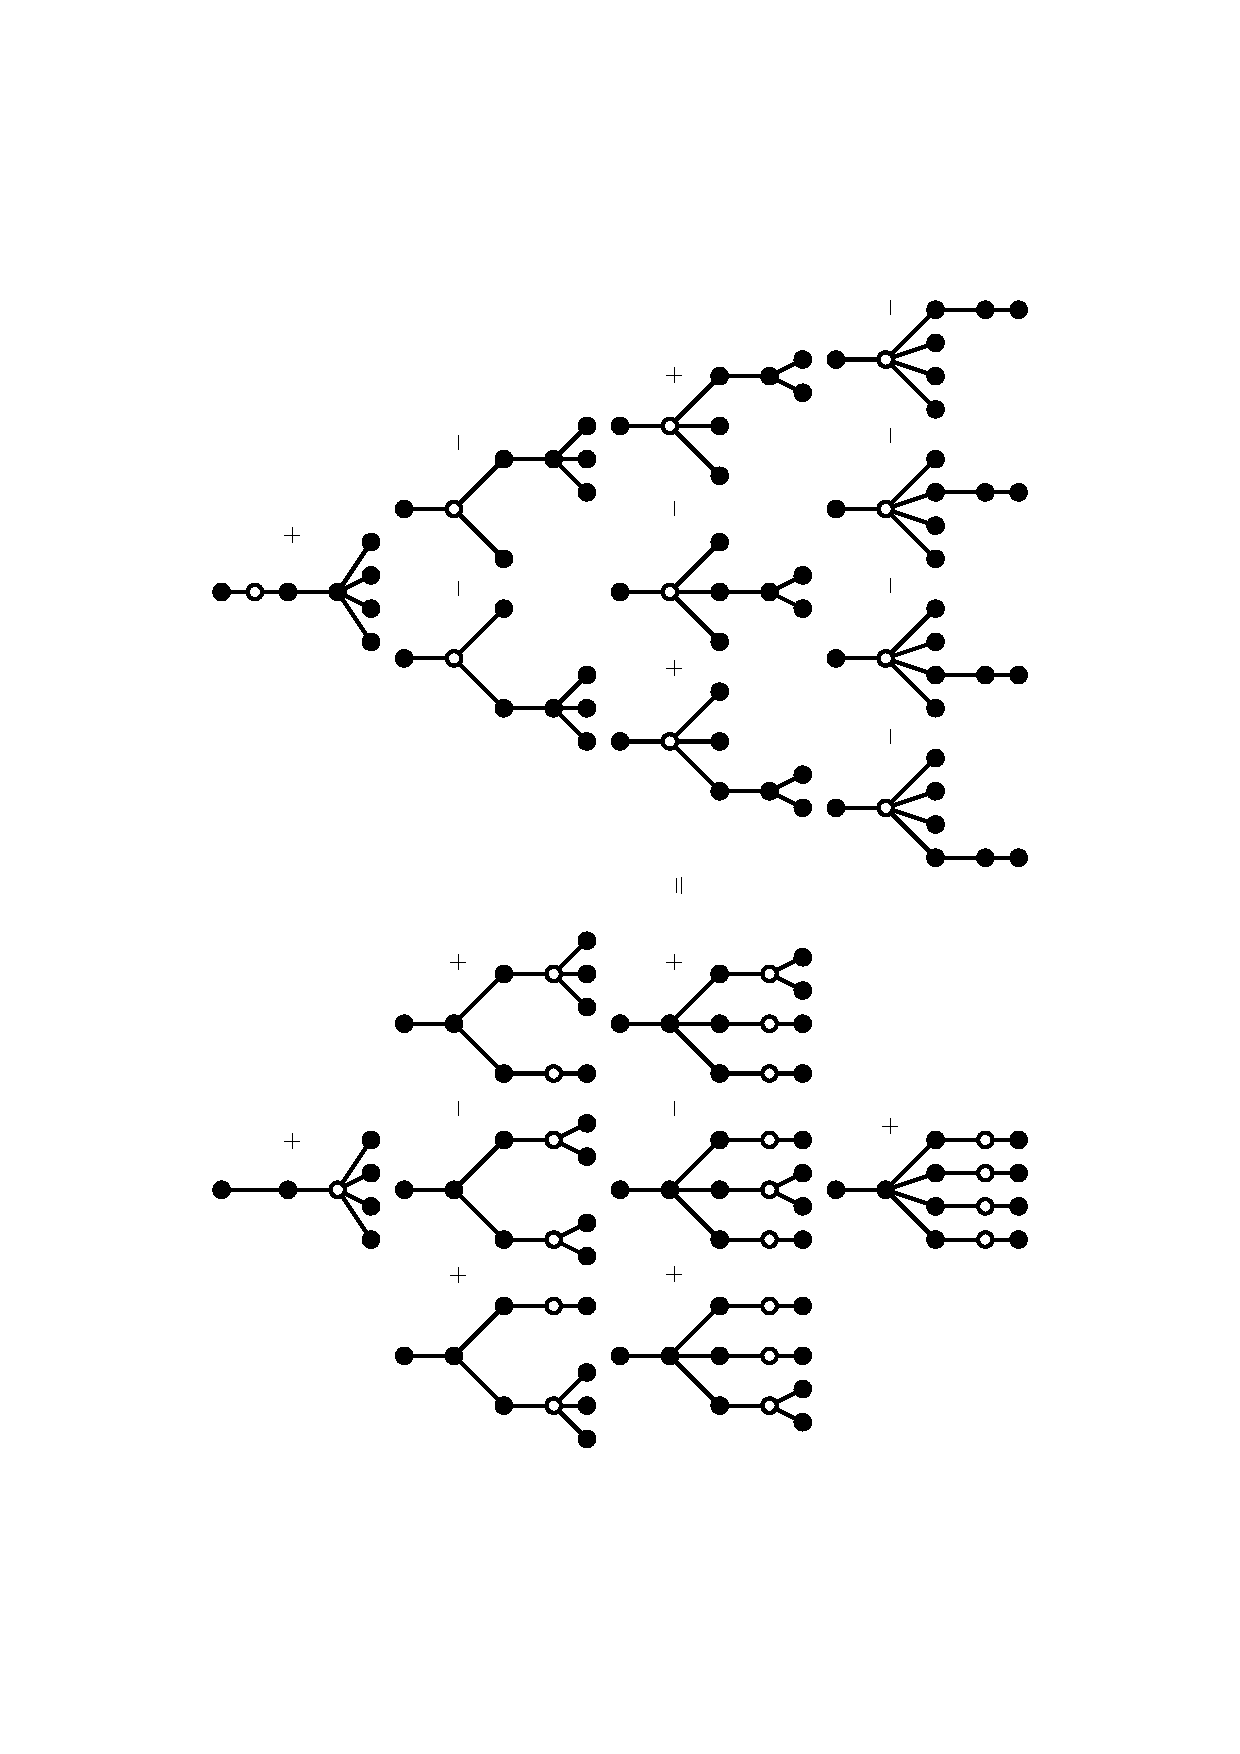
\includepdf[pages=-]{pdfs/coverart_master.pdf}

\subsubsection{Rooted trees for DG-morphisms}
As we did for the relations describing a DG-algebra, we now present the full relations describing a DG-morphism. Let $A$ and $B$ be two DG-algebras. We think of these as $\A$-algebras by letting $m_i =0$ for $i\geq 3$. A map $f\colon A\longrightarrow B$ can then be considered to be a morphism of $\A$-algebras, $\{f_i\}$ by letting $f_1 = f$ and $f_i = 0$ for all $i\geq 2$. Then we get that the relations describing a DG-morphism are the following:

% The first stasheff identity for DG-morphisms using trees



\begin{center}
\begin{tikzpicture}[x=0.75pt,y=0.75pt,yscale=-1,xscale=1]
%uncomment if require: \path (0,513); %set diagram left start at 0, and has height of 513

%Straight Lines [id:da9149295825374517] 
\draw [line width=1.5]    (50,120) -- (50,103.36) ;
\draw [shift={(50,100)}, rotate = 270] [color={rgb, 255:red, 0; green, 0; blue, 0 }  ][line width=1.5]      (0, 0) circle [x radius= 4.36, y radius= 4.36]   ;
\draw [shift={(50,120)}, rotate = 270] [color={rgb, 255:red, 0; green, 0; blue, 0 }  ][fill={rgb, 255:red, 0; green, 0; blue, 0 }  ][line width=1.5]      (0, 0) circle [x radius= 4.36, y radius= 4.36]   ;
%Straight Lines [id:da6451654153315307] 
\draw [line width=1.5]    (50,96.65) -- (50,80) ;
\draw [shift={(50,80)}, rotate = 270] [color={rgb, 255:red, 0; green, 0; blue, 0 }  ][fill={rgb, 255:red, 0; green, 0; blue, 0 }  ][line width=1.5]      (0, 0) circle [x radius= 4.36, y radius= 4.36]   ;
\draw [shift={(50,100)}, rotate = 270] [color={rgb, 255:red, 0; green, 0; blue, 0 }  ][line width=1.5]      (0, 0) circle [x radius= 4.36, y radius= 4.36]   ;
%Straight Lines [id:da951655139734809] 
\draw [line width=1.5]    (110,80) -- (110,63.36) ;
\draw [shift={(110,60)}, rotate = 270] [color={rgb, 255:red, 0; green, 0; blue, 0 }  ][line width=1.5]      (0, 0) circle [x radius= 4.36, y radius= 4.36]   ;
\draw [shift={(110,80)}, rotate = 270] [color={rgb, 255:red, 0; green, 0; blue, 0 }  ][fill={rgb, 255:red, 0; green, 0; blue, 0 }  ][line width=1.5]      (0, 0) circle [x radius= 4.36, y radius= 4.36]   ;
%Straight Lines [id:da5333607615257305] 
\draw [line width=1.5]    (110,56.65) -- (110,40) ;
\draw [shift={(110,40)}, rotate = 270] [color={rgb, 255:red, 0; green, 0; blue, 0 }  ][fill={rgb, 255:red, 0; green, 0; blue, 0 }  ][line width=1.5]      (0, 0) circle [x radius= 4.36, y radius= 4.36]   ;
\draw [shift={(110,60)}, rotate = 270] [color={rgb, 255:red, 0; green, 0; blue, 0 }  ][line width=1.5]      (0, 0) circle [x radius= 4.36, y radius= 4.36]   ;
%Straight Lines [id:da3030831638766034] 
\draw [line width=1.5]    (110,100) -- (110,80) ;
\draw [shift={(110,80)}, rotate = 270] [color={rgb, 255:red, 0; green, 0; blue, 0 }  ][fill={rgb, 255:red, 0; green, 0; blue, 0 }  ][line width=1.5]      (0, 0) circle [x radius= 4.36, y radius= 4.36]   ;
\draw [shift={(110,100)}, rotate = 270] [color={rgb, 255:red, 0; green, 0; blue, 0 }  ][fill={rgb, 255:red, 0; green, 0; blue, 0 }  ][line width=1.5]      (0, 0) circle [x radius= 4.36, y radius= 4.36]   ;
%Straight Lines [id:da32521299307207774] 
\draw [line width=1.5]    (110,120) -- (110,100) ;
\draw [shift={(110,100)}, rotate = 270] [color={rgb, 255:red, 0; green, 0; blue, 0 }  ][fill={rgb, 255:red, 0; green, 0; blue, 0 }  ][line width=1.5]      (0, 0) circle [x radius= 4.36, y radius= 4.36]   ;
\draw [shift={(110,120)}, rotate = 270] [color={rgb, 255:red, 0; green, 0; blue, 0 }  ][fill={rgb, 255:red, 0; green, 0; blue, 0 }  ][line width=1.5]      (0, 0) circle [x radius= 4.36, y radius= 4.36]   ;
%Straight Lines [id:da02196000233385731] 
\draw [line width=1.5]    (50,80) -- (50,60) ;
\draw [shift={(50,60)}, rotate = 270] [color={rgb, 255:red, 0; green, 0; blue, 0 }  ][fill={rgb, 255:red, 0; green, 0; blue, 0 }  ][line width=1.5]      (0, 0) circle [x radius= 4.36, y radius= 4.36]   ;
\draw [shift={(50,80)}, rotate = 270] [color={rgb, 255:red, 0; green, 0; blue, 0 }  ][fill={rgb, 255:red, 0; green, 0; blue, 0 }  ][line width=1.5]      (0, 0) circle [x radius= 4.36, y radius= 4.36]   ;
%Straight Lines [id:da16499633217703824] 
\draw [line width=1.5]    (50,60) -- (50,40) ;
\draw [shift={(50,40)}, rotate = 270] [color={rgb, 255:red, 0; green, 0; blue, 0 }  ][fill={rgb, 255:red, 0; green, 0; blue, 0 }  ][line width=1.5]      (0, 0) circle [x radius= 4.36, y radius= 4.36]   ;
\draw [shift={(50,60)}, rotate = 270] [color={rgb, 255:red, 0; green, 0; blue, 0 }  ][fill={rgb, 255:red, 0; green, 0; blue, 0 }  ][line width=1.5]      (0, 0) circle [x radius= 4.36, y radius= 4.36]   ;

% Text Node
\draw (68,70.4) node [anchor=north west][inner sep=0.75pt]    {$=$};
% Text Node
\draw (20,47.4) node [anchor=north west][inner sep=0.75pt]    {$d_{A}$};
% Text Node
\draw (120,91.4) node [anchor=north west][inner sep=0.75pt]    {$d_{B}$};
% Text Node
\draw (27,90.4) node [anchor=north west][inner sep=0.75pt]    {$f$};
% Text Node
\draw (119,50.4) node [anchor=north west][inner sep=0.75pt]    {$f$};


\end{tikzpicture}
\end{center}

and 


% The second stasheff identity for DG-morphisms using trees



\begin{center}
\begin{tikzpicture}[x=0.75pt,y=0.75pt,yscale=-1,xscale=1]
%uncomment if require: \path (0,513); %set diagram left start at 0, and has height of 513

%Straight Lines [id:da9654905799619733] 
\draw [line width=1.5]    (50,70) -- (30,50) ;
\draw [shift={(30,50)}, rotate = 225] [color={rgb, 255:red, 0; green, 0; blue, 0 }  ][fill={rgb, 255:red, 0; green, 0; blue, 0 }  ][line width=1.5]      (0, 0) circle [x radius= 4.36, y radius= 4.36]   ;
\draw [shift={(50,70)}, rotate = 225] [color={rgb, 255:red, 0; green, 0; blue, 0 }  ][fill={rgb, 255:red, 0; green, 0; blue, 0 }  ][line width=1.5]      (0, 0) circle [x radius= 4.36, y radius= 4.36]   ;
%Straight Lines [id:da12989711620017252] 
\draw [line width=1.5]    (50,90) -- (50,70) ;
\draw [shift={(50,70)}, rotate = 270] [color={rgb, 255:red, 0; green, 0; blue, 0 }  ][fill={rgb, 255:red, 0; green, 0; blue, 0 }  ][line width=1.5]      (0, 0) circle [x radius= 4.36, y radius= 4.36]   ;
\draw [shift={(50,90)}, rotate = 270] [color={rgb, 255:red, 0; green, 0; blue, 0 }  ][fill={rgb, 255:red, 0; green, 0; blue, 0 }  ][line width=1.5]      (0, 0) circle [x radius= 4.36, y radius= 4.36]   ;
%Straight Lines [id:da316004338934887] 
\draw [line width=1.5]    (50,70) -- (70,50) ;
\draw [shift={(70,50)}, rotate = 315] [color={rgb, 255:red, 0; green, 0; blue, 0 }  ][fill={rgb, 255:red, 0; green, 0; blue, 0 }  ][line width=1.5]      (0, 0) circle [x radius= 4.36, y radius= 4.36]   ;
\draw [shift={(50,70)}, rotate = 315] [color={rgb, 255:red, 0; green, 0; blue, 0 }  ][fill={rgb, 255:red, 0; green, 0; blue, 0 }  ][line width=1.5]      (0, 0) circle [x radius= 4.36, y radius= 4.36]   ;
%Straight Lines [id:da9149295825374517] 
\draw [line width=1.5]    (50,130) -- (50,113.36) ;
\draw [shift={(50,110)}, rotate = 270] [color={rgb, 255:red, 0; green, 0; blue, 0 }  ][line width=1.5]      (0, 0) circle [x radius= 4.36, y radius= 4.36]   ;
\draw [shift={(50,130)}, rotate = 270] [color={rgb, 255:red, 0; green, 0; blue, 0 }  ][fill={rgb, 255:red, 0; green, 0; blue, 0 }  ][line width=1.5]      (0, 0) circle [x radius= 4.36, y radius= 4.36]   ;
%Straight Lines [id:da6451654153315307] 
\draw [line width=1.5]    (50,106.65) -- (50,90) ;
\draw [shift={(50,90)}, rotate = 270] [color={rgb, 255:red, 0; green, 0; blue, 0 }  ][fill={rgb, 255:red, 0; green, 0; blue, 0 }  ][line width=1.5]      (0, 0) circle [x radius= 4.36, y radius= 4.36]   ;
\draw [shift={(50,110)}, rotate = 270] [color={rgb, 255:red, 0; green, 0; blue, 0 }  ][line width=1.5]      (0, 0) circle [x radius= 4.36, y radius= 4.36]   ;
%Straight Lines [id:da5757816173269195] 
\draw [line width=1.5]    (130,90) -- (130,73.36) ;
\draw [shift={(130,70)}, rotate = 270] [color={rgb, 255:red, 0; green, 0; blue, 0 }  ][line width=1.5]      (0, 0) circle [x radius= 4.36, y radius= 4.36]   ;
\draw [shift={(130,90)}, rotate = 270] [color={rgb, 255:red, 0; green, 0; blue, 0 }  ][fill={rgb, 255:red, 0; green, 0; blue, 0 }  ][line width=1.5]      (0, 0) circle [x radius= 4.36, y radius= 4.36]   ;
%Straight Lines [id:da3656762363310584] 
\draw [line width=1.5]    (130,66.65) -- (130,50) ;
\draw [shift={(130,50)}, rotate = 270] [color={rgb, 255:red, 0; green, 0; blue, 0 }  ][fill={rgb, 255:red, 0; green, 0; blue, 0 }  ][line width=1.5]      (0, 0) circle [x radius= 4.36, y radius= 4.36]   ;
\draw [shift={(130,70)}, rotate = 270] [color={rgb, 255:red, 0; green, 0; blue, 0 }  ][line width=1.5]      (0, 0) circle [x radius= 4.36, y radius= 4.36]   ;
%Straight Lines [id:da7746455127014982] 
\draw [line width=1.5]    (170,90) -- (170,73.36) ;
\draw [shift={(170,70)}, rotate = 270] [color={rgb, 255:red, 0; green, 0; blue, 0 }  ][line width=1.5]      (0, 0) circle [x radius= 4.36, y radius= 4.36]   ;
\draw [shift={(170,90)}, rotate = 270] [color={rgb, 255:red, 0; green, 0; blue, 0 }  ][fill={rgb, 255:red, 0; green, 0; blue, 0 }  ][line width=1.5]      (0, 0) circle [x radius= 4.36, y radius= 4.36]   ;
%Straight Lines [id:da06773749826026121] 
\draw [line width=1.5]    (170,66.65) -- (170,50) ;
\draw [shift={(170,50)}, rotate = 270] [color={rgb, 255:red, 0; green, 0; blue, 0 }  ][fill={rgb, 255:red, 0; green, 0; blue, 0 }  ][line width=1.5]      (0, 0) circle [x radius= 4.36, y radius= 4.36]   ;
\draw [shift={(170,70)}, rotate = 270] [color={rgb, 255:red, 0; green, 0; blue, 0 }  ][line width=1.5]      (0, 0) circle [x radius= 4.36, y radius= 4.36]   ;
%Straight Lines [id:da42664800881229814] 
\draw [line width=1.5]    (150,110) -- (130,90) ;
\draw [shift={(130,90)}, rotate = 225] [color={rgb, 255:red, 0; green, 0; blue, 0 }  ][fill={rgb, 255:red, 0; green, 0; blue, 0 }  ][line width=1.5]      (0, 0) circle [x radius= 4.36, y radius= 4.36]   ;
\draw [shift={(150,110)}, rotate = 225] [color={rgb, 255:red, 0; green, 0; blue, 0 }  ][fill={rgb, 255:red, 0; green, 0; blue, 0 }  ][line width=1.5]      (0, 0) circle [x radius= 4.36, y radius= 4.36]   ;
%Straight Lines [id:da6893790318561632] 
\draw [line width=1.5]    (150,130) -- (150,110) ;
\draw [shift={(150,110)}, rotate = 270] [color={rgb, 255:red, 0; green, 0; blue, 0 }  ][fill={rgb, 255:red, 0; green, 0; blue, 0 }  ][line width=1.5]      (0, 0) circle [x radius= 4.36, y radius= 4.36]   ;
\draw [shift={(150,130)}, rotate = 270] [color={rgb, 255:red, 0; green, 0; blue, 0 }  ][fill={rgb, 255:red, 0; green, 0; blue, 0 }  ][line width=1.5]      (0, 0) circle [x radius= 4.36, y radius= 4.36]   ;
%Straight Lines [id:da7344463324537529] 
\draw [line width=1.5]    (150,110) -- (170,90) ;
\draw [shift={(170,90)}, rotate = 315] [color={rgb, 255:red, 0; green, 0; blue, 0 }  ][fill={rgb, 255:red, 0; green, 0; blue, 0 }  ][line width=1.5]      (0, 0) circle [x radius= 4.36, y radius= 4.36]   ;
\draw [shift={(150,110)}, rotate = 315] [color={rgb, 255:red, 0; green, 0; blue, 0 }  ][fill={rgb, 255:red, 0; green, 0; blue, 0 }  ][line width=1.5]      (0, 0) circle [x radius= 4.36, y radius= 4.36]   ;

% Text Node
\draw (86,82.4) node [anchor=north west][inner sep=0.75pt]    {$=$};


\end{tikzpicture}    
\end{center}

All other relations will include some copy of $m_i$ for $i\geq 3$ or $f_j$ for $j\geq 2$. Hence these two relations are the only two ones we get for a DG-morphism. We also have some degree preservation requirements, but these hold because $f=f_1$ is a degree $0$ map, meaning it preserves homogeneous degrees of elements. 






\section{Kadeishvili's theorem}

One of the main reasons we introduce these $\A$-algebras, instead of just working directly with DG-algebras, is because of a theorem proved by Kadeishvili in \cite{kadeishvili}. We have seen that not all DG-algebras have a quasi-isomorphism to their cohomology algebra---as not all DG-algebras are formal---but this theorem will allow us to sort of approximate the existence of such a morphism. The caveat is that DG-algebras no longer suffice, and we must venture into the world of $\A$-algebras. The idea is to build an $\A$-structure on the cohomology algebra of a DG-algebra, such that instead of a DG-quasi-isomorphism we have an $\A$-quasi-isomorphism connecting them. 

We then want to study these more complicated structures and morphisms in order to figure out if they collapse to our more simple DG-algebra world in certain situations. If we can do and understand this, it will give us a new tool to figure out if a DG-algebra is formal. So far our tool for checking formality of a DG-algebra---namely the Massey products---have been a sort of non-criteria. By this we means that we can use them to easily spot whether a DG-algebra is non-formal, but we can not use them to check formality. This more general theory will allow us to create a more ``perfect'' version of Massey products in order to actually prove that a class of DG-algebras are formal. 

\begin{definition}[Minimal $\A$-algebra]
\index{Minimal $\A$-algebra}
\label{def:minimal_A_infinity-algebra}
We say an $\A$-algebra $(A, m)$ is minimal if we have $m_1 = 0$. 
\end{definition}

\begin{theorem}[Kadeishvili's theorem]
\label{thm:Kadeishvilis_theorem}
\index{Kadeishvili's theorem}
Let $(A,d)$ be a DG-algebra. Then there exists a minimal $\A$-algebra structure on its cohomology algebra $H(A)$, and a quasi-isomorphism of $\A$-algebras\index{$\A$-quasi-isomorphism} $H(A)\rightsquigarrow A$. 
\end{theorem}

Before we look into the proof, we discuss the strategy and some implications it would have. The theorem is important for us, as---as we have seen---not all DG-algebras have a quasi-isomorphism to their cohomology, or even a zig-zag of quasi-isomorphisms. We have also seen that taking the cohomology of a DG-algebra kills the homotopical information. We saw this implicitly through the Massey products all being vanishing in a DG-algebra with trivial differential. This theorem would allow us to kill off the homotopy information---by taking cohomology---but still preserve the quasi-isomorphism type. We will see why this is important for us in the next section, when we look at formality through the lens of Kadeishvilis theorem.

For the strategy, we have already seen---at least the beginnings of---how to construct an $\A$-structure from a deformation retraction\index{Deformation retraction} between a DG-algebra and a chain complex. This is also the idea for this theorem. We construct a particular deformation retract, and use the earlier discussed procedure to produce both the $\A$-structure and the $\A$-quasi-isomorphism that we want. We remind the reader that we are working over a field $k$, so the graded components of the objects are vector spaces, which makes it easy to construct compliments and direct sums. The following construction is due to Lu, Palmieri, Wu and Zhang in \cite{Ext} as a special case of the more general approach by Merkulov in \cite{Merkulov}. 

The deformation retraction $(A, H(A), i, p, h)$ we are going to use is the following. Decompose $A$ into $Z\oplus H\oplus L$, where $Z=\ker d$, $H\cong H(A)$ and $L\cong B[+1]$. Because of this particular $H$, we use this in our deformation retraction, instead of $H(A)$. The map $i$ is the inclusion of $H$ into $A$, $p$ the projection and $h$ the map given by the matrix 
\begin{equation*}
h^n = 
\begin{bmatrix}
0 & 0 & (d_{LB}^{n-1})^{-1}\\
0 & 0 & 0\\
0 & 0 & 0
\end{bmatrix}, 
\end{equation*}
where $d_{LB}$ comes from the description of $d$ as a matrix as follows:
\begin{equation*}
d^n = 
\begin{bmatrix}
    d^n_{BB} & d^n_{BH} & d^n_{BL} \\
    d^n_{HB} & d^n_{HH} & d^n_{HL} \\
    d^n_{LB} & d^n_{LH} & d^n_{LL} 
\end{bmatrix}
\colon B^n\oplus H^n\oplus L^n \longrightarrow B^{n+1}\oplus H^{n+1}\oplus L^{n+1}
\end{equation*}

A more detailed construction---and the proof of this actually being a deformation retraction---is moved to appendix A. 

Note that this deformation retraction is not unique, as it requires making choices for the subspaces $H^n$ and $L^n$. Thus we can get many different such deformation retractions by altering these choices. In the theorem we want to prove, namely that such a deformation retraction gives us an $\A$-structure on the cohomology algebra, we will get different, albeit $\A$-quasi-isomorphic $\A$-structures when we alter the choices of the subspaces. Since we are only interested in an $\A$-structure on $H(A)$ such that it is $\A$-quasi-isomorphic to $A$, these choices of subspaces are not important---as we have our desired $\A$-quasi-isomorphism regardless. This is because we are not really interested in the structure itself, merely its existence, and its relation to formality. 

We now restate Kadeishvili's theorem in this new situation we have created.

\begin{theorem}[Kadeishvili's theorem]
\label{thm:Kadeishvilis_theorem2}
\index{Kadeishvili's theorem}
Let $(A, m, d)$ be a DG-algebra, $H(A)$ its cohomology algebra and $(A, H(A), p, i, h)$ be the deformation retraction described above. Then there is a minimal $\A$-structure $\{m_n\}$ on $H(A)$ and an $\A$-quasi-isomorphism $I\colon H(A)\rightsquigarrow A$ that extends $i$. 
\end{theorem}
\begin{proof}
We let $m_1=0$, $I_1=i$ and $h\lambda_1 = -id_A$. Then for $n\geq 2$ we recursively define
\begin{equation*}
    \lambda_n = \sum_{k=1}^{n-1}(-1)^{k+1}m(h\lambda_k\otimes h\lambda_{n-k})
\end{equation*}
Then our $\A$-structure and $\A$-quasi-isomorphism is given by 
\begin{align*}
    m_n &= p\circ \lambda_n \\
    I_n &= h\circ \lambda_n
\end{align*}
\end{proof}

We call such a minimal $\A$-structure on the cohomology algebra $H(A)$---coming from a deformation retraction of the type above---a \emph{Merkulov model}\index{Merkulov model} of $A$. 

We will not prove that these do in fact satisfy the Stasheff identities, but we refer the reader to \cite{kadeishvili} for the original, and much more general proof. We do however write out what happens for some low $n$. 

% \begin{proof}
% Recall that the deformation retraction comes from a splitting $A=B\oplus H\oplus L$, where $B^n = \ima d^{n-1}$ and $H\cong H(A)$. For any $b\in B$ there is a unique $l\in L$ such that $b = d(l)$. We then define a map $Q\colon B\longrightarrow L$ such that $Q(b)=l$. We then get that $Qd = id_B$ and $dQ = id_L$.

% For any $[a] \in H(A)$ there is a unique $a_0\in H$, representing the cohomology class $[a]$. We define $I_1([a])=a_0$ and $I_2 = Q(I_1 m_2 - m(I_1\otimes I_1))$, where $m$ is the product in $A$, and $m_2$ is the induced product in $H(A)$. Here on we use an inductive argument. Suppose that $m_j$ and $I_j$ have been defined for $1< k$. 

% Let $F_k$ be the map defined by 
% \begin{equation*}
%     F_k = \sum_{i+j = k}(-1)^{i-1}m(I_i\otimes I_j) - \sum_{r+s+t=k}(-1)^{r+st}I_{r+1+t}(id^{\otimes r}\otimes m_s\otimes id^{\otimes t}).
% \end{equation*}
% Notice that it only uses already defined $I_i$'s and $m_i$'s, so it is in fact a well defined map. 

% The relation we need then becomes 
% \begin{equation*}
%     d I_k = I_1 m_k - F_k.
% \end{equation*}
% As we have that $\partial F_k = 0$ we know that every time we use it on an element $x_1\otimes \cdots \otimes x_k \in H(A)^{\otimes k}$ we get a cocycle in $A$. We then define $m_k$ to be the map that takes in such an element $x_1\otimes \cdots \otimes x_k$ and returns the cohomology class of the cycle that $F_k$ produces. More simply we can write that $m_k = \overline{F_k}$, i.e. the induced map on cohomology. Since $I_1$ chooses cocycles for the cohomology classes we get that $I_1m_k-F_k$ is cohomologous to zero. For some free generators $x_i \in H(A)$ we can then define $I_k$ to be a map that sends the product of such free generators $x_1\otimes \cdots \otimes x_k$ to a cocycle bounding $(I_1 m_k-F_k)(x_1\otimes \cdots \otimes x_k)$. The whole map is defined by extending this linearly. 

% %We then define $m_k$ and $I_k$ from the relations $I_1 m_k - d I_k = F_k$ and $I_k = Q(I_1 m_k - F_k)$. 
% \end{proof}
% \todo[inline]{Can we check the relevant calculations to check that this in fact gives an $\A$-structure?}

For $n=2$ we get
\begin{equation*}
    m_2 = p\circ \lambda_2 = p(m(h\lambda_1)\otimes h\lambda_1) = p(m(-id_A\otimes -id_A) = pm
\end{equation*}

which is just the induced multiplication from $A$ on $H(A)$. Earlier when we looked at transferring algebraic structures, we also used the map $i$ to describe the induced operation, but here we omit it, as we think of $H^i$ as a subspace of $A^i$. For $n=3$ we get 
\begin{align*}
    m_3 
    &= p\circ \lambda_3 \\
    &= p(m(h\lambda_1\otimes h\lambda_2)-m(h\lambda_2\otimes h\lambda_1)) \\
    &= p(m((-id_A)\otimes hm)-m(hm\otimes (-id_A))) \\
    &= p(m(hm\otimes id_A)-m(id_A\otimes hm))
\end{align*}
which we should recognize as the same $m_3$ we constructed from the general deformation retraction we studied earlier in \cref{ch:3}, namely the associating homotopy\index{Associating homotopy} between $m_2(id\otimes m_2)$ and $m_2(m_2\otimes id)$. Since $m_2$ is just the induced product on $H$, we actually know that it is associative, i.e. $m_2(id\otimes m_2)-m_2(m_2\otimes id)=0$, as it is isomorphic to $H(A)$, which is an associative DG-algebra. If we look at the $n=3$ equation defining an $\A$-algebra we have 
\begin{equation*}
    m_2(id\otimes m_2)-m_2(m_2\otimes id) = m_1 m_3 + m_3(m_1\otimes id\otimes id + id\otimes m_1\otimes id + id\otimes id \otimes m_1), 
\end{equation*}
but, as we have $m_1=0$, we are totally fine with having an associative product in this scenario! This means that we have $\partial m_3 = 0$, i.e. that it is a cocycle in $Hom(A^{\otimes 3}, A)$. This, however, does not mean it zero itself.

We mentioned earlier that an alternative way of describing the Stasheff identities\index{The Stasheff identities} was given by 
\begin{equation*}
    \partial m_n = - \sum_{r+s+t=n}(-1)^{r+st}m_{r+s+t}(id^{\otimes r}\otimes m_s\otimes id^{\otimes t})
\end{equation*}
where $r,s,t\geq 1$ and $\partial m_n = m_1m_n - (-1)^{|m_n|}m_n\left(\sum_{r=0}^{n-1}(id^{\otimes r}\otimes m_1\otimes id^{\otimes n-r-1})\right)$. Since all of the terms in $\partial m_n$ contain a copy of $m_1$, we know that the entire sum will be zero, i.e. $\partial m_n = 0$, meaning that all the higher operations are cocycles in their respective cochain complexes $Hom(A^{\otimes n}, A)$. Hence the Stasheff identities for the $\A$-structure we get from Kadeishvili's theorem are
\begin{equation*}
    \sum_{r+s+t=n}(-1)^{r+st}m_{r+s+t}(id^{\otimes r}\otimes m_s\otimes id^{\otimes t}) = 0
\end{equation*}
for $r, s, t\geq 1$. We earlier formed an upside down triangle of trees representing these Stasheff identities. If we remove the top and bottom row of this triangle we are left with the relation just described. Notice that this new truncated upside down triangle contains 
\begin{equation*}
    \left(\sum_{i=1}^n i\right) - n-1 = \left(\sum_{i=1}^{n-1} i\right) -1
\end{equation*}
trees, i.e. one less than the $n-1$'st triangle number. This is not by coincidence equal to the number of facets in $K(n+1)$, the $n+1$'st Stasheff associahedron\index{Stasheff associahedron}. 



\begin{remark}
There are several generalizations of Kadeishvili's theorem. Kadeishvili's original proof holds over general commutative rings, if one requires that the cohomology algebra $H(A)$ is a projective module over $A$. This result was extended in \cite{Sagave} to hold for any commutative ring, without any assumptions for $H(A)$---if one instead of a minimal $\A$-algebra uses so-called minimal derived $\A$-algebra. The theorem was later shown to hold if $A$ is an $\A$-algebra instead of just a DG-algebra. See \cite{transfer} for explicit formulas and proofs. This means that the transfer of an $\A$-algebra through a deformation retraction, is again an $\A$-algebra.

The results have also been generalized to the theory of $\infty$-operads, where such a transfer is possible for several other types of algebras, notably DG-Lie-algebras. Most of these results are contained in \cite{operads}. Note that in these other settings the theorem is often referred to as ``the homotopy transfer theorem'' or the ``minimal models theorem''. 
\end{remark}






\subsection{Connection to formality}

Now that we have this more general approach to studying the relationship between a DG-algebra and its cohomology algebra, we need to know how it relates back to our original interests---namely formality. Recall that by \cref{thm:span}, $A$ being a formal DG-algebra\index{Formal DG-algebra} means that we have a span of DG-quasi-isomorphisms between $A$ and $H(A)$, i.e. $H(A)\longleftarrow M\longrightarrow A$. By Kadeishvili's theorem we now have more than a DG-structure on $H(A)$, as we have in fact an $\A$-structure $\{m_n\}$, but we also have a direct $\A$-quasi-isomorphism $q\colon H(A)\rightsquigarrow A$. We know that if $m_n = 0$ for $n\geq 3$ then $H(A)$ is in fact a DG-algebra, so we can think of these possibly non-trivial $m_n$'s as measuring how far away $A$ is from being formal. This is of course informal, but it will soon turn out to also be a precise statement. 

One of the other main reasons for passing to $\A$-algebras is that their homotopy theory is better behaved than for DG-algebras. We have in fact already seen this, as a deformation retraction\index{Deformation retraction} of a DG-algebra is not necessarily a DG-algebra, but by the generalizaton of Kadeishvili's theorem we mentioned, this property in fact holds for $\A$-algebras. This means that being an $\A$-algebra is a ``homotopy stable'' property. 

We have also seen that DG-quasi-isomorphisms are not the nicest ones, as they are not homotopy invertible. This is because not all isomorphisms in the homotopy category\index{The homotopy category} $hoDGA_k$ comes from a DG-quasi-isomorphism in $DGA_k$. This resulted is us having to use zig-zags and spans of DG-quasi-isomorphisms instead of just direct ones. This property is luckily also fixed by passing to $\A$-algebras, meaning that all $\A$-quasi-isomorphisms are $\A$-homotopy equivalences. 


\begin{definition}[$\A$-homotopy]
\label{def:A_infinity-homotopy}
\index{$\A$-homotopy}
Let $(A, m^A)$ and $(B, m^B)$ be $\A$-algebras. Two $\A$-morphisms $\{f_n\}, \{g_n\}$ between them are called homotopic if there exists a family of graded homogeneous multilinear degree $-1$ maps $h_n:A^{\otimes n}\longrightarrow B$, such that the difference $g_n-f_n$ is equal to
\begin{equation*}
\sum_{i_1+\cdots i_r = n}m^B_{r+1+t} (g_{i_1}\otimes \cdots \otimes g_{i_t}\otimes h_s \otimes f_{i_{t+1}}\otimes \cdots \otimes f_{i_r} ) + \sum_{r+s+t = n}h_{r+1+t} (id^{\otimes r}\otimes m^A_s \otimes id^{\otimes t})
\end{equation*}
where $r, t\geq 0, n, s\geq 1$ as usual. 
\end{definition}


\begin{proposition}
\label{prop:infty-qi_homotopy_invertible}
Let $(A, m^A)$ and $(B, m^B)$ be $\A$-algebras and $q:A\rightsquigarrow B$ an $\A$-quasi-isomorphism. Then there exists an $\A$-quasi-isomorphism $q':B\rightsquigarrow A$ that is a $\A$-homotopy inverse of $f$. This means that the class of $\A$-quasi-isomorphisms is the same as the class of $\A$-homotopy equivalences. 
\end{proposition}

We wont prove this result, as the proof uses some machinery that we will not cover in this thesis. More precisely one at least needs the bar and cobar constructions for $\A$-algebras. The reader interested in the proof is referred to \cite[Corollary 1.3.1.3]{french1}. 

The next step is to figure out how an $\A$-quasi-isomorphism relates to a DG-quasi-isomorphism. This is done through the following result.

\begin{corollary}
\label{cor:zigzag-quasi}
Two DG-algebras $(A, d_A)$ and $(B, d_B)$ is connected by a zig-zag of DG-quasi-isomorphisms
\begin{equation*}
    A \overset{\sim}\longleftarrow \bullet \overset{\sim}\longrightarrow \cdots \overset{\sim}\longleftarrow \bullet \overset{\sim}\longrightarrow B, 
\end{equation*}
i.e. they are quasi-isomorphic, if and only if there is an $\A$-quasi-isomorphism $A\rightsquigarrow B$. 
\end{corollary}

\begin{proof}
Assume we have a zig-zag of DG-quasi-isomorphisms between $A$ and $B$. Recall that by \cref{thm:span} we can reduce the zig-zag to a single span of DG-quasi-isomorphisms $A\overset{q}\longleftarrow C\overset{p}\longrightarrow B$. We now interpret $A$, $B$ and $C$ as $\A$-algebras, and $q, p$ as morphisms of $\A$ algebras. This is the same standard procedure we have described before, i.e. letting $m^A_n = m^B_n = m^C_n = 0$ for all $n\geq 3$ and defining $\{q_n\}$ by $q_1 = q$ and $q_m = 0$ for $m\geq 2$ and similarly for $p$. By abuse of notation we denote these $\A$-morphisms again by $q$ and $p$. Notice that since $q$ and $p$ are DG-quasi-isomorphisms, then $q$ and $p$ are $\A$-quasi-isomorphisms as well. We then have a span 
\begin{center}
\begin{tikzpicture}
\node (1) {$A$};
\node (2) [node distance=1.3cm, right of=1] {$C$};
\node (3) [node distance=1.3cm, right of=2] {$B$};

\draw [-to, snake it] (2) to node {} (1);
\draw [-to, snake it] (2) to node {} (3); 
\end{tikzpicture}
\end{center}
of $\A$-quasi-isomorphisms. By \cref{prop:infty-qi_homotopy_invertible} we know these are invertible up to homotopy, hence we have an $\A$-quasi-isomorphism $q'\colon A\rightsquigarrow C$ such that $q\circ q' \sim id_A$ and $q'\circ q \sim id_C$. 

Since composition of two $DG$-quasi-isomorphisms is again a DG-quasi-isomorphism we know that this is the case for composition of $\A$-quasi-isomorphisms as well, as it only depends on the arity $1$ map. Thus $q'\circ p$ is an $\A$-quasi-isomorphism from $A$ to $B$. Notice that this can no longer have $(q'\circ p)_m = 0$ for $m\geq 2$ in general, as that would contradict DG-quasi-isomorphism being homotopy invertible. 

The other direction also holds, but to construct the zig-zag from a $\A$-quasi-isomorphism we again need the previously mentioned bar and cobar construction. To outline the idea, we can produce a DG-algebra $U(A)$ through the bar and cobar construction from an $\A$-algebra $A$. This can be though of as an ``anti Merkulov model''. This DG-algebra is universal, in the sense that any $\A$-morphism from $A$ to a DG-algebra $B$ factorizes uniquely through $U(A)$. Moreover $U(A)$ is $\A$-quasi-isomorphic to $A$. It can then be shown that if $A$ is a DG-algebra, then the map $U(A)\longrightarrow A$ is a DG-quasi-isomorphism. 

In our case we have two DG-algebras $A$ and $B$ and a $\A$-quasi-isomorphism $q\colon A\rightsquigarrow B$. We then get a zig-zag
\begin{equation*}
    A\overset{q_A}\longleftarrow U(A) \overset{U(q)}\longrightarrow U(B)\overset{q_B}\longrightarrow B
\end{equation*}
where $U(q)$ is a DG-quasi-isomorphism when $q$ is an $\A$-quasi-isomorphism. Hence we have our wanted zig-zag of DG-quasi-isomorphisms. 
\end{proof}

This tells us that $\A$-algebras are a generalization of DG-algebras, but not a too general one. In particular, we get that the homotopy category of DG-algebras is equivalent to the homotopy category of $\A$-algebras, as inverting quasi-isomorphisms produces the same isomorphism classes of objects by the above result, i.e. 
\begin{equation*}
	HoDGA_k \simeq Ho\infty Alg_k
\end{equation*}
Note that we have not discussed---an will not discuss---the model category of $\A$-algebras. 

As we have previously described formal DG-algebras in terms of the homotopy category $HoDGA_k$, we can now characterize them by using $\A$-algebras and $\A$-quasi-isomorphisms instead. 

\begin{corollary}
\label{cor:formal_A_infinity-qi}
Let $(A, d_A)$ be a DG-algebra and $H(A)$ its cohomology algebra, treated as a DG-algebra with trivial differential. Then $A$ is formal\index{Formal DG-algebra} if and only if there is an $\A$-quasi-isomorphism $q\colon H(A)\rightsquigarrow A$. 
\end{corollary}

Notice here that this is not the same statement as Kadeishvili's theorem, as here $H(A)$ is purely a DG-algebra, and not endowed with an $\A$-structure. We can however restate the corollary in more similar terms to Kadeishvili's theorem, then saying that a DG-algebra is formal if and only if its Merkulov model\index{Merkulov model} is again a DG-algebra, i.e. it has $m_i=0$ for all $i\geq 3$. 






\section{Uniform vanishing}




If we take a DG-algebra $A$, we know that it has a Merkulov model $H(A)\longrightarrow A$. Earlier we interpreted the map $m_3$ as an associating homotopy, but now we have $m_1 = 0$, as $H(A)$ is minimal. This makes the induced product $m_2$ an associative product, so how do we now interpret $m_3$? and $m_n$ in general? In chapter 2 we introduced some higher arity maps, $H(A)^{\otimes n}\longrightarrow H(A)$---namely the Massey products. It would be really nice if we could interpret $m_n$ as these already established products. This interpretation turns out to be faulty---explained a bit later---but as we are interested in formality, we need these to vanish anyway, so can we say something about this interpretation in the case where all the Massey products are vanishing? or when all the higher operations in the Merkulov model are trivial?

In \cite{DGMS} it is stated that formality is implied if the Massey products vanish ``uniformly''. It is mentioned as a remark to \cite[Theorem 4.1.]{DGMS}, where they prove that a DG-algebra admits a certain decomposition, if and only if it is formal. The authors say this is stronger that the Massey products vanishing normally. 

%The results stated in \cite{DGMS} are the following. 

%\begin{lemma}
%Any minimal dg algebra is isomorphic as an algebra to 
%$P[V_2\otimes V_4\otimes \cdots]\otimes \Lambda[V_1\otimes V_3 \otimes \cdots]$, where each of the vector spaces $V_i$ only have elements in degree $i$. In each of the $V_i$'s there is a subspace $C_i$ of the closed elements.
%\end{lemma}

%\begin{theorem}{\cite{DGMS}, Theorem 4.1.}
%A minimal dg algebra $A$ is formal if and only if there in each $V_i$ as defined above is a complement $N_i$ to $C_i$, i.e. such that $V_i=C_i\oplus N_i$, such that for any closed form $a$ in the ideal $I(\oplus N_i)$ is exact. Choosing such subspaces $N_i$ for all $i$ is equivalent to choosing a map $A\rightarrow H^*(A)$ inducing the identity on cohomology.
%\end{theorem}

%We have not covered minimal DG-algebras and minimal models of topological spaces, so we leave the proof of these out of the thesis. But 

This notion of uniform vanishing is interesting, so we try to look into what this could mean for the $\A$-structure on $H(A)$ of a DG-algebra $A$. We start by examining the connection between the higher products on $H(A)$ and Massey products. 

Recall from Kadeishvili's theorem that the cohomology algebra of a DG algebra has a natural $\A$-algebra structure which we call its Merkulov model if it is induced by a certain deformation retraction.

\begin{lemma}
Let $(A, m)$ be a DG algebra and $(H(A), \{m_n\})$ be a Merkulov model. Let further $x_1, x_2, x_3 \in H(A)$ such that $m_2(x_1\otimes x_2) = 0 = m_2(x_2\otimes x_3)$, then $m_3(x_1 \otimes x_2 \otimes x_3) \in \langle x_1, x_2, x_3 \rangle$, the Massey 3-product of $x_1, x_2$ and $x_3$.  
\end{lemma}
\begin{proof}
As $m_2(x_1 \otimes x_2) = 0$ we know that there exists some $a_{0,2}$ such that $d(a_{0,2}) = m(a_{0,1}, a_{1,2})$ where $a_{i-1, i}$ is a cocycle representing $x_i$. We choose this cocycle with some care by letting $\overline{a_{0,2}} = h(m(a_{0,1}, a_{1,2}))$. Almost in the same way, we choose for $m_2(x_2, x_3)$ the cocycle $a_{1,3} = h(m(a_{1,2}, a_{2,3}))$ In this way we have
\begin{align*}
    m_3(x_1\otimes x_2\otimes x_3) 
    &= p(m(hm(i, i), i)-m(i, hm(i,i))(x_1, x_2, x_3) \\
    &= p(m(hm(a_{0,1}, a_{1,2}), a_{2,3}) - (-1)^{|x_1|+1} m(a_{0,1}, hm(a_{1,2}, a_{2,3})) \\
    &= p(m(\overline{a_{0,2}}, a_{2,3})-m(\overline{a_{0,1}}, a_{1,3}))
\end{align*}
which we see is exactly the cohomology class of a representative of the Massey 3-product of $x_1, x_2, x_3$. Note that we have used the Koszul grading convention to get the correct signs. 
\end{proof}

This looks promising. It looks like some type of similarity between DG-algebras with Massey products and $\A$-structure on the cohomology algebra. This also provides us with examples of $\A$-algebras that are not just DG-algebras. We can for example consider the DG-algebra $k[x_1, x_2, x_3, a, b]$ that we had in chapter 2. If we define $m_3(x_1, x_2, x_3)=[\overline{a}x_1 + \overline{x_3}b]$, and the other combinations to be trivial, then we have an $\A$-algebra.

It was long thought to be a folklore truth that these higher order products in the $\A$-structure in fact gave representatives for the Massey products. This was then proven in \cite{Ext}, but later showed to have a gap in its argument in \cite{detection}. There are certain ways to make the higher products give representatives for the Massey products, but one requires stronger assumptions on the defining systems, which does not hold in general. These stronger assumptions are also developed in \cite{detection}. 

\begin{remark}
The observant reader might suspect something weird going on here. We earlier remarked that when we have two DG-algebras $A, B$ and an $\A$-quasi-isomorphism $q$ between them, then we have an informal equality between the Massey products, i.e 
\begin{equation*}
	q^*(\langle x_1, \ldots, x_n\rangle ) = \langle q^*(x_1),\ldots, q^*(x_n)\rangle .
\end{equation*}
But now we have an $\A$-quasi-isomorhism $H(A)\longrightarrow A$, and we have already proved that $H(A)$ only has vanishing Massey products. So does this mean that all DG-algebras have only vanishing Massey products? No. When $H(A)$ is not purely a DG-algebra, i.e. there is some $k\geq 3$ such that $m_k\neq 0$, then we need to take some more information into account in order to have such a correlation. We could do this by introducing Massey products on $\A$-algebras, which are more general than Massey products for DG-algebras. These were introduced by Stasheff in \cite{h-spaces}, and later used in \cite{infty-massey} to prove that the higher products on $H(A)$ do in fact form representatives of the Massey products on an $\A$-algebra $A$.
\end{remark}

As mentioned, we do not have a correspondence between the higher products and the Massey products, but we can still try to connect these higher products to formality. We actually have the following result---stating in a certain sense that if the higher products on the Merkulov model are uniformely trivial---then the DG-algebra is formal. This also provides us with the first general answer to our central question.

\begin{theorem}
Let $(A, d_A)$ be a DG-algebra and let $(H(A), m_n)$ be it's Merkulov model. If all the higher products are trivial, i.e. $m_i = 0$ for $i\geq 3$, then $A$ is formal. 
\end{theorem}
\label{thm:formal_iff_no_infty_massey}
\begin{proof}
As $H(A)$ is a Merkulov model, there is a quasi isomorphism of $\A$-algebras $q:H(A)\longrightarrow A$. Since all the higher products vanish we know that $H(A)$ is a DG algebra. This means that $A$ is formal by \cref{cor:formal}. 
\end{proof}

This resolves \textbf{Theorem C.} from the motivation earlier. As mentioned above, we can also finally answer the central question of the thesis. 
\begin{central}
Given a DG-algebra $A$, when do I know that $A$ is formal?
\end{central}

\textbf{Answer:} When the induced $\A$-structure $\{m_i\}$ on $H(A)$ has $m_i=0$ for $n\geq 3$, i.e. it has a Merkulov model which is a DG-algebra.  

The above result does not really rely on which $\A$-structure we have on $H(A)$. It can be shown that the least integer $k$ such that $m_k \neq 0$ is an invariant of all $\A$-structures on $H(A)$ that comes from a deformation retraction. This means that the above results holds regardless of which such $\A$-structure we might have. This result can also be proven using Hochschild cohomology, see for example \cite[Theorem 3.3.]{berglund}.

Even though we have answered the central question, it is important to explore what happens in the near vicinity of the solution. We can for example wonder what happens if not all of the higher products are trivial, but only some of them are. This situation is covered in \cite{detection} by the following two results.

\begin{theorem}[Theorem 2.1. in \cite{detection}]
Let $A$ be a DG-algebra and $x\in \langle x_1, \ldots, x_n\rangle$ with $n\geq 3$. Then for any $\A$ structure on $H(A)$ we have 
\begin{equation*}
    \epsilon m_n(x_1, \ldots, x_n) = x+\Gamma 
\end{equation*}
where $\Gamma \in \sum_{j=1}^{n-1}Im(m_j)$ and $\epsilon = (-1)^{\sum_{j=1}^{n-1} (n-j)|x_j|}$. 
\end{theorem}
\label{thm:infty_massey_recovers_massey}

\begin{corollary}[Corollary 2.2. in \cite{detection}]
Let $A$ be a DG-algebra and $H(A)$ its Merkulov model. If we have $m_i=0$ for all $1\leq i\leq n-1$, then for any cohomology classes $x_1, \ldots, x_n \in H(A)$ the Massey product $\langle x_1, \ldots, x_n\rangle = \{ x\}$ consists of a single class. Furthermore, $\epsilon m_n(x_1, \ldots, x_n)=x$ where $\epsilon = (-1)^{\sum_{j=1}^{n-1} (n-j)|x_j|}$.
\label{cor:uniquely_defined}
\end{corollary}



The property we are interested in throughout the thesis is formality, so lets see what the above discussion about this kind of uniform vanishing has to do with this property. 

Recall that we have earlier seen that formal DG-algebras can admit no non-vanishing Massey product, and that the converse might not be true. This means that having vanishing Massey $n$-products for all $n$ is not sufficient to conclude that the DG-algebra is formal. The following result however allows us to rectify this in a restricted setting. 

As far as the author knows, this result is original to this thesis. One of the authors of \cite{detection} have confirmed that the result was known to them, but was not published due to the lack of interesting examples and applications. As we think we have found a somewhat interesting example---covered in the next chapter---we feature this theorem as the main attraction of the thesis. 

\begin{theorem}
\label{thm:cuptrivial_no_massey_then_formal}
Let $A$ be a DG-algebra and $H(A)$ its Merkulov model. If the induced product on $H(A)$ is trivial and the Massey $n$-products vanish for all $n\geq 3$, then $A$ is formal. 
\end{theorem}
\begin{proof}
We assume all Massey products vanish, i.e. that $0\in \langle x_1, \ldots, x_n\rangle $ for all $n$ and all choices of $x_i\in H(A)$. Let $m_i$ denote the higher products in $H(A)$. We claim that $m_i = 0$ for all $i$, and hence that $A$ is formal by \cref{thm:formal_iff_no_infty_massey}. 

We prove this claim by induction. Since $m_1 = 0$ and $m_2 = 0$ by assumption, we use these as our base case. Notice that if the induction holds, then we get that all the Massey products of all orders are defined, as well as them all being uniquely equal to the zero class. As $m_2=0$ we get the first step by realizing that all Massey 3-products must be defined. 

Assume now that $m_k = 0$ for $1\leq k\leq n-1$. By \cref{cor:uniquely_defined} we know that $\langle x_1, \ldots, x_n \rangle$ consists of a unique element for all choices of classes $x_1, \ldots, x_n$. This element must by assumption be the zero class, as we assumed all Massey products to be vanishing. This class is recovered up to a sign by $m_n$, which means $m_n(x_1,\ldots, x_n)=0$ for all choices of $x_1, \ldots, x_n$. Hence $m_n=0$ and we are done. 
\end{proof}

This resolves \textbf{Theorem D.} from the motivation in this chapter, and \textbf{Theorem 1.} from the introduction of the thesis. 

It is tempting to think that having trivial product in cohomology makes every attempt to build and produce a Massey product impossible. This feels true intuitively, but there are examples of this not being the case. A specific example is the free loop space of an even-dimensional sphere. Its cohomology algebra has trivial product, and it is shown in \cite[Theorem 3.5]{nonformal_loop} to have non-zero Massey products. Hence it can't be formal. 

In chapter 2 we also looked at the Borromean rings, which also has a trivial product in its reduced cohomology algebra (we cover reduced cohomology in the next chapter), as the product is a multiple of the linking number of the different circles. But, as we argued then, there still exists non-trivial Massey products detecting the higher linking, meaning it can't be formal. 




\newpage
\chapter{An application}
\label{ch:4}
\tikz[remember picture,overlay]\node[opacity=1,inner sep=0pt] at (current page.center)%
{
\includegraphics[%
clip,
width=1.05\paperwidth,
height=1.05\paperheight
]{chaptertitles/ch4.pdf}};

\clearpage





\section{Motivation}

As we have just developed a new way to test formality, it would be nice to test it out on some examples. Our intuition is that this criteria of having trivial induced product in cohomology is pretty strong. If we are still hoping for results applicable to topological spaces this is especially troubling. Say we have a path-connected topological space $X$, then it has zeroth cohomology $H^0(X;k)\cong k$. If we were to have trivial induced product, we would have $a\cdot [x] = 0$ for any $a\in k$ and $x\in C(X)$, which is only true for $[x]=0$. So this requirement seems to collapse to requiring $H^i(X;k)=0$ for $i>0$, which is really limiting. 

One solution to this is looking at reduced cohomology instead of unreduced. 

\begin{definition}[Reduced cohomology]
Let $X$ be a topological space and $C^*(X;k)$ its cochain complex (treated here as an unbounded DG-algebra):
\begin{equation*}
    \cdots \to 0 \to C^0(X)\to C^1(X) \to \cdots \to C^n(X) \to \cdots 
\end{equation*}
We define its augmented cochain DG-algebra, denoted $\widetilde{C}^*(X;k)$ by adding a copy of the ground field $k$ injectively farthest to the left, i.e. 
\begin{equation*}
    \cdots \to 0 \to k \overset{\epsilon}\to C^0(X)\to C^1(X) \to \cdots \to C^n(X) \to \cdots 
\end{equation*}
The cohomology algebra of the augmented cochain complex is called the reduced cohomology algebra of $X$ and is denoted $\widetilde{H}^*(X;k)$.
\end{definition}

If the space $X$ is connected, then $C^0(X;k)\cong k$, meaning that $\widetilde{H}^0(X;k)=0$. This is the important part that will allow us to use the previous results on a topological example, as we have completely removed the problem described above. 

\begin{remark}
This rest of this chapter uses some theory that we will only cover on the absolute surface. This is because the theory is outside the scope, and general vicinity, of this thesis. Thus there are some results we only use, and not prove. References to the results and their proofs are of course provided. 
\end{remark}

\section{Lusternik-Schnirelmann category 1 spaces}

When we do this reduction to reduced cohomology there is a certain class of topological spaces that have exactly the property we desire, i.e. that the product in cohomology is trivial. To get to this class we first need to look at a certain homotopy invariant of topological spaces, namely the Lusternik-Schnirelmann category. 

This invariant was originally developed in \cite{lscat} as an invariant on manifolds to be a lower bound for the number of critical points any real valued function on it could have. It has since become a useful, but very difficult to calculate, invariant of topological spaces. 

\begin{definition}[Lusternik-Scnirelman category]
Let $X$ be a CW complex. The Lusternik-Schnirelmann category of $X$, denoted $\ls(X)$ is the least integer $n$, such that there is a cover of $X$ by $n+1$ subsets $\bigcup_{i=1}^n U_i$ that are contractible in $X$. Being contractible in $X$ means that the inclusion into $X$ is null-homotopic. 
\end{definition}

\begin{example}
Let $X$ be a topological space. The suspension of $X$ is defined to be the topological space
\begin{equation*}
	\Sigma X = X\times I/sim
\end{equation*}
where $\sim$ is the equivalence relation generated by $(x,1)\sim (y,1)$ and $(x,0)\sim (y,0)$ for all $x,y\in X$. This can be though of as stretching $X$ out into a cylinder, and then collapsing the endpoints into single points. An often used visualization is the following:
\begin{center}
\def\svgwidth{0.6\textwidth}
\input{images/suspension.pdf_tex}
\end{center}
We see that the suspension is covered by two contractible cones, one above; one below. Hence we get that the Lusternik-Schnirelmann category of any suspension is $1$. 
\end{example}

\begin{example}
Let $X$ be a contractible topological space, then $\ls(X)=0$. This holds in the other direction as well, i.e. if $\ls(X)=0$, then $X$ is contractible.
\end{example}

Recall that the cup length of a topological space $X$ is the largest integer $n$ such that a chain $[x_1]\cup \cdots \cup [x_n]$ of cohomology classes with $deg|x_i|\geq 1$ is non-zero. We have the following fundamental relation between the cup length and the Lusternik-Schnirelmann category of $X$. The proof is referred to \cite{lscategorybook}.

\begin{lemma}
Let $X$ be a topological space. Then the cup length of $X$ is a lower bound for its Lusternik-Schnirelmann category. 
\end{lemma}



This means that a topological space $X$ such that $\ls(X)=1$ has our desired property that the cup product in the reduced cohomology ring of $X$ is trivial. This is because the cup length has to be equal or lower than the Lusternik-Schnirelmann category, i.e. less than or equal to $1$. By Kadeishvili's theorem we get an $\A$-structure $\{m_i\}$ on $H^*(X)$ where $m_1 =0$. As the operation $m_2$ in the $\A$-structure is induced by the cup product we also have $m_2=0$. Hence we know for certain that the Massey products are the \emph{only} obstructions to formality. But, due to the following result by Rudyak in \cite[Lemma 4.6]{Rudyak}, there are actually none of these obstructions. 

\begin{theorem}
Let $X$ be a CW complex with $\ls(X)\leq 1$ and let the Massey $n$-product $\langle x_1, \ldots, x_n\rangle$ be defined with $x_i \in \widetilde{H^*}(X)$. Then $0\in \langle x_1, \ldots, x_n\rangle $.
\label{thm:ls1_then_no_massey}
\end{theorem}

Thus we can conclude with the following theorem. 

\begin{theorem}
Let $X$ be a topological space such that $\ls(X)\leq 1$. Then $\widetilde{C}^*(X;k)$ is a formal DG-algebra.
\end{theorem}
\begin{proof}
By having $\ls(X)\leq 1$ we know that the cup length in $\wH^*(X)$ is $0$ or $1$, meaning that the cup product is trivial. By \cref{thm:ls1_then_no_massey} we know that all Massey products are vanishing, which by  \cref{thm:cuptrivial_no_massey_then_formal} means that $\widetilde{C^*}(X)$ is formal.
\label{thm:ls1_then_reduced_formal}
\end{proof}


Earlier we defined what we mean by a topological space being formal, and unfortunately for us, this requires the normal cochain algebra $C^*(X)$ to be formal, not just the augmented one. We want to use the results above to conclude that every topological space $X$ with $\ls(X)\leq 1$ is a formal space, but we have to introduce some terminology and prove some implications to be able to conclude with this. 

In order to conclude with some formality statement for a space with Lusternik-Schnirelmann category 1, then we see that we need to define a new concept of formality that relies of the reduced cohomology ring, rather than the unreduced one. There are other versions of formality out there in the literature, for example $s$-formality (\cite{sformality}). The notion of $s$-formality truncates the need to have an induced isomorphism in cohomology at position $s$ and upwards, so this theory operates sort of at the other side of the complex than we do. 

\begin{definition}[Reduced formal space]
Let $X$ be a topological space. We say $X$ is reduced formal if its augmented cochain algebra $\wC^*(X)$ is a formal DG-algebra. 
\end{definition}

We have in fact just shown in \ref{thm:ls1_then_reduced_formal} that any space $X$ such that $\ls(X)\leq 1$ is a reduced formal space. The natural question to ask is then: What is the relationship between formality and reduced formality? 

\begin{theorem}
Let $X$ be connected reduced formal CW complex. Then $X$ is formal. 
\end{theorem}
\begin{proof}
As $X$ is connected we know that $H^0(X)\cong k$ and $\wH^0(X)=0$. Since it is reduced formal we also know that there is a span of DG-quasi-isomorphisms $\wH^*(X)\longleftarrow B \longrightarrow \wC^*(X)$ for some DG-algebra $B$. In diagram form this looks like
\begin{center}
\begin{tikzpicture}
	\node (1) {$k$};
	\node (2) [right of=1] {$C^0(X)$};
	\node (3) [right of=2] {$C^1(X)$};
	\node (4) [right of=3] {$C^2(X)$};
	
	\node (5) [below of=1] {$B^{-1}$};
	\node (6) [right of=5] {$B^0$};
	\node (7) [right of=6] {$B^1$};
	\node (8) [right of=7] {$B^2$};
	
	\node (9) [below of=5] {$0$};
	\node (10) [right of=9] {$0$};
	\node (11) [right of=10] {$H^1(X)$};
	\node (12) [right of=11] {$H^2(X)$};
	
	\node (13) [left of=1] {$\cdots$};
	\node (14) [left of=5] {$\cdots$};
	\node (15) [left of=9] {$\cdots$};
	\node (16) [right of=4] {$\cdots$};
	\node (17) [right of=8] {$\cdots$};
	\node (18) [right of=12] {$\cdots$};
	
	\draw [-to] (13) to node {} (1);
	\draw [-to] (14) to node {} (5);
	\draw [-to] (15) to node {} (9);
	\draw [-to] (4) to node {} (16);
	\draw [-to] (8) to node {} (17);
	\draw [-to] (12) to node {} (18);
	
	\draw [-to] (1) to node {$\epsilon$} (2);
	\draw [-to] (2) to node {$d^0$} (3);
	\draw [-to] (3) to node {$d^1$} (4);
	
	\draw [-to] (5) to node {$d^{-1}_B$} (6);
	\draw [-to] (6) to node {$d^0_B$} (7);
	\draw [-to] (7) to node {$d^1_B$} (8);
	
	\draw [-to] (9) to node {} (10);
	\draw [-to] (10) to node {} (11);
	\draw [-to] (11) to node {$0$} (12);
	
	\draw [-to] (5) to node {$q^{-1}$} (1);
	\draw [-to] (5) to node {} (9);
	
	\draw [-to] (6) to node {$q^0$} (2);
	\draw [-to] (6) to node [swap]{$p^0$} (10);
	
	\draw [-to] (7) to node {$q^1$} (3);
	\draw [-to] (7) to node [swap]{$p^1$} (11);
	
	\draw [-to] (8) to node {$q^2$} (4);
	\draw [-to] (8) to node [swap]{$p^2$} (12);
\end{tikzpicture}
\end{center}

By changing the diagram above slightly at the left-most side, we get the following new diagram:  

\begin{center}
\begin{tikzpicture}
	\node (1) {$0$};
	\node (2) [right of=1] {$C^0(X)$};
	\node (3) [right of=2] {$C^1(X)$};
	\node (4) [right of=3] {$C^2(X)$};
	
	\node (5) [below of=1] {$0$};
	\node (6) [right of=5] {$B^0\oplus B^{-1}$};
	\node (7) [right of=6] {$B^1$};
	\node (8) [right of=7] {$B^2$};
	
	\node (9) [below of=5] {$0$};
	\node (10) [right of=9] {$k$};
	\node (11) [right of=10] {$H^1(X)$};
	\node (12) [right of=11] {$H^2(X)$};
	
	\node (13) [left of=1] {$\cdots$};
	\node (14) [left of=5] {$\cdots$};
	\node (15) [left of=9] {$\cdots$};
	\node (16) [right of=4] {$\cdots$};
	\node (17) [right of=8] {$\cdots$};
	\node (18) [right of=12] {$\cdots$};
	
	\draw [-to] (13) to node {} (1);
	\draw [-to] (14) to node {} (5);
	\draw [-to] (15) to node {} (9);
	\draw [-to] (4) to node {} (16);
	\draw [-to] (8) to node {} (17);
	\draw [-to] (12) to node {} (18);
	
	\draw [-to] (1) to node {} (2);
	\draw [-to] (2) to node {$d^0$} (3);
	\draw [-to] (3) to node {$d^1$} (4);
	
	\draw [-to] (5) to node {} (6);
	\draw [-to] (6) to node {$d^0_B$} (7);
	\draw [-to] (7) to node {$d^1_B$} (8);
	
	\draw [-to] (9) to node {} (10);
	\draw [-to] (10) to node {} (11);
	\draw [-to] (11) to node {$0$} (12);
	
	\draw [-to] (5) to node {} (1);
	\draw [-to] (5) to node {} (9);
	
	\draw [-to] (6) to node {$[q^0, 0]$} (2);
	\draw [-to] (6) to node [swap]{$[0, p^0]$} (10);
	
	\draw [-to] (7) to node {$q^1$} (3);
	\draw [-to] (7) to node [swap]{$p^1$} (11);
	
	\draw [-to] (8) to node {$q^2$} (4);
	\draw [-to] (8) to node [swap]{$p^2$} (12);
\end{tikzpicture}
\end{center}
We see that this in fact gives a span of quasi-isomorphisms $H^*(X)\longleftarrow B'\longrightarrow C^*(X)$, meaning that $X$ is formal. 
\end{proof}

This means that in order to prove that some space is formal, it is enough to prove reduced formality. We can then finally conclude with the following statement.

\begin{corollary}
Let $X$ be a CW complex with $\ls(X)=1$. Then $X$ is formal. 
\end{corollary}

This result is certainly already known by specialists, but this is seems to be a new method of proving it. It is known because one can show that any space $X$ with $\ls(X)=1$ is a H-cospace, or sometimes called co-H-space (\cite{hess}). Then one can show that a H-cospace is a wedge of copies of $S^1$ and $S_\Q^i$ for some amount of $i$'s, as is done in \cite[Theorem 3.]{co-H-space}. One can also show that formality is preserved under the wedge product \cite{hess}, and since spheres are formal, we know that any H-cospace, and thus any space $X$ with $\ls(X)\leq 1$ is a formal space. 



\iffalse

\section{Some random applications}

\begin{proposition}
Let $f\colon A\longrightarrow B$ be a morphism between DG algebras such that both their respective induced product in cohomology is trivial. Then up to a sign we have
\begin{equation*}
    f_*(\langle x_1, x_2, x_3\rangle) = \langle f_*(x_1), f_*(x_2),  f_*(x_3)\rangle.
\end{equation*}
\end{proposition}
\begin{proof}
We get induced $\A$-structures on both $H(A)$ and $H(B)$, and the morphism $f$ induces a morphism $f_*$ in cohomology. We can let $f_*$ be a morphism of $\A$-algebras by letting all of the higher maps be zero. To be precise we have a morphism of $\A$-algebras $g = \{g_n\}$ such that $g_1 = f_*$ and $g_n=0$ for all $n\geq 2$. 

Recall the relation describing the $\A$-morphisms:
\begin{equation*}
    \sum_{n = r+s+t}(-1)^{r+st}g_{r+1+t}(id^{\otimes r}\otimes m_s^A \otimes id^{\otimes t}) = \sum_{k=1}^{n}\sum_{n=i_1+\cdots i_k}(-1)^{u} m_k^B(g_{i_1}\otimes g_{i_2}\otimes \cdots \otimes g_{i_k})
\end{equation*}
where $u=\displaystyle \sum_{t=1}^{k-1}t(i_{k-t}-1)$. Since all the higher maps $g_n$ are zero, the only relations we are left with are the ones only containing $g_1$, i.e. for all $n$ the relation $g_1(m_n^{H(A)}) = m_n^{H(B)}(g_1\otimes \cdots \otimes g_1)$ which is just $f_*(m_n^{H(A)}) = m_n^{H(B)}(f_*\otimes \cdots \otimes f_*)$. For $n=3$ we know that $m_3(x_1, x_2, x_3) = \epsilon \langle x_1, x_2, x_3\rangle$, hence we have (up to a sign)
\begin{equation*}
    f_*(\langle x_1, x_2, x_3\rangle) = \langle f_*(x_1), f_*(x_2),  f_*(x_3)\rangle
\end{equation*}
\end{proof}
\todo[inline]{Maybe add sign?}

Notice that this actually shows a more general statement. If we let $k$ be the smallest number such that $m_k$ is non zero, then the same proof shows that $f_*(\langle x_1, \ldots, x_k\rangle) = \langle f_*(x_1), \ldots, f_*(x_k)\rangle$. 

The above stated result is also just a consequence of the naturality of Massey products we proved earlier in \cref{lm:naturality_of_massey}. There we noted that when the Massey product is uniquely defined, then they are natural on the nose, and not just as a set relation. We still feel that the above result is a nice way to prove it in this special case, as is why we have included it.


\begin{proposition}
Let $A$ be a DG-algebra with trivial induced product on cohomology. For any elements $x_1, x_2, x_3 \in H(A)$ we have
\begin{equation*}
    \langle \langle x_1, x_2, x_3\rangle, x_4, x_5\rangle + (-1)^{|x_1|}\langle x_1,\langle x_2, x_3, x_4\rangle, x_5\rangle + (-1)^{|x_1||x_2|}\langle x_1, x_2, \langle x_3, x_4, x_5\rangle\rangle = 0
\end{equation*}
\end{proposition}
\begin{proof}
Since $m_1 = 0 = m_2$, we have by the fifth Stasheff identity that 
\begin{equation*}
    m_3(m_3\otimes id\otimes id)+m_3(id\otimes m_3\otimes id)+m_3(id\otimes id\otimes m_3)=0 
\end{equation*}
By the Koszul grading convention when applying these operations to elements together with the fact that the Massey products are uniquely defined we get the wanted result. 
\end{proof}

\todo[inline]{Maybe needs an $\epsilon$ in there to get the signs right}

\fi

%
\section{Further studies}

Even though the story we have told in this thesis seems kind of closed, there are many open holes where one can generalize and take inspiration into other areas. I thought I would mention a few things that would have been the next steps for me if there had been an extra year or so to write this thesis. 

There is a natural generalization of DG-algebras to DG-categories, and $\A$-algebras to $\A$-categories. One is also able to define some sort of minimality and formality in these settings, and it would have been interesting to look at them further. There is a relevant category called the Fukaya category, which is a $\A$-category. These are much studied in theoretical physics and homological mirror symmetry, and by [some paper] some subcategories of these categories are formal. 



\subsection*{Massey products on $\A$-algebras}

We mentioned that there is a generalization of Kadeishvili's theorem to $\A$-algebras, meaning that we have for any $\A$-algebra, an $\A$-structure on $H(A)$ and an $\A$-quasi-isomorphism $f\colon H(A)\longrightarrow A$. Stasheff defined Massey products for $\A$-algebras instead of just DG-algebras in \cite{h-spaces}. These were later used in \cite{infty-massey} to prove that the higher products on $H(A)$ do in fact form representatives of the Massey products on an $\A$-algebra $A$. This proof requires that the higher products in $H(A)$ of subsets of the cohomology classes are zero, i.e. that if we want 
\begin{equation*}
    \overline{m_n}(x_1, \ldots, x_n)\in \langle x_1, \ldots, x_n\rangle
\end{equation*}
then we must have $\overline{m_r}(x_{i}, \ldots, x{i+r}) = 0$ for all suitable $i$ and $r$. 

This is also what happens in the DG situation as proved in \cite{detection}, but it looks like the DG situation has some additional room to play with. It's definitely true that the higher products produce representatives of the Massey products when the lower products vanish, as used repeatedly through the thesis, but this can be generalized to certain sets of elements forming defining systems. It would be interesting to check weather this extra room also is possible for the Massey products in $\A$-algebras. 
\clearpage
\section{Summary and last thoughts}

So, what have we actually accomplished in this thesis? We have covered a lot of material, but do we leave off with some new insight, or at least a deeper understanding? Did we give a satisfactory answer to the \emph{central question}?

We set out on a journey to uncover---and understand---a special relationship between a DG-algebra and its cohomology. This special relationship, formality, told us exactly when the DG-algebra, and its cohomology, contained the same homotopical information. Along the way we discovered potential information in the DG-algebra, that its cohomology could never get a hold of. This information was stored in the Massey products, and they gave us obstructions to having formality. These Massey products were in general not the only possible obstructions, hence we could not answer the central question by simply checking all possible Massey products. 

We were then facing a cross-road. Do we try something else? Or do we continue pursuing along a similar path? We chose the latter, which led us to develop $\A$-algebras. Using this theory we were able to answer the central question: \textbf{A DG-algebra is formal, if and only if, its Merkulov model is again a DG-algebra}. This Merkulov model is explicitly and inductively constructed, so we do in theory have an algorithm to confirm weather or not a given DG-algebra is formal. 

Using the theory we developed---in conjunction with some recent results from the literature---we were able to look back at the failure of the Massey products to perfectly detect formality, and discover a situation where they in fact do just that. This allowed us to consider a certain class of topological spaces, and prove that they all are formal. This method of coming to that conclusion seems to be a new method, so some new insights have in fact been made. We don't think this thesis developed any more deep insight into the theory, but we hope that we were able to tell a relatively cohesive story, a story about a specific relationship between a DG-algebra, and its cohomology. 

Still, there are some insights we would like to have seen, and some results that would have been nice to uncover. The precise relationship between Massey products and the higher products in the Merkulov model are seemingly still a mystery. They are certainly related, and this relationship gets more illuminated and refined over time. It would be interesting to look more deeply into Massey products for $\A$-algebras, as they have a nicer correspondence with the higher operations. Understanding why this relationship works, and how to use it for checking formality would have been interesting to pursue, given some more months on the project. 

Also, our result, stating that Massey products are the only obstructions to formality---given that the induced product is trivial---means that the vanishing Massey products neatly join together to form a trivial $\A$-structure on the cohomology algebra. It would also be interesting to develop a theory for seeing when such an assembly can be made for non-trivial Massey products. Are there certain cases when a given $\A$-structure on the cohomology algebra can be constructed out of representatives for the Massey products in some interesting ways? 

\appendix
\newpage
\chapter{Alternative construction of triple Massey products}

\tikz[remember picture,overlay]\node[opacity=1,inner sep=0pt] at (current page.center)%
{
\includegraphics[%
clip,
width=1.05\paperwidth,
height=1.05\paperheight
]{chaptertitles/apA.pdf}};

\clearpage

There is an alternative way to construct the triple Massey product which uses the notion of a spectral sequence. This machinery is very general, and is extremely useful in computations of homology, cohomology and homotopy groups of spaces. 


\subsection*{Spectral sequence}

\begin{definition}[Spectral sequence]
A spectral sequence of homological type is a tri-graded object, or a list of bi-graded objects $E_{p,q}^r$ together with morphisms $d_r: E_{p,q}^r \longrightarrow E_{p+r, q+r-1}^r$ for all $r>0, p,q\in \mathbb{Z}$, and isomorphisms $E_{p,q}^{r+1}\cong H(E_{p,q}^{r})$. 
\end{definition}

This object can be thought of as a book, where for each $r$, we have a page with a bigraded object $E_{*,*}^r$ together with a set of maps making the bigraded object into a complex. When we flip a page we get a new bigraded object which consists of the homology of the complexes with the maps new maps making this new bigraded object into a complex. The ``next page'' is sometimes called the derived object of the previous page. 

\subsection*{Spectral sequence from a bicomplex}

\begin{definition}[Bicomplex]
A bicomplex $C_{*,*}$ in $\mathcal{A}$ is a bigraded object, or a diagram in $\mathcal{A}$ with morphisms 
$d^h_n: C_{n,m}\longrightarrow C_{n-1,m}$ and $d^v_m: C_{n,m}\longrightarrow C_{n,m-1}$ such that $d^h \circ d^h = 0 = d^v \circ d^v$ and $d^h \circ d^v + d^v \circ d^h = 0$.
\end{definition}

Associated to every bicomplex $C_{*,*}$, we have a spectral sequence whose second page $E^2$ is the crossed double homology, i.e. $E^2_{p,q}=H_p^{h}(H_q^{v}(C))$, where $h$ and $v$ means horizontal and vertical respectively. This associated spectral sequence is a special case of the associated spectral sequence one gets from a filtered complex. In this special case, the complex is the totalization of $C_{*,*}$ and the filtration is one of the two natural filtrations described earlier, i.e. the row and column filtrations. We leave out the description of how one gets a spectral sequence from a filtered complex as how we get it is not important, just that we indeed can.  

\begin{lemma}
Suppose $C_{*,*}$ is a first quadrant bicomplex. %i.e. that $C_{a,b} = 0$ when $a < 0$ or $b < 0$. 
Then the associated spectral sequence with respect to both of the natural filtrations converge to the homology of the total complex, i.e.
\begin{align*}
    E^2_{p,q} = H_p H_q (C_{*,*}) &\implies H_{p+q}(\Tot(C_{*,*})) \\
    D^2_{p,q} = H_q H_p (C_{*,*}) &\implies H_{p+q}(\Tot(C_{*,*}))
\end{align*}
\end{lemma}
The proof can be found in \cite[Theorem 5.5.1]{weibel}. 


\subsection*{Defining the Massey product}

Since DG-algebras are chain complexes, we can think of maps of DG-algebras as bicomplexes where everything outside of the two DG-algebras are zero. We can also iterate this for longer compositions of morphisms of DG-algebras.

Let $A$ be a DG-algebra and $x, z \in A$. We then form the complex
\begin{equation*}
    A\overset{f}\longrightarrow A\oplus A \overset{g}\longrightarrow A
\end{equation*}
where the first map sends an element $y\mapsto (xy, yz)$ and the second map sends $(u, v)\mapsto uz-xv$. It is a fact a complex as $g\circ f (y) = g(xy, yz)= xyz-xyz = 0$. We then think of the complex of DG-algebras as the following bicomplex of vector spaces
\begin{center}
\begin{tikzcd}
	{\vdots} & {\vdots} & {\vdots} \\
	{A^{n-1}} & {A^{n-1}\oplus A^{n-1}} & {A^{n-1}} \\
	{A^n} & {A^{n}\oplus A^{n}} & {A^{n-1}} \\
	{A^{n+1}} & {A^{n+1}\oplus A^{n+1}} & {A^{n-1}} \\
	{\vdots} & {\vdots} & {\vdots}
	\arrow[from=1-1, to=2-1]
	\arrow[from=1-2, to=2-2]
	\arrow[from=1-3, to=2-3]
	\arrow[from=2-1, to=3-1]
	\arrow[from=2-2, to=3-2]
	\arrow[from=2-3, to=3-3]
	\arrow[from=3-3, to=4-3]
	\arrow[from=3-2, to=4-2]
	\arrow[from=3-1, to=4-1]
	\arrow[from=4-1, to=5-1]
	\arrow[from=4-2, to=5-2]
	\arrow[from=4-3, to=5-3]
	\arrow[from=2-1, to=2-2]
	\arrow[from=3-1, to=3-2]
	\arrow[from=4-1, to=4-2]
	\arrow[from=4-2, to=4-3]
	\arrow[from=3-2, to=3-3]
	\arrow[from=2-2, to=2-3]
\end{tikzcd}
\end{center}

which makes the $E_1$ page look like 
\begin{center}
\begin{tikzcd}
	{H(A^{n-1})} & {H(A^{n-1})\oplus H(A^{n-1})} & {H(A^{n-1})} \\
	{H(A^n)} & {H(A^{n})\oplus H(A^{n})} & {H(A^{n-1})} \\
	{H(A^{n+1})} & {H(A^{n+1})\oplus H(A^{n+1})} & {H(A^{n-1})}
	\arrow[from=2-1, to=2-2]
	\arrow[from=3-1, to=3-2]
	\arrow[from=3-2, to=3-3]
	\arrow[from=2-2, to=2-3]
	\arrow[from=1-2, to=1-3]
	\arrow[from=1-1, to=1-2]
\end{tikzcd}
\end{center}

and the $E_2$ page like 
\begin{center}
\begin{tikzcd}
	{} \\
	{Ker(\overline{f})} & {B^{n-1}} & {Cok(\overline{g})} \\
	{Ker(\overline{f})} & {B^{n}} & {Cok(\overline{g})} \\
	{Ker(\overline{f})} & {B^{n+1}} & {Cok(\overline{g})} \\
	&& {}
	\arrow[from=2-1, to=3-3]
	\arrow[from=3-1, to=4-3]
	%\arrow[from=4-1, to=5-3]
	%\arrow[from=1-1, to=2-3]
\end{tikzcd}    
\end{center}

The kernel of $\overline{f}$ is $\{ y \in H(A)| xz = yz = 0\}$, which makes their Massey product defined. The cokernel of $\overline{g} = H(A)/xH(A)+H(A)z$, which is the correct vector space for removing the indeterminacy. Hence we get 

\begin{center}
\begin{tikzcd}
	{} \\
	{\{ y \in H(A)| xz = yz = 0\}} & {B^{n-1}} & {H(A)/xH(A)+H(A)z} \\
	{\{ y \in H(A)| xz = yz = 0\}} & {B^{n}} & {H(A)/xH(A)+H(A)z} \\
	{\{ y \in H(A)| xz = yz = 0\}} & {B^{n+1}} & {H(A)/xH(A)+H(A)z} \\
	&& {}
	\arrow[from=2-1, to=3-3]
	\arrow[from=3-1, to=4-3]
\end{tikzcd}    
\end{center}

The differentials here are the triple Massey products $H(A)\longrightarrow H(A)/xH(A)+H(A)z$.

There are ways to construct the more general Massey $n$-products using spectral sequences as well, but these are not so simple as the construction above. This is done in \cite[Section 4.]{massey}.



\newpage
\chapter{Alternative description of the model structure on \texorpdfstring{$DGA_k$}{DGA}}
\label{ap:A}
\tikz[remember picture,overlay]\node[opacity=1,inner sep=0pt] at (current page.center)%
{
\includegraphics[%
clip,
width=1.05\paperwidth,
height=1.05\paperheight
]{chaptertitles/apB.pdf}};

\clearpage






There is a more general framework to describe both DG-algebras and their model structure in one joint framework. The theory is developed in \cite{monoid} and uses so called monoids in monoidal categories. We will not cover all the details in this appendix, but we will go through the construction at least on a surface level. This is to get insight into how the theory presented in this thesis might be abstracted to other types of objects. 

Before we go into the theory, we give a brief overview of the process. Recall that DG-algebras are cochain complexes of vector spaces, with an added algebra structure, i.e. an associative product. This means that we can think of DG-algebras as a subcategory of $Ch(Vect_k)$, the category of cochain complexes of vector spaces over a field $k$. This category has two additional natural structures that we can add; a categorical product and a model structure. These extra structures are particularly nice in $Ch(Vect_k)$, which will allow us to transfer the model structure onto its subcategory of monoids. This subcategory will turn out to be the category of DG-algebras.  

%The category of unbonded cochain complexes of vector spaces form a model category with weak equivalences being quasi-isomorphisms of cochain complexes, fibrations being degreewise surjections and cofibrations being the maps that satisfy the lifting property with respect to acyclic fibrations. This category is also a monoidal category, which means we have some form of product of object, in this case the tensor product of cochain complexes. This added monoidal structure plays nice with the model structure, so we get that the category of cochain complexes of vector spaces is a monoidal model category. The cofibrations and acyclic cofibrations turn out to have a generating set each, which we call being a cofibrantly generated model category. This means that we have a few extra tools we can use, most prominently the so-called small objects argument. 

%The category of DG-algebras is in fact the category of monoids in this monoidal model category. Since the underlying category is cofibrantly generated we can lift the model structure to its category of monoids, and hence we have a model structure (which coincides with the one we already described earlier) on the category of DG-algebras. 

\subsection*{Cofibrantly generated symmetric monoidal model categories}

\begin{definition}[Monoidal category]
A monoidal category is a category $ \mathcal{C}$ equipped with a functor $ \otimes :  \mathcal{C} \times \mathcal{C} \rightarrow \mathcal{C}$, called the monoidal product, a unit object $ 1\in \mathcal{C}$ and three natural isomorphisms $ \lambda_A : 1\otimes A \rightarrow A$, $ \rho_A : A\otimes 1\rightarrow A$ and $ \alpha_{A,B,C} : (A\otimes B)\otimes C \rightarrow A\otimes (B\otimes C)$ called the left unitor, right unitor and associator respectively, such that the following diagrams 
\begin{center}
\begin{tikzcd}
	{A\otimes (1 \otimes B)} && {(A\otimes 1) \otimes B} \\
	& {A\otimes B}
	\arrow["{\alpha_{A, 1, B}}", from=1-1, to=1-3]
	\arrow["{id_A \otimes \lambda_B}"', from=1-1, to=2-2]
	\arrow["{\rho_A\otimes\lambda_B}", from=1-3, to=2-2]
\end{tikzcd}
\end{center}
called the triangle identity, and 
\begin{center}
\begin{tikzcd}
	& {A\otimes (B\otimes (C\otimes D))} \\
	&&& {(A\otimes B)\otimes (C\otimes D)} \\
	{A\otimes ((B\otimes C)\otimes D)}  \\
	&&& {((A\otimes B)\otimes C)\otimes D} \\
	& {(A\otimes (B\otimes C))\otimes D}
	\arrow["{id_A\otimes\alpha_{B, C, D}}"', from=1-2, to=3-1]
	\arrow["{\alpha_{A, B, C\otimes D}}", from=1-2, to=2-4]
	\arrow["{\alpha_{A, B\otimes C, D}}"', from=3-1, to=5-2]
	\arrow["{\alpha_{A, B, C}\otimes id_D}"', from=5-2, to=4-4]
	\arrow["{\alpha_{A\otimes B, C, D}}", from=2-4, to=4-4]
\end{tikzcd}
\end{center}
called the pentagon identity, both commute. 
\end{definition}

This definition can seem very abstract and difficult, but in reality it is quite simple. We are using the symbol for the tensor product, $ \otimes $ for the monoidal product because the tensor product is usually the product we are using. So any intuition we have from using the tensor product can usually be applied to monoidal categories. If the three natural isomorphisms $ \lambda, \rho, \alpha $ are identities, then $ \mathcal{C}$ is called a strict monoidal category. These do rarely come up in nature, but every monoidal category is in fact equivalent to a strict monoidal category. Notice also $K4$ appearing in the pentagon identity. 

\begin{definition}[Symmetric monoidal category]
Let $ \mathcal{C}$ be a monoidal category. We say  $ \mathcal{C}$ is a symmetric monoidal category if there is a natural isomorphism $ \beta_{X,Y}: X\otimes Y \rightarrow Y \otimes X$, called the braid isomorphism, such that $ \beta_{X,Y}\circ \beta_{Y,X} = id_{X\otimes Y} $ and the following diagrams 
\begin{center}
\begin{tikzcd}
	{A\otimes 1} && {1\otimes A} \\
	& {A}
	\arrow["{\beta_{A,1}}", from=1-1, to=1-3]
	\arrow["{\rho_A}"', from=1-1, to=2-2]
	\arrow["{\lambda_A}", from=1-3, to=2-2]
\end{tikzcd}
\end{center}
called the unit coherence, and
\begin{center}
\begin{tikzcd}
	& {(A\otimes B)\otimes C} && {(B\otimes A)\otimes C} \\
	{A\otimes (B\otimes C)} &&&& {B\otimes (A\otimes C)} \\
	& {(B\otimes C)\otimes A} && {B\otimes (C\otimes A)}
	\arrow["{\beta_{A, B}\otimes id_C}", from=1-2, to=1-4]
	\arrow["{\alpha_{B, A, C}}", from=1-4, to=2-5]
	\arrow["{\alpha_{A, B, C}}"', from=1-2, to=2-1]
	\arrow["{\beta_{A, B\otimes C}}"', from=2-1, to=3-2]
	\arrow["{\alpha_{B, C, A}}"', from=3-2, to=3-4]
	\arrow["{id_B\otimes \beta{A, C}}", from=2-5, to=3-4]
\end{tikzcd}\
\end{center}
called the associativity coherence, both commute. 
\end{definition}

\begin{definition}[Closed symmetric monoidal category]
Let $\C$ be a symmetric monoidal category. We say $\C$ is closed if the tensor functor $-\otimes A\colon \C \longrightarrow \C$ has a right adjoint functor $[A, -]\colon \C \longrightarrow \C$, called the internal hom. 
\end{definition}

The notion of closed category can be defined without the need for a symmetric monoidal structure. This definition is a bit more involved, and the above definition is the result of combining the closed structure with the symmetric monoidal one. 

We can think about this as being motivated by, or at least inspired by the category of sets, where we have $[X,Y]=\{ f:X\rightarrow Y\}$, and $Hom(S, [X, Y])\cong Hom(S\times X, Y)$. So when we require that the internal hom functor $[A,-]$ is right adjoint to the monoidal product functor $-\otimes A$ we get a bijection $Hom(X, [A, B])\rightarrow Hom(X\otimes A, B)$, that is natural in all three variables. This isomorphism is called ``currying''.

\begin{definition}[Pushout product]
Let $\C$ be a symmetric monoidal category and $f\colon A\to B$, $f'\colon A'\to B'$ be morphisms in $\C$. We can form the following pushout diagram
\begin{center}
\begin{tikzcd}
A\otimes A' \arrow[r] \arrow[d] & A\otimes B' \arrow[d]                         \\
B\otimes A' \arrow[r]           & B\otimes A' \coprod_{A\otimes A'} A\otimes B'
\end{tikzcd}    
\end{center}
By the universal property of pushouts we get an induced map
\begin{equation*}
    B\otimes A' \coprod_{A\otimes A'} A\otimes B' \longrightarrow B\otimes B'
\end{equation*}
which we call the pushout product of $f$ and $f'$. 
\end{definition}

We have already covered the definition of a model category in the thesis, so recall that it consists of three classes of maps $W, C, F$ - called weak equivalences, cofibrations and fibrations respectively - such that certain axioms \textbf{MC1}, \textbf{MC2}, \textbf{MC3} and \textbf{MC4} hold. 

\begin{definition}[Symmetric monoidal model category]
A (closed) symmetric monoidal model category is a category $\C$ with a model structure $(W, C, F)$, equipped with the structure of a closed symmetric monoidal category $(\otimes, I)$ such that the pushout product of two cofibrations is again a cofibration, the pushout product of a cofibration and an acyclic cofibration is again an acyclic cofibration and that the map $QI\otimes X \overset{p\otimes id_X}\to I\otimes X \to X$ between any cofibrant object $X$ and any cofibrant replacement $QI$ of the tensor unit $I$, is a weak equivalence. 
\end{definition}

We are almost at the end, but we need one more ``niceness'' condition on our category $\C$. We now have that the monoidal structure is nice, and respects the model structure, but we also want the model structure itself to be ``nice''. The rigorous definition of this niceness condition is a bit tricky, but it essentially requires the cofibrations and the acyclic cofibrations to be generated by a small set. 

If we let $P$ be some set of morphisms in $\C$ then let 
\begin{itemize}
    \item $P-inj$ be the morphisms in $\C$ that satisfy the right lifting property with respect to the morphisms in $P$. These are called the $P$-injectives.
    \item $P-cof$ be the morphisms that satisfy the left lifting property with respect to $P-inj$. These are called the $P$-cofibrations
    \item $P-reg \subseteq P-cof$ the maps in $\C$ that are transfinite conpositions of pushouts of morphisms in $P$. These morphisms are called the regular $P$-cofibrations. 
\end{itemize}

\begin{definition}[Cofibrantly generated model category]
Let $\C$ be a category with a model structure $(W, C, F)$. We say $\C$ is cofibrantly generated if there are subsets $P\subseteq C$ and $Q\subseteq C\cap W$ such that 
\begin{itemize}
    \item $F = Q-inj$
    \item $C\cap W = P-inj$
    \item $C = P-cof$
    \item $C\cap W = Q-cof$ 
    \item The domain of a morphism in $P$ is a small relative of $P-reg$
    \item The domain of a morphism in $Q$ is a small relative of $Q-reg$
\end{itemize}
\end{definition}

We have not defined the last two points in the definition above. We wont cover these in detail, as they are complicated and not necessary for the surface overview that we are presenting. It essentially means that $Hom(C,-)$ for a domain $C$ of a map in $P$ or $Q$ commutes with colimits in $P-reg$ or $Q-reg$ respectively. For the details see \cite{monoid}. 

We then have the category we want, i.e. $\C$ a cofibrantly generated symmetric monoidal model category. The next task is to find the correct subcategory. 





\subsection*{The category of monoids}

\begin{definition}[Monoid]
A monoid in a monoidal category $ (\mathcal{C}, \otimes, I)$ is an object $ M$ together with a map $ \mu:M\otimes M\rightarrow M$, called multiplication, and a map $ \eta: I\rightarrow M$, called the unit, such that the associative law and left and right unit laws hold, i.e. the following three diagrams commute
\begin{center}
\begin{tikzcd}
	{1\otimes M} && {M\otimes M} \\
	& {M}
	\arrow["{\eta\otimes id_M}", from=1-1, to=1-3]
	\arrow["{\mu}", from=1-3, to=2-2]
	\arrow["{\lambda_M}"', from=1-1, to=2-2]
\end{tikzcd}    
\end{center}

\begin{center}
\begin{tikzcd}
	{M\otimes 1} && {M\otimes M} \\
	& {M}
	\arrow["{id_M\otimes \eta}", from=1-1, to=1-3]
	\arrow["{\mu}", from=1-3, to=2-2]
	\arrow["{\rho_M}"', from=1-1, to=2-2]
\end{tikzcd}
\end{center}

\begin{center}
\begin{tikzcd}
	& {M\otimes (M\otimes M)} && {(M\otimes M)\otimes M} \\
	{M\otimes M} &&&& {M\otimes M} \\
	&& {M}
	\arrow["{\alpha_{M, M, M}}", from=1-2, to=1-4]
	\arrow["{\eta \otimes id_M}", from=1-4, to=2-5]
	\arrow["{\eta}", from=2-5, to=3-3]
	\arrow["{\eta}"', from=2-1, to=3-3]
	\arrow["{id_M\otimes \eta}"', from=1-2, to=2-1]
\end{tikzcd}
\end{center}
\end{definition}

Here $ \alpha$ is the associator in the monoidal category and $ \lambda, \rho$ are the unitors. We see that this notion of monoid in a monoidal category produces the standard notion of a monoid from algebra if we let the monoidal category be $Set$ together with the cartesian product. 

The collection of monoids in a monoidal category $\C$ do in fact form a category themselves, which we denote by $Mon\C$. The following theorem is the theorem that assures we get a model structure on the monoids. It is \cite[Theorem 4.1 (3)]{monoid}. 

\begin{theorem}
Let $\C$ be a cofibrantly generated symmetric monoidal model category. If $R$ is a commutative monoid in $\C$, then the category of $R$-algebras is a cofibrantly generated model category. 
\end{theorem}

If we let $R$ be the monoidal unit $I$ in the theorem above we have $I$-mod = $Mon\C$, meaning we have a model structure on the category of monoids. This model structure is induced from the one in $\C$, meaning that a morphism in $Mon\C$ is a fibration or a weak equivalence if it is a fibration or a weak equivalence in $\C$, and that the cofibrations in $Mon\C$ are the ones that have the left lifting property with respect to the acyclic fibrations. 

\subsection*{Model structure on $DGA_k$}

We have now laid out the general machinery, so what's left is to apply it to our situation. We start with $Ch(Vect_k)$, the category of cochain complexes of vector spaces over a field $k$. It has a symmetric monoidal product given by the graded tensor product, i.e.
\begin{equation*}
    (A\otimes B)^n = \sum_{i+j=n} A^i \otimes B^j
\end{equation*}
which has differential given by $d_{A\otimes B} = d_A\otimes id_A + id_B\otimes d_B$. 

As we have actually used throughout the thesis we have that morphisms $Hom(A, B)$ also form cocomplexes, hence we have an internal hom. We have a model structure given by degreewise surjections being the fibrations, the weak equivalences being the quasi-isomorphisms and the cofibrations being the maps that have the left lifting property with respect to acyclic fibrations. In \cite[2.3.11]{hovey} it is proven that this model structure makes $Ch(Vect_k)$ into a cofibrantly generated model category. 

Hence we have the following theorem to summarize the informal discussion. 

\begin{theorem}
The category $Ch(Vect_k)$ is a cofibrantly generated symmetric monoidal model category.
\end{theorem}

The last piece of the puzzle is showing that the monoids in $Ch(Vect_k)$ are in face the DG-algebras. 

A monoid in $Ch(Vect_k)$ is an object $A$ in $Ch(Vect_k)$ together with a map $m\colon A\otimes A\longrightarrow A$, and a map $\eta\colon k\longrightarrow A$ such that the left and right unit laws, and the associative law hold. This means that we have a cochain complex of vector spaces together with an associative multiplication map, $m$. 

The fact that $m$ is a morphism of cochain complexes means that we have a commutative diagram
\begin{center}
\begin{tikzcd}
M\otimes M \arrow[d, "d_{M\otimes M}"'] \arrow[r, "m"] & M \arrow[d, "d_M"] \\
M\otimes M \arrow[r, "m"']                             & M                 
\end{tikzcd}    
\end{center}
And hence that
\begin{align*}
    d_M\circ m
    &= m\circ d_{M\otimes M} \\
    &= m(d_M\otimes id_M) + m(id_M\otimes d_M)
\end{align*}
which gives 
\begin{equation*}
    d_M(m(a\otimes b) = m(d_M(a)\otimes b) + (-1)^{|a|}m(a\otimes d_M(b))
\end{equation*}
when applied to elements and using the Koszul sign rule. If we write $m(a\otimes b) = a\cdot b$ then we get the familiar graded Leibniz rule 
\begin{equation*}
    d_M(a\cdot b) = d_M(a)\cdot b + (-1)^{|a|}a\cdot d_M(b).
\end{equation*}

Hence a monoid in $Ch(Vect_k)$ is in fact a DG-algebra. We then get an induced model structure on $Mon(Ch(Vect_k)) = DGA_k$, which we can identify with the model structure we had earlier in the thesis.



\bibliographystyle{alpha}
\bibliography{references}
%\printbibliography
\printindex

\end{document}
